% ******************************* PhD Thesis Template **************************
% Please have a look at the README.md file for info on how to use the template

\documentclass[a4paper,12pt,times,numbered,online,index,oneside]{Classes/PhDThesisPSnPDF}

% ******************************************************************************
% ******************************* Class Options ********************************
% *********************** See README for more details **************************
% ******************************************************************************

% `a4paper'(The University of Cambridge PhD thesis guidelines recommends a page
% size a4 - default option) or `a5paper': A5 Paper size is also allowed as per
% the Cambridge University Engineering Deparment guidelines for PhD thesis
%
% `11pt' or `12pt'(default): Font Size 10pt is NOT recommended by the University
% guidelines
%
% `oneside' or `twoside'(default): Printing double side (twoside) or single
% side.
%
% `print': Use `print' for print version with appropriate margins and page
% layout. Leaving the options field blank will activate Online version.
%
% `index': For index at the end of the thesis
%
% `draftclassic': For draft mode without loading any images (same as draft in book)
%
% `draft': Special draft mode with line numbers, images, and water mark with
% timestamp and custom text. Position of the text can also be modified.
%
% `abstract': To generate only the title page and abstract page with
% dissertation title and name, to submit to the Student Registry
%
% `chapter`: This option enables only the specified chapter and it's references
%  Useful for review and corrections.
%
% ************************* Custom Page Margins ********************************
%
% `custommargin`: Use `custommargin' in options to activate custom page margins,
% which can be defined in the preamble.tex. Custom margin will override
% print/online margin setup.
%
% *********************** Choosing the Fonts in Class Options ******************
%
% `times' : Times font with math support. (The Cambridge University guidelines
% recommend using times)
%
% `fourier': Utopia Font with Fourier Math font (Font has to be installed)
%            It's a free font.
%
% `customfont': Use `customfont' option in the document class and load the
% package in the preamble.tex
%
% default or leave empty: `Latin Modern' font will be loaded.
%
% ********************** Choosing the Bibliography style ***********************
%
% `authoryear': For author-year citation eg., Krishna (2013)
%
% `numbered': (Default Option) For numbered and sorted citation e.g., [1,5,2]
%
% `custombib': Define your own bibliography style in the `preamble.tex' file.
%              `\RequirePackage[square, sort, numbers, authoryear]{natbib}'.
%              This can be also used to load biblatex instead of natbib
%              (See Preamble)
%
% **************************** Choosing the Page Style *************************
%
% `default (leave empty)': For Page Numbers in Header (Left Even, Right Odd) and
% Chapter Name in Header (Right Even) and Section Name (Left Odd). Blank Footer.
%
% `PageStyleI': Chapter Name next & Page Number on Even Side (Left Even).
% Section Name & Page Number in Header on Odd Side (Right Odd). Footer is empty.
%
% `PageStyleII': Chapter Name on Even Side (Left Even) in Header. Section Number
% and Section Name in Header on Odd Side (Right Odd). Page numbering in footer

% Uncomment to change page style
%\pagestyle{PageStyleII}

% ********************************** Preamble **********************************
% Preamble: Contains packages and user-defined commands and settings
% ******************************************************************************
% ****************************** Custom Margin *********************************

% Add `custommargin' in the document class options to use this section
% Set {innerside margin / outerside margin / topmargin / bottom margin}  and
% other page dimensions
\ifsetCustomMargin
  \RequirePackage[left=37mm,right=30mm,top=35mm,bottom=30mm]{geometry}
  \setFancyHdr % To apply fancy header after geometry package is loaded
\fi

% Add spaces between paragraphs
%\setlength{\parskip}{0.5em}
% Ragged bottom avoids extra whitespaces between paragraphs
\raggedbottom
% To remove the excess top spacing for enumeration, list and description
%\usepackage{enumitem}
%\setlist[enumerate,itemize,description]{topsep=0em}

% *****************************************************************************
% ******************* Fonts (like different typewriter fonts etc.)*************

% Add `customfont' in the document class option to use this section

\ifsetCustomFont
  % Set your custom font here and use `customfont' in options. Leave empty to
  % load computer modern font (default LaTeX font).
  %\RequirePackage{helvet}

  % For use with XeLaTeX
  %  \setmainfont[
  %    Path              = ./libertine/opentype/,
  %    Extension         = .otf,
  %    UprightFont = LinLibertine_R,
  %    BoldFont = LinLibertine_RZ, % Linux Libertine O Regular Semibold
  %    ItalicFont = LinLibertine_RI,
  %    BoldItalicFont = LinLibertine_RZI, % Linux Libertine O Regular Semibold Italic
  %  ]
  %  {libertine}
  %  % load font from system font
  %  \newfontfamily\libertinesystemfont{Linux Libertine O}
\fi

% *****************************************************************************
% **************************** Custom Packages ********************************

% ************************* Algorithms and Pseudocode **************************

%\usepackage{algpseudocode}


% ********************Captions and Hyperreferencing / URL **********************

% Captions: This makes captions of figures use a boldfaced small font.
%\RequirePackage[small,bf]{caption}

\RequirePackage[labelsep=space,tableposition=top]{caption}
\renewcommand{\figurename}{Fig.} %to support older versions of captions.sty


% *************************** Graphics and figures *****************************

%\usepackage{rotating}
%\usepackage{wrapfig}

% Uncomment the following two lines to force Latex to place the figure.
% Use [H] when including graphics. Note 'H' instead of 'h'
\usepackage{float}
%\restylefloat{figure}

% Subcaption package is also available in the sty folder you can use that by
% uncommenting the following line

\usepackage{subfigure}
%\usepackage{subcaption}

% ********************************** Tables ************************************
\usepackage{booktabs} % For professional looking tables
\usepackage{multirow}

%\usepackage{multicol}
%\usepackage{longtable}
%\usepackage{tabularx}


% *********************************** SI Units *********************************
\usepackage{siunitx} % use this package module for SI units


% ******************************* Line Spacing *********************************

% Choose linespacing as appropriate. Default is one-half line spacing as per the
% University guidelines

% \doublespacing
% \onehalfspacing
% \singlespacing


% ************************ Formatting / Footnote *******************************

% Don't break enumeration (etc.) across pages in an ugly manner (default 10000)
%\clubpenalty=500
%\widowpenalty=500

%\usepackage[perpage]{footmisc} %Range of footnote options


% *****************************************************************************
% *************************** Bibliography  and References ********************

%\usepackage{cleveref} %Referencing without need to explicitly state fig /table

% Add `custombib' in the document class option to use this section
\ifuseCustomBib
   \RequirePackage[square, sort, numbers, authoryear]{natbib} % CustomBib

% If you would like to use biblatex for your reference management, as opposed to the default `natbibpackage` pass the option `custombib` in the document class. Comment out the previous line to make sure you don't load the natbib package. Uncomment the following lines and specify the location of references.bib file

%\RequirePackage[backend=biber, style=numeric-comp, citestyle=numeric, sorting=nty, natbib=true]{biblatex}
%\addbibresource{References/references} %Location of references.bib only for biblatex, Do not omit the .bib extension from the filename.

\fi

% changes the default name `Bibliography` -> `References'
%\renewcommand{\bibname}{References}


% ******************************************************************************
% ************************* User Defined Commands ******************************
% ******************************************************************************

% *********** To change the name of Table of Contents / LOF and LOT ************

\renewcommand{\contentsname}{Contents}
\renewcommand{\listfigurename}{List of Figures}
\renewcommand{\listtablename}{List of Tables}


% ********************** TOC depth and numbering depth *************************

\setcounter{secnumdepth}{2}
\setcounter{tocdepth}{2}


% ******************************* Nomenclature *********************************

% To change the name of the Nomenclature section, uncomment the following line

\renewcommand{\nomname}{List of Abbreviations and Symbols}


% ********************************* Appendix ***********************************

% The default value of both \appendixtocname and \appendixpagename is `Appendices'. These names can all be changed via:

%\renewcommand{\appendixtocname}{List of appendices}
%\renewcommand{\appendixname}{Appndx}

% *********************** Configure Draft Mode **********************************

% Uncomment to disable figures in `draft'
%\setkeys{Gin}{draft=true}  % set draft to false to enable figures in `draft'

% These options are active only during the draft mode
% Default text is "Draft"
%\SetDraftText{DRAFT}

% Default Watermark location is top. Location (top/bottom)
%\SetDraftWMPosition{bottom}

% Draft Version - default is v1.0
%\SetDraftVersion{v1.1}

% Draft Text grayscale value (should be between 0-black and 1-white)
% Default value is 0.75
%\SetDraftGrayScale{0.8}


% ******************************** Todo Notes **********************************
%% Uncomment the following lines to have todonotes.

%\ifsetDraft
%	\usepackage[colorinlistoftodos]{todonotes}
%	\newcommand{\mynote}[1]{\todo[author=kks32,size=\small,inline,color=green!40]{#1}}
%\else
%	\newcommand{\mynote}[1]{}
%	\newcommand{\listoftodos}{}
%\fi

% Example todo: \mynote{Hey! I have a note}

% *****************************************************************************
% ******************* Better enumeration my MB*************
\usepackage{enumitem}
\usepackage{listings,matlab-prettifier}
\lstset{
style=Matlab-editor,
numbers=left,
frame=single,
basicstyle=\ttfamily\scriptsize,
breaklines,
}

\usepackage{multirow}


%**********************************************autoref figure(a)*************
\renewcommand\thesubfigure{(\alph{subfigure})}
\newcommand{\subfigureautorefname}{\figureautorefname}

%************************************************list of fogures**************
%************************Fig 1.1*****************************************

%Remove \c@lofdepth already defined! error
\RequirePackage[titles,subfigure]{tocloft}

%\RequirePackage[titles]{tocloft}

\renewcommand{\cftfigfont}{Fig. }

\usepackage{mhchem}

\usepackage{pdfpages}

\usepackage{bookmark}

\usepackage{multicol}

% add part text in the toc

\usepackage{titlesec,titletoc}

\titlecontents{part}%
%[0pt]{\rmfamily\bfseries\large\protect\addvspace{15pt}\titlerule\addvspace{1.5ex}}%remove rule if you like
[0pt]{\rmfamily\bfseries\large\protect\addvspace{15pt}}%remove rule if you like
{}{\partname~}
{\hfill\contentspage}%replaced with {} if don't want page number for parts
%[\addvspace{0.7ex}\titlerule\addvspace{1.5ex}]%remove rule if you like



% ************************ Thesis Information & Meta-data **********************
% Thesis title and author information, refernce file for biblatex
% ************************ Thesis Information & Meta-data **********************
%% The title of the thesis
\title{Development of Gallium Nitride Power MEMS Devices}
%\texorpdfstring is used for PDF metadata. Usage:
%\texorpdfstring{LaTeX_Version}{PDF Version (non-latex)} eg.,
%\texorpdfstring{$sigma$}{sigma}
%% Subtitle (Optional)
%\subtitle{Research on MEMS Cantilever Devices based on AlGaN/AlN/GaN Heterostructure}

%% The full name of the author
\author{Xingyu Zhou}

%% Department (eg. Department of Engineering, Maths, Physics)
\dept{National Center for Nanoscience and Technology}

%% University and Crest
\university{University of Chinese Academy of Sciences}
% Crest minimum should be 30mm.
\crest{
\includegraphics[width=0.4\textwidth]{University_Crest}}
%% Use this crest, if you are using the college crest
%% Crest long miminum should be 65mm
%\crest{\includegraphics[width=0.45\textwidth]{University_Crest_Long}}

%% College shield [optional] 
% Crest minimum should be 30mm.
%\collegeshield{\includegraphics[width=0.2\textwidth]{CollegeShields/Kings}}


%% Supervisor (optional)
%% for multiple supervisors, append each supervisor with the \newline command
%\supervisor{Prof. A.B. Supervisor\newline
%Prof. C.D. Supervisor}

%% Supervisor Role (optional) - Supervisor (default) or advisor
% \supervisorrole{\textbf{Supervisors: }}
%% if no title is desired:
% \supervisorrole{}

%% Supervisor line width: required to align supervisors
%\supervisorlinewidth{0.35\textwidth}

%% Advisor (optional)
%% for multiple advisors, append each advisor with the \newline command
%\advisor{Dr. A. Advisor\newline
%Dr. B. Advisor}
     
%% Advisor Role (optional) - Advisor (default) or leave empty
% \advisorrole{Advisors: }
%% if no title is required
% \advisorrole{}

%% Advisor line width: required to align supervisors
%\advisorlinewidth{0.25\textwidth}


%% You can redefine the submission text:
% Default as per the University guidelines:
% ``This dissertation is submitted for the degree of''
%\renewcommand{\submissiontext}{Bachelor’s Thesis report submitted to fulfill the requirements for the degree of
%}

%% Full title of the Degree
\degreetitle{Master of Natural Science}

%% College affiliation (optional)
\college{Chinese Academy of Sciences}

%% Submission date
% Default is set as {\monthname[\the\month]\space\the\year}
\degreedate{June 2021} 

%% Meta information
\subject{Master's thesis} \keywords{{GaN Power MEMS Devices}, {Micro/Nano Fabrication}, {Wide-bandgap Semiconductors}, {AlGaN/AlN/GaN heterojunction}, {GaN HEMT}}


% ***************************** Abstract Separate ******************************
% To printout only the titlepage and the abstract with the PhD title and the
% author name for submission to the Student Registry, use the `abstract' option in
% the document class.

\ifdefineAbstract
 \pagestyle{empty}
 \includeonly{Declaration/declaration, Abstract/abstract}
\fi

% ***************************** Chapter Mode ***********************************
% The chapter mode allows user to only print particular chapters with references
% Title, Contents, Frontmatter are disabled by default
% Useful option to review a particular chapter or to send it to supervisior.
% To use choose `chapter' option in the document class

\ifdefineChapter
 \includeonly{Chapter3/chapter3}
\fi

% ******************************** Front Matter ********************************
\begin{document}

\includepdf[pages={1,2,3}]{cover/cover.pdf} 
\newpage
\frontmatter

\maketitle

% *********************** Adding TOC and List of Figures ***********************

\tableofcontents

\listoffigures

\listoftables

% ******************************* Thesis Dedidcation ********************************

\begin{dedication}
	I would like to dedicate this thesis to my loving parents.
\end{dedication}
% ******************************* Thesis Declaration ***************************

\begin{declaration}

In this revision, the research content of Chapter Six has been officially published in a peer-reviewed journal \textit{Advanced Electronic Materials} under the name "Magnetosensory power devices based on AlGaN/GaN heterojunctions for interactive electronics", and the relevant information of the paper has been updated in the publications list.
\begin{flushright}
	Xingyu Zhou \\
	January 2023
\end{flushright}

~\\
~\\
~\\


\noindent This revision newly adds the "Manufacturing" part including the Chapter Three and Four, detailing the manufacturing equipment, process design and process integration of GaN HEMT and power MEMS devices.
\begin{flushright}
	Xingyu Zhou \\
	July 2022
\end{flushright}

\clearpage

~\\


\noindent This is the self-translated English version of the master's thesis submitted to Degree Awarding Committee, University of Chinese Academy of Sciences. Compared with the Chinese version submitted in June 2021, several modifications need to be briefly explained here. Firstly, in order to more accurately highlight the theme of the thesis, the title has been changed from the original "Research on MEMS Cantilever Devices based on AlGaN/AlN/GaN Heterostructure" to "Development of Gallium Nitride Power MEMS Devices". Secondly, the Chapter Six contains the latest revisions as of April 2022, because its content is extracted from the article that I am revising and submitting as the first author. Please refer to the final published article.
\begin{flushright}
	Xingyu Zhou \\
	April 2022
\end{flushright}

~\\
~\\
~\\
 
\noindent I hereby declare that the thesis I submitted is the result of my independent and permitted collaborative research under the guidance of the supervisor. To the best of my knowledge, this thesis does not include any other individual or collective work that has been published or written except for the content specifically marked and cited in the reference.

% Author and date will be inserted automatically from thesis.tex \author \degreedate

\end{declaration}


% ************************** Thesis Acknowledgements **************************

\begin{acknowledgements}

The three-year postgraduate study career at UCAS has come to an end. During the time, I received selfless help from my parents, mentors, and classmates. They accompanied me through a pleasant study time, and I gained precious friendship in the journey of life. Here, I would like to express my sincere gratitude to all of them.

First of all, I would like to thank my supervisor, Professor Weiguo Hu, who has brought me a lot from his profound theoretical knowledge and deep insight into the power devices. Professor Hu pointed out the core of the problem in time when I first tried theoretical research, and clarified the direction when I was confused, which helped me successfully complete the theoretical model and gain valuable scientific research experience. I would also like to thank Professor Xiong Pu for his guidance over the past three years, which has greatly broadened my research horizons. 

I would like to express my deep gratitude to Professor Jiping Li from Nanjing University of Aeronautics and Astronautics. During the nearly seven years of study, Professor Li gave me very valuable suggestions on my learning attitude, research methods, and living life. She made pertinent and serious criticism to my shortcomings, and encouraged me to persevere in the most difficult times of my life. I grew up with her earnest teachings, and will keep her love in my heart forever.

In the short three years of my master's study, I was accompanied by my colleagues in the laboratory. I would like to thank Dr. Ting Liu, Dr. Chunyan Jiang, Dr. Liang Jing, MSc. Jiyuan Zhu and Dr. Wei Sha, for their selfless help in my research and living life. We share sorrow and joy together, and think about the puzzles and confusions in learning. Everyone give me new insights and point out the fog in front of me. I sincerely hope that they will reach new heights and achieve success in their future life.

Thanks to Dr. Ruihang Xu from the Institute of Mathematics and Systems Science, Chinese Academy of Sciences for his precious friendship. The acquaintance of Yanqi Lake Campus is the treasure of my life. In the past three years, we encouraged each other to explore artificial intelligence, mathematical optimization, physical modeling and philosophy of science. We also strive to establish a comprehensive understanding of Western science, to obtain truly mature scientific discoveries. "There are very few people in the world who will help us, while bosom friend even fewer". Wang Wei, a Chinese poet living more than 1,000 years ago, has a famous saying in praise of friendship. I sincerely hope that our friendship will last forever. I will never forget our ambitions and will work hard to achieve our dreams.

I am deeply grateful to my parents. They will always be my strongest backing, shield me from the wind and rain, and allow me to study without distractions. The thousands of volumes of books at home have laid the cornerstone of my life. They have not only given me all the love, but also given me the wings of Kunpeng. The former seedlings have become towering trees, and I will definitely live up to their ardent expectations.
\end{acknowledgements}

%!TEX root = ../thesis.tex
% ******************************* Thesis Appendix A ****************************
\chapter{Publication List}


\section*{First author journal papers}

\begin{itemize}
	\item [1.] 
	\textbf{Xingyu Zhou}, Qilin Hua, Wei Sha, Jiyuan Zhu, Ting Liu, Chunyan Jiang, Qi Guo, Liang Jing, Chunhua Du, Junyi Zhai, Weiguo Hu, Zhong Lin Wang. Magnetosensory power devices based on AlGaN/GaN heterojunctions for interactive electronics. \textit{Advanced Electronic Materials}, 2023,
	
	\textcolor{blue}{$\circ$} \url{https://onlinelibrary.wiley.com/doi/full/10.1002/aelm.202200941}

\end{itemize}

\section*{Co-first author journal papers}

\begin{itemize}
	\item [2.] 
	Shuo Zhang‡, Bei Ma‡, \textbf{Xingyu Zhou‡ (‡ co-first authors)}, Qilin Hua, Jian Gong, Ting Liu, Xiao Cui, Jiyuan Zhu, Wenbin Guo, Liang Jing, Weiguo Hu, Zhong Lin Wang. Strain-controlled power devices as inspired by human reflex. \textit{Nature Communications}, 2020, 11(1): 1-9.
	
	\textcolor{blue}{$\circ$} \url{https://www.nature.com/articles/s41467-019-14234-7}
	
	\item [3.] 
	Jiyuan Zhu‡, \textbf{Xingyu Zhou‡ (‡ co-first authors)}, Liang Jing, Qilin Hua, Weiguo Hu, Zhong Lin Wang. Piezotronic effect modulated flexible AlGaN/GaN high-electron-mobility transistors. \textit{ACS Nano}, 2019, 13(11): 13161-13168.
	
	\textcolor{blue}{$\circ$} \url{https://pubs.acs.org/doi/abs/10.1021/acsnano.9b05999}
\end{itemize}



%---------------\thispagestyle{empty} remove page number-----
% ************************** Thesis Abstract *****************************
% Use `abstract' as an option in the document class to print only the titlepage and the abstract.

\begin{abstract}

Microelectromechanical system (MEMS) is a multidisciplinary and cutting-edge scientific research field produced and developed on the basis of microelectronics technology. It is a micro device or system that integrates micro sensors, micro actuators, and micro mechanical structures. Traditional MEMS devices are usually based on silicon materials, which are showing more and more environmental limitations and temperature reliability problems. These shortcomings of silicon-based MEMS technology have promoted the research of more biochemically resistant and thermally stable MEMS such as wide-bandgap group III-V nitride semiconductor material MEMS. Group III-V nitride materials have very high mechanical, thermal and chemical stability, as well as excellent high-frequency characteristics. Its high-concentration two-dimensional electron gas (2DEG) is extremely sensitive to mechanical loading and surface chemical modification. In addition, group III-V nitride materials have unique piezotronics effect. These characteristics greatly expand the application of III-V nitride materials in the MEMS field. Based on the piezoelectric effect, this thesis systematically studies the theoretical modeling and fabrication of gallium nitride power MEMS devices based on the AlGaN/AlN/GaN heterojunction with microcantilever structure. A semi-classical physical model of the power MEMS is established, and a strain-regulated power MEMS device (Strain-controlled Power Device, SPD) and a magnetic field-controlled power MEMS device (Magnetosensory Power Device, MPD) are also prepared, which provides a theoretical framework and novel device structure for the research of III-V nitride power MEMS devices. 

\noindent The content of this thesis is mainly composed of the following three parts:\\

\noindent 1. Theoretical model of power MEMS devices \\

\noindent Based on the theory of piezoelectric effect and semiconductor physics, a semi-classical physical model of a MEMS cantilever device based on the AlGaN/AlN/GaN heterojunction is established, and the modulation characteristics of the external stress on the energy band of the heterojunction as well as the electrical performance of the MEMS device are calculated, which provides a theoretical framework for the development of SPD and MPD, and the research guidance for the development and optimization of cantilevered III-V nitride power MEMS devices.\\

\noindent 2. Manufacturing of power MEMS devices \\

\noindent In this study, the manufacture of GaN power MEMS devices from epitaxial growth wafers to well-functional devices have be systematically studied. Benefiting from the rapid development of III-V compound semiconductor fabrication and characterization equipment. Firstly, the main nanofabrication and characterization equipment is introduced, including epitaxial growth, dry etching, photolithography, thin film deposition, plasma cleaning, Raman spectroscopy, scanning electron microscopy, transmission electron microscopy, etc. Secondly, the corresponding process parameters and their process integration have been developed based on the manufacturing technology and equipment, thus realizing the whole process from GaN wafer to device. Step by step, high-performance GaN HEMTs and GaN power MEMS devices have been successfully fabricated.\\

\noindent 3. Strain-controlled / Magnetosensory power MEMS devices\\

\noindent In this study, a strain-modulated power MEMS device (Strain-controlled power device, SPD) and a magnetic field-controlled power MEMS device (Magnetosensory power devices, MPD) are designed. The SPD uses external strain to modulate the output power of the device by simulating the reflection process of the human body. Under the external strain of 0 $\sim$ 16 \unit{mN}, the maximum output power density of SPD increases from \num{2.30e3} \unit{\watt\per\square\cm} to \num{2.72e3} \unit{\watt\per\square\cm}. The MPD uses an external magnetic field to modulate the output power of the device by simulating the working mechanism of the magnetic induction neuron. Upon the magnetic field of 200 \unit{\milli\tesla}, the maximum output power density of the MPD reached 85.8 \unit{\watt\per\square\mm}. Under the action of an external magnetic field of 0 $\sim$ 400 \unit{\milli\tesla}, when the gate voltage is -5 \unit{\volt}, the saturation output power density of MPD increases from 18.04 \unit{\watt\per\square\mm} to 18.94 \unit{\watt\per\square\mm}. Both the SPD's and MPD's gate voltage can control the output power in a larger range, so it combines the two-dimensional control advantages of small-range external strain control and large-range programmable gate voltage control. This research not only provides insights into the interaction between external stimulation and power control of GaN MEMS devices, but also promotes the development of bionic intelligent power MEMS devices.\\

\end{abstract}



%\printnomenclature[space] space can be set as 2em between symbol and description
\printnomenclature[9em]

%\printnomenclature

% ******************************** Main Matter *********************************
\mainmatter

%!TEX root = ../thesis.tex
%*******************************************************************************
%*********************************** First Chapter *****************************
%*******************************************************************************

\chapter{Introduction}  %Title of the First Chapter
\label{ch:Introduction}

\ifpdf
    \graphicspath{{Chapter1/Figs/Raster/}{Chapter1/Figs/PDF/}{Chapter1/Figs/}}
\else
    \graphicspath{{Chapter1/Figs/Vector/}{Chapter1/Figs/}}
\fi


%********************************** %First Section  **************************************
\section{Introduction to piezotronics effect} %Section - 1.1 
\subsection{Development and principles of piezotronics effect}

The piezoelectric effect \index{Piezoelectric!effect} is the effect of accumulating electric charge in certain solid materials in response to applied mechanical stress, e.g. crystals, some ceramics and biological substances such as bones, DNA and various proteins \cite{skoog2017principles}. It was discovered in 1880 by brothers Pierre and Jacques Curie \cite{jacques1880development}. In 1910, German physicist W. A. Wooster published the book "A Text-Book on Crystal \index{Crystal} Physics", which described 20 natural crystals capable of producing \index{Piezoelectric!effect} piezoelectric effects, and used tensor analysis to strictly define piezoelectric coefficients \index{Piezoelectric!coefficient} for the first time \cite{voigt1910lehrbuch}. In 2006, Neil Downey proposed to use piezoelectric material and carbon piezoresistive material to make a FET-like amplifying device, which marked the beginning of piezoelectric effect research in the field of electronics \cite{downie2006exploding}. By combining the semiconductor properties and piezoelectric properties of piezoelectric semiconductor materials, Professor Zhong Lin Wang formally proposed the concepts of "Piezotronics" and "Piezophotonics" in 2007 and explained the basic principles \cite{wang2007nanopiezotronics}. \autoref{fig:1.1} shows the coupling characteristics of piezoelectric electronics and piezoelectric optoelectronics. The coupling between piezoelectric, optical, and semiconducting properties in piezoelectric semiconductor materials is the basis of \index{Piezotronics} piezotronics (piezoelectricity-semiconductor coupling), piezophotonics (piezoelectric-photon excitation coupling), optoelectronics, and piezophototronics (piezoelectricity-semiconductor-photoexcitation) \cite{wu2016piezotronics}. Since it was formally proposed, this research field has developed rapidly and made a lot of remarkable progress \cite{wang2018piezotronics,hinchet2018piezoelectric,hu2018piezotronic}.

\begin{figure}[H] 
\centering    
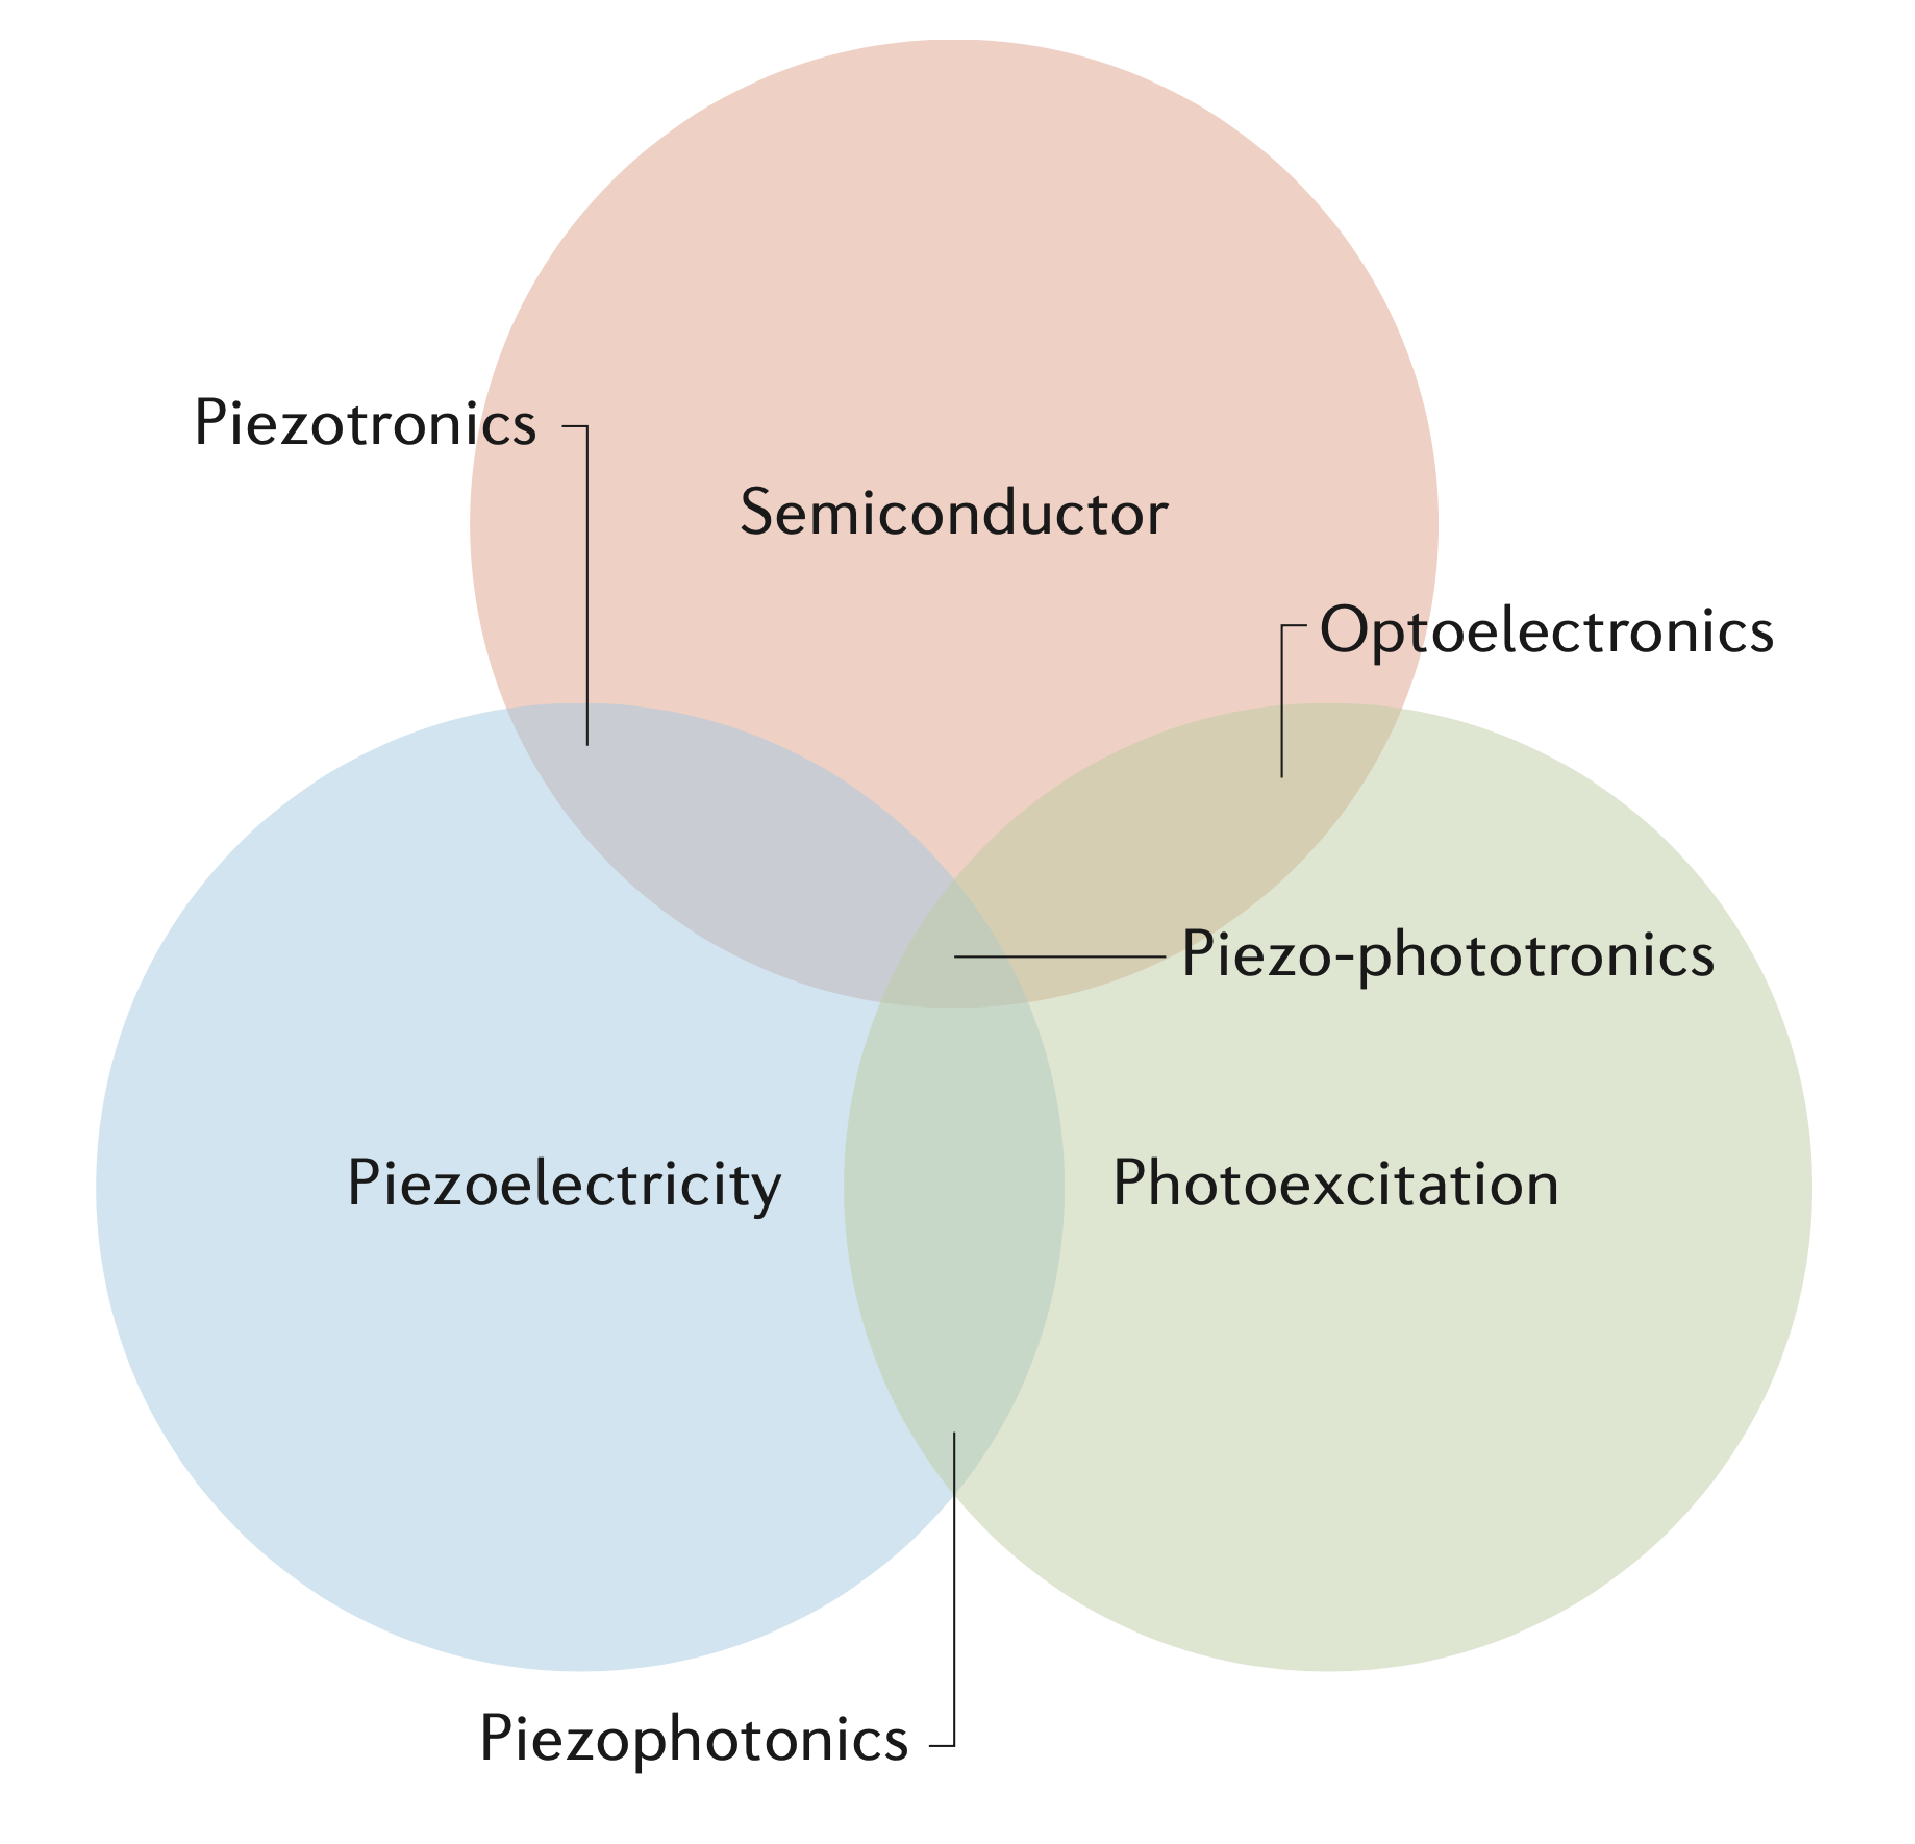
\includegraphics[width=0.7\textwidth]{ch1_1}
\caption[Coupling characteristics of piezotronics and piezo-phototronics]{Coupling characteristics of piezotronics and piezo-phototronics \protect\cite{wu2016piezotronics}}
\label{fig:1.1}
\end{figure}

The research of piezotronics \index{Piezotronics} effect mainly focus on the adjust/control the transport of carriers through piezoelectric potential \index{Piezoelectric!potential} generated by mechanical stress in semiconductor materials with piezoelectric \index{Piezoelectric!effect} properties. Therefore, according to this effect, the external stress can directly regulated the macroscopic electrical properties of piezoelectric semiconductor materials \cite{guo2017dynamic}. Among them, the Wurtzite \index{Wurtzite} crystal \index{Crystal} with hexagonal close-packed structure has good piezoelectric properties due to its non-centrosymmetric structure \cite{xin2007piezoelectricity}. Some of these materials have both piezoelectric and semiconductor properties, such as ZnO, GaN, InN and ZnS, etc., so they are widely used in piezotronics research. \autoref{fig:1.2} shows the piezoelectric potential in Wurtzite-structured ZnO nanowires. The $Zn^{2+}$ cation and $O^{2-}$ anion in ZnO are tetrahedral coordinated, and the centers of positive and negative ions overlap each other. If stress is applied at the vertices of the tetrahedron, the center of the cation and the center of the anion are displaced relative to each other and an electric dipole moment \index{Electric!dipole moment} is created (\autoref{fig:1.2}a). 

\begin{figure}[H] 
\centering    
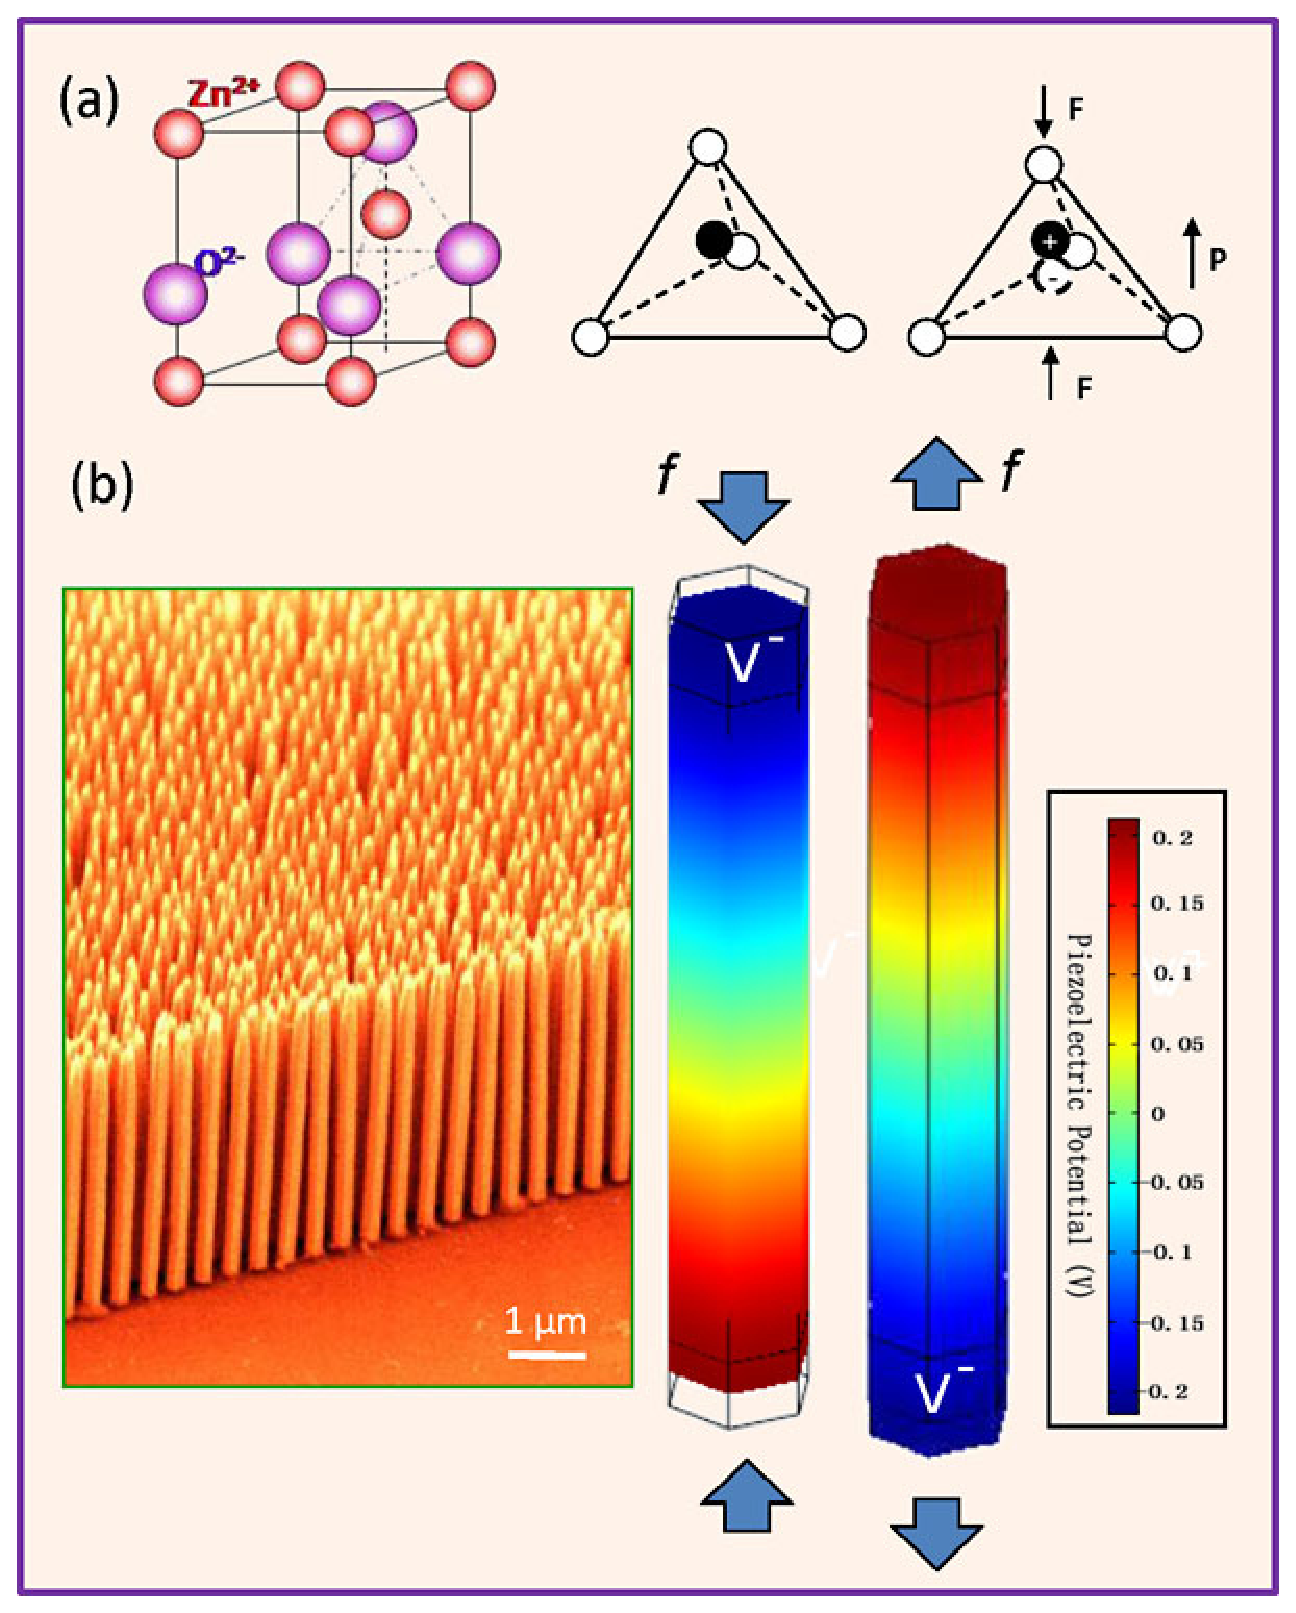
\includegraphics[width=0.7\textwidth]{ch1_2}
\caption[Piezopotential in wurtzite crystal ZnO]{Piezopotential in wurtzite crystal ZnO \protect\cite{wang2012piezotronics}}
\label{fig:1.2}
\end{figure}

The accumulation of electric dipole moments \index{Electric!dipole moment} generated by all units in the crystal \index{Crystal} leads to the generation of polarization charges \index{Polarization!charge} with the same density and opposite polarity at the interface \index{Interface} between the two ends of the crystal, resulting in a macroscopic potential along the strain \index{Strain} direction, that is, the \index{Piezoelectric!potential} piezoelectric potential (\autoref{fig:1.2}b). For a ZnO nanowire with a length of 1200 \unit{\nm} and a hexagonal length of 100 \unit{\nm}, a pulling force of 85 \unit{\nano\newton} produces a positive potential of approximately \SI{0.4}{\volt} between the two ends. When the applied force becomes compressive stress, the piezoelectric potential is reversed. The potential difference remains \SI{0.4}{\volt}, and the piezoelectric potential at both ends of the nanowire is the same in magnitude and opposite in polarity. The first systematic study of the \index{Piezoelectric!potential} piezoelectric potential in ZnO nanowires marked the beginning of the research of \index{Piezotronics} piezotronics \cite{wang2006piezoelectric}.

In piezoelectric semiconductor materials, the piezoelectric effect \index{Piezoelectric!effect} can significantly modulate the energy band \index{Energy band} structure of the material, thereby affecting the electrical properties of the material. Under the action of mechanical stress, piezoelectric polarization charges \index{Piezoelectric!polarization charge} with opposite polarities are generated at the interface \index{Interface} of the material. Piezoelectric polarization charges are distributed within a small depth from the surface \index{Surface} of the material, and they are non-mobile ionic charges located near the interface. In this case, due to the finite dielectric constant and limited doping concentration of the \index{Crystal} crystal, the free carriers can only partially shield the piezoelectric polarization \index{Piezoelectric!polarization charge} charge, but they cannot completely cancel the piezoelectric polarization charge. The piezoelectric potential \index{Piezoelectric!potential} formed by the piezoelectric polarization charges at the material interface can significantly change the contact properties of the semiconductor through the built-in \index{Electric!field} electric field, and thus the optical and electrical properties of the semiconductor contact can be directly modulated by external mechanical stress. Among them, Schottky \index{Contact!Schottky contact} contact, p-n junction, p-n heterojunction are the most common semiconductor contacts in piezoelectric semiconductor materials, so we briefly discuss the piezoelectric effects \index{Piezoelectric!effect} in these three semiconductor contacts (\autoref{fig:1.3}).

\begin{figure}[H] 
\centering    
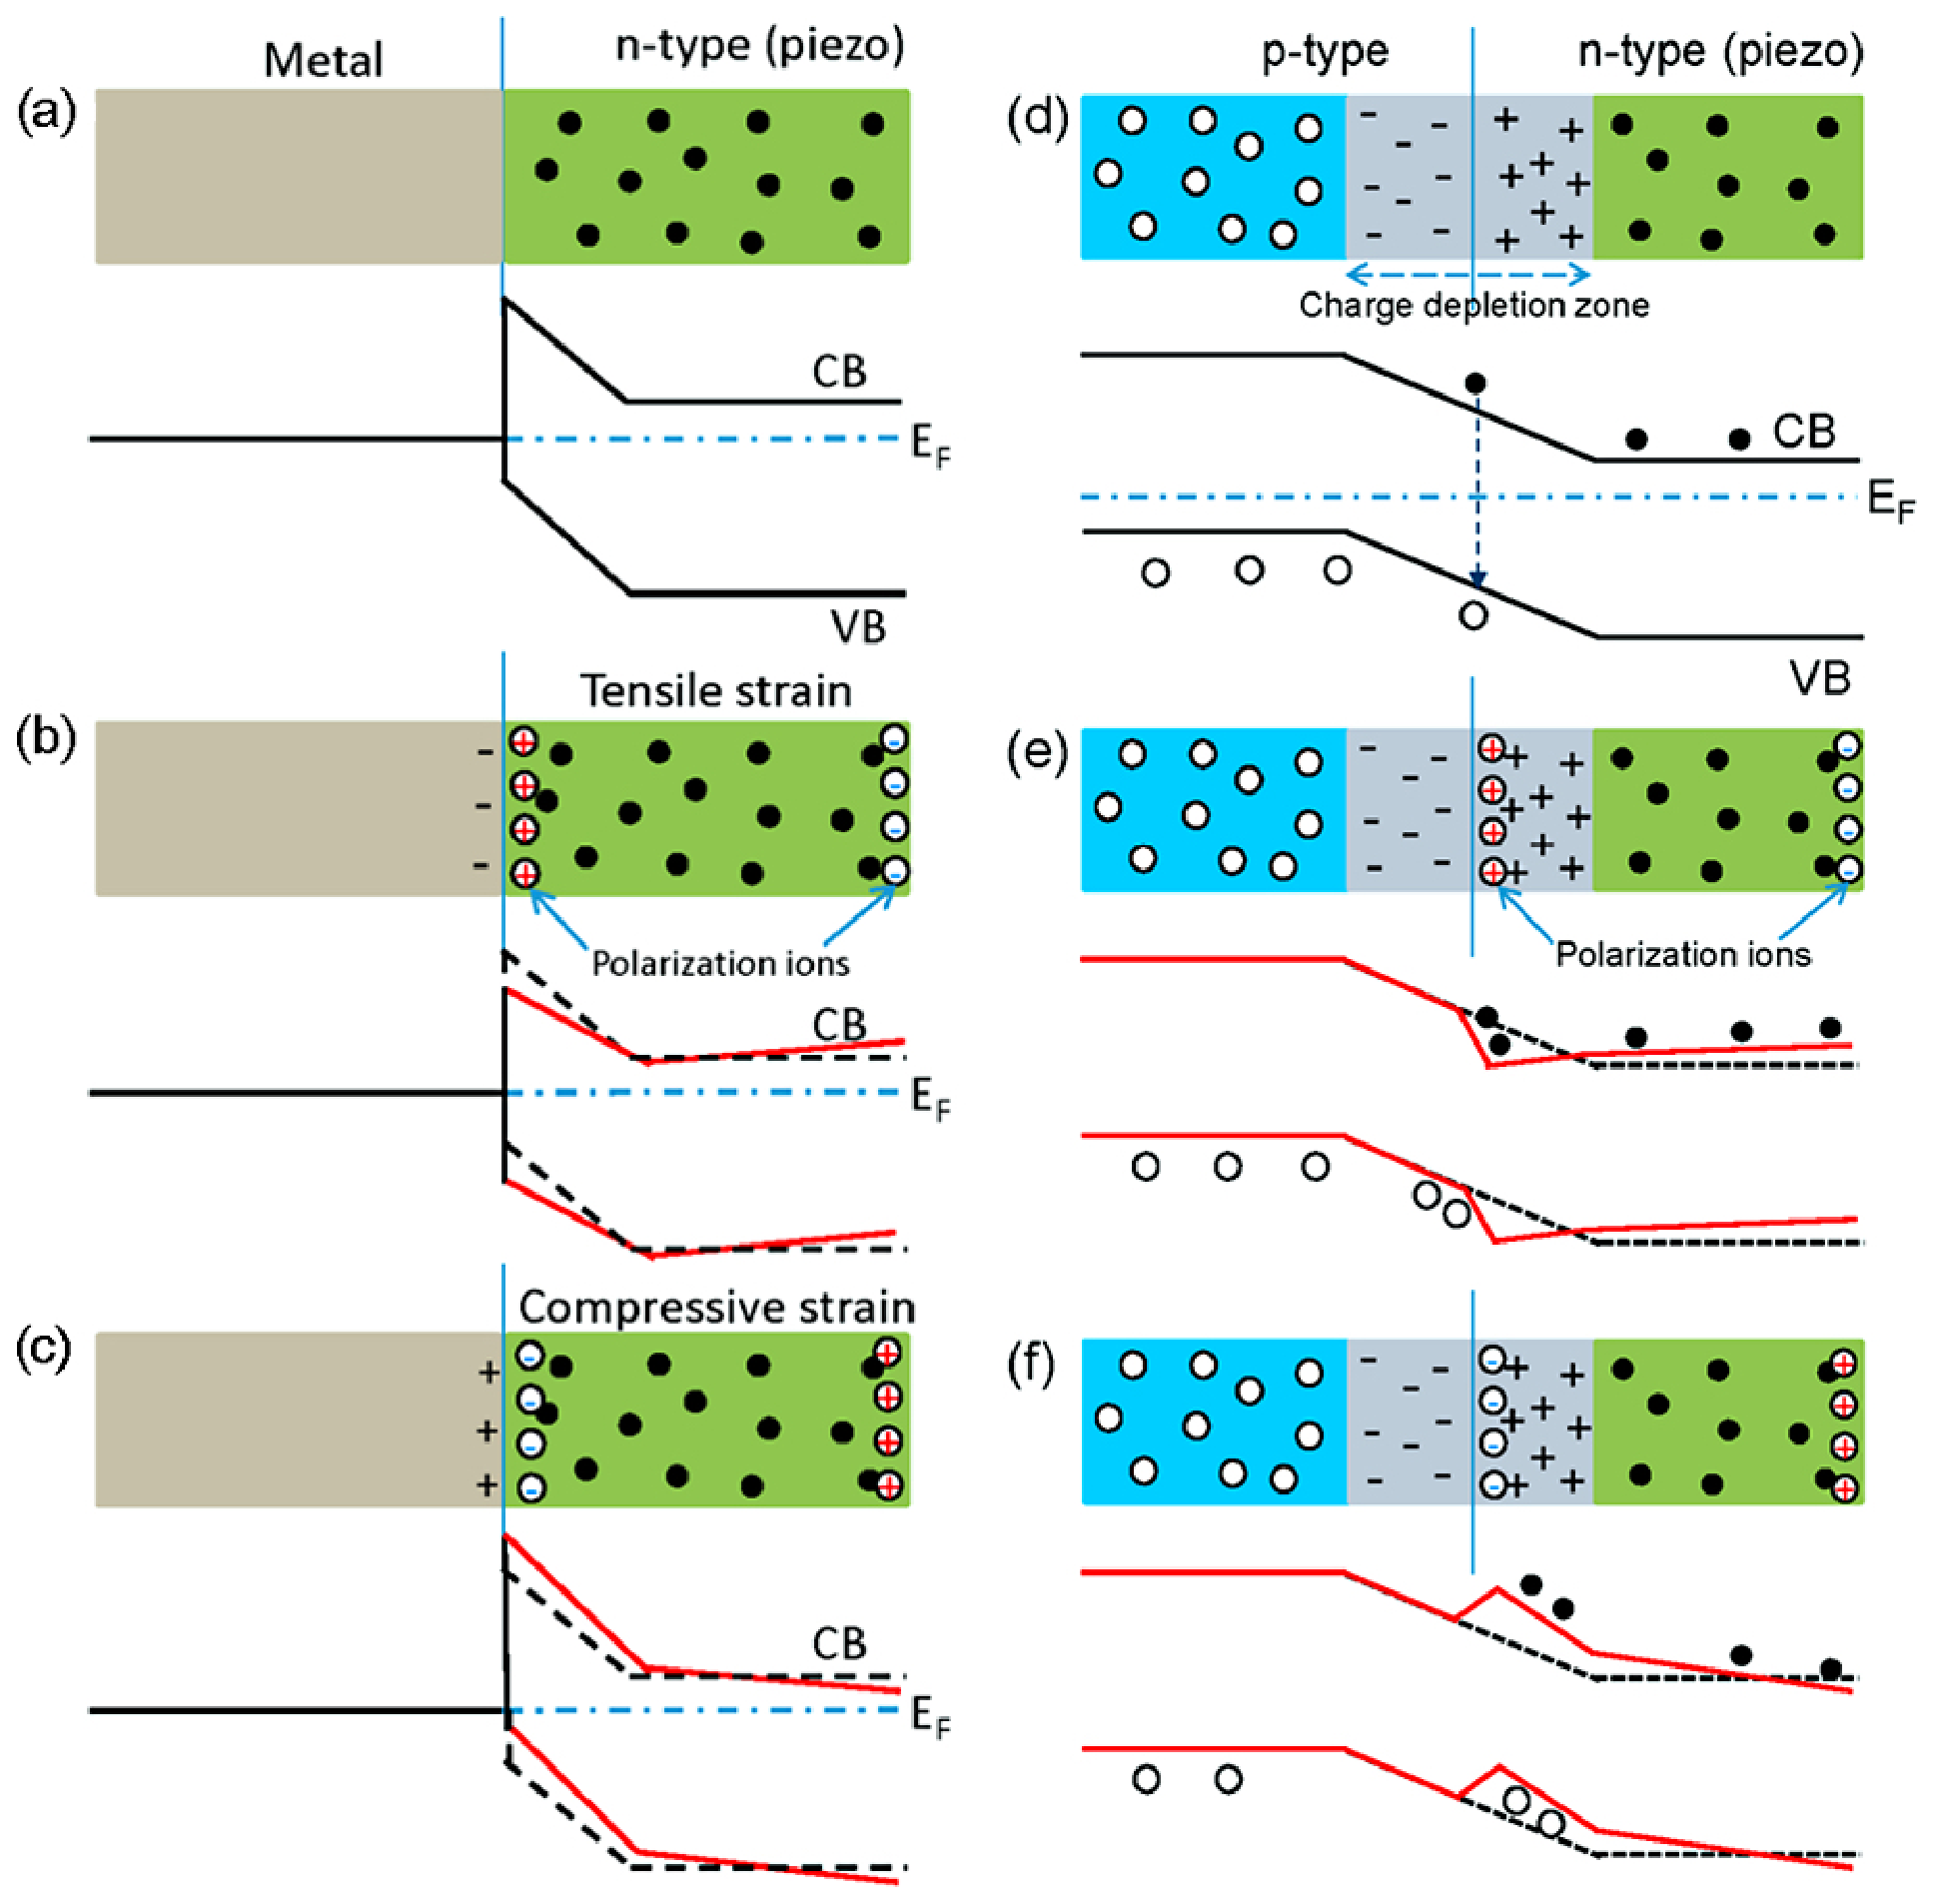
\includegraphics[width=0.9\textwidth]{ch1_3}
\caption[Energy band diagram of piezotronics effect in Schottky contact and p-n junction]{Energy band diagram of piezotronics effect in Schottky contact (a-c) and p-n junction (d-f) \protect\cite{wang2012piezotronics}}
\label{fig:1.3}
\end{figure}

In a Schottky contact \index{Contact!Schottky contact} formed by a metal material and a piezoelectric semiconductor material, strains \index{Strain} in different directions can generate piezoelectric polarization charges \index{Piezoelectric!polarization charge} with opposite polarizations at the interface \index{Interface} of the piezoelectric semiconductor material, and a negative piezoelectric polarization \index{Piezoelectric!polarization charge} charges at the metal-semiconductor material interface \index{Interface} can effectively reduce the local barrier height of Schottky \index{Contact!Schottky contact} contacts, while negative piezoelectric polarization charges \index{Piezoelectric!polarization charge} further increase the barrier height (\autoref{fig:1.3}a–c). The height of the Schottky \index{Contact!Schottky contact} barrier determines the carrier transport properties at the metal-semiconductor material interface, so we can directly modulate \index{Modulation} the electrical properties of the Schottky contact \index{Contact!Schottky contact} by external mechanical stress according to the piezotronics \index{Piezotronics} effect.

In a p-n junction composed of the same bandgap material, the interdiffusion and recombination of electrons and holes forms a depletion region in the junction region when the p-type and n-type semiconductors are in contact. The presence of such carrier-free regions can significantly enhance the piezotronics \index{Piezotronics} effect, since the piezoelectric polarization charges \index{Piezoelectric!polarization charge} here are not shielded by locally remaining free carriers. As shown in \autoref{fig:1.3}d-f, with the strain \index{Strain} applied to n-type piezoelectric semiconductor material, a net positive piezoelectric polarization charge \index{Piezoelectric!polarization charge} will be generated at the depletion region interface \index{Interface} if the doping concentration is relatively low. Piezoelectric potential \index{Piezoelectric!potential} tends to lower the local energy band \index{Energy band} slightly and introduce a slow slope into the energy band. When the applied strain \index{Strain} is in the opposite direction, the negative piezoelectric polarization charge \index{Piezoelectric!polarization charge} at the interface \index{Interface} of the depletion region raises the local energy \index{Energy band} band. The change of the energy band in the p-n junction can significantly affect the electron-hole recombination rate, which is very beneficial to improve the efficiency of LEDs. In addition, the degree of band tilt also affects the internal carrier mobility. Therefore, the piezotronics \index{Piezotronics} effect in the p-n junction can effectively tune its electrical and optical properties by external mechanical stress.

For p-n heterojunctions made of two materials with different band gaps, the piezoelectric polarization charge \index{Piezoelectric!polarization charge} also significantly affects the band distribution, as shown in \autoref{fig:1.4}. The black and red curves are used to represent the energy band \index{Energy band} diagrams of the p-n heterojunction before and after the external strain \index{Strain} in the eight cases, from which it can be seen that the transport characteristics of carriers at the interface \index{Interface} will be directly modulated \index{Modulation} by the \index{Piezoelectric!polarization charge} piezoelectric polarization charge. Take the case shown in \autoref{fig:1.4}e as an example: the height of the barrier formed at the interface \index{Interface} is reduced due to the reduction of the energy band \index{Energy band} caused by the \index{Piezoelectric!polarization charge} piezoelectric polarization charge, so that electrons can be transported across the interface \index{Interface} more efficiently. In contrast to \autoref{fig:1.4}f, the height and width of the potential barrier at the interface increase due to \index{Piezoelectric!polarization charge} piezoelectric polarization charges, hindering the transport of electrons

\begin{figure}[H] 
\centering    
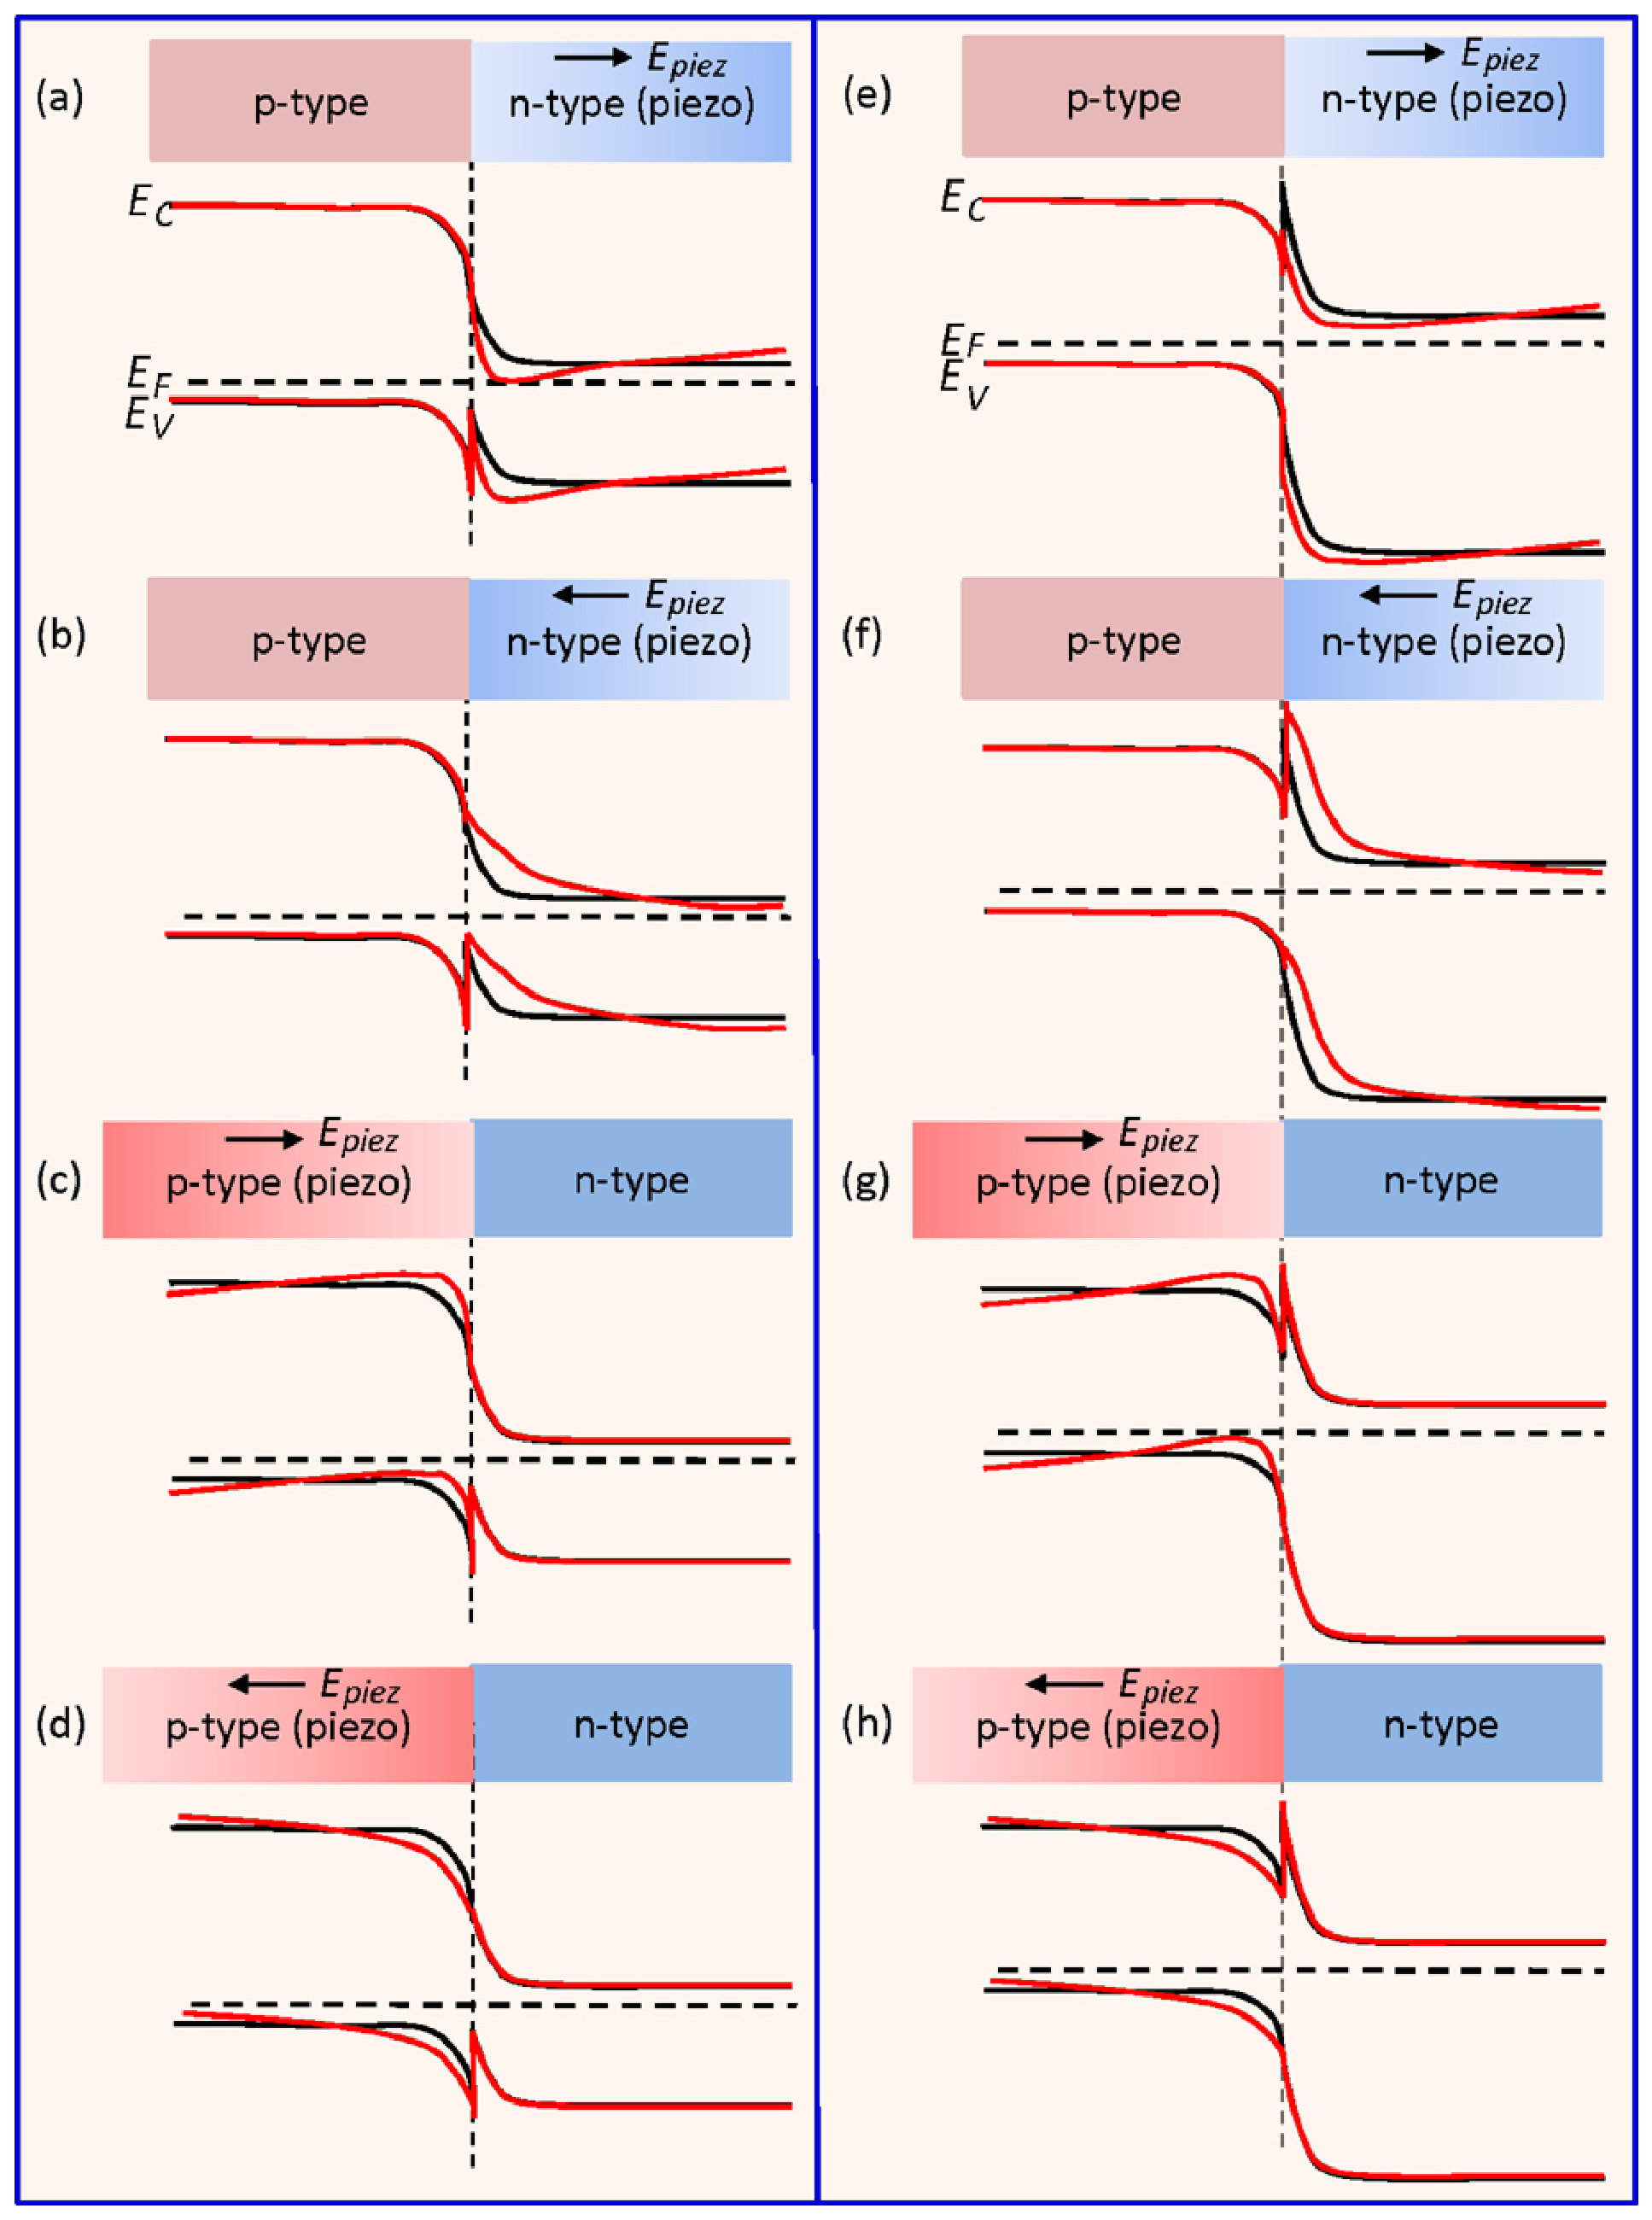
\includegraphics[width=0.9\textwidth]{ch1_4}
\caption[Energy band diagram of piezotronic effect in p-n heterojunction]{Energy band diagram of piezotronic \index{Piezotronics} effect in p-n heterojunction \protect\cite{wang2012piezotronics}}
\label{fig:1.4}
\end{figure}

\noindent across the \index{Interface} interface. For the case shown in \autoref{fig:1.4}b, the reorganization of the energy band \index{Energy band} caused by the piezoelectric polarization charge \index{Piezoelectric!polarization charge} can significantly increase the local trapping of holes and improve the luminous efficiency of the LED. But for the case of \autoref{fig:1.4}a, the reformation of the energy bands \index{Energy band} negatively affects the efficiency of the LED. Therefore, based on the piezotronics \index{Piezotronics} effect, the external strain \index{Strain} in the heterojunction can effectively tune the optoelectronic properties of the material.

Piezotronics \index{Piezotronics} transistors can be designed and fabricated based on the modulation \index{Modulation} properties of piezoelectric polarization charges \index{Piezoelectric!polarization charge} in piezoelectric semiconductor materials. For a conventional \index{Channel} n-channel metal-oxide-semiconductor field-effect transistor MOSFET (Fig. 1.5a), the drain and source are two n-type doped regions, and a thin metal insulating oxide layer is deposited on the p-type region to form the Schottky contact \index{Contact!Schottky contact} as the gate. The \index{Voltage!gate voltage} gate voltage $V_{G}$ controls the channel \index{Channel} width of the transport carriers, so the current flowing from the drain to the source under the source-drain bias voltage $V_{DS}$ is controlled by the gate voltage $V_{G}$. Similarly, for a single-channel FET (\autoref{fig:1.5}b) fabricated using semiconducting nanowire materials, the drain and source are two metal electrodes, and the current is regulated by applying a gate voltage \index{Voltage!gate voltage} on top of the nanowire. A piezotronics \index{Piezotronics} transistor is a metal-nanowire-metal structure, such as Au-ZnO-Au or Ag-ZnO-Ag, as shown in \autoref{fig:1.5}c,d. The basic principle of piezotronics \index{Piezotronics} transistor is to generate a piezoelectric potential \index{Piezoelectric!potential} at the interface \index{Interface} of the semiconductor by applying external \index{Strain} strain, thereby regulating the local energy band \index{Energy band} at the contact, and finally realizing the control of the carrier transport characteristics at the metal-semiconductor interface. Therefore, unlike conventional MOSFETs, in piezotronics \index{Piezotronics} transistor based on the piezoelectric \index{Piezoelectric!effect} effect, the externally applied gate voltage \index{Voltage!gate voltage} that controls the channel \index{Channel} width is replaced by a \index{Strain} strain-generated piezoelectric \index{Piezoelectric!potential} potential, thus eliminating the "gate". Piezotronics \index{Piezotronics} transistor are a new type of transistors that replace voltage control with external \index{Strain} strain/stress control, and have broad application prospects.

\begin{figure}[H] 
\centering    
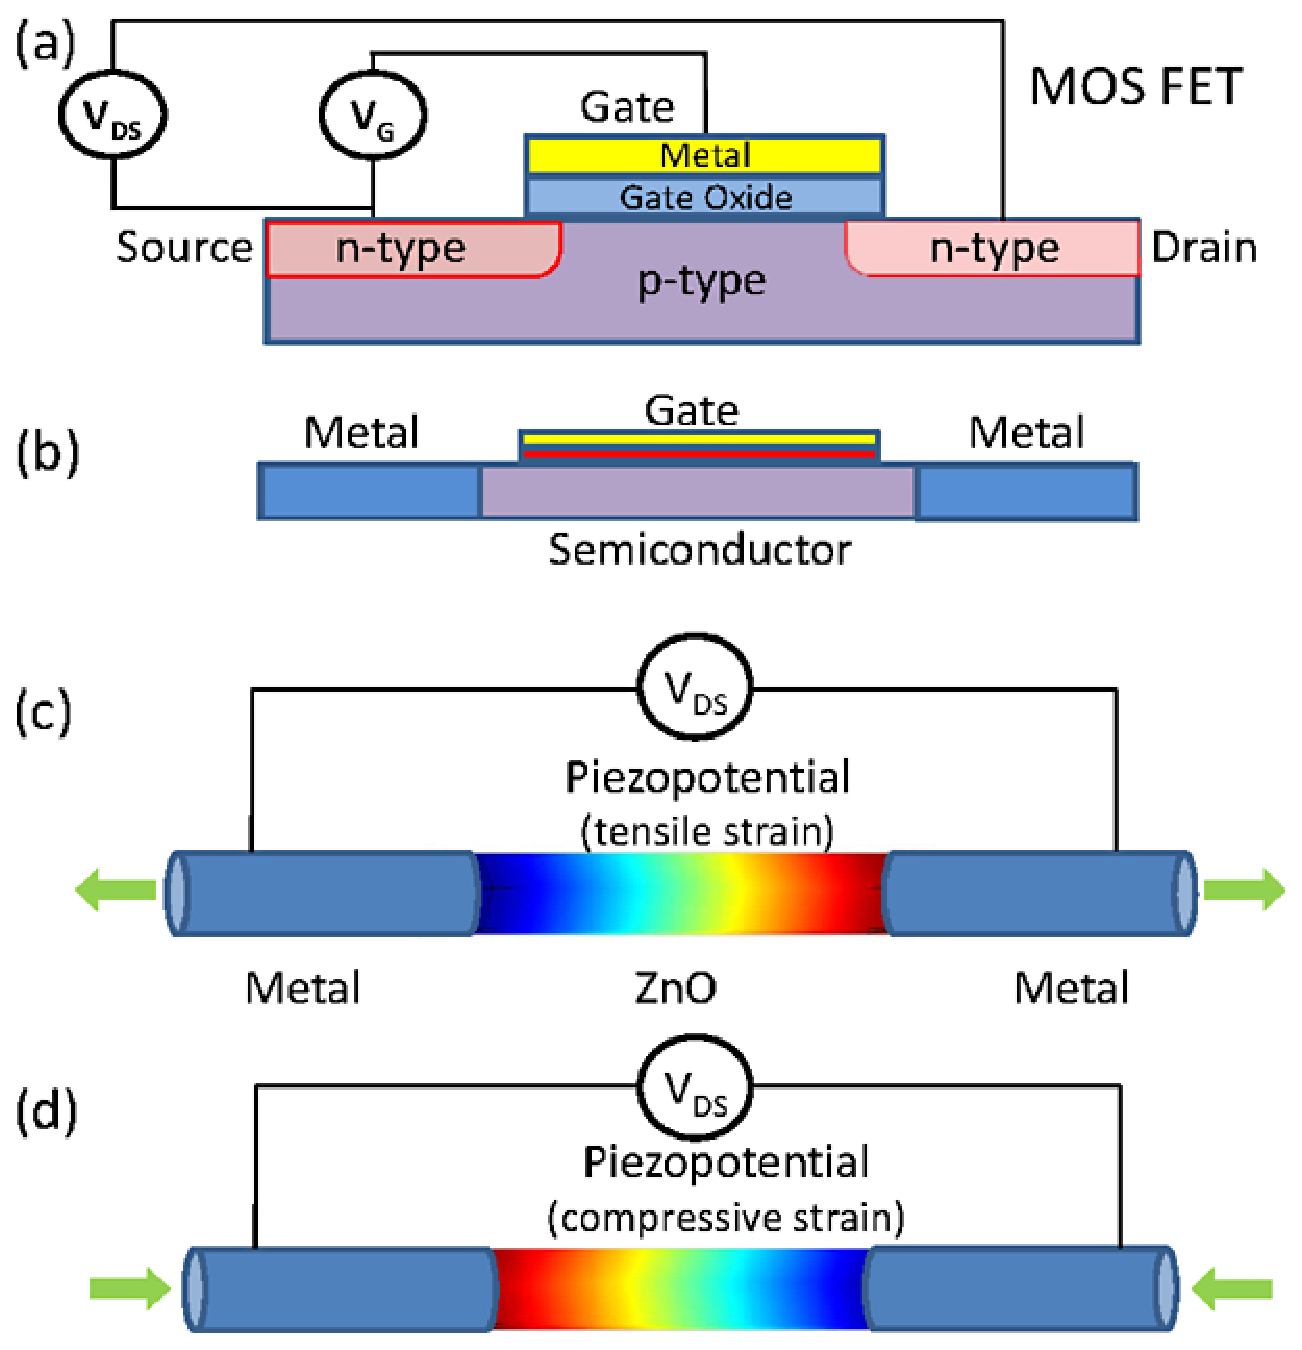
\includegraphics[width=0.7\textwidth]{ch1_5}
\caption[Working principle of piezotronics transistor]{Working principle of piezotronics transistor. (a) The n-channel MOSFET; (b) The semiconductor nanowire FET; The piezotronics transistor with tensile strain (c) and compressive strain (d) \protect\cite{wang2012piezotronics}}
\label{fig:1.5}
\end{figure}

\subsection{Application prospect of piezotronics effect}

The study of piezotronics \index{Piezotronics} effects, ie the study of the coupling properties of piezoelectric and semiconductor properties in piezoelectric semiconductor materials, has given rise to a whole new range of applications. By using piezoelectric potential \index{Piezoelectric!potential} as the gate voltage \index{Voltage!gate voltage} to modulate \index{Modulation} the transport properties of electrons, researchers have fabricated transistors, sensors and smart devices driven and controlled by external stress, including piezoelectric potential \index{Piezoelectric!potential} gate field effect transistors \cite{wang2006piezoelectric-nl}, piezoelectric potential \index{Piezoelectric!potential} gated diodes \cite{he2007piezoelectric}, strain sensor \cite{zhou2008flexible}, force/flow sensor \cite{fei2009piezoelectric}, hybrid field effect transistor \cite{liu2010piezopotential}, piezoelectric logic gate \cite{wu2010strain}, electromechanical memory \cite{wu2011piezotronic}, etc. Piezotronics \index{Piezotronics} devices have been regarded as a new class of semiconductor devices with important applications in sensors, human-machine interfaces, MEMS, nanorobots, and flexible electronics (\autoref{fig:1.6}).

\begin{figure}[H] 
\centering    
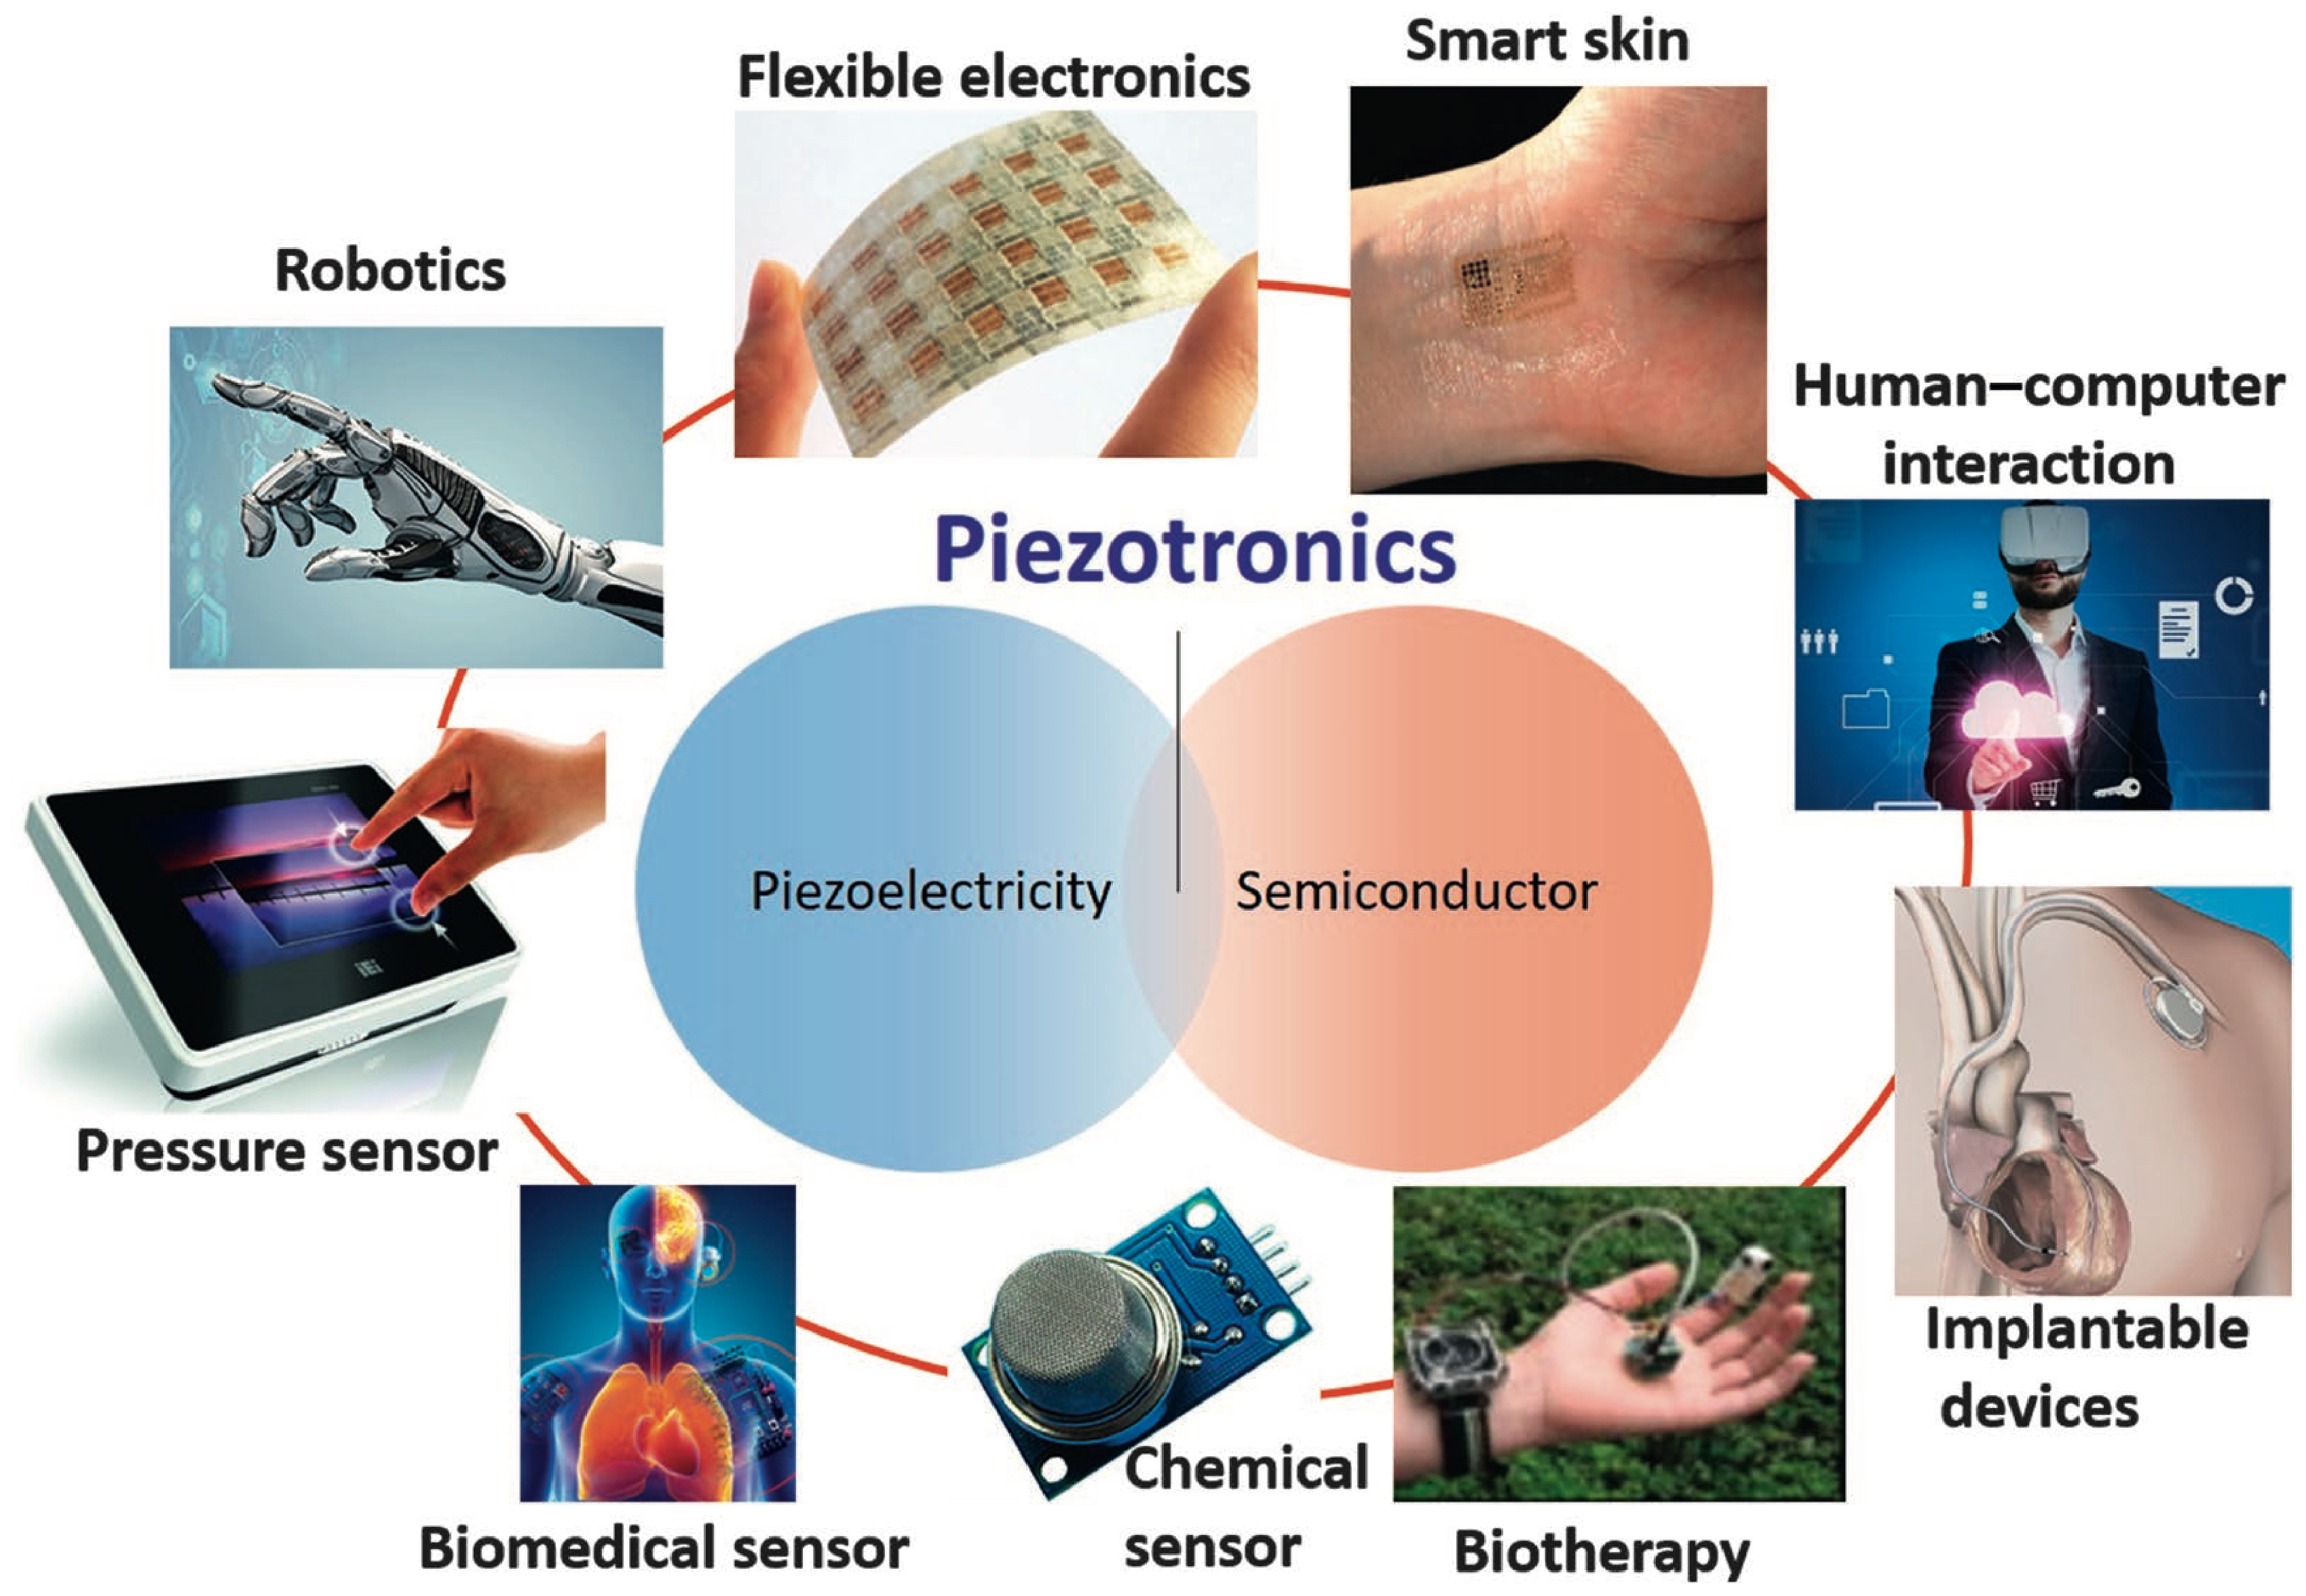
\includegraphics[width=0.9\textwidth]{ch1_6}
\caption[The application prospects and future prospects of piezotronics]{The application prospects and future prospects of piezotronics \protect\cite{hu2018piezotronic}}
\label{fig:1.6}
\end{figure}

%********************************** %Second Section  *************************************
\section{Piezotronics effects in III-V nitrides} 
\subsection{Crystal structure and polarization properties of III-V nitrides}

Group III-V nitride \index{Nitride} materials are compound semiconductor materials formed by group III elements Al, Ga, In and group V elements N, such as GaN, InN, AlN and multi-element alloy materials ($In_{x}Ga_{1-x}N$, $Al_{x}Ga_{1-x}N$, etc.). There are usually two different lattice structures of hexagonal \index{Wurtzite} wurtzite (Wurtzite) and cubic sphalerite (Zinc-blende). Among them, the nitride crystal \index{Crystal} of wurtzite structure is more stable and is widely used in semiconductor materials. This research focuses on GaN, AlN and $Al_{x}Ga_{1-x}N$  semiconductor materials. 

\begin{figure}[H] 
\centering    
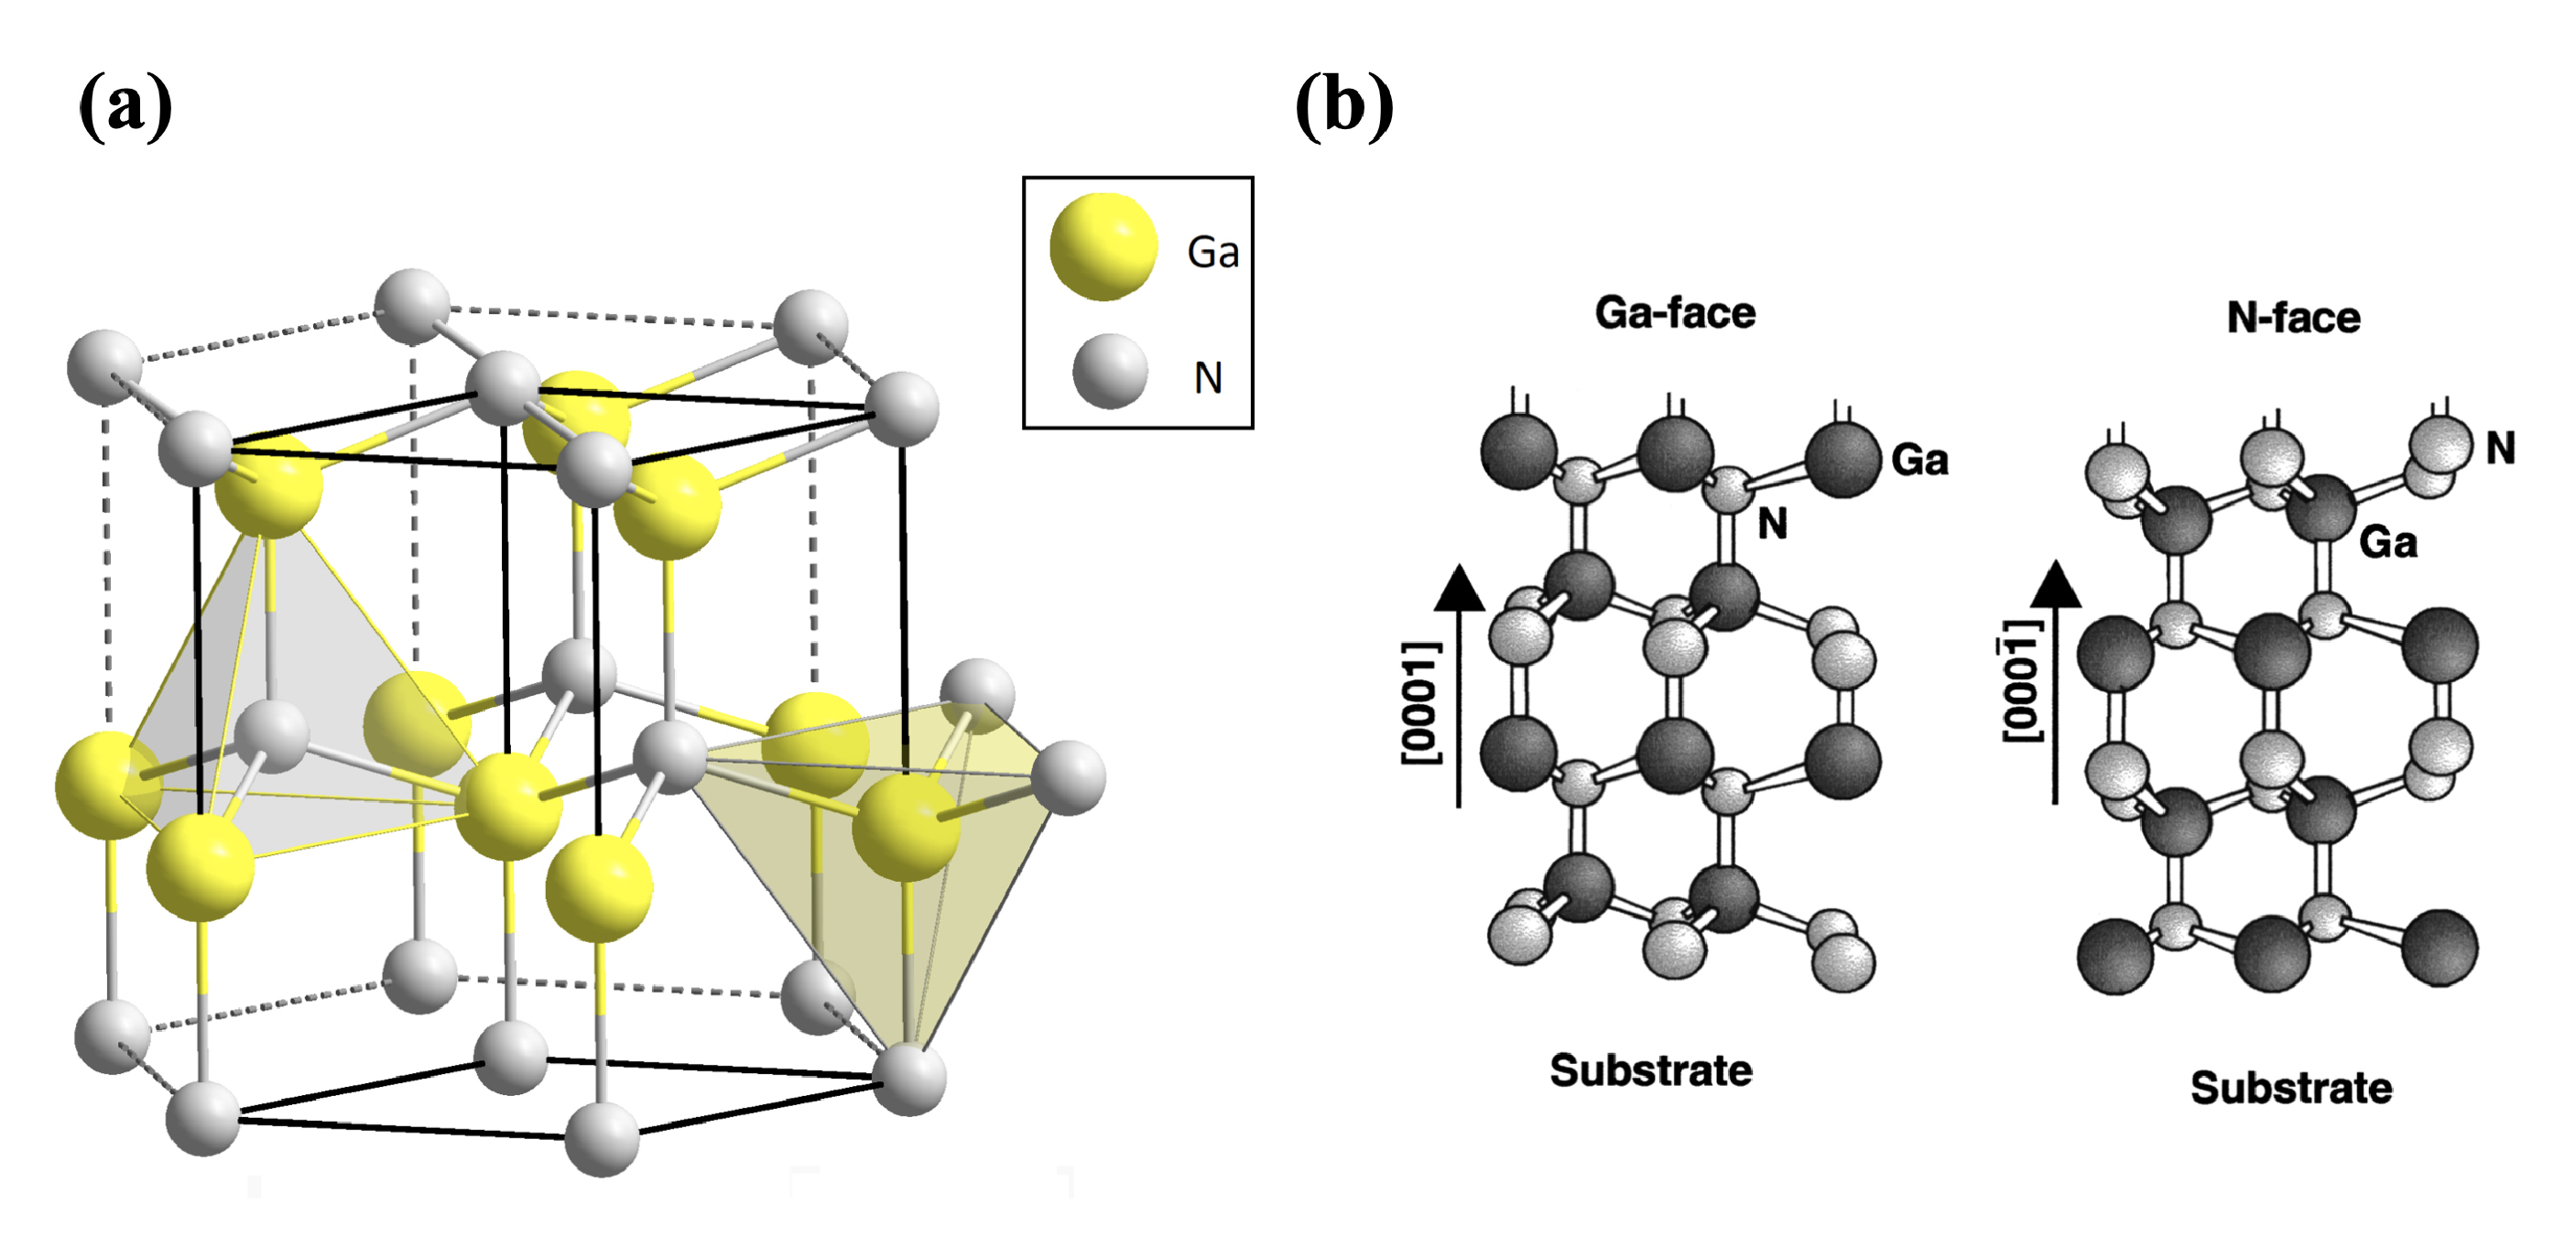
\includegraphics[width=0.9\textwidth]{ch1_7}
\caption[The wurtzite crystal structure of GaN material and the polarization characteristics of the Ga and N plane]{The wurtzite crystal structure of GaN material and the polarization characteristics of the Ga and N plane}
\label{fig:1.7}
\end{figure}

\autoref{fig:1.7}a shows the wurtzite \index{Wurtzite} structure of GaN \index{Crystal} crystal. Since the wurtzite structure of GaN crystal \index{Crystal} belongs to the non-centrosymmetric crystal, the crystal pole axis is the c-axis, and the atomic layers are are aligned along the c-axis from two different directions $[0001]$ and $[000\overline{1}]$, thus forming two distinct polar faces. It can be seen from \autoref{fig:1.7}b that when accumulating from the bottom to the top along the $[0001]$ direction, the top is the Ga atomic plane, which causes the Ga surface \index{Surface} polarity to be generated on the surface of the material; when accumulating from the bottom to the top along the $[000\overline{1}]$ direction, the top is the N atomic plane so that the N-plane polarity is generated on the surface of the material \cite{hellman1998polarity}. Since the electronegativity \index{Electronegativity} of negative ions formed by N atoms is stronger than that of positive ions formed by Ga atoms, a built-in electric field \index{Electric!field} will be generated. The direction of the electric field is from Ga atoms to N atoms along the c-axis. This phenomenon is called Spontaneous \index{Spontaneous polarization} Polarization \index{Polarization!effect} effect of GaN crystal \cite{sacconi2001spontaneous,yu1999spontaneous}. Generally, the spontaneous polarization direction of Ga-plane polarity GaN crystals is that the surface points to the inside, and the upper surface of the material gathers negative polarized charges and is negatively charged. The spontaneous polarization \index{Spontaneous polarization} direction of N-plane polarity GaN crystals \index{Crystal} is that the interior points to the surface. The upper surface \index{Surface} is positively charged by accumulating positive polarized charges. This phenomenon is more obvious in the Al-N atomic pair, so the same spontaneous polarization effect also exists in the AlGaN compound semiconductor material. In addition, if the GaN lattice is subjected to compressive or tensile deformation \index{Deformation} due to mechanical stress, it will cause lattice strain \index{Lattice!strain} within a certain range. At this time, the centers of $Ga^{+}$ ions and $N^{-}$ ions will be separated to form an \index{Electric!dipole moment} electric dipole moment, and the surface \index{Surface} of the material will also appear polarization \index{Polarization!charge} charge. This effect is called Piezoelectric Polarization \index{Piezoelectric!polarization} effect of GaN crystal \cite{sacconi2001spontaneous,yu1999spontaneous}. Therefore, the \index{Crystal} GaN crystal is also known as piezoelectric semiconductor material.

GaN and its corresponding Al and In composition compound semiconductor materials have unique material and electrical properties due to \index{Piezoelectric!effect} piezoelectric effect, such as changing Al composition in AlGaN/GaN heterojunction to adjust the degree of lattice mismatch \index{Lattice!mismatch} between AlGaN and GaN so as to generate corresponding \index{Piezoelectric!polarization charge} piezoelectric polarization charges, thereby modulating \index{Modulation} the energy band \index{Energy band} at the heterojunction and forming a two-dimensional electron gas (2DEG) \index{Two-dimensional electron gas (2DEG)} with high density and high \index{Electron mobility} electron mobility. The method of modulating the energy band \index{Energy band} and electrical properties by the polarization effect \index{Polarization!effect} is called Polarization Engineering \index{Polarization!engineering} \cite{hao2016nitride,jena2010polarization}. \autoref{fig:1.8} shows the strain-induced \index{Strain} piezoelectric polarization charge \index{Piezoelectric!polarization charge} density and the direction of spontaneous \index{Spontaneous polarization} and piezoelectric polarization \index{Piezoelectric!polarization} in an AlGaN/GaN heterojunction with Ga- and N-plane polarities. Therefore, III-V nitride \index{Nitride} compound semiconductor materials couple piezoelectric properties and semiconductor properties, and exhibits significant piezotronics \index{Piezotronics} effects \cite{pan2019piezotronics,sha2019iii,wang2018piezotronics}. Piezoelectric polarization charges generated at the interface by external strain can modulate the energy band of the heterojunction and the two-dimensional electron gas (2DEG) concentration \index{Two-dimensional electron gas (2DEG)} in the potential \index{Potential!well} well \cite{lev2018k}. In recent years, several studies have shown that the \index{Strain} strain-induced piezoelectric polarization charge at the AlGaN/GaN heterojunction interface \index{Interface} has been used to tune the piezoelectric nanowires \cite{wang2016piezotronic}, LEDs \cite{huang2016piezo,liu2020piezo,guo2021enhanced} and HEMTs \cite{liu2017electrical,jiang2017piezotronic,zhu2019piezotronic} based on the piezotronics effect.

\begin{figure}[H] 
\centering    
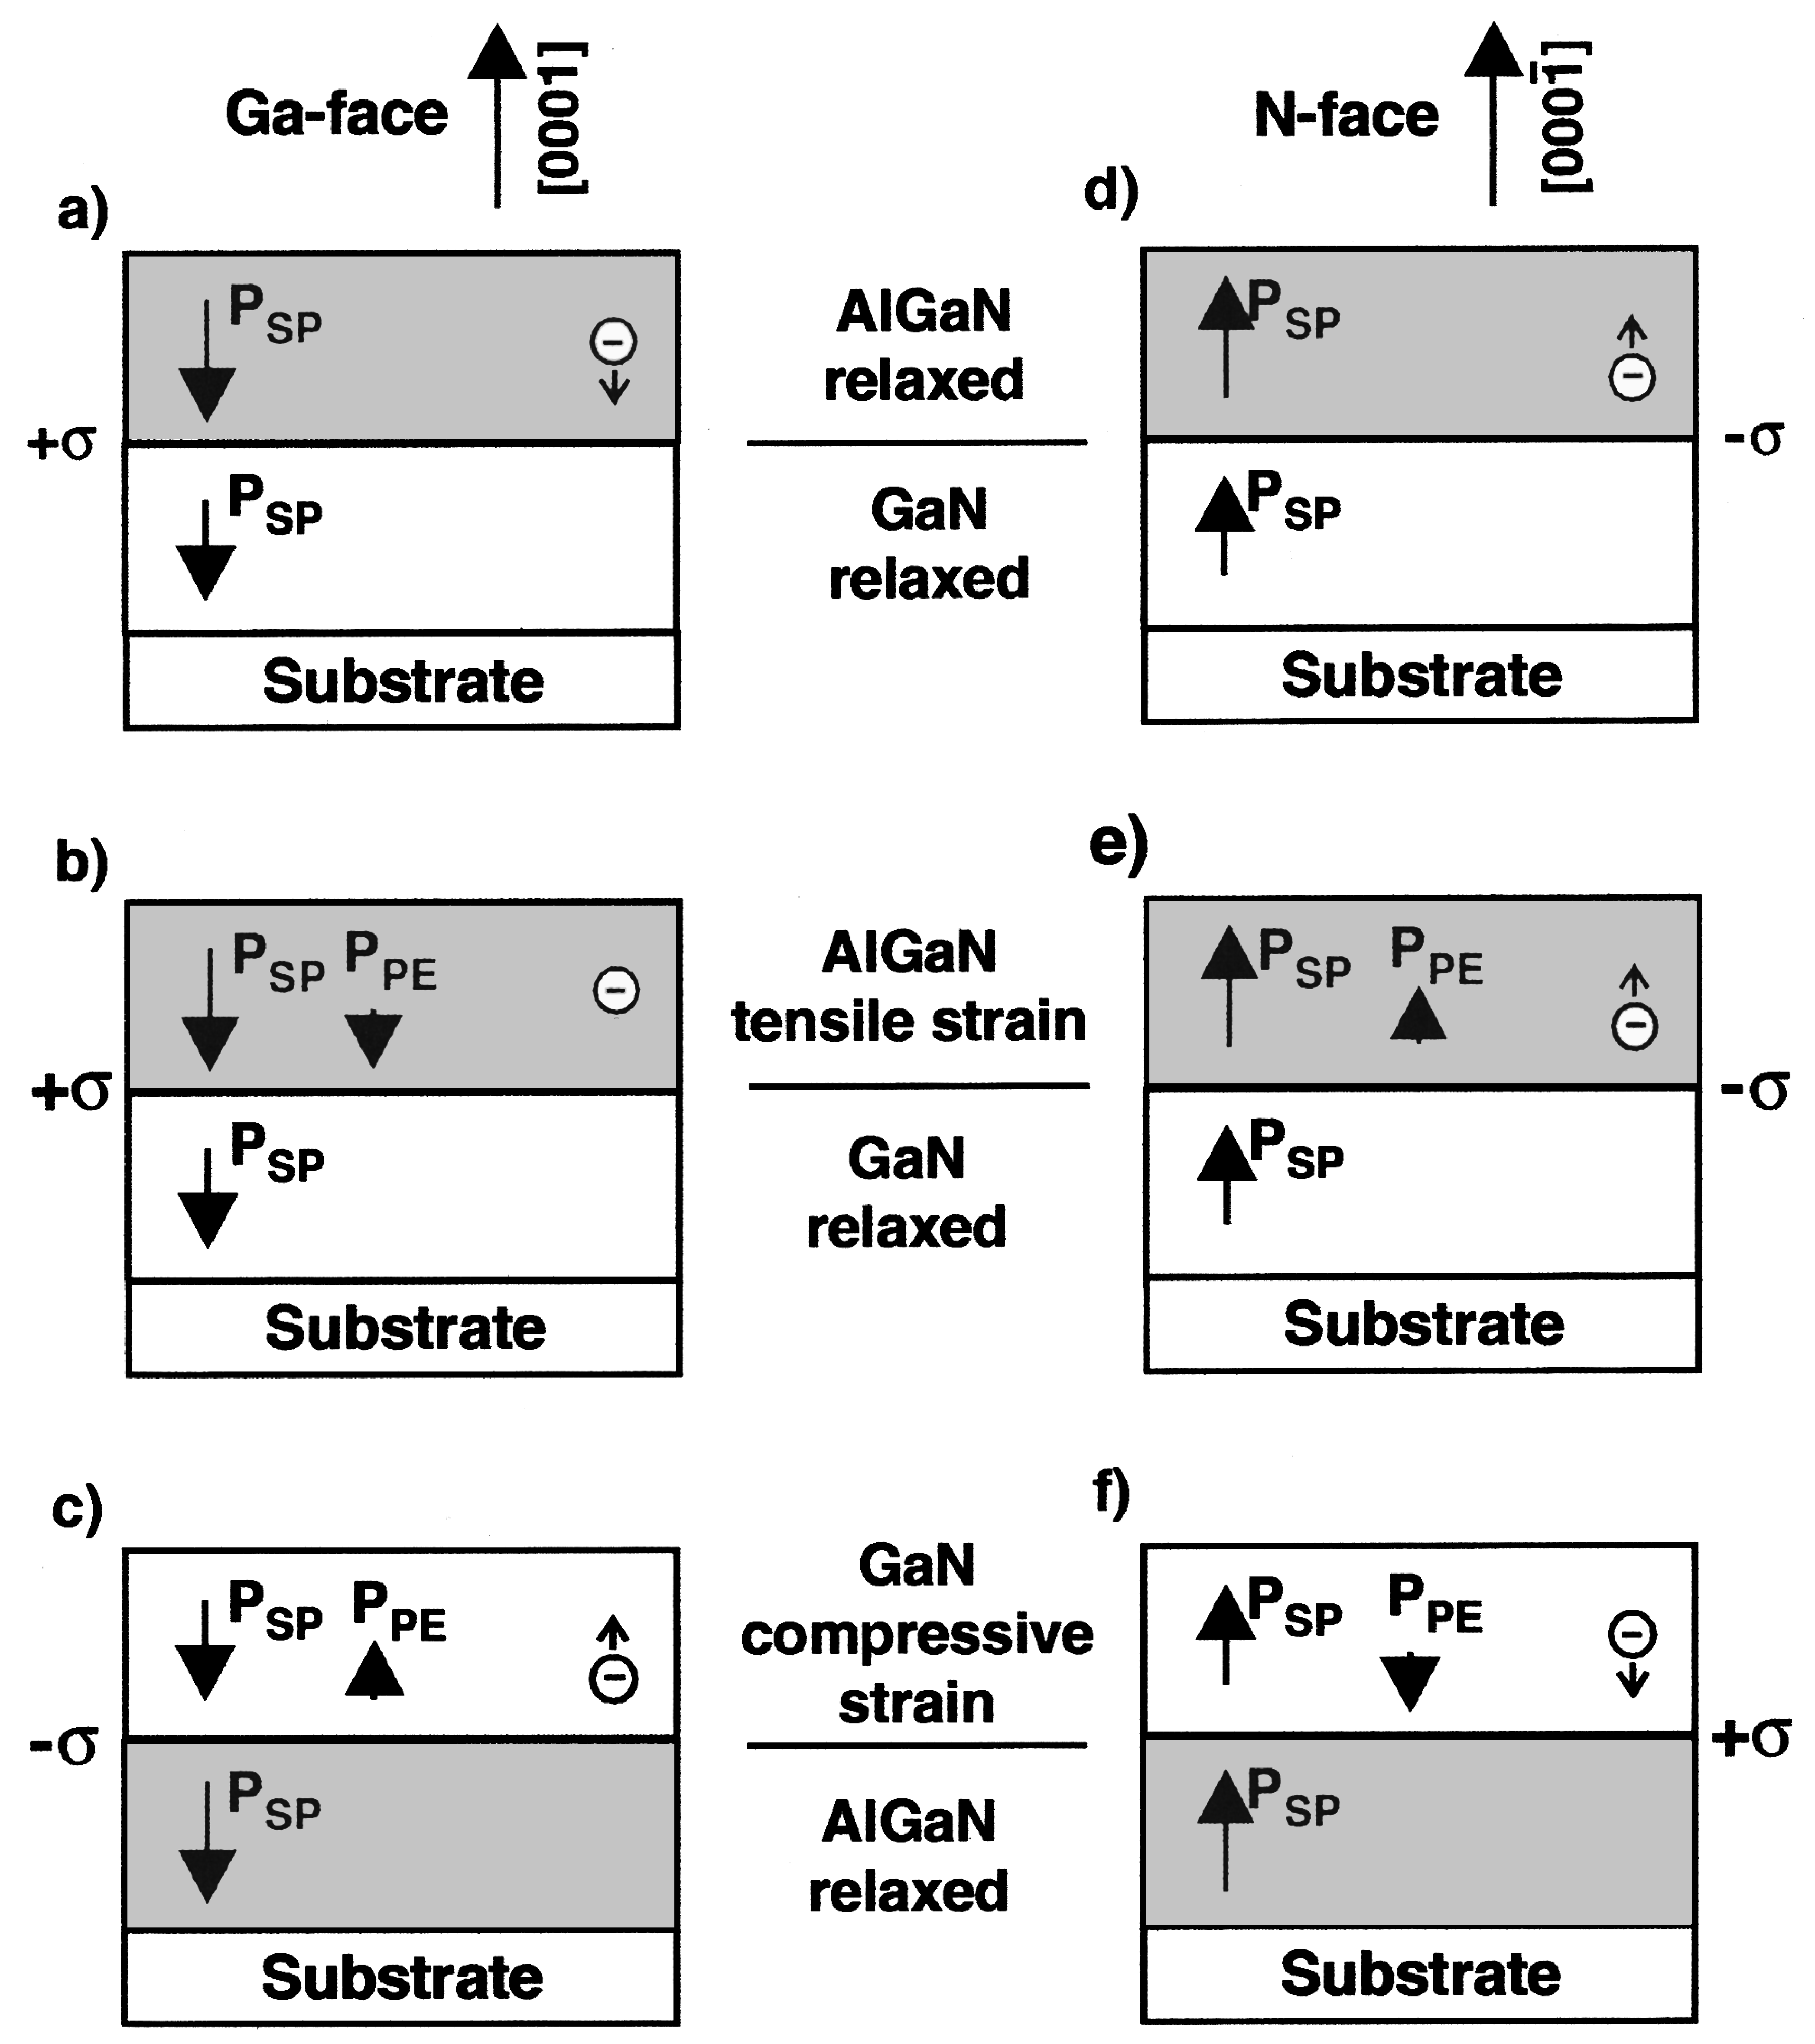
\includegraphics[width=0.9\textwidth]{ch1_8}
\caption[Polarization charge in AlGaN/GaN heterojunction with Ga-plane and N-plane polarity]{Polarization charge in AlGaN/GaN heterojunction with Ga-plane and N-plane polarity \protect\cite{ambacher1999two}}
\label{fig:1.8}
\end{figure}

\subsection{Application of piezotronics effect in III-V nitride}

Piezotronics \index{Piezotronics} effects have been widely used in the study of III-V \index{Nitride} nitrides. Wang et al. were the first to study the piezotronics effect in AlGaN/AlN/GaN heterostructured \index{AlGaN/AlN/GaN heterojunction} microwires and applied it as a novel approach to tune the physical properties of \index{Heterojunction electron gas (HEG)} heterojunction electron gas (HEG) \cite{wang2016piezotronic}. Unlike conventional approaches to tune HEG properties by changing the alloy composition or controlling the thickness of the heterojunction film, this work exploits \index{Strain} strain-induced piezoelectric polarization charges \index{Piezoelectric!polarization charge} to modify the local energy band \index{Energy band} distribution at the heterojunction, as shown in \autoref{fig:1.9}. By introducing piezotronics \index{Piezotronics} effects into AlGaN/AlN/GaN heterostructure microwires, the electrical conductivity \index{Electrical!conductivity} of \index{Heterojunction electron gas (HEG)} HEG increases by 165$\%$ at -1.78$\%$ compressive strain and decreases by 48$\%$ at 1.78$\%$ tensile strain at room temperature. This modulation \index{Modulation} is further enhanced by 890$\%$ and 940$\%$ under compressive and tensile strains, respectively, due to the enhanced piezoelectric effect \index{Piezoelectric!effect} at lower ambient temperature of 77 \unit{\kelvin}. This study provides insight into the piezotronics \index{Piezotronics} effects of low-dimensional electron gas in heterostructured nanomaterials with potential applications in HEMT \index{HEMT} and \index{MEMS} MEMS/NEMS.

\begin{figure}[H] 
\centering    
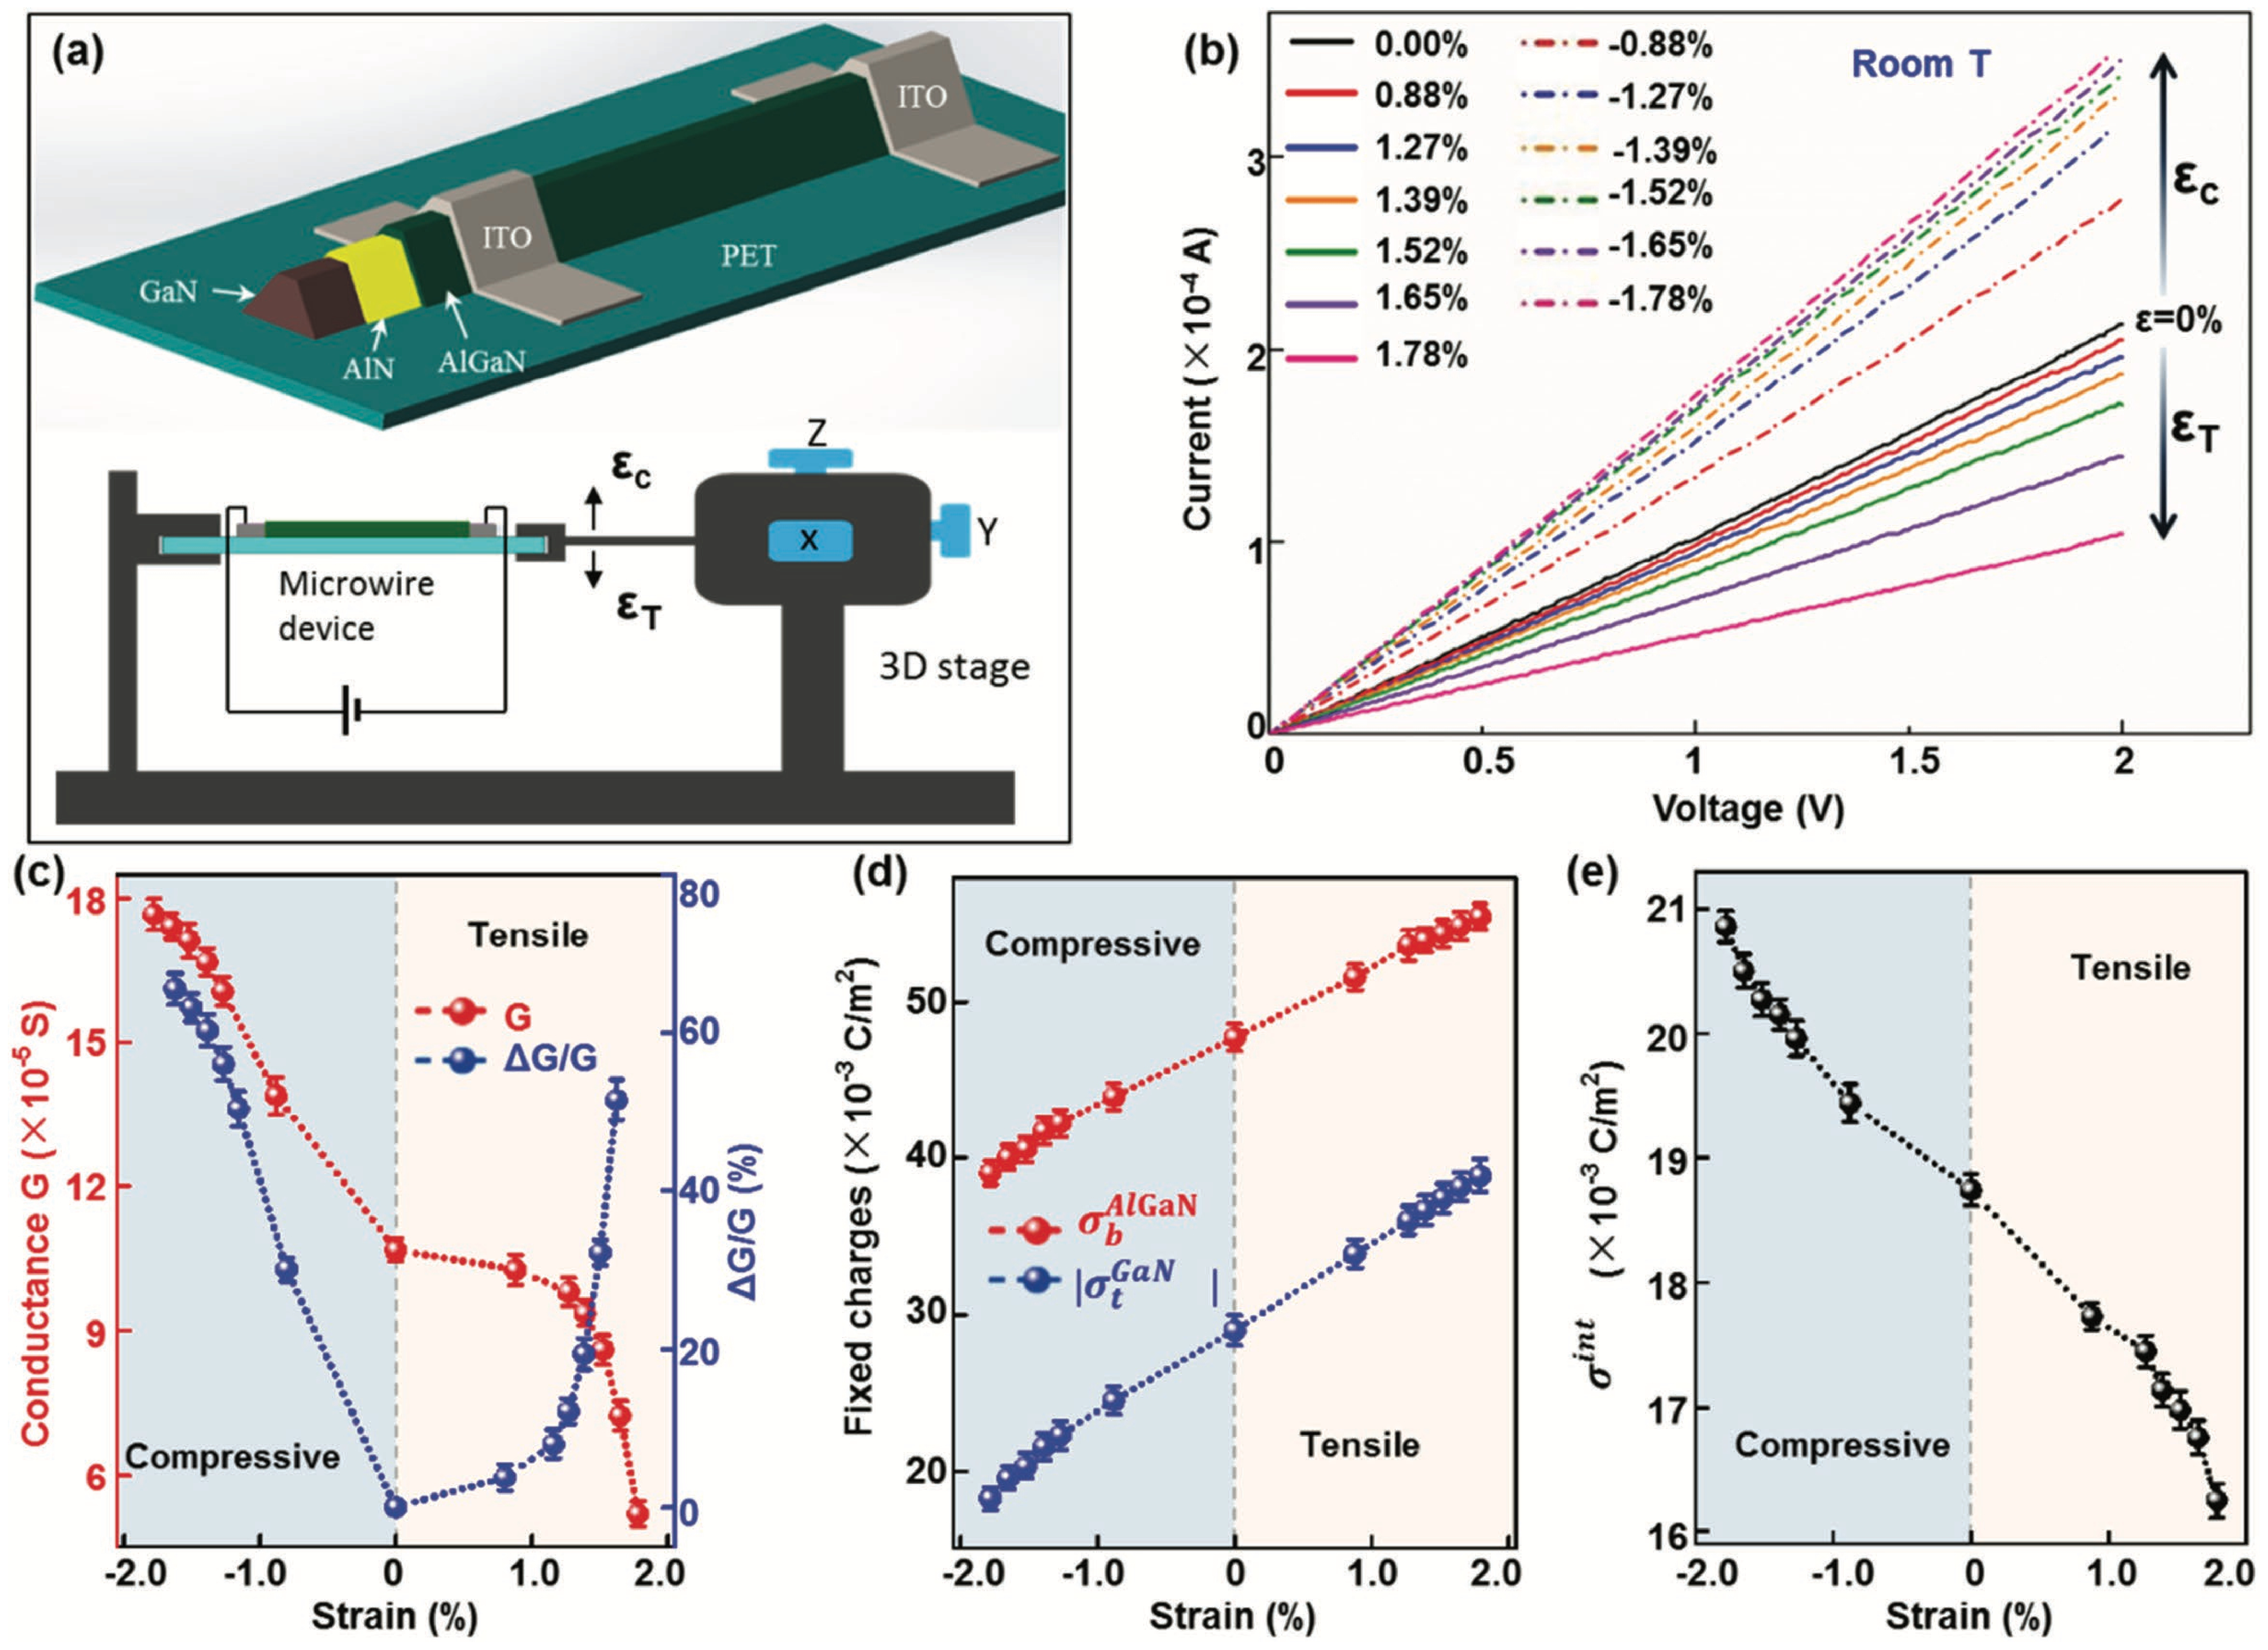
\includegraphics[width=0.9\textwidth]{ch1_9}
\caption[Piezotronic effect in AlGaN/AlN/GaN heterostructure microwire]{Piezotronic effect in AlGaN/AlN/GaN heterostructure microwire \protect\cite{wang2016piezotronic}}
\label{fig:1.9}
\end{figure}

In the work of Liu et al., the piezotronics effect in AlGaN/GaN MOS high-electron mobility-transistors (HEMT) \cite{liu2017electrical,Liu2018flexible} was studied for the first time (\autoref{fig:1.10}). Traditional AlGaN/GaN MOS HEMTs adjust the 2DEG concentration \index{Two-dimensional electron gas (2DEG)} at the interface \index{Interface} by adjusting the alloy composition or modifying the thickness of the epitaxial \index{Epitaxial!layer} layer, which modulates \index{Modulation} the electrical properties of the HEMT \index{HEMT} device mainly from the perspective of materials science. This work is the first to use strain-induced \index{Strain} piezoelectric polarization charge \index{Piezoelectric!polarization charge} to change the energy band \index{Energy band} distribution in AlGaN/GaN heterojunctions, thereby affecting the carrier distribution \index{Carrier!distribution} and 2DEG concentration \index{Two-dimensional electron gas (2DEG)} and modulating the electrical properties of HEMT devices. This study deepens the understanding of piezotronics \index{Piezotronics} effects in AlGaN/GaN heterojunction transistors and provides a new idea for the research of piezotronics \index{Piezotronics} transistors based on AlGaN/GaN HEMTs.

\begin{figure}[H] 
\centering    
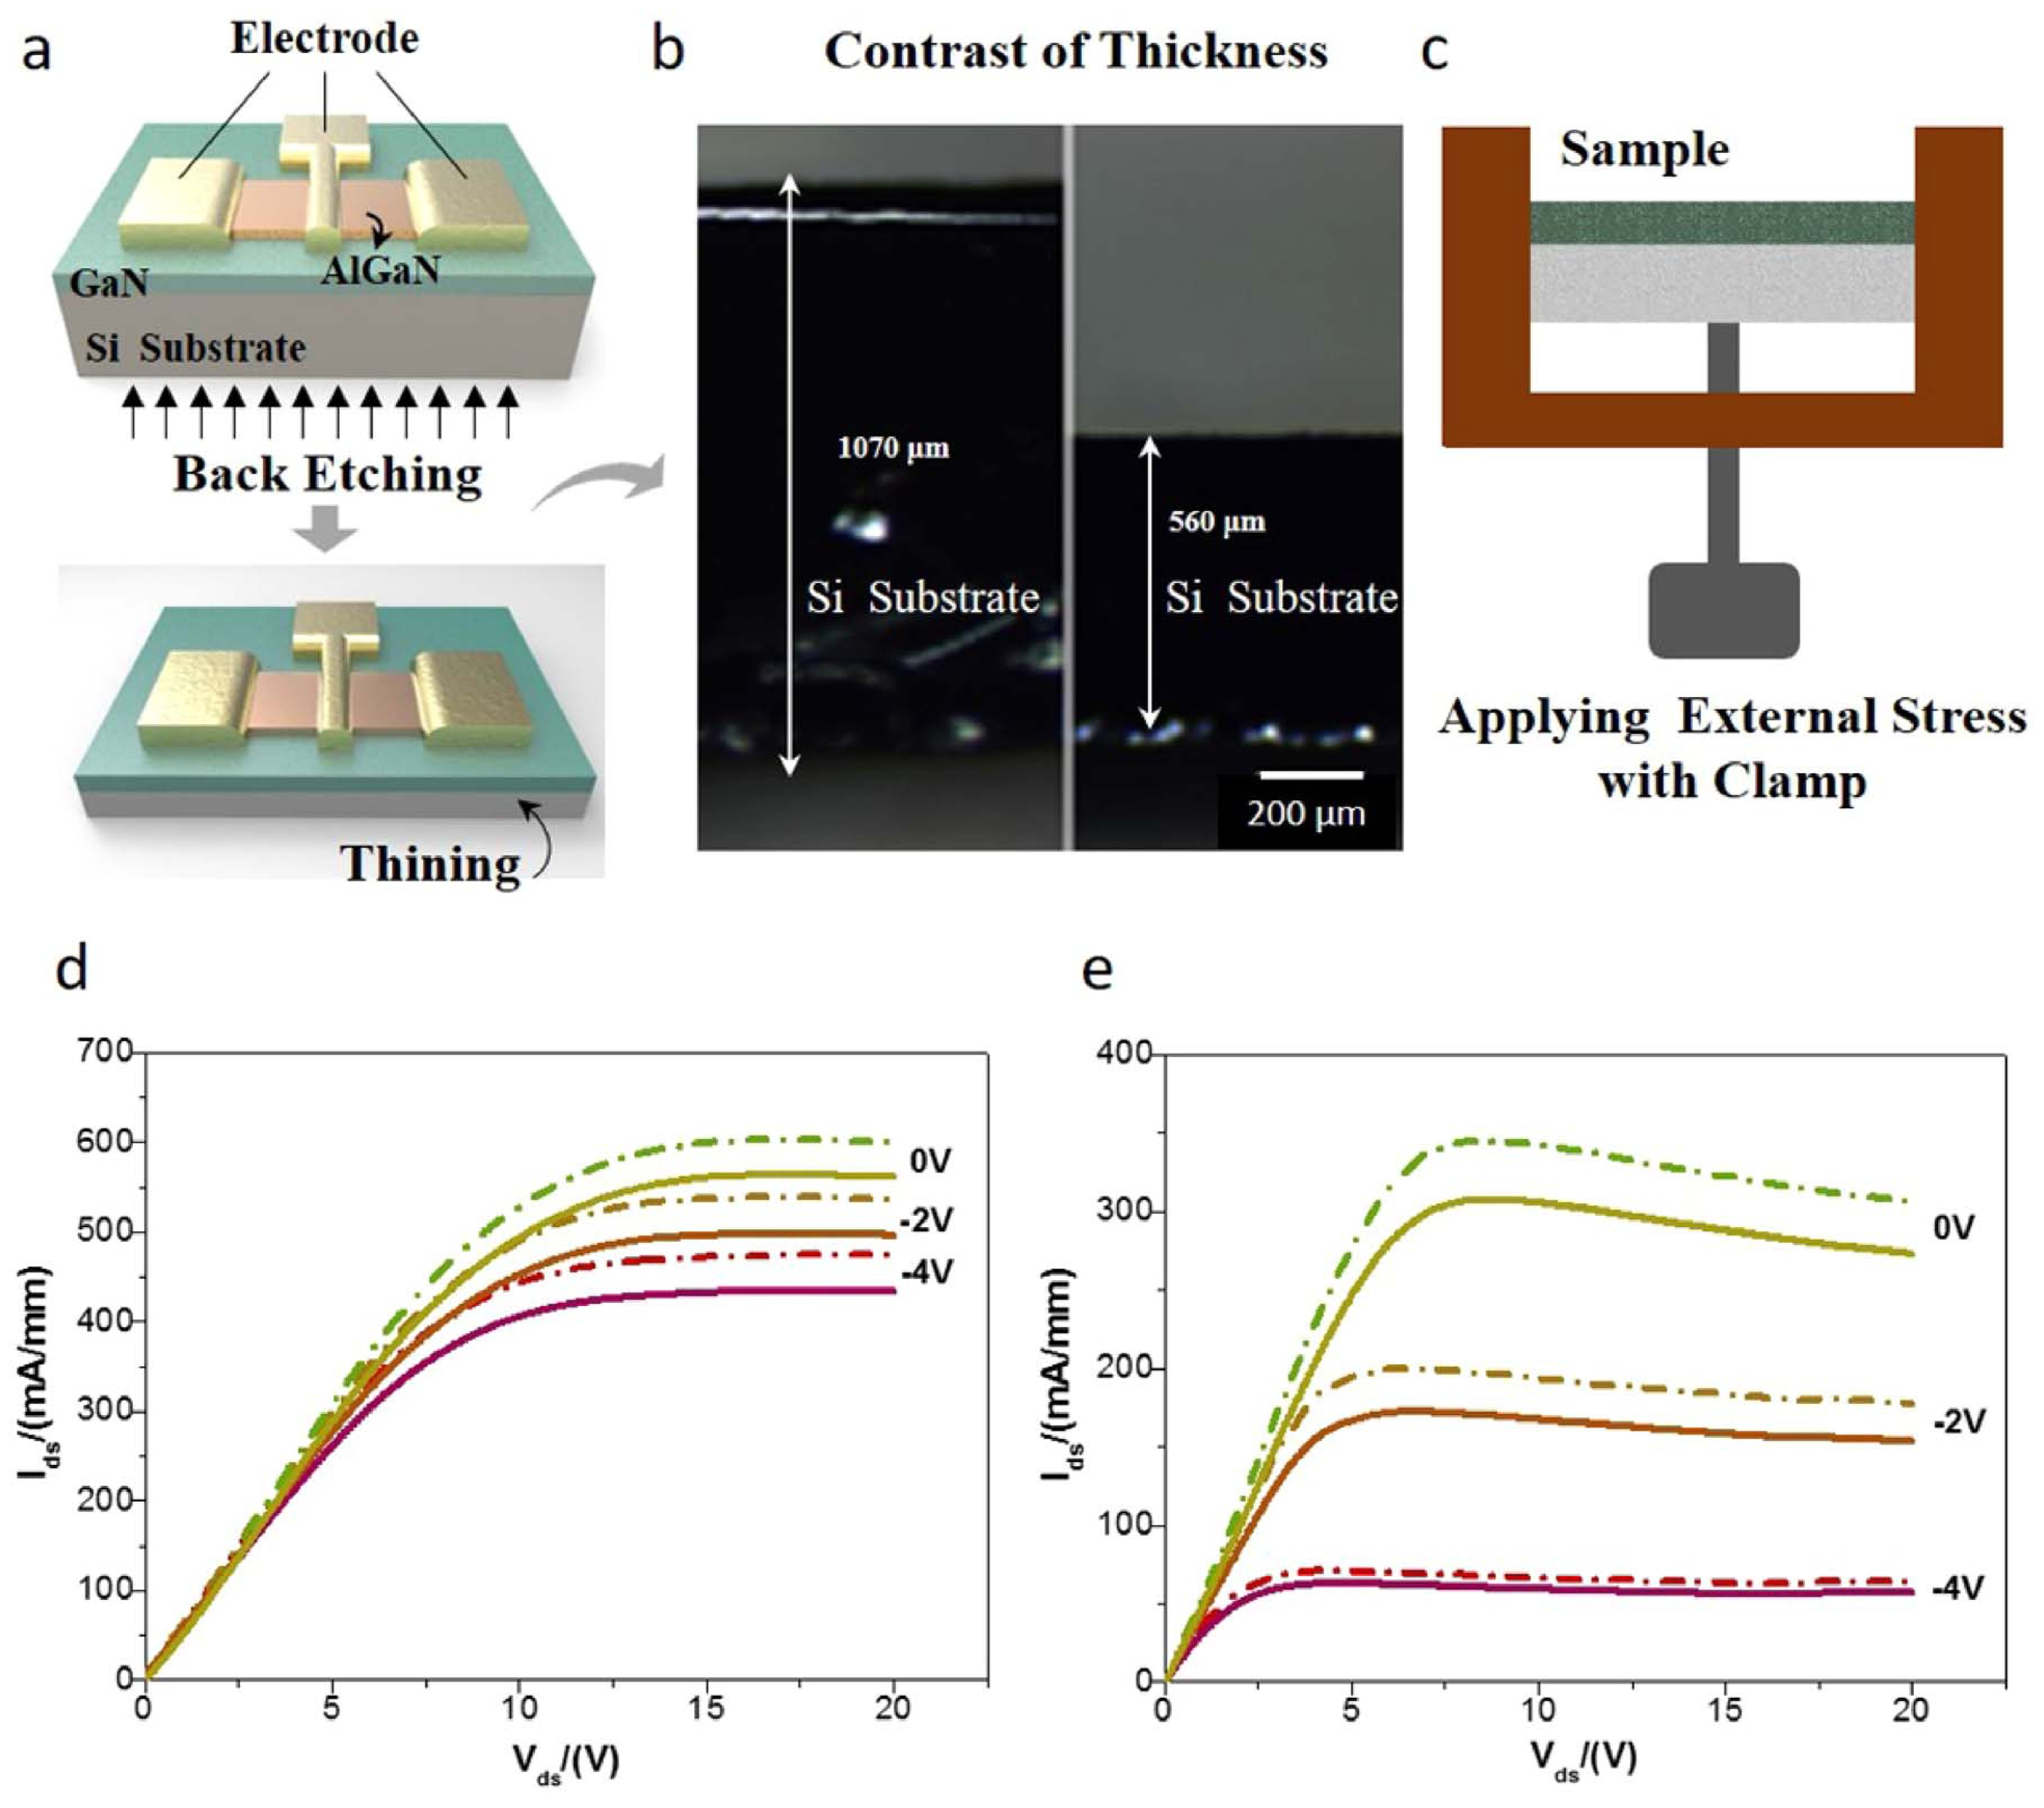
\includegraphics[width=0.9\textwidth]{ch1_10}
\caption[Piezotronics effect in AlGaN/GaN MOS HEMTs and unpassivated HEMTs]{Piezotronics effect in AlGaN/GaN MOS HEMTs and unpassivated HEMTs \protect\cite{liu2017electrical}}
\label{fig:1.10}
\end{figure}

Flexible electronics have received increasing attention due to their wide-ranging applications in fields such as healthcare, robotics, and artificial intelligence. Based on the work of Liu et al., Zhu et al. successfully fabricated flexible AlGaN/GaN HEMTs \index{HEMT} and studied their electrical properties under bending strain \index{Strain} through piezotronics \index{Piezotronics} effects (\autoref{fig:1.11}) \cite{zhu2019piezotronic,zhu2020thesis}. 

\begin{figure}[H] 
\centering    
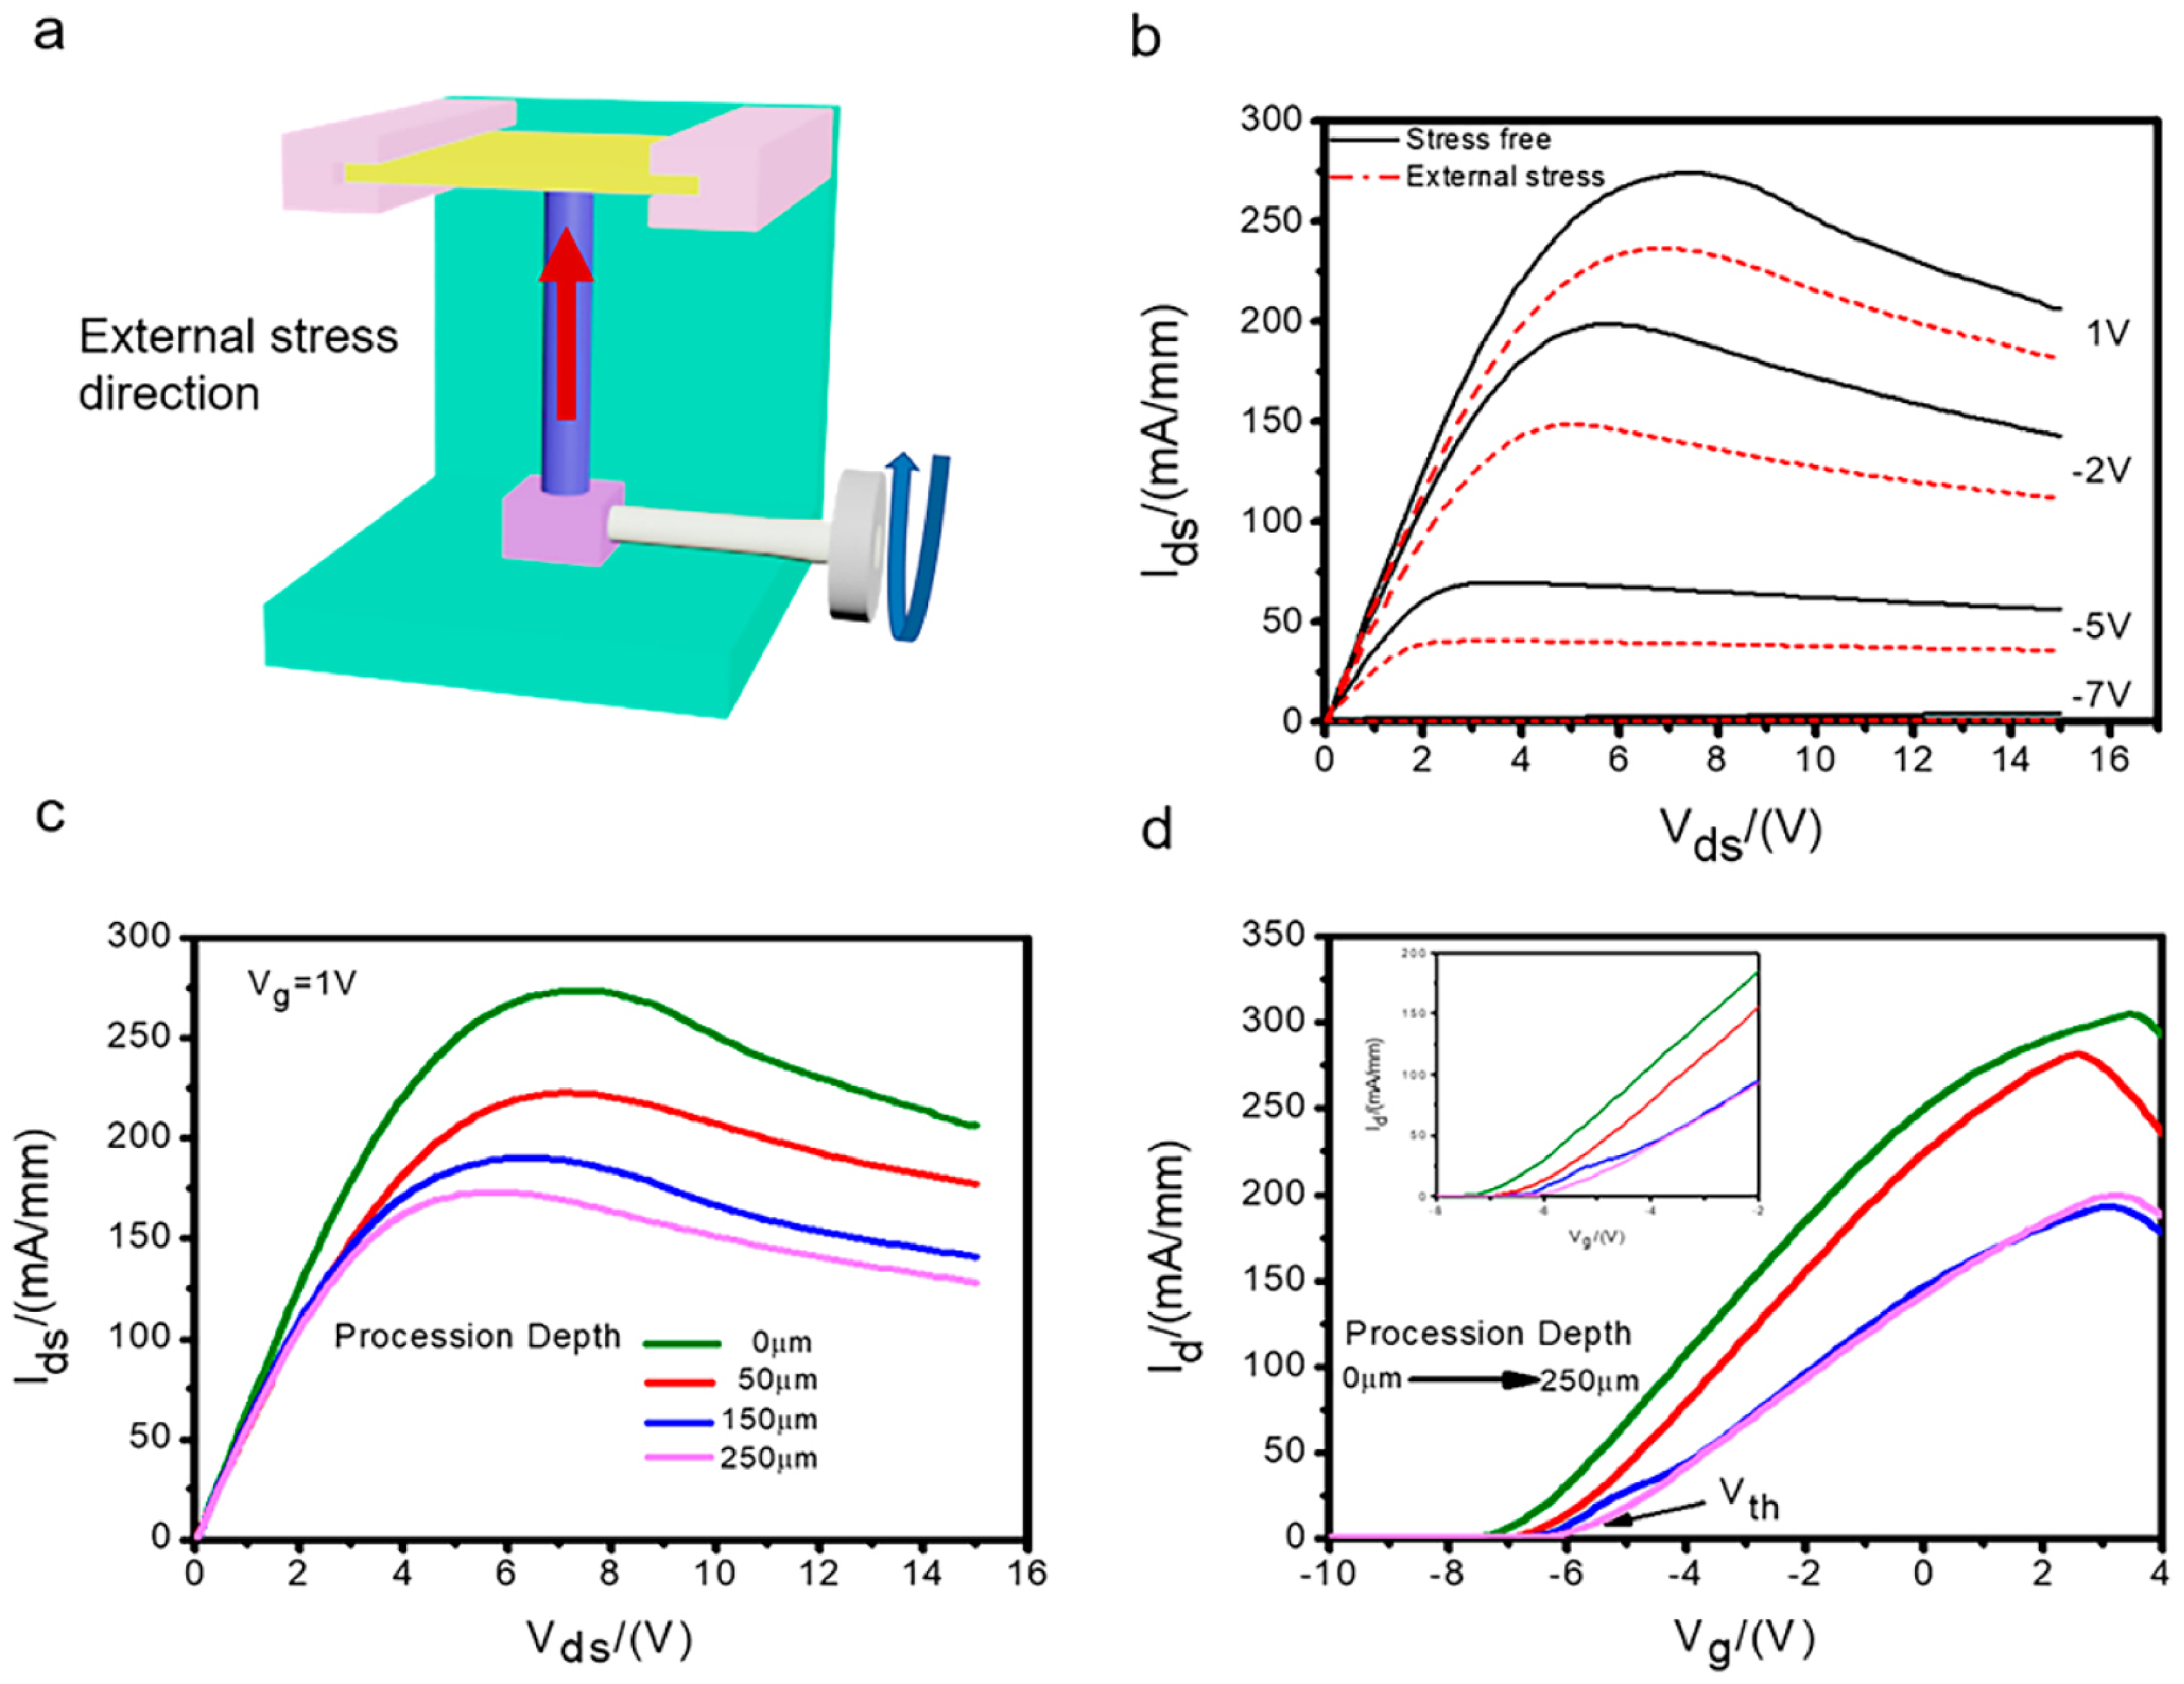
\includegraphics[width=0.9\textwidth]{ch1_11}
\caption[Piezotronics effect modulated flexible AlGaN/GaN HEMT]{Piezotronics effect modulated flexible AlGaN/GaN HEMT \protect\cite{zhu2019piezotronic}}
\label{fig:1.11}
\end{figure}

\noindent The fabricated flexible AlGaN/GaN HEMT \index{HEMT} completely removes the rigid silicon substrate \index{Substrate} and has excellent electrical properties. When the gate voltage \index{Voltage!gate voltage} $V_{gs}$ = \SI{2}{\volt}, the maximum saturated drain current \index{Current!drain current} density $I_{ds,max}$ reaches 290 \unit{\mA\per\mm}, The maximum transconductance \index{Transconductance} $g_{m, max}$ reaches 40 \unit{\milli\siemens\per\mm}. At the same time, the flexible HEMT can withstand large bending \index{Strain} strains. Based on the piezotronics \index{Piezotronics} effect of the AlGaN/GaN heterojunction, mechanical stress was introduced in the experiment to study the electrical properties of the flexible HEMT under strain. The results show that the output current \index{Output!current} of the flexible HEMT \index{HEMT} device can be significantly modulated \index{Modulation} by the external strain, and the electrical performance of the device will be degraded \index{Degradation} if it is subjected to forward bending \index{Strain} strain. Flexible HEMT devices modulated by piezotronics effects \index{Piezotronics} have broad application prospects in the fields of wearable electronics, smart \index{MEMS} MEMS, and human-computer interaction.


%********************************** % Third Section  *************************************
\section{Introduction to III-V nitride MEMS devices}  %Section - 1.3 

\subsection{Introduction to micro-electromechanical systems (MEMS)}

In the past decade, Micro-electromechanical systems (MEMS) \index{MEMS} technology has developed from a basic exploratory research to an important mainstream technology that has been widely used in many fields \cite{lyshevski2018nano,hsumems,gardner2003microsensors}. As an industrial technology that integrates microelectronics technology and mechanical engineering, MEMS combines the electrical information processing function and the mechanical sensing function to form a micro-electromechanical integrated system. MEMS have three main characteristics:

\begin{itemize}
	\item [1)] Combines electrical and mechanical components in order to sense its environment (mechanical sensors).
	\item [2)] Ability to analyze data (electronics) and react to changes in the environment (actuators).
	\item [3)] Devices are typically fabricated by microelectronics and have dimensions on the order of micrometers to millimeters.
\end{itemize}

Therefore, MEMS can "perceive", "think" and "react", and it is an intelligent micro-integrated system. The system block diagram of MEMS is shown in \autoref{fig:1.12}.

\begin{figure}[H] 
\centering    
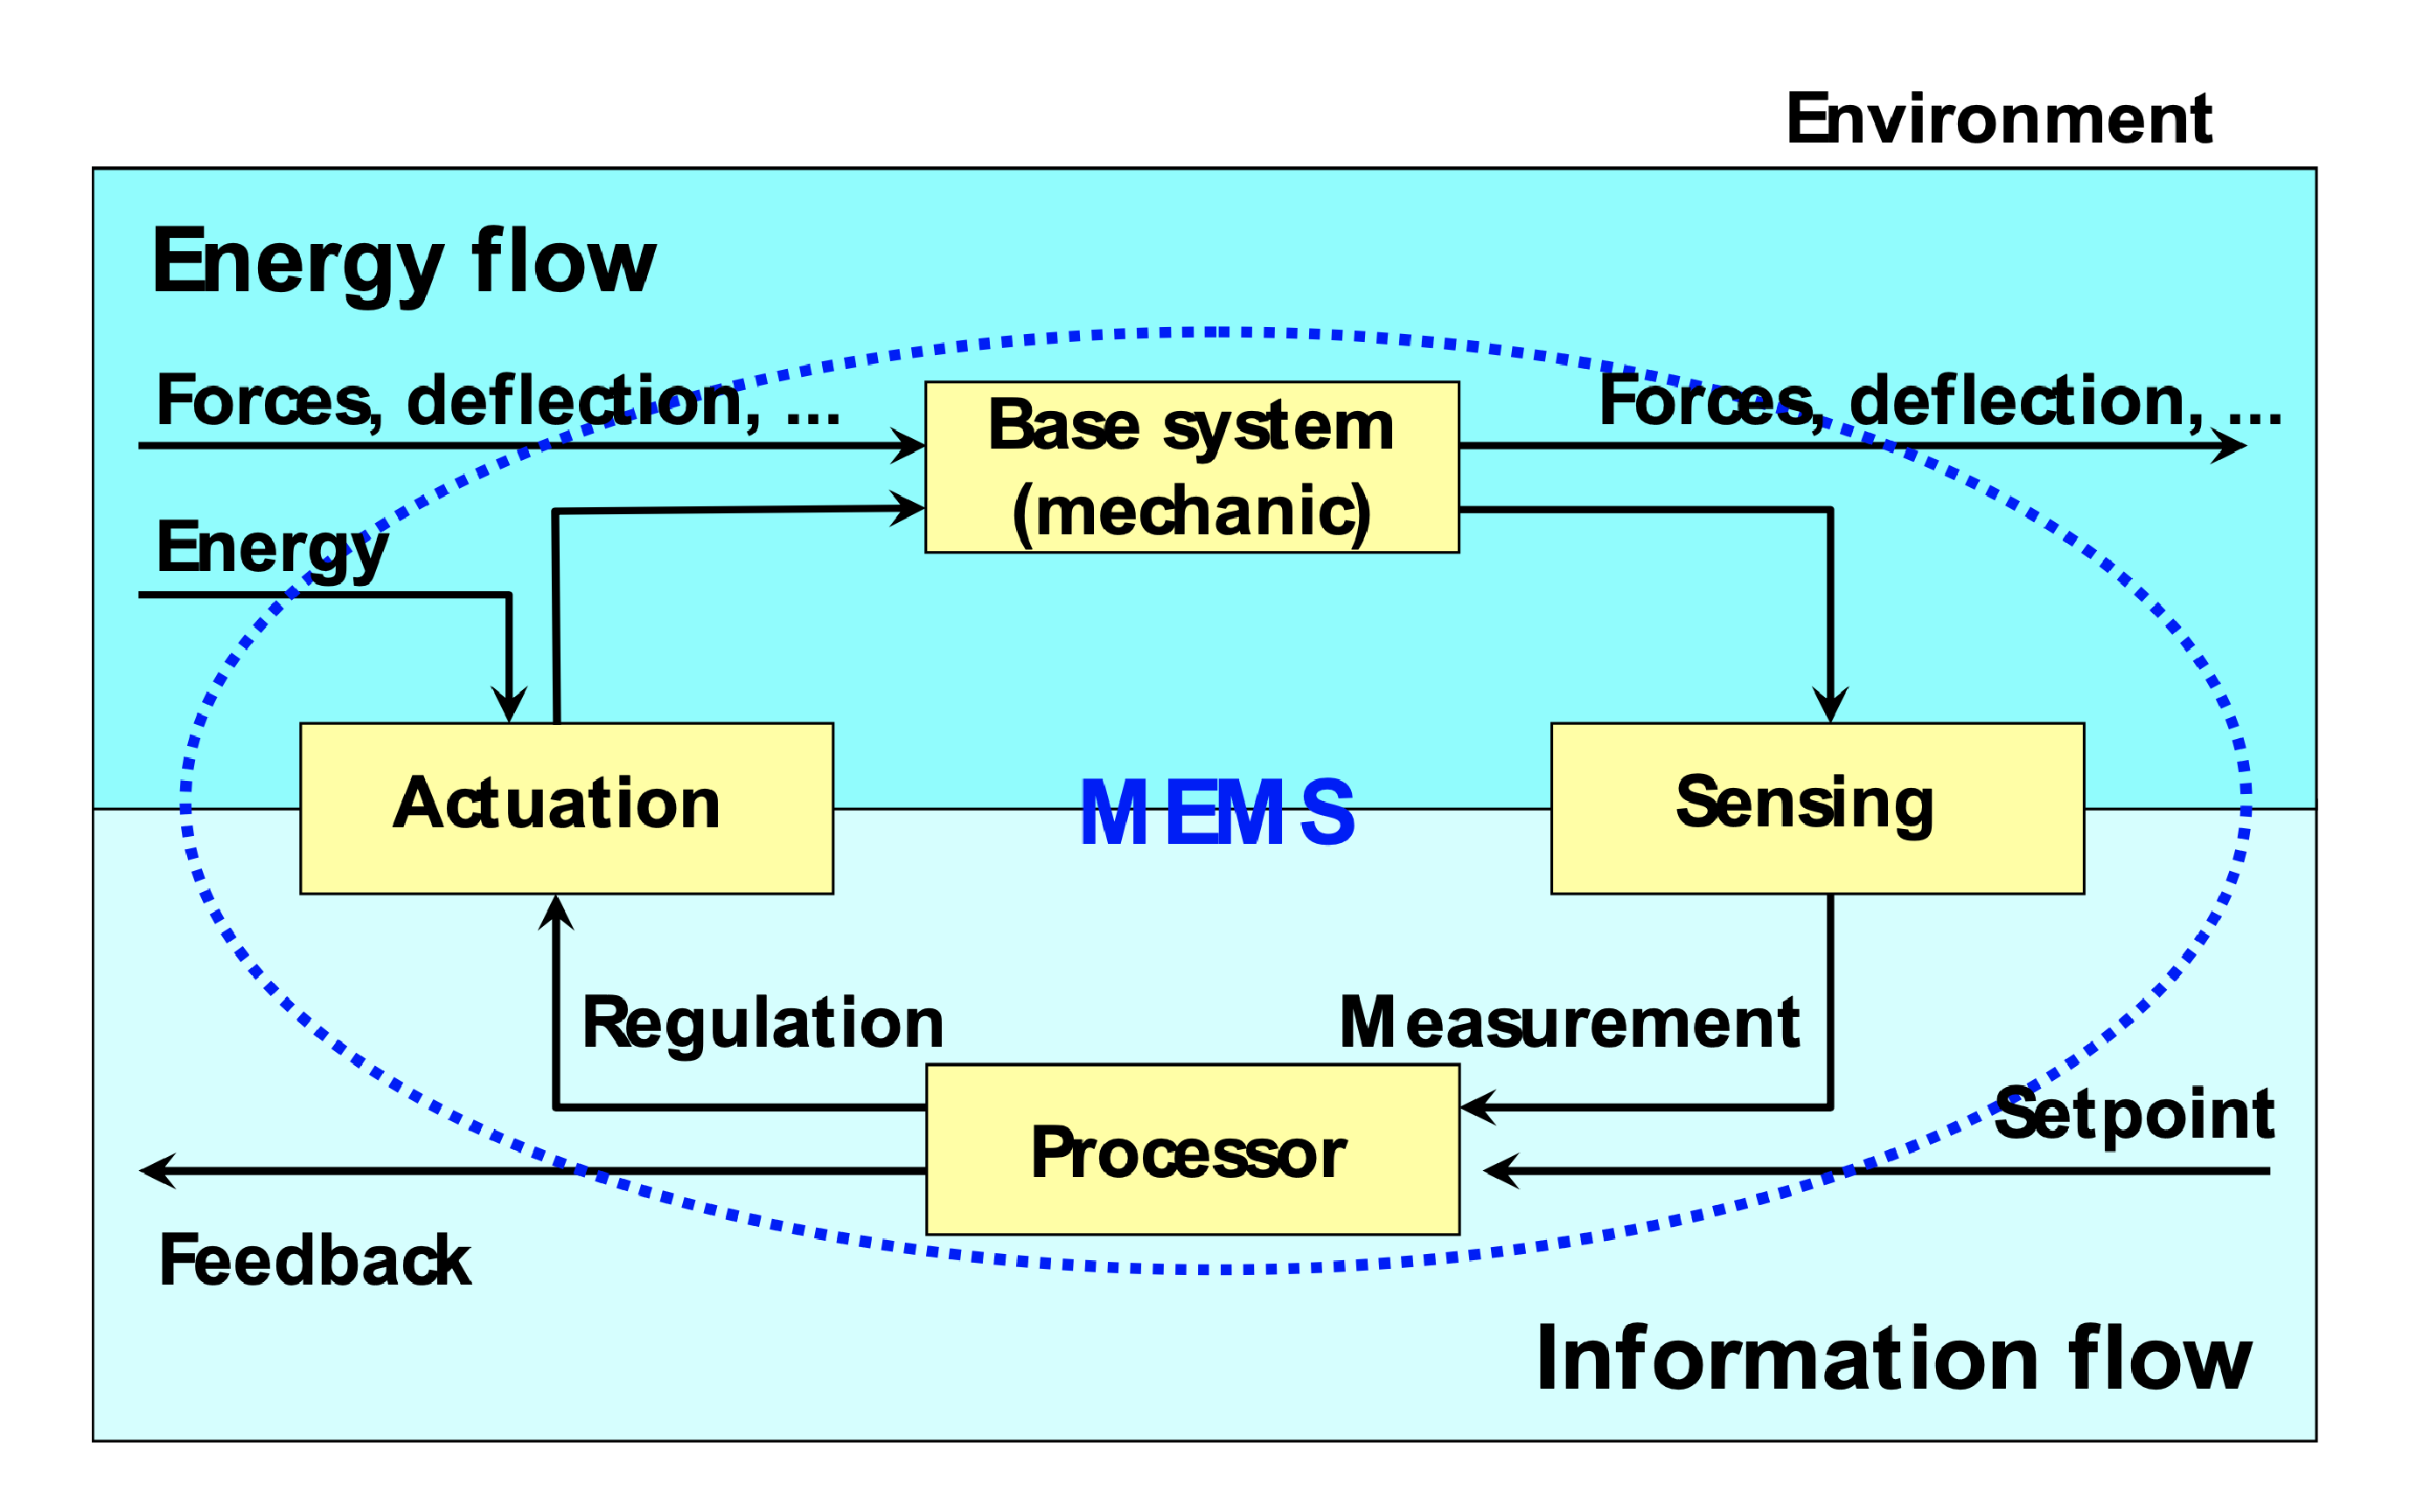
\includegraphics[width=0.9\textwidth]{ch1_12}
\caption[Block diagram for the basic components in MEMS and their interaction]{Block diagram for the basic components in MEMS and their interaction \protect\cite{cimalla2010algan}}
\label{fig:1.12}
\end{figure}


\subsection{III-V nitride MEMS devices}

With the rapid development of silicon-based microelectronics technology, the integration of Si-based MEMS \index{MEMS} devices has rapidly increased, and the system's "response" is faster, more reliable, cheaper, and capable of incorporating more complex functions. Si-based MEMS devices are being used in more and more fields \cite{ciuti2015mems}, including chemical, biological and physical sensors \cite{yabuki2014heat,wang2004ultra,khoshnoud2012recent-a,khoshnoud2012recent-b}, microfluidic sensors \cite{kottapalli2011liquid}, radio frequency MEMS \cite{fernandez2006capacitive,donelli2018exploitation}, micro-opto-electro-mechanical system (MOEMS) \cite{lee2008development,iannacci2018internet}, Internet of Things, etc., as well as various MEMS-based acceleration, pressure, and flow sensors \cite{davidson2008using,marek2011automotive,berndt2020mems} used in the automotive industry. However, Si-based MEMS have shown limitations for sensing in harsh environmental conditions \cite{french2016precision}, an issue that has received increasing attention over the past few years. First, Si-based MEMS cannot be used for high-temperature applications because Si materials lose mechanical reliability at \SI{500}{\degreeCelsius} \cite{french2016precision}. Second, Si materials are easily attacked by corrosive media and have low biochemical compatibility, which limits its application in the field of biosensing \cite{french2016precision}. Therefore, additional protection of the sensing and actuation elements is necessary for chemical and biological Si-based MEMS sensors, which are generally no longer integrated systems. For these reasons, Si-based MEMS allow only very limited applications. These shortcomings of Si-based MEMS technology have stimulated research into MEMS of more biochemically resistant and thermally stable materials such as wide-bandgap semiconductors.

\begin{table}[H]
\renewcommand\arraystretch{1.2}
\centering
\caption[Comparison of characteristics of several electromechanical materials]{Comparison of characteristics of several electromechanical materials \protect\cite{rais2014gallium}}
\begin{tabular}{ccccccc}
\hline
\hline
Material &
  \begin{tabular}[c]{@{}c@{}}Elastic \\Modulus $C33$ \\ (\unit{GPa})\end{tabular} &
  \begin{tabular}[c]{@{}c@{}}Acoustic \\Velocity\\  (\unit{m/s})\end{tabular} &
  \begin{tabular}[c]{@{}c@{}}Piezoelectric \\Coefficient $e33$ \\ (\unit{\coulomb\per\square\m})\end{tabular} &
  \begin{tabular}[c]{@{}c@{}}$f \times Q$ \\ (\unit{Hz}) \end{tabular} &
  \begin{tabular}[c]{@{}c@{}}$K_{eff}^{2}$ \\ (\%) \end{tabular} &
  Ref \\ \hline \hline
Si   & 165 & 8415  & N/A   & \num{2.5e13}   & N/A  & \cite{tabrizian2009effect}       \\
SiC  & 605 & 13100 & 0.2   & \num{3.5e14}   & 0.08 & \cite{tabrizian2009effect,karmann1989piezoelectric,shur1996handbook,shur2006sic}    \\
GaAs & 118 & 2470  & -0.16 & --                     & 0.04 & \cite{adachi1992physical,adachi1994gaas}    \\
AlN  & 390 & 11000 & 1.55  & \num{e13}              & 5.6  & \cite{tabrizian2009effect,zou2010high}    \\
GaN  & 398 & 8044  & 0.65  & \num{5.0e12}     & 2    & \cite{tabrizian2009effect,gokhale2014phonon,gokhale2010observation,gokhale2011high,popa2014band} \\ \hline \hline
\end{tabular}
\label{tab:1.1}
\end{table}

III-V nitride \index{Nitride} materials are the main representatives of wide-bandgap semiconductors because of unique material properties that exhibit excellent mechanical, electrical, and perceptual properties in \index{MEMS} MEMS applications (\autoref{fig:1.13}) \cite{rais2014gallium,strittmatter2004development,cimalla2007group}. Compared to Si \cite{ekinci2005nanoelectromechanical}, the high Young's modulus \index{Young's modulus} of III-V nitrides \index{Nitride} enables higher frequencies and quality factor in resonant devices of the same geometry (\autoref{tab:1.1}). In addition, materials with high Young's modulus can better maintain the linear relationship between applied load and induced \index{Strain} strain. Another major advantage of III-V nitrides is their very high mechanical, thermal, chemical and biological stability \cite{kuball1998thermal,cimalla2007algan}. They have no or very low reactivity with molecules in air, and can be applied in reliable environmental sensors. Therefore, III-V nitride materials are very suitable for MEMS \index{MEMS} or NEMS applications. Finally, due to the high frequency properties of III-V nitride materials, they can be combined or integrated into MEMS as amplifiers for radio frequency devices. It is worth mentioning that the piezoelectric effect \index{Piezoelectric!effect} offers completely new possibilities to integrate new functionalities into MEMS devices \cite{tadigadapa2009piezoelectric}. The AlGaN/GaN heterojunction interface \index{Interface} contains a high concentration of two-dimensional \index{Two-dimensional electron gas (2DEG)} electron gas (2DEG), which is extremely sensitive to both mechanical loading and chemical modifications of the surface, such as (i) the charge on the free, unpassivated gate \index{Surface} surface; (ii) mechanical stress that modulates \index{Modulation} the internal piezoelectric \index{Piezoelectric!potential} potential; and (iii) external fields such as magnetic fields \index{Magnetic!field} or electromagnetic radiation. Therefore it is widely used in biochemical sensors \cite{eickhoff2003electronics,pearton2004gan,chen2008low,chang2008co,guo2012ph,kang2005electrical,kokawa2006liquid}, pressure sensors \cite{kang2005capacitance,sun2020low}, cantilever \index{Cantilever} sensors \cite{zimmermann2006piezoelectric,khmyrova2009multi,vittoz2011analytical}, and many other novel sensors. Compared with Si-based MEMS, MEMS \index{MEMS} devices based on III-V nitrides \index{Nitride} have broader development prospects.

\begin{figure}[H] 
\centering    
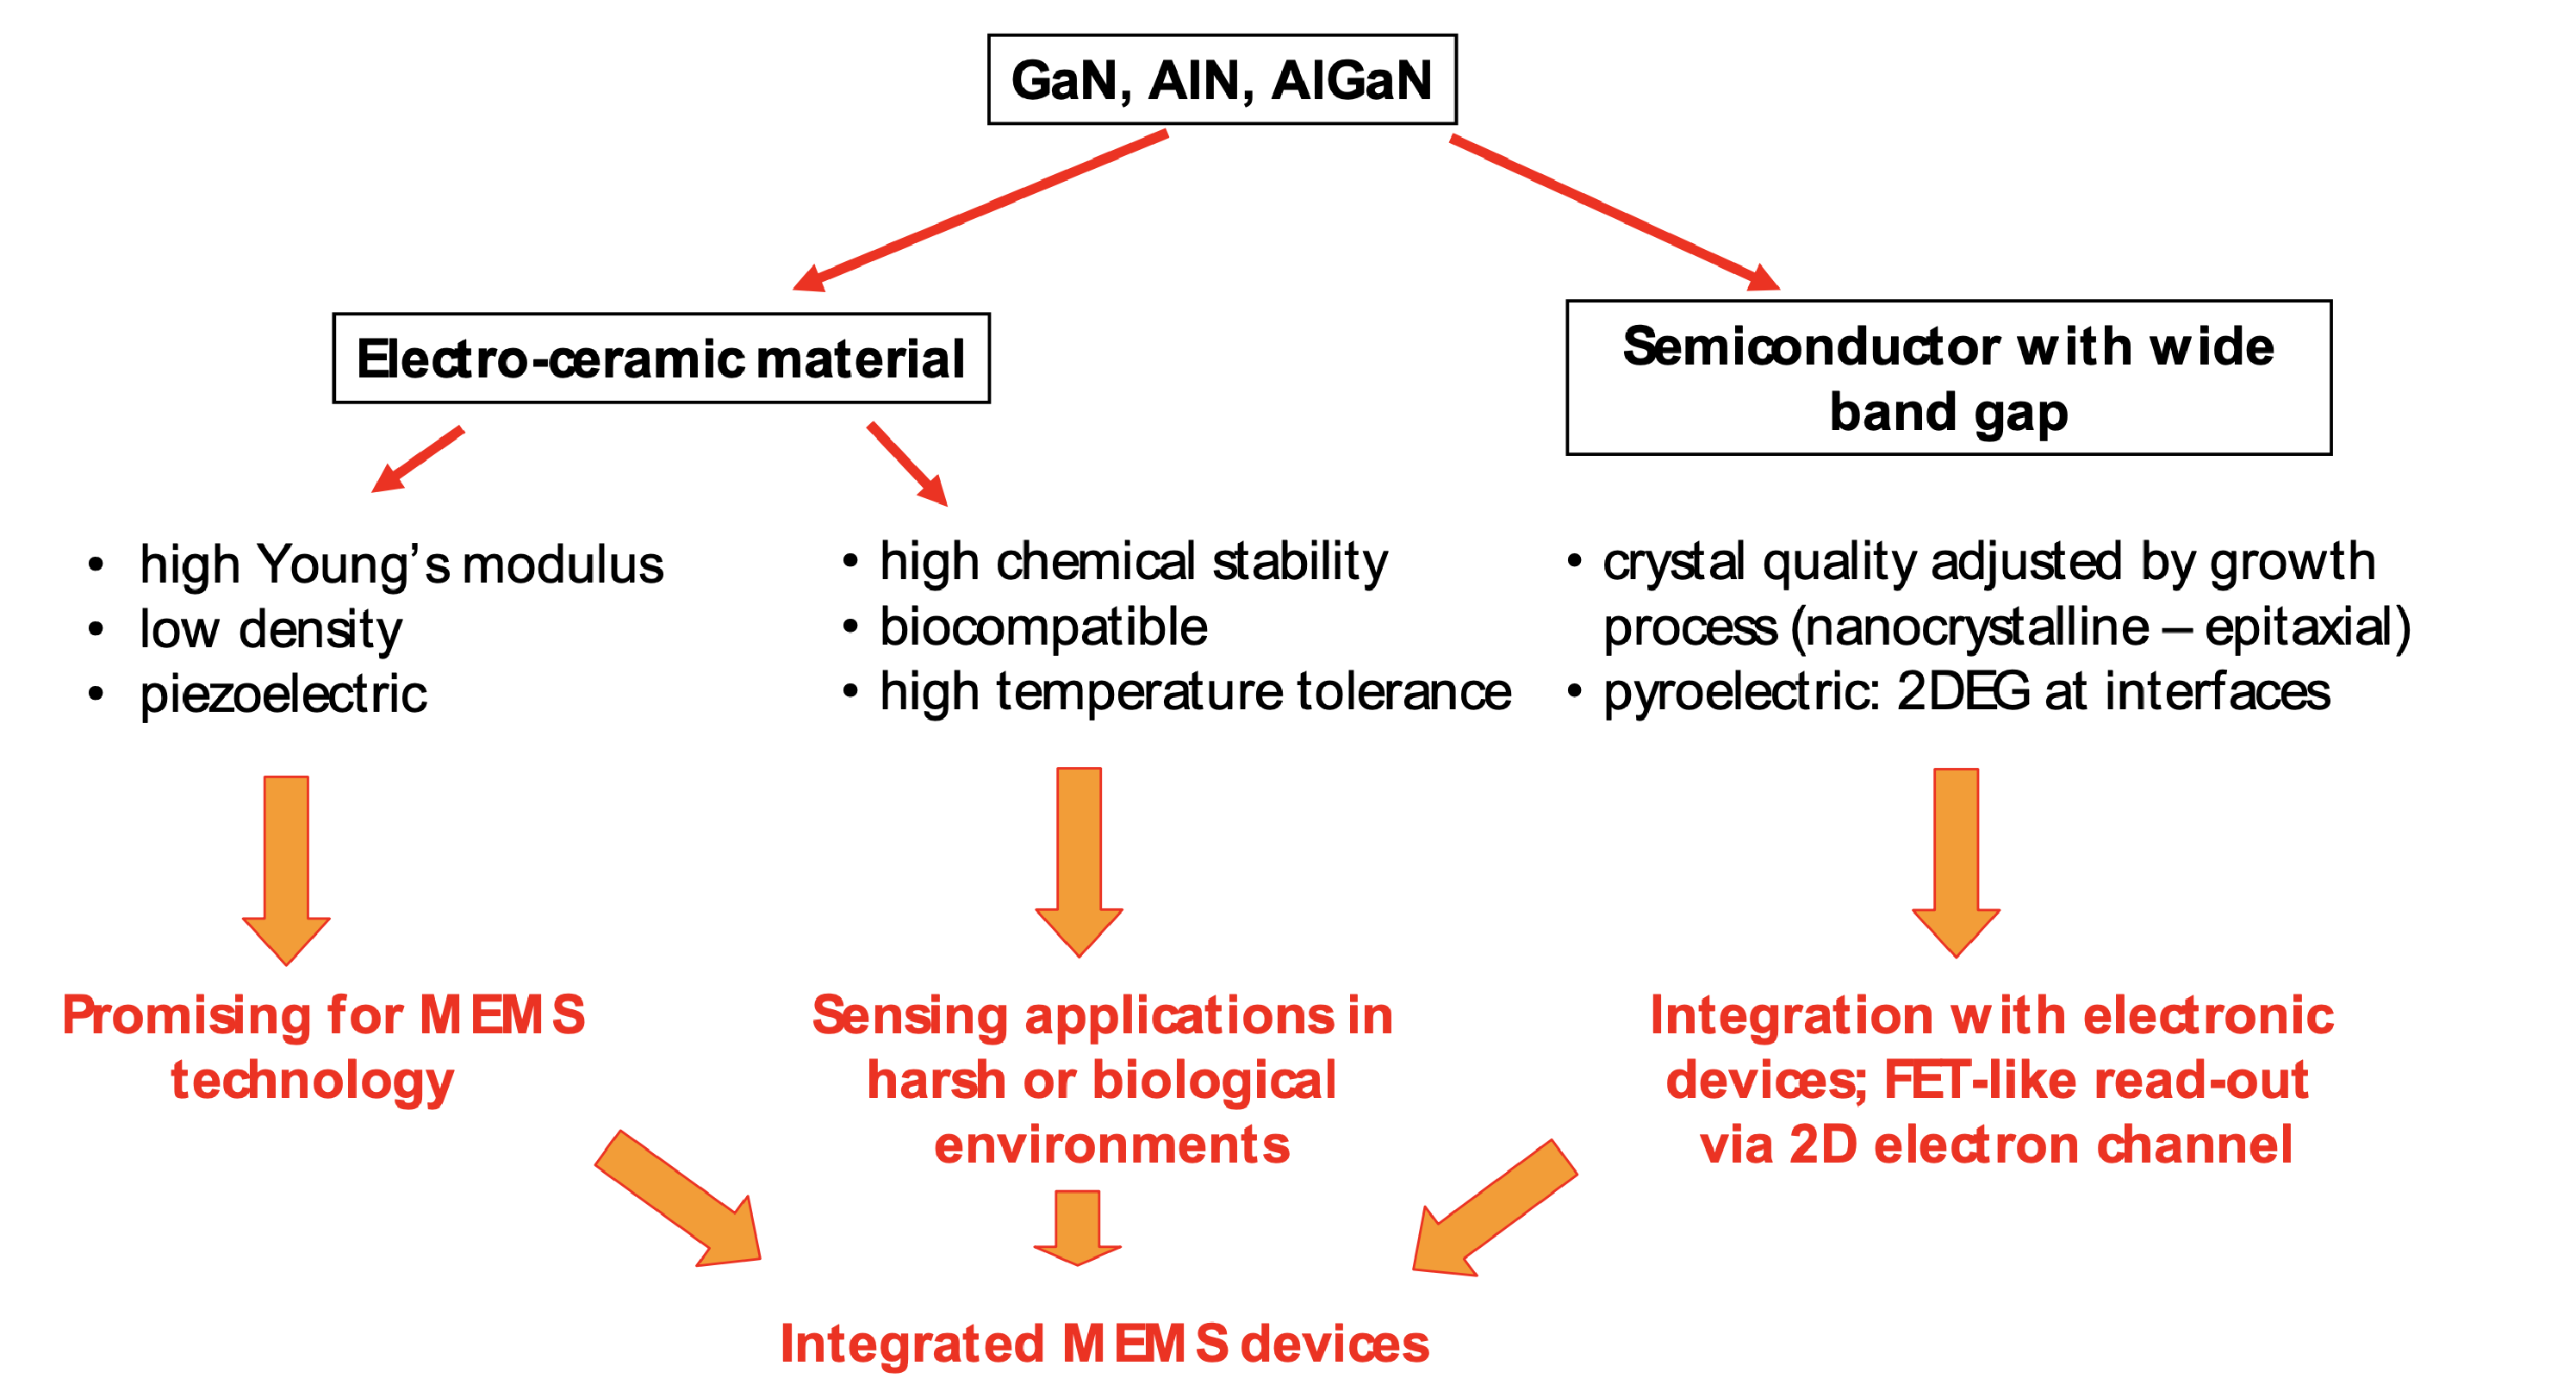
\includegraphics[width=0.9\textwidth]{ch1_13}
\caption[Advantages of group III-V nitrides for the realization of integrated MEMS]{Advantages of group III-V nitrides for the realization of integrated MEMS \protect\cite{cimalla2010algan}}
\label{fig:1.13}
\end{figure}

Based on the excellent properties of III-V nitride \index{Nitride} materials, the research on GaN-based MEMS \index{MEMS} devices has made remarkable progress. Azadeh Ansari et al. reported a gigahertz AlGaN/GaN resonant body transistor (RBT) \index{Resonant body transistor (RBT)} in which mechanical resonance and electrical signals can be modulated \index{Modulation} simultaneously, as shown in \autoref{fig:1.14} \cite{ansari2014thickness}. An AlGaN layer with a thickness of 17.5 \unit{\nm} was used as the piezoelectric transducer layer, and the 2DEG \index{Two-dimensional electron gas (2DEG)} at the AlGaN/GaN interface \index{Interface} was used as the bottom electrode \index{Electrode} as well as the transistor conduction \index{Channel} channel. The strain \index{Strain} generated by the acoustic wave can effectively modulate the 2DEG concentration \index{Two-dimensional electron gas (2DEG)} of the \index{Channel} channel. A quality factor of 250 and an acoustic transconductance \index{Transconductance} of 25 \unit{\micro\siemens} are obtained at the resonant frequency of 4.23 \unit{\GHz}, resulting in excellent mechanical and electrical properties.

\begin{figure}[H] 
\centering    
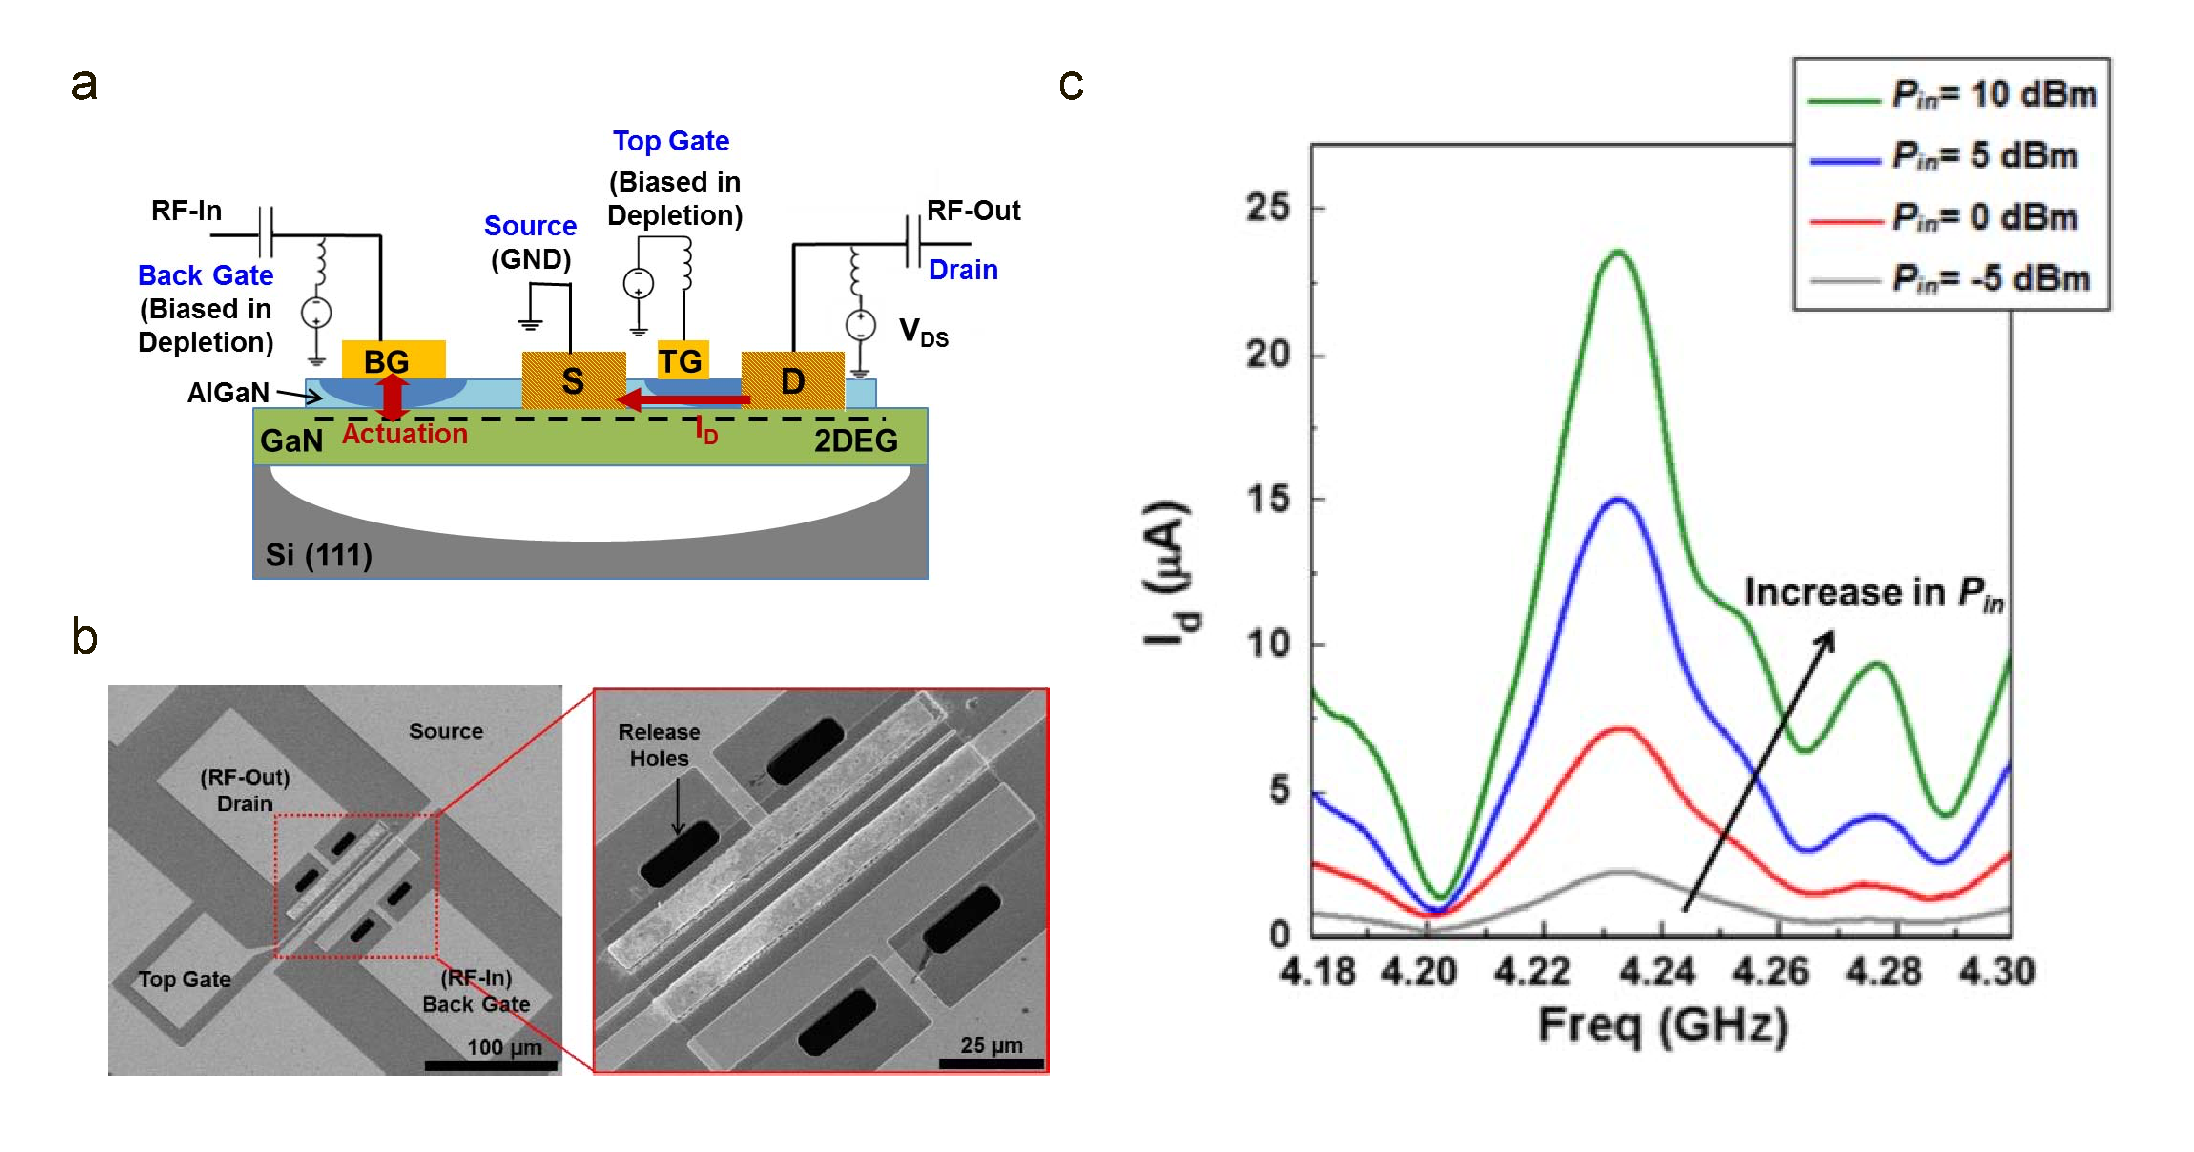
\includegraphics[width=0.9\textwidth]{ch1_14}
\caption[The AlGaN/GaN resonant body high electron mobility transistor]{The AlGaN/GaN resonant body high electron mobility transistor \protect\cite{ansari2014thickness}}
\label{fig:1.14}
\end{figure}

The development of all-GaN integrated \index{MEMS} MEMS has always been the focus of research in the field of GaN-based MEMS. On the basis of the above work, Azadeh Ansari et al. reported an all-GaN integrated microsystem platform integrating high-frequency GaN-based MEMS resonators and AlGaN/GaN HEMTs, as shown in \autoref{fig:1.15} \cite{ansari2012monolithic}. For the first time, stacked high-quality GaN bulk acoustic resonators and AlGaN/GaN \index{HEMT} HEMTs have been fabricated on \index{Substrate} silicon substrates, achieving signal tuning over 30 \unit{\dB} using HEMT \index{HEMT} amplifiers. This work can serve as a starting point for further development of integrated GaN-based MEMS, that is, integrating GaN-based devices (MEMS, HEMT, RBT, etc.) together to build fully GaN integrated MEMS with different architectures and functions.

\begin{figure}[H] 
\centering    
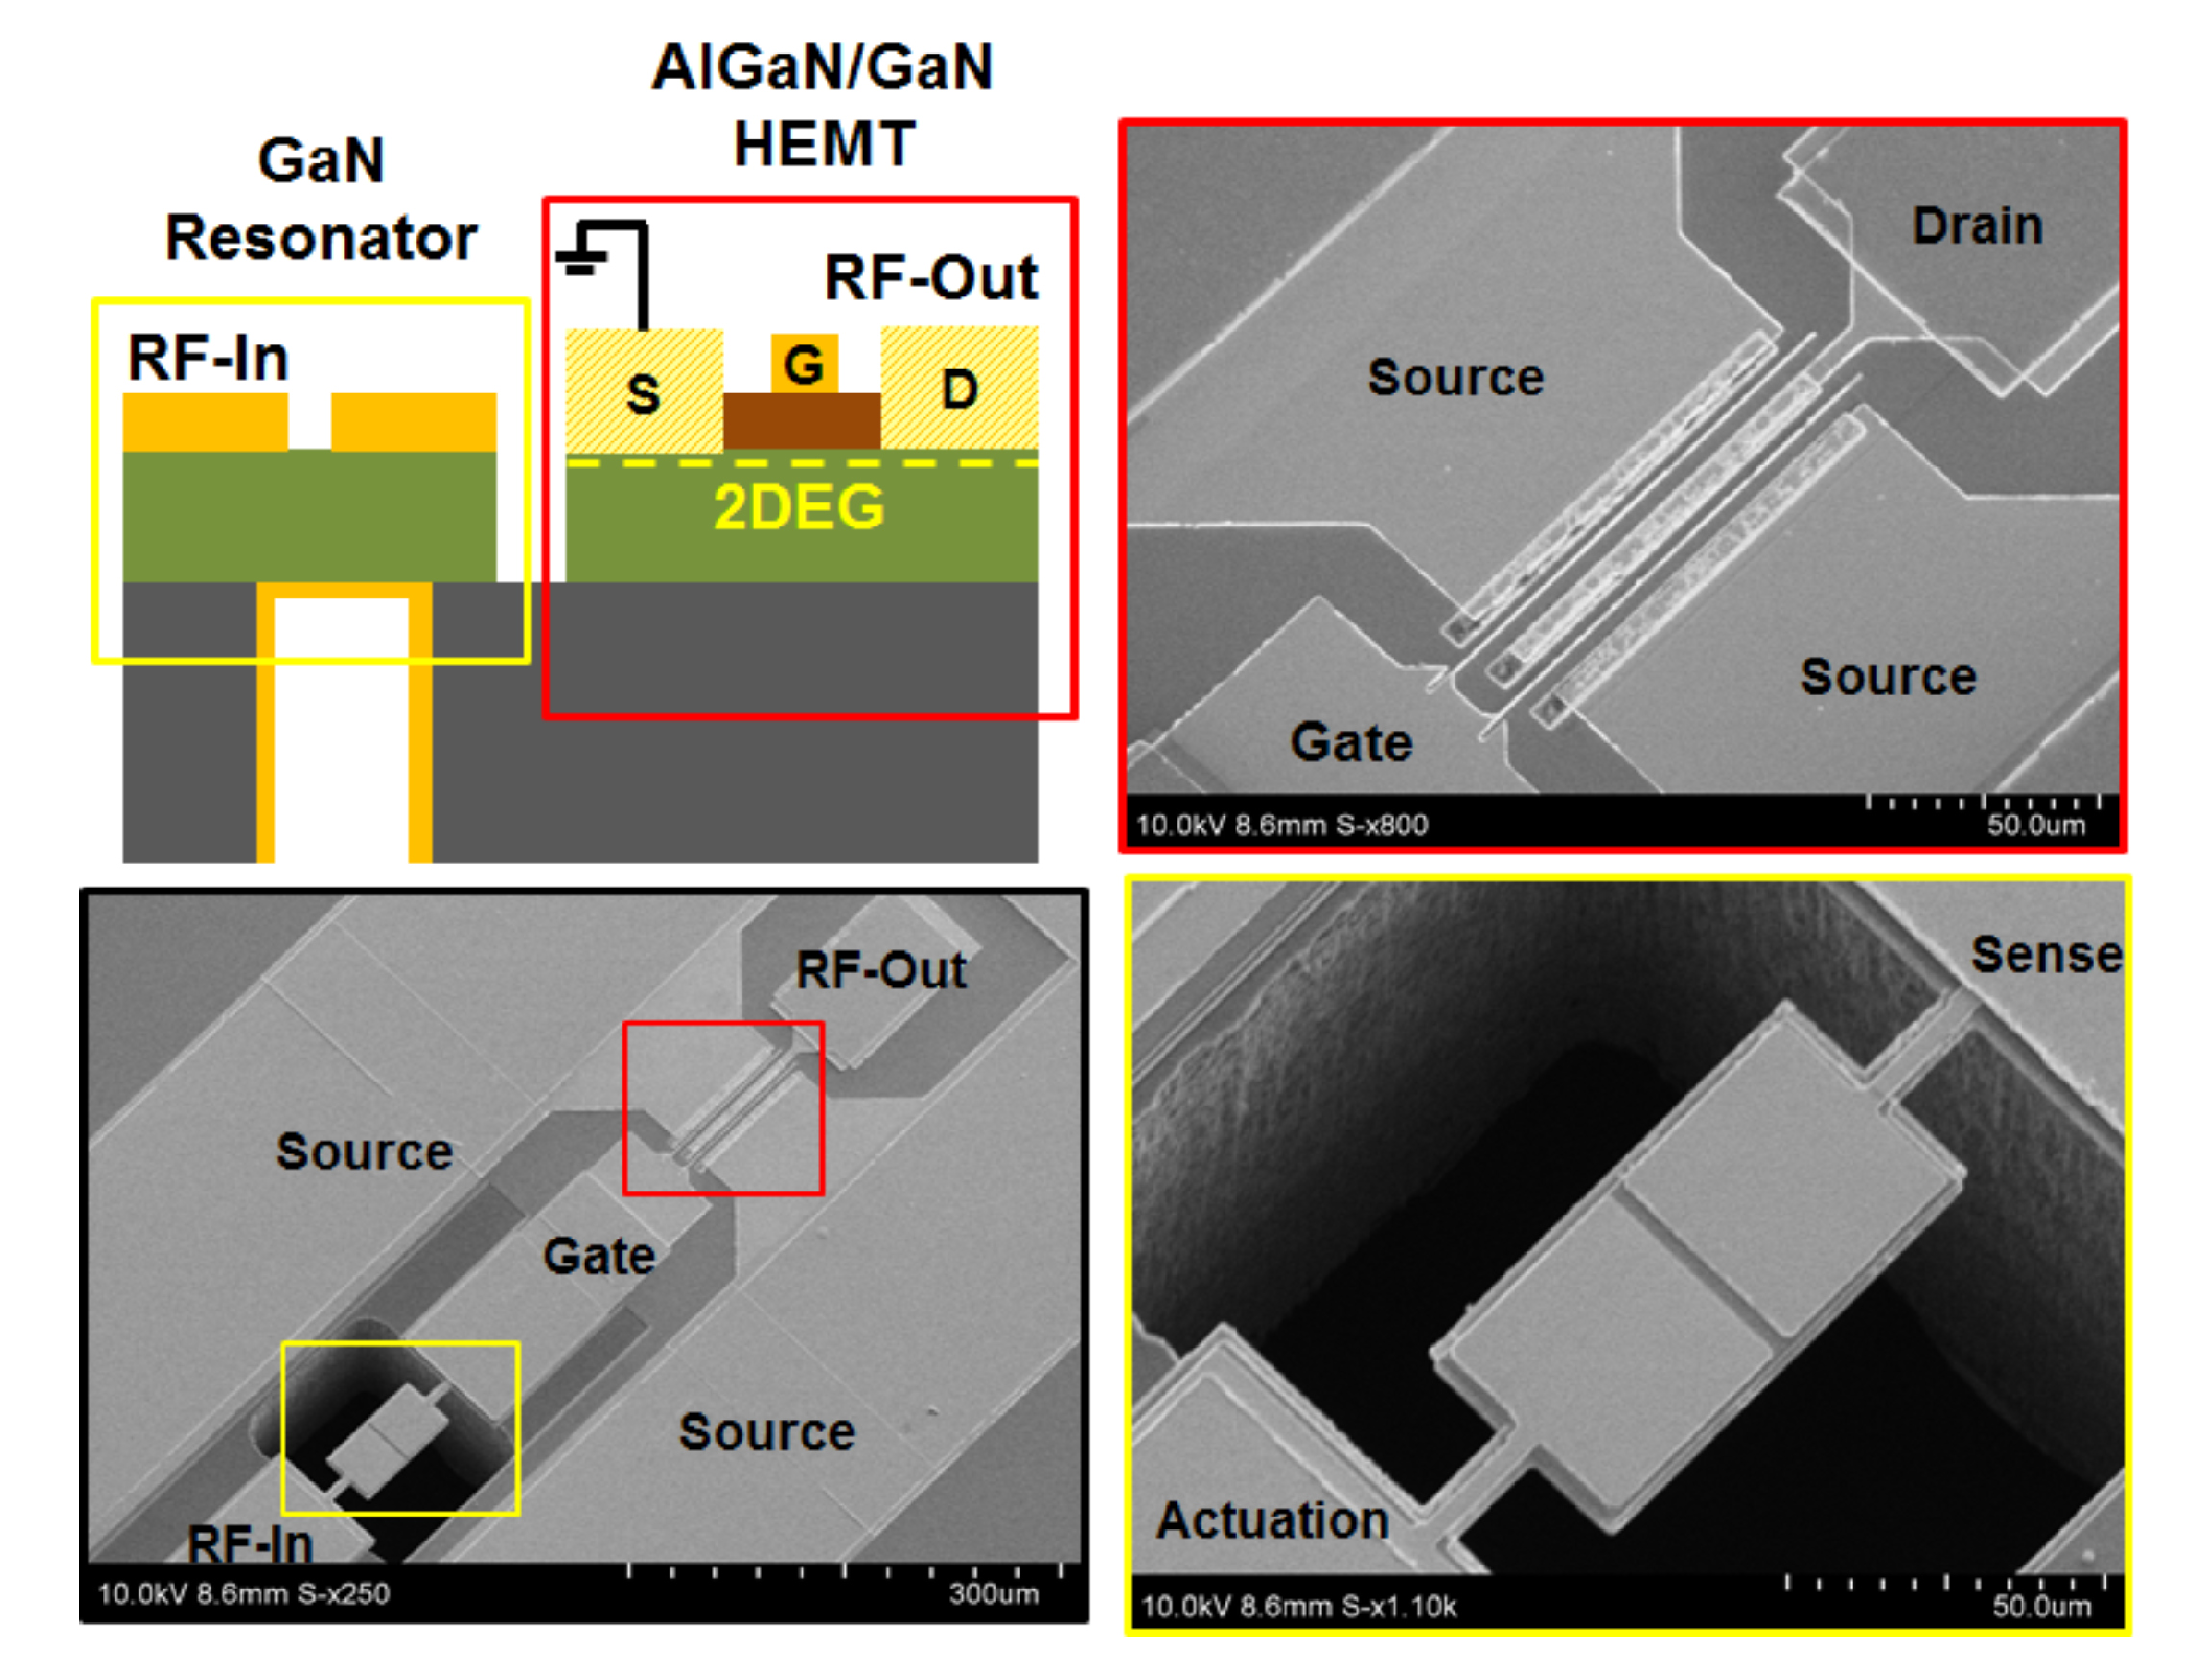
\includegraphics[width=0.9\textwidth]{ch1_15}
\caption[An all-GaN integrated microsystem platform wherein GaN MEMS resonators are monolithically integrated with AlGaN/GaN HEMT]{An all-GaN integrated microsystem platform wherein GaN MEMS resonators are monolithically integrated with AlGaN/GaN HEMT \protect\cite{ansari2012monolithic}}
\label{fig:1.15}
\end{figure}

Based on the unique piezoelectric effect \index{Piezoelectric!effect} of III-V nitride \index{Nitride} materials, Sun et al. reported a miniature pressure MEMS \index{MEMS} sensor based on a suspended structure of AlGaN/GaN heterojunction (\autoref{fig:1.16}) \cite{sun2020low}. The sensor's drain current \index{Current!drain current} can respond quickly when subjected to different pressures (especially in the low pressure range below 600 \unit{Pa}). Under the operating condition of \SI{100}{\degreeCelsius}, the dynamic current change percentage of the sensor is 18.75$\%$ when the pressure is changed from 96 \unit{KPa} to 10 \unit{Pa}, and the power consumption is only 1.8 \unit{uW}. In the pressure range of 600 \unit{Pa} to 10 \unit{Pa}, the maximum sensitivity of the sensor is 22.8$\%$/\unit{KPa}. Meanwhile, at higher temperature, the thermally induced displacement of the film increases the 2DEG \index{Two-dimensional electron gas (2DEG)} concentration, and the drain current response of the sensor increases accordingly. Therefore, miniature pressure MEMS sensors can be applied to high vacuum and high temperature sensing.

\begin{figure}[H] 
\centering    
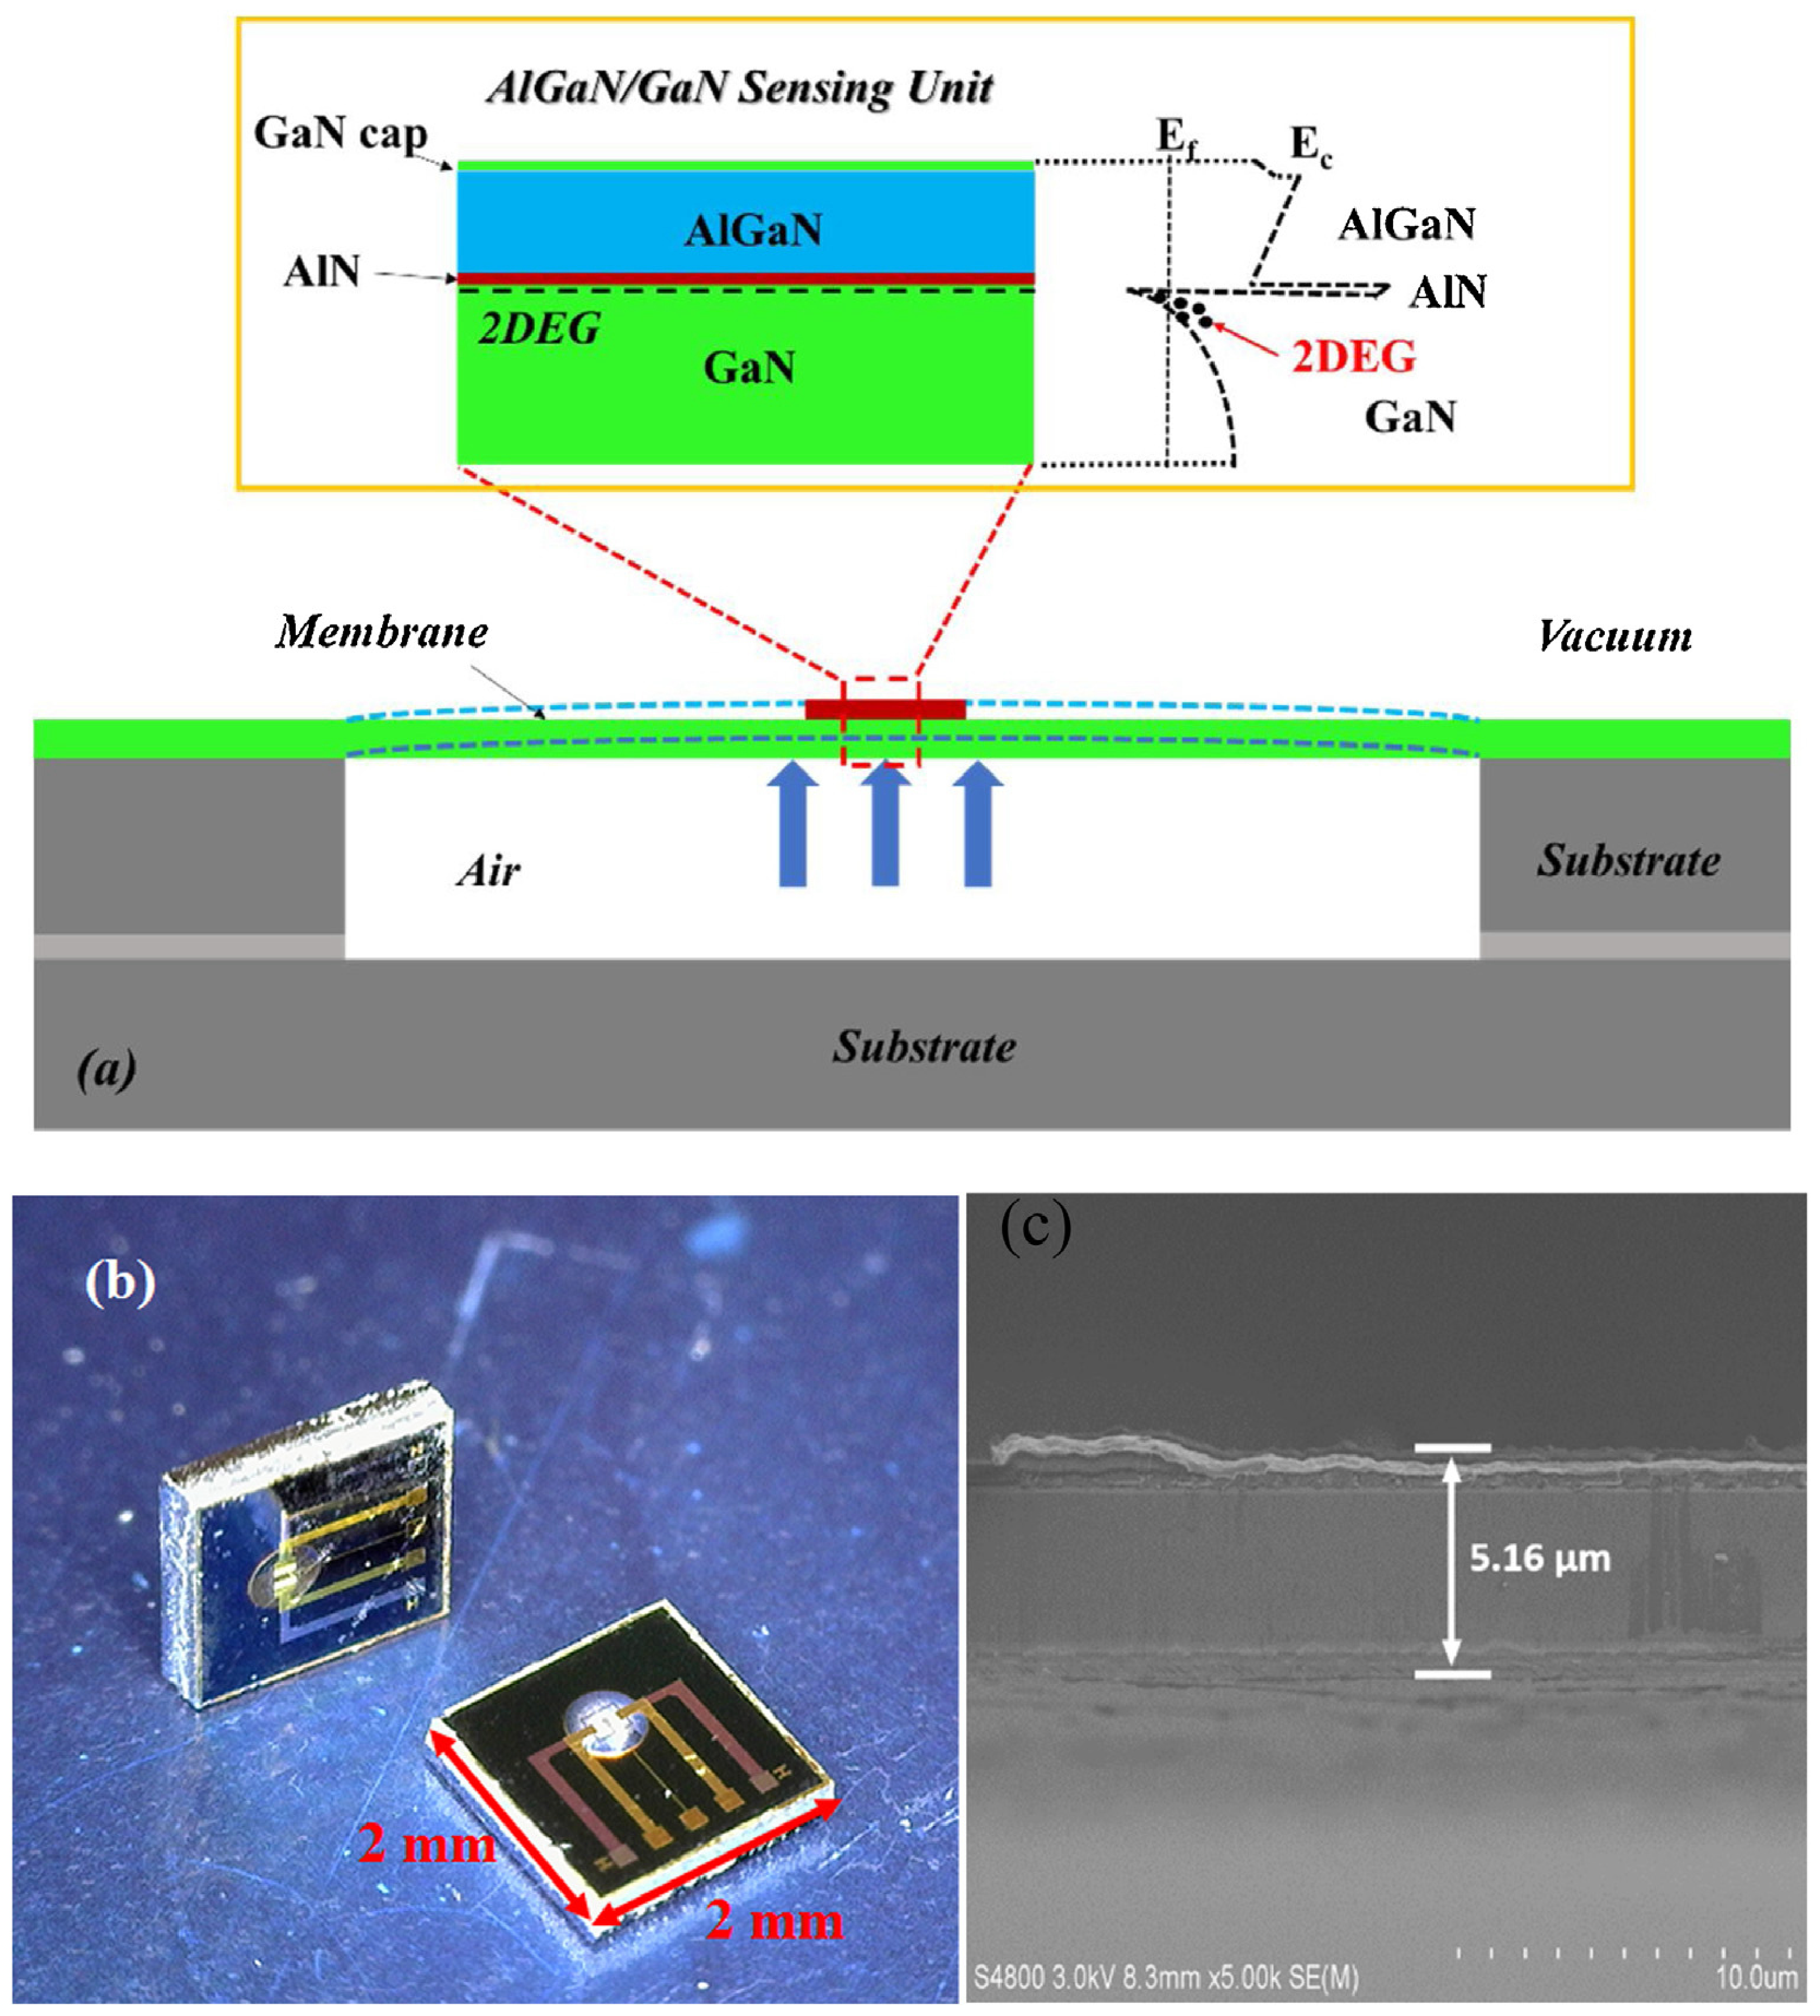
\includegraphics[width=0.9\textwidth]{ch1_16}
\caption[Miniature pressure MEMS sensor based on AlGaN/GaN heterojunction suspended structure]{Miniature pressure MEMS sensor based on AlGaN/GaN heterojunction suspended structure \protect\cite{sun2020low}}
\label{fig:1.16}
\end{figure}


III-V nitride \index{Nitride} MEMS \index{MEMS} devices are also widely used in the field of biosensing. Indu Sarangadharan et al. reported a highly sensitive AlGaN/GaN \index{HEMT} HEMT bioMEMS sensor for detecting cardiac troponin I (\autoref{fig:1.17}) \cite{sarangadharan2018high}. The unique double-layer gate-controlling mechanism overcomes the shortcomings of charge screening in conventional Si-based MEMS biosensors and enables detection of target proteins in physiological solutions without sample processing 


\begin{figure}[H] 
\centering    
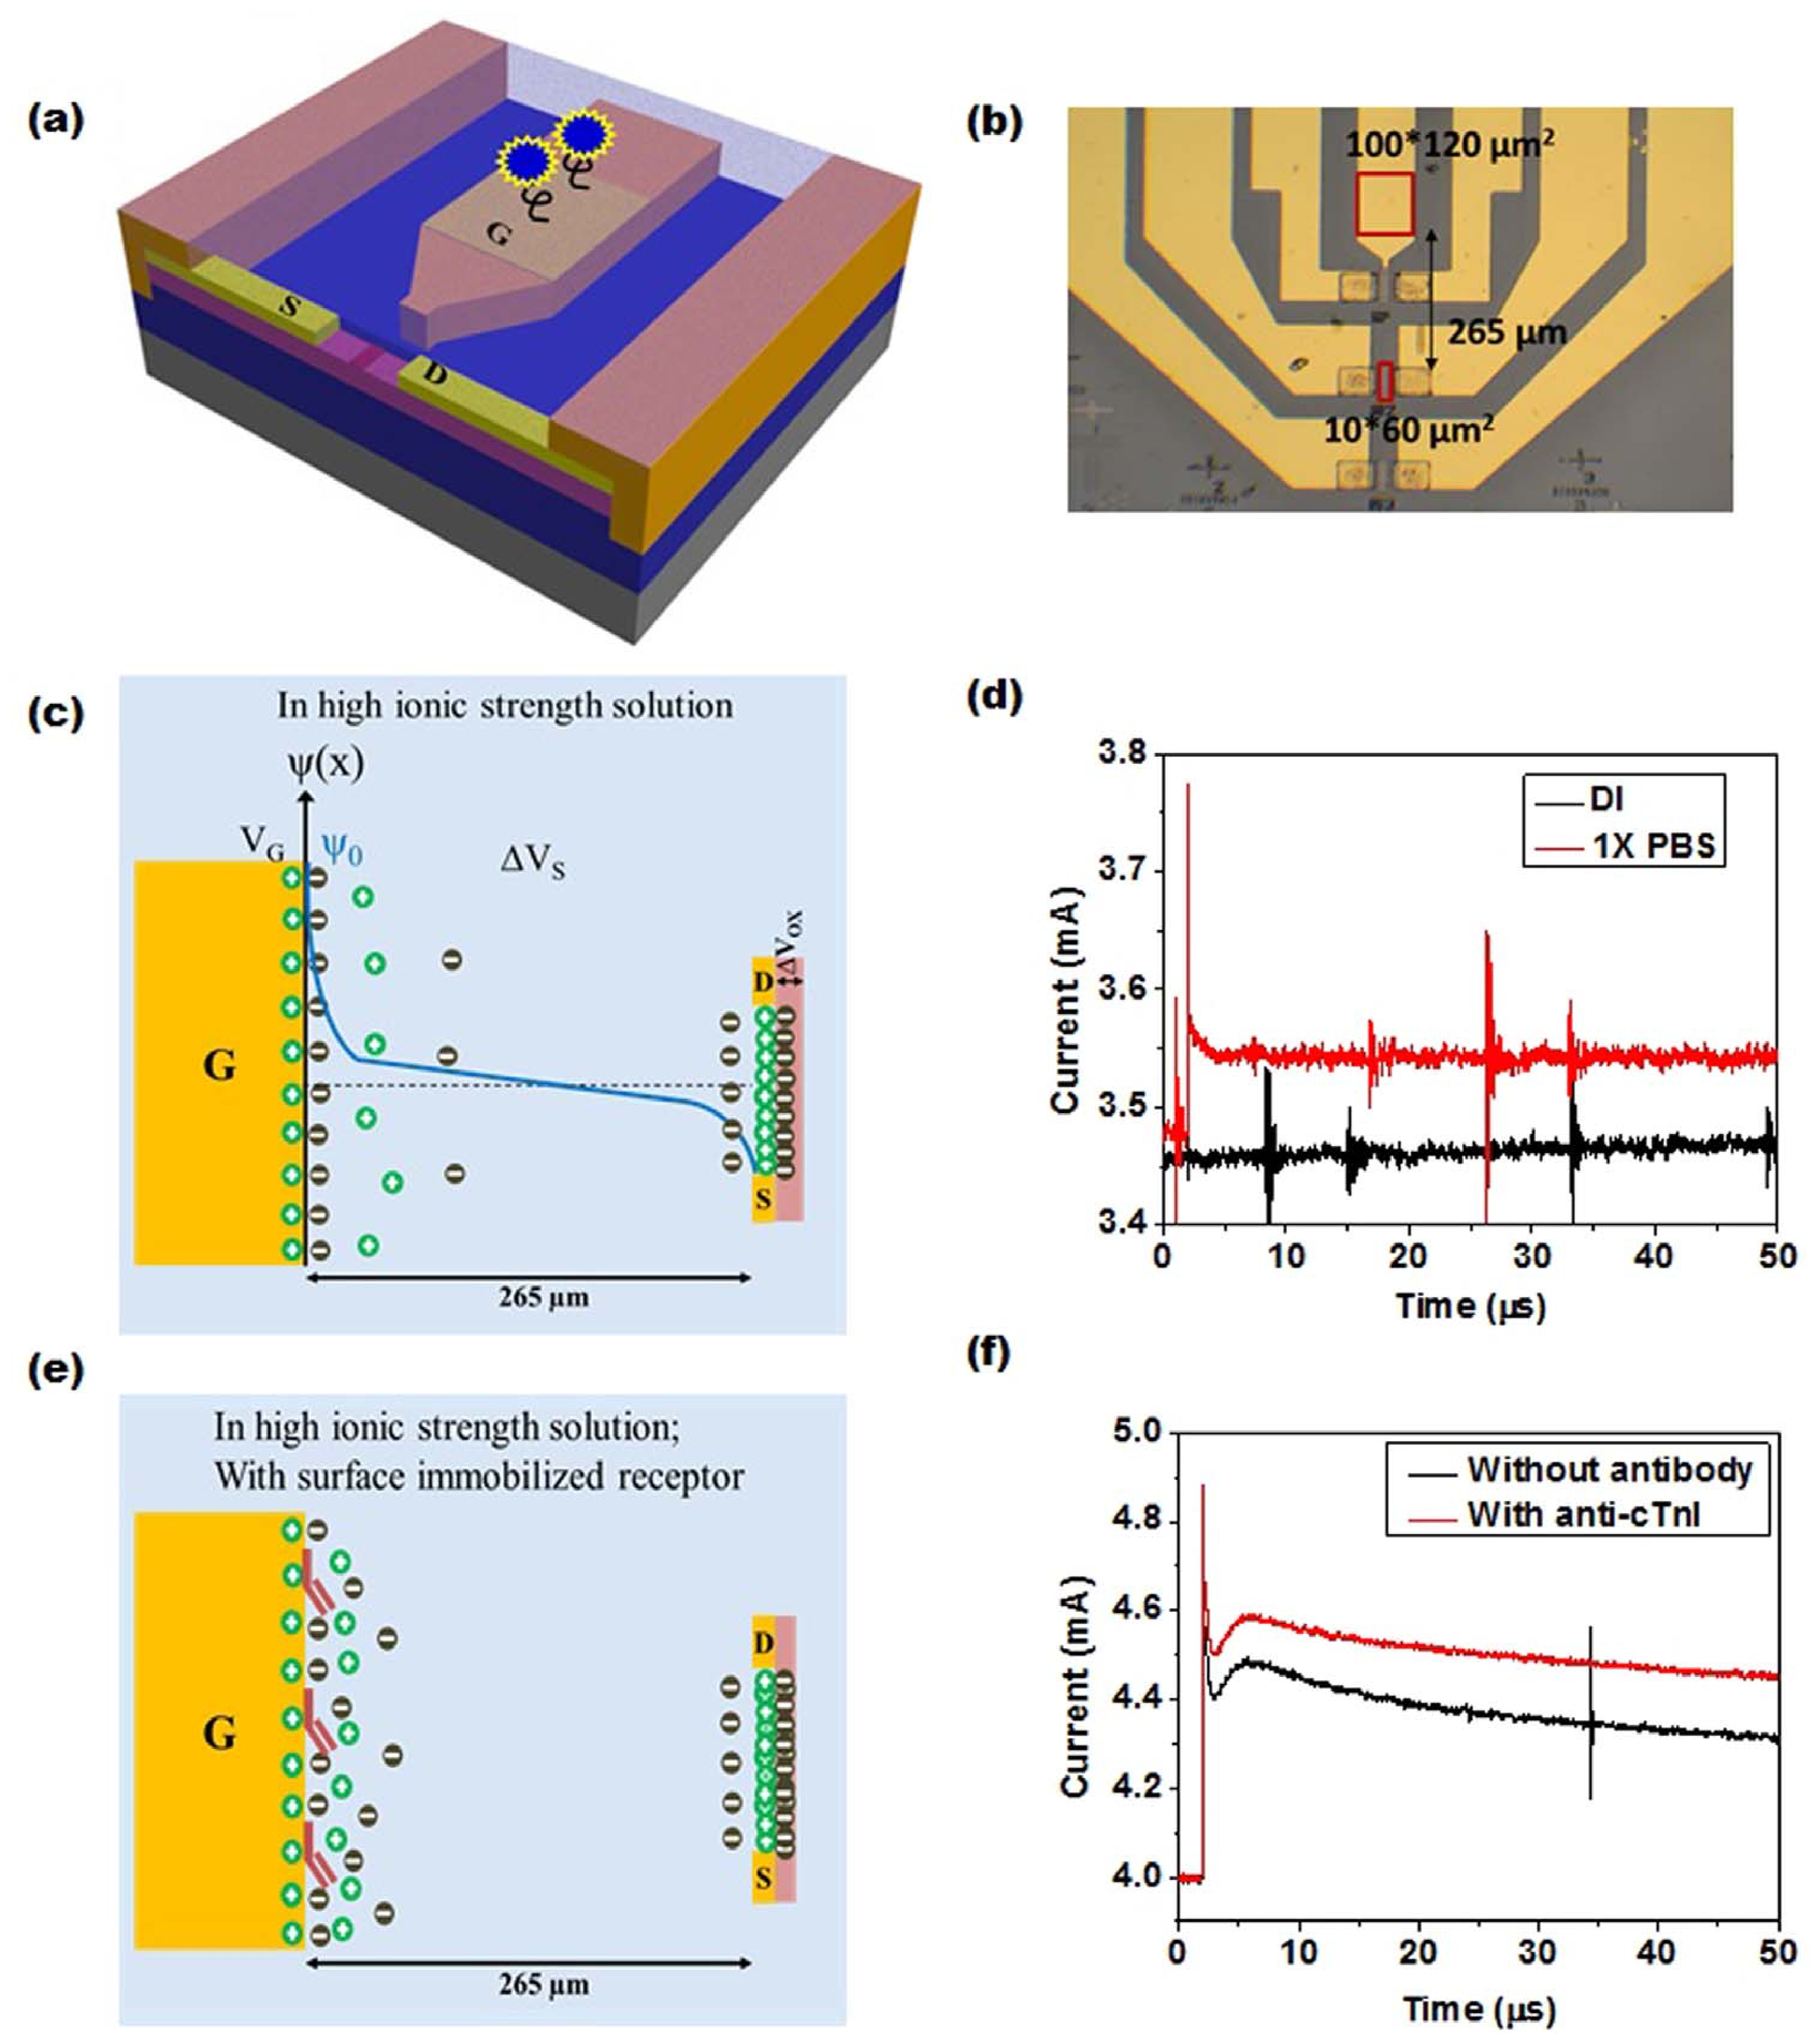
\includegraphics[width=0.9\textwidth]{ch1_17}
\caption[AlGaN/GaN HEMT MEMS biosensor for detecting cardiac troponin I in a physiological environment]{AlGaN/GaN HEMT MEMS biosensor for detecting cardiac troponin I in a physiological environment \protect\cite{sarangadharan2018high}}
\label{fig:1.17}
\end{figure}

\noindent steps, thus greatly simplifying the biosensor system. Tests using purified protein solutions and clinical serum samples showed that the sensor has high sensitivity, specificity, and a wide dynamic range (0.006 $\sim$ 148 \unit{ng/mL}) to quantitatively detect Calcin I in serum samples with sample volumes less than 2 \unit{uL} within 5 minutes. In addition, MEMS \index{MEMS} chips can be packaged in polymer substrates for easy integration with portable measurement units, which can serve as a fast, inexpensive, and highly sensitive cardiovascular disease detection device with broad applications in point-of-care diagnostics and personal healthcare systems.

\subsection{Microstructure of III-V nitrides}

With the deepening of the research on the properties of wide-bandgap semiconductor materials, the preparation technology of III-V \index{Nitride} nitrides has made significant progress. More complex MEMS \index{MEMS} devices structures can be prepared by heterojunction epitaxial \index{Epitaxial!growth} growth, thin film \index{Thin film} deposition (epitaxial film and polycrystalline film), inductively coupled plasma (ICP) \index{Inductively coupled plasma (ICP)} etching process, and photoelectrochemical (PEC) etching process \cite{strittmatter2004development,zorman2008micro,brueckner2011micro,yamada2021fabrication,davies2004fabrication,lv2011characterization-a,lv2011characterization-b}.

\begin{figure}[H] 
\centering    
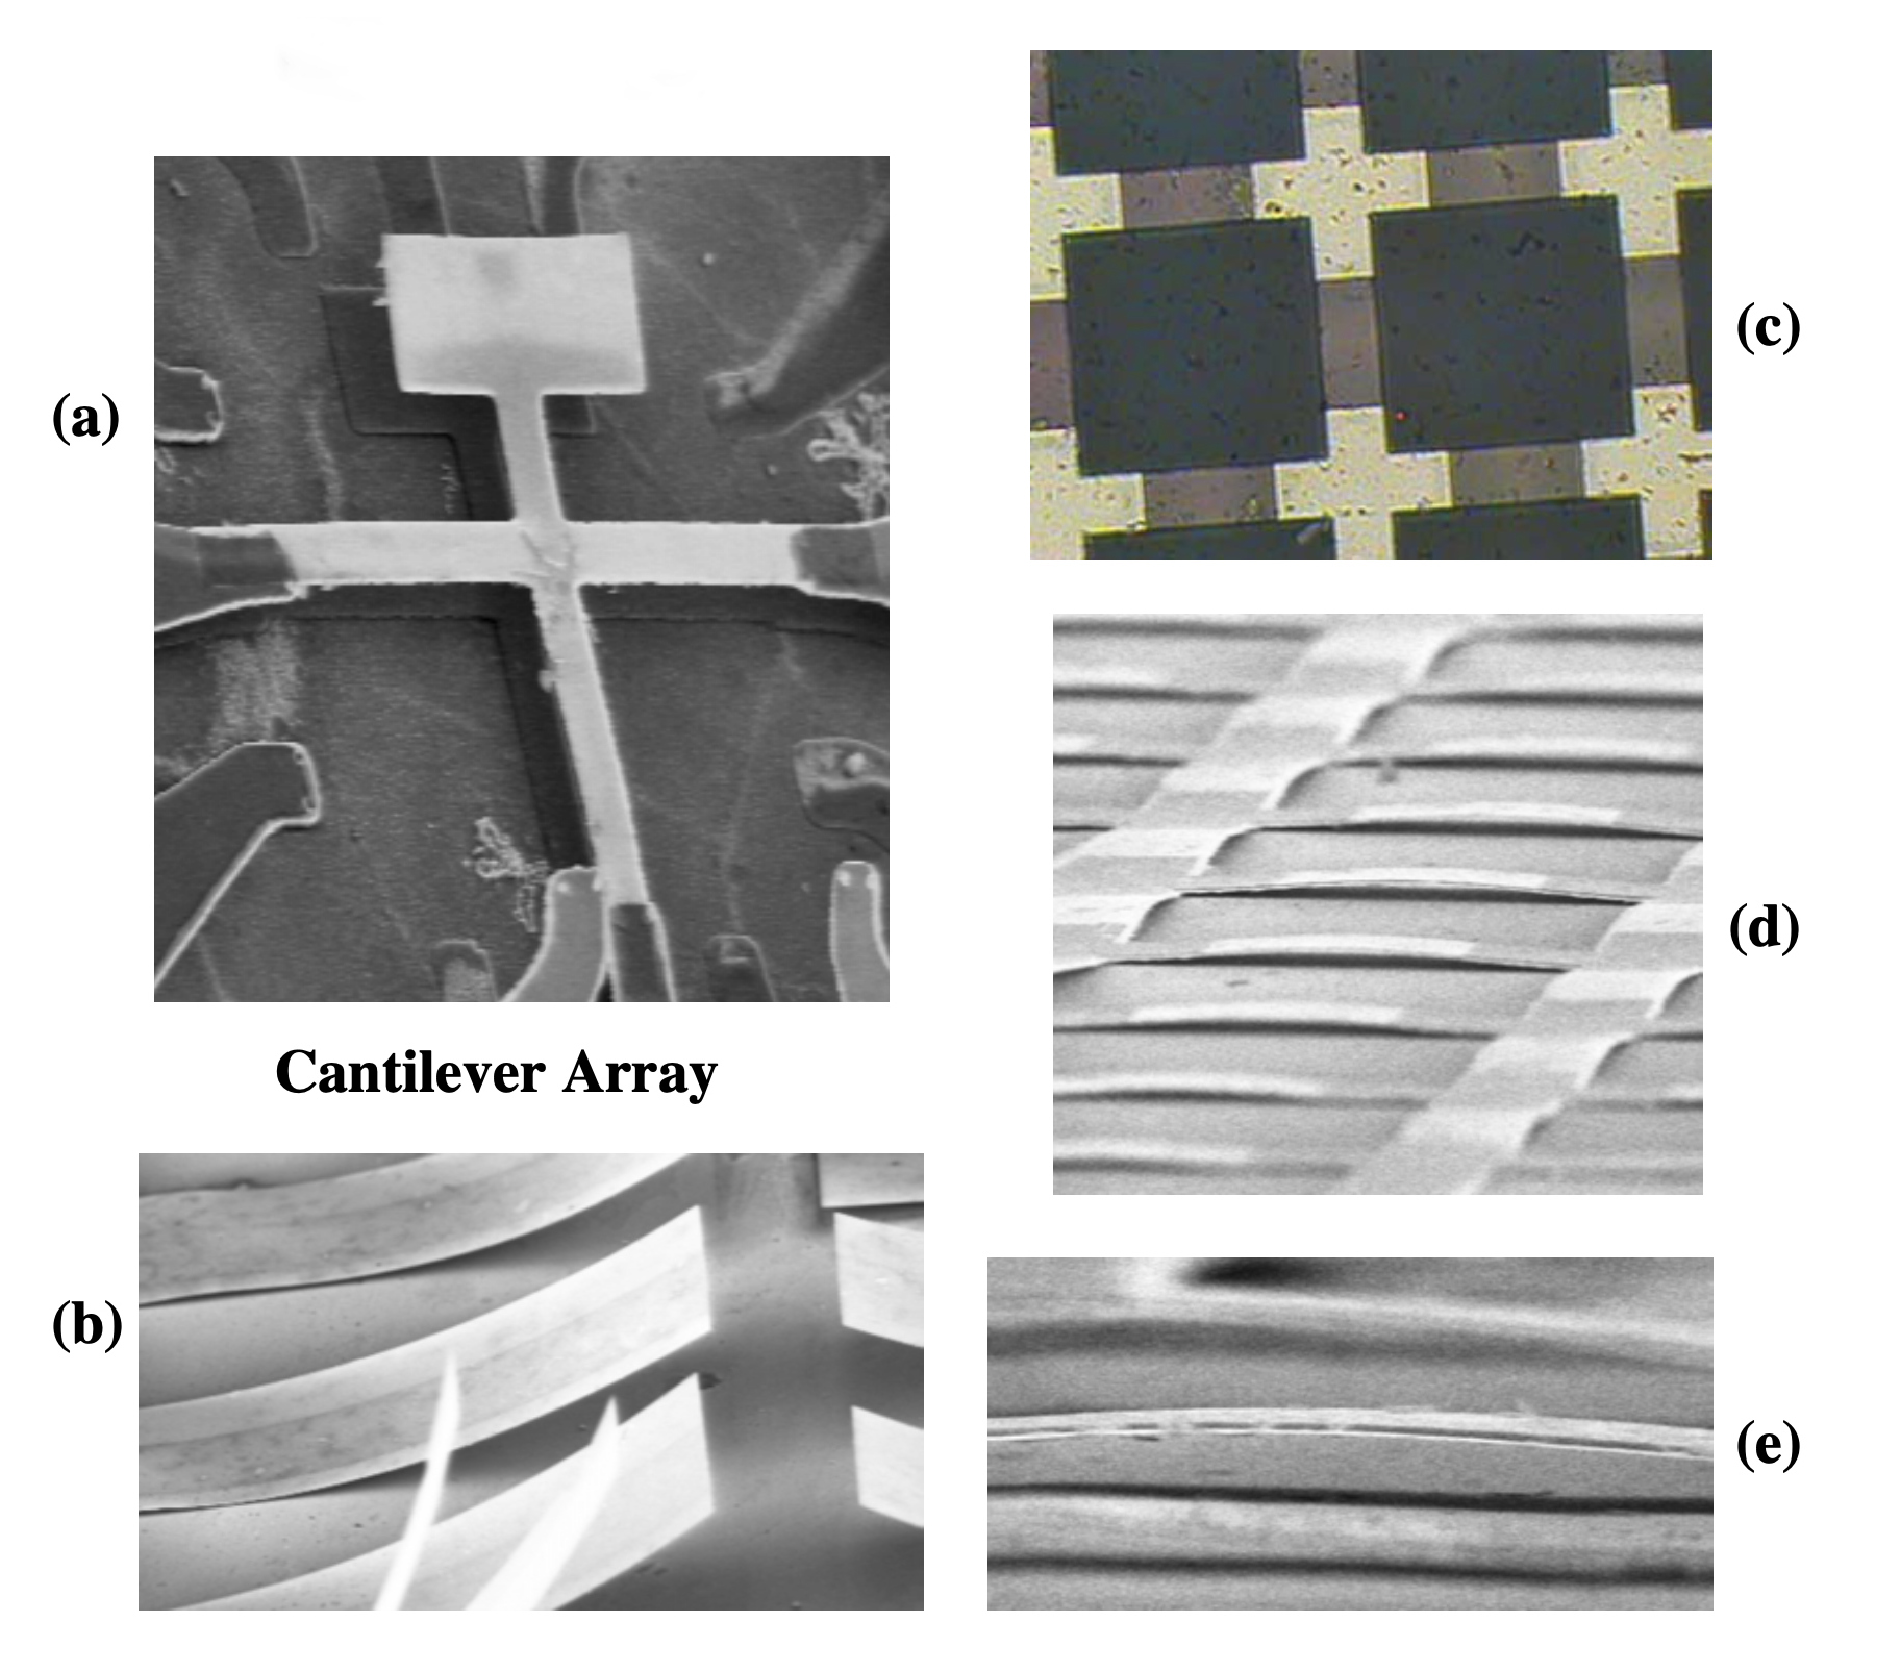
\includegraphics[width=0.9\textwidth]{ch1_18}
\caption[SEM image of a series of p-GaN microcantilever arrays]{SEM image of a series of p-GaN microcantilever arrays \protect\cite{strittmatter2004development}}
\label{fig:1.18}
\end{figure}

\begin{figure}[H] 
\centering    
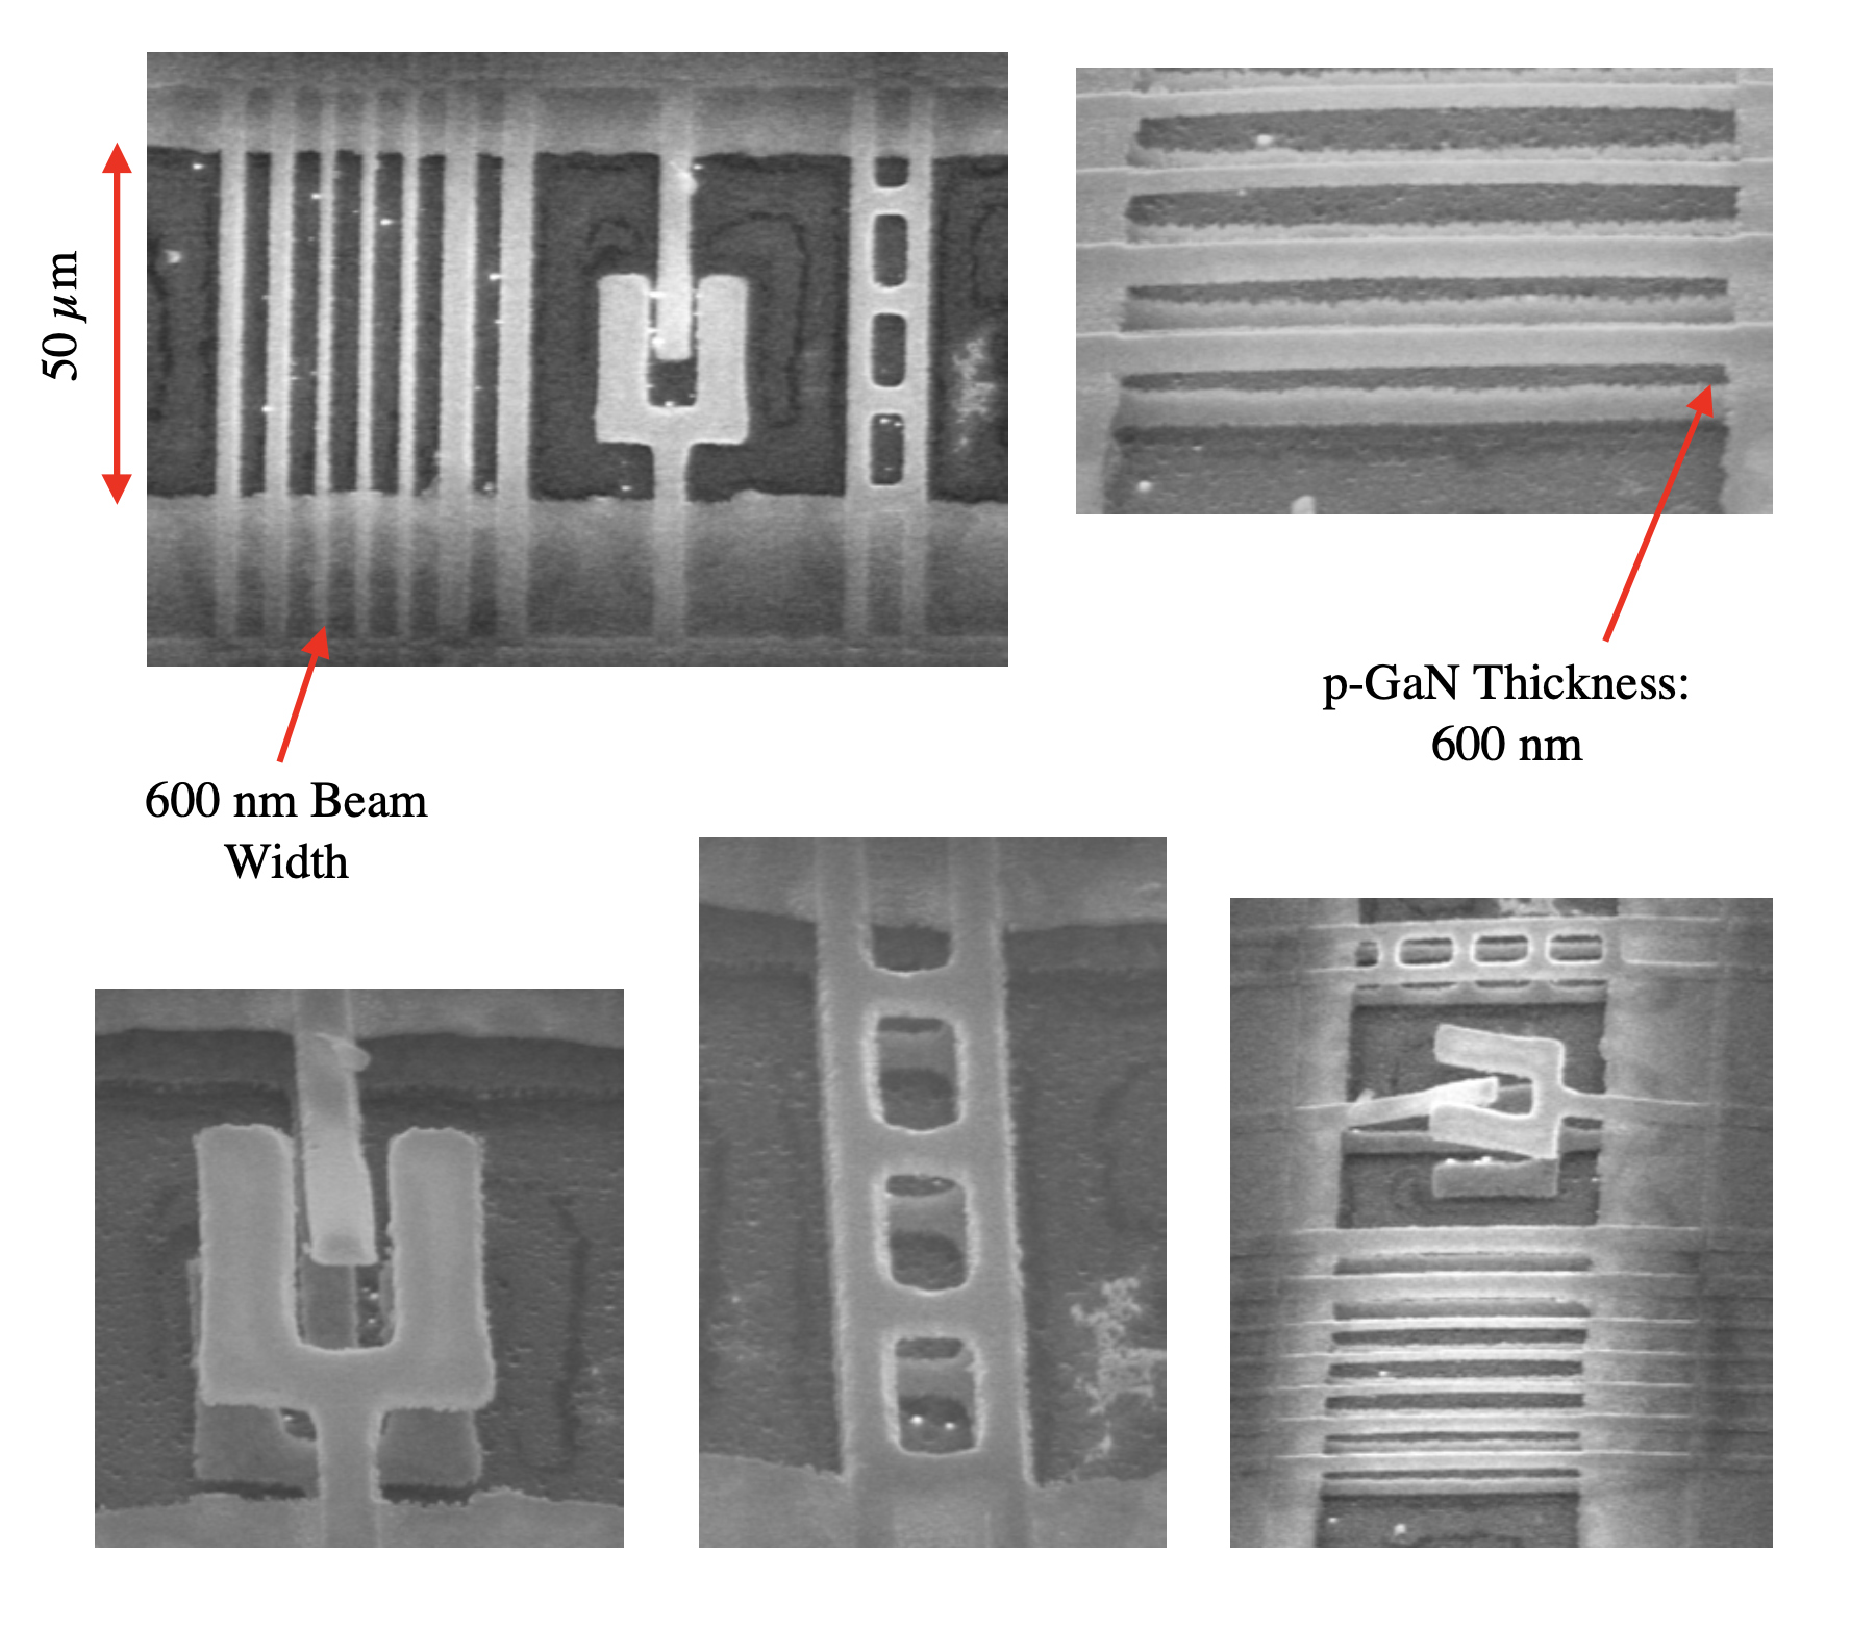
\includegraphics[width=0.9\textwidth]{ch1_19}
\caption[SEM image of a series of p-GaN structures suspended between two half-plane supports]{SEM image of a series of p-GaN structures suspended between two half-plane supports \protect\cite{strittmatter2004development}}
\label{fig:1.19}
\end{figure}

\autoref{fig:1.18} shows a series of p-GaN microcantilever arrays fabricated by a PEC etch process. The etched p-GaN cantilever \index{Cantilever} relaxes into a uniformly curved shape along the direction away from the \index{Substrate} substrate. This is because a vertical stress gradient is introduced in the p-GaN layer due to crystal \index{Crystal} defects during the growth process \cite{strittmatter2004development}. \autoref{fig:1.19} shows a series of p-GaN structures suspended between two half-support planes fabricated by the PEC process, with a lateral dimension of about 1 \unit{\um} and a minimum beam width of only 600 \unit{\nm}. The lateral dimension of the device reaches the sub-micron scale, which indicates that GaN-based MEMS devices can be easily extended to the field of nano-electromechanical systems (NEMS). Advances in III-V nitride \index{Nitride} preparation technology have greatly promoted the development of new III-V nitride power MEMS \index{MEMS} devices.

\section{Outline of the thesis} 

\noindent This thesis systematically studies the theoretical modeling and device fabrication of III-V nitride power MEMS based on the cantilever \index{Cantilever} structure of \index{AlGaN/AlN/GaN heterojunction} AlGaN/AlN/GaN heterojunction. \autoref{fig:1.20} illustrates the structure and SEM \index{Scanning electron microscopy (SEM)} image of GaN power MEMS devices. The active area \index{Active region} is at the junction of the cantilever and the \index{Wafer} wafer, which is enlarged in the figure. Due to the design of cantilever \index{Cantilever} structure, the external stimulus from direct \index{Strain} strains or non-contact magnetic force \index{Magnetic!force} will be greatly amplified, thereby introducing the piezoelectric polarization charges \index{Piezoelectric!polarization charge} in the active \index{Active region} area. Based on the piezotronics \index{Piezotronics} effect, the piezoelectric polarization charges generated by external stimulus can modulate the energy band at the AlGaN/AlN/GaN heterojunction, thereby effectively adjusting the 2DEG concentration \index{Two-dimensional electron gas (2DEG)} and finally controlling the output current \index{Output!current} and power density of the MEMS devices.

\begin{figure}[H] 
\centering    
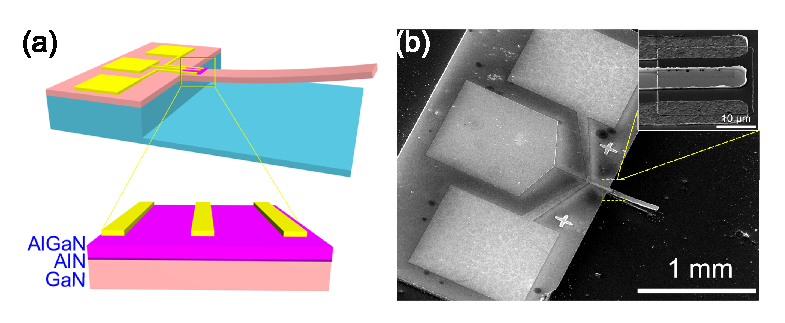
\includegraphics[width=0.9\textwidth]{ch1_20}
\caption[Structure and SEM image of GaN power MEMS devices]{Structure and SEM image of GaN power MEMS devices}
\label{fig:1.20}
\end{figure}

The physical framework \index{Physical!framework} and mathematical analysis method are presented to model the modulation \index{Modulation} characteristics of the external stress on the energy band \index{Energy band} of the \index{AlGaN/AlN/GaN heterojunction} AlGaN/AlN/GaN heterojunction and the electrical properties of the MEMS \index{MEMS} device, which provide theoretical guidance for the design of III-V nitride \index{Nitride} power MEMS. On this basis, two types of novel power MEMS \index{MEMS} devices based on the cantilever \index{Cantilever} structure of \index{AlGaN/AlN/GaN heterojunction} AlGaN/AlN/GaN heterojunctions were designed and fabricated, namely, a strain-controlled power MEMS devices (SPD) \index{Strain-controlled power MEMS devices (SPD)} and a \index{Magnetosensory power MEMS devices (MPD)} magnetic field-controlled power MEMS devices (MPD), in which external strain \index{Strain} and magnetic field \index{Magnetic!field} can significantly modulate \index{Modulation} the output power \index{Output!power} density of MEMS \index{MEMS} devices due to the micro-cantilever \index{Cantilever} structure.\\

\begin{figure}[H] 
\centering    
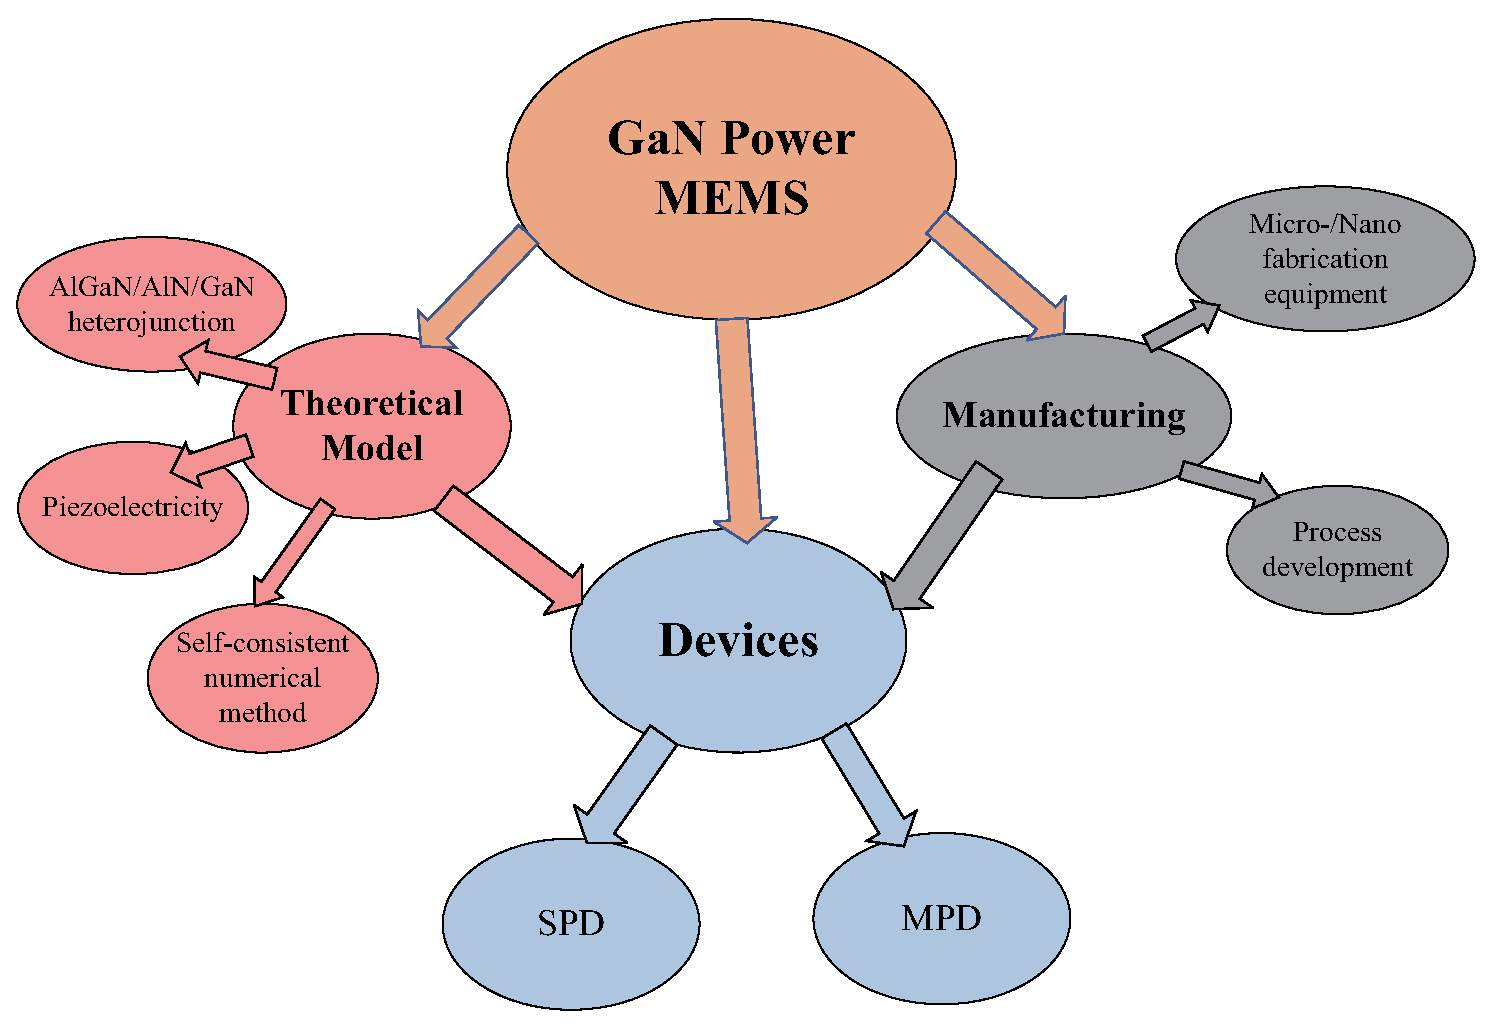
\includegraphics[width=0.9\textwidth]{Outline}
\caption[The outline of the thesis]{The outline of the thesis}
\label{fig:outline}
\end{figure}

\noindent The content of this thesis is mainly composed of the following three parts: \\

\begin{large}
\centerline{Part \uppercase\expandafter{\romannumeral1} \quad Theory}
\end{large}

~\\

\noindent Chapter 2. Theoretical model of MEMS cantilever devices\\

\noindent In this study, a semi-classical physical model of the MEMS \index{MEMS} device with a cantilever \index{Cantilever} structure based on \index{AlGaN/AlN/GaN heterojunction} AlGaN/AlN/GaN heterojunction was established using piezotronics \index{Piezotronics} theory. The mathematical relationship between the lattice strain \index{Lattice!strain} of the thin film \index{Thin film} and the piezoelectric polarization charge intensity \index{Piezoelectric!polarization charge} in the multilayer heterojunction was deduced through piezoelectric constitutive equation \index{Piezoelectric!constitutive equation} and biaxial stress \index{Biaxial stress model} model. The finite element analysis \index{Finite element analysis} method of material mechanics is used to calculate the piezoelectric polarization charge intensity of the heterojunction film under different external stresses, and then the self-consistent coupling computational model \index{Self-consistent computational model} of the one-dimensional Schrödinger-Poisson coupling equation \index{Schrödinger-Poisson coupling equation} was used to calculate the modulation \index{Modulation} characteristics of the external stress on the \index{Two-dimensional electron gas (2DEG)} 2DEG concentration and energy band \index{Energy band} of the AlGaN/AlN/GaN heterojunction, as well as the electrical properties of the MEMS device. Based on the theoretical model, the new AlGaN/AlN/GaN power MEMS have been designed and fabricated, namely \index{Strain-controlled power MEMS devices (SPD)} SPD and \index{Magnetosensory power MEMS devices (MPD)} MPD. This study provides theoretical guidance for the development of new MEMS cantilever \index{Cantilever} devices based on AlGaN/AlN/GaN heterojunctions.\\

\begin{large}
\centerline{Part \uppercase\expandafter{\romannumeral2} \quad Manufacturing}
\end{large}

~\\

\noindent Chapter 3. Manufacturing Technology of Power MEMS Devices\\

\noindent In the Part II, the manufacture of GaN power MEMS devices from epitaxial growth \index{Epitaxial!growth} wafers \index{Wafer} to well-functional devices will be systematically studied. Benefiting from the rapid development of III-V compound semiconductor fabrication and characterization equipment, various complex microstructures including GaN microcantilever \index{Cantilever} structures can now be easily realized by equipment with different functions. This chapter introduced the main nanofabrication and characterization equipment, including epitaxial \index{Epitaxial!growth} growth, dry \index{Etching!dry etching} etching, photolithograph\index{Photolithography}y, thin film \index{Thin film} deposition, plasma \index{Cleaning!plasma cleaning} cleaning, Raman \index{Raman!spectroscopy} spectroscopy, scanning \index{Scanning electron microscopy (SEM)} electron microscopy, transmission \index{Transmission electron microscopy (TEM)} electron microscopy, etc. I briefly introduced their important role in GaN power MEMS \index{MEMS} research, as well as the corresponding process \index{Fabrication process} design and key parameters.\\

\noindent Chapter 4. Process Development and Integration of Power MEMS Devices\\

\noindent In this chapter, I developed the corresponding process parameters and their process integration based on the manufacturing technology and equipment, thus realizing the whole process from GaN wafer \index{Wafer} to device. The processes in this chapter have been described in detail about the main purpose of the process, the equipment used, and the detailed recipe parameters. Moreover, in order to visualize the fabrication \index{Fabrication process} process flow, a corresponding flow chart has been drawn to illustrate the main process steps. Step by step, high-performance GaN \index{HEMT} HEMTs and GaN power \index{MEMS} MEMS devices have been successfully fabricated.\\

\begin{large}
\centerline{Part \uppercase\expandafter{\romannumeral3} \quad Devices}
\end{large}

~\\

\noindent Chapter 5. Strain-controlled power MEMS devices\\

\noindent In this study, we designed a strain \index{Strain} modulated \index{Modulation} power MEMS device \index{Strain-controlled power MEMS devices (SPD)} (Strain-controlled Power Device, SPD) based on the cantilever structure \index{Cantilever} of \index{AlGaN/AlN/GaN heterojunction} AlGaN/AlN/GaN heterojunction, which uses external strain \index{Strain} to directly modulate \index{Modulation} the output power \index{Output!power} of the device by simulating the reflection process of the human reflex. Based on the piezotronics \index{Piezotronics} effect, the piezoelectric polarization charges \index{Piezoelectric!polarization charge} generated by external strain can modulate the energy band \index{Energy band} at the AlGaN/AlN/GaN heterojunction, thereby effectively adjusting the \index{Two-dimensional electron gas (2DEG)} 2DEG concentration, and finally controlling the output current \index{Output!current} and power density of the SPD. At the same time, similar to the ultimate control ability of the brain in the knee-jerk reflex mechanism, the gate voltage \index{Voltage!gate voltage} of the SPD \index{Strain-controlled power MEMS devices (SPD)} can control the output power \index{Output!power} in a wider range, thus combining the dimensional control advantage of both small-scale external strain \index{Strain} control and large-scale programmable gate voltage \index{Voltage!gate voltage} control, which means that the strain \index{Strain} modulation \index{Modulation} power is programmable. This study not only provides new insights into the interplay of mechanical stimulation and power control, but could also lead to the development of biomimetic smart powered devices that resemble human reflexes.\\

\noindent Chapter 6. Magnetosensory power MEMS devices.\\

\noindent In this study, we fabricated a \index{Magnetic!field} magnetic field-regulated power MEMS device (Magnetosensory Power Devices, MPD) \index{Magnetosensory power MEMS devices (MPD)} by depositing a magnetic thin film \index{Magnetic!thin film} on the front end of a cantilevered \index{Cantilever} GaN HEMT \index{HEMT} based on \index{AlGaN/AlN/GaN heterojunction} AlGaN/AlN/GaN heterojunction, which can directly control the output power \index{Output!power} through an external magnetic field. Moreover, the output power of the MPD has a linear relationship with the external magnetic field, showing good magnetic regulation characteristics. Based on the piezotronics \index{Piezotronics} effect, the magnetic force \index{Magnetic!force} generated by the external magnetic field can generate corresponding piezoelectric polarization charges \index{Piezoelectric!polarization charge} at the interface \index{Interface} of the \index{Thin film} thin film, which can modulate \index{Modulation} the energy band \index{Energy band} of the AlGaN/AlN/GaN heterojunction, thereby effectively adjusting the 2DEG \index{Two-dimensional electron gas (2DEG)} concentration, and finally controlling the output power \index{Output!power} of the MPD. At the same time, similar to the bio-voltage signal between neuron synapses which effectively regulated the magnitude of neuronal signal in a larger range, the output power is controlled at a larger range by the gate voltage \index{Voltage!gate voltage} of MPD. Therefore it combines the two-dimensional control advantage. This work not only provides physical electronics insights into the working mechanism of magnetic sensing neurons in the biological sense, but also can promote the development of various neuroelectronic devices.\\

\part{Theory}

% **************************** Define Graphics Path **************************



%!TEX root = ../thesis.tex
%*******************************************************************************
%****************************** Second Chapter *********************************
%*******************************************************************************

\chapter{Theoretical Model of Power MEMS Devices}
\label{ch:Theoretical Models of MEMS Cantilever Devices based on AlGaN/AlN/GaN Heterostructure}

\ifpdf
    \graphicspath{{Chapter2/Figs/Raster/}{Chapter2/Figs/PDF/}{Chapter2/Figs/}}
\else
    \graphicspath{{Chapter2/Figs/Vector/}{Chapter2/Figs/}}
\fi


% Uncomment this line, when you have siunitx package loaded.
%The SI Units for dynamic viscosity is \si{\newton\second\per\metre\squared}.

\section{Polarization effects of III-V nitrides}
\label{sec:Polarization effect of III-V nitrides}

III-V nitride \index{Nitride} semiconductor materials usually exhibit very obvious polarization \index{Polarization!effect} effects, namely piezoelectric polarization \index{Piezoelectric!polarization} and \index{Spontaneous polarization} spontaneous polarization. Due to the lack of inversion symmetry centers in semiconducting nitrides, a prominent piezoelectric polarization effect is exhibited when the lattice is strained \index{Strain} along <0001>. The piezoelectric coefficient \index{Piezoelectric!coefficient} in nitrides is almost an order of magnitude larger than many conventional III-V semiconductors \cite{bykhovski1993influence,bykhovski1997elastic,gualtieri1994piezoelectric,o1973acoustic}. The piezoelectric polarization effect has two components, one is lattice strain \index{Lattice!strain} caused by lattice mismatch \index{Lattice!mismatch} between the substrate \index{Substrate} and the epitaxial layer \index{Epitaxial!layer} and the other is thermal strain caused by the difference in thermal expansion coefficient between the substrate \index{Substrate} and the \index{Epitaxial!layer} epitaxial layer. Furthermore, due to the low symmetry of nitrides, there is a spontaneous polarization \index{Spontaneous polarization} effect in ideal \index{Wurtzite} wurtzite-structured nitrides, which induces intrinsic spontaneously polarized charges at the material \index{Surface} surface \cite{resta1994macroscopic,king1993theory}. Especially when involving the heterojunction interface \index{Interface} between two nitride semiconductors with different \index{Electronegativity} electronegativities, the spontaneous polarization charge at the heterojunction interface caused by the spontaneous polarization effect can significantly modulate the heterojunction energy band \index{Energy band} and optoelectronic properties.

Due to polarization effects in III-V nitride \index{Nitride} semiconductor materials, there is a high density of polarization charges \index{Polarization!charge} at the interface \index{Interface} of heterojunction devices with significant lattice strain \index{Lattice!strain} (such as HEMTs), and polarization charges \index{Polarization!charge} are closely related to the energy \index{Energy band} band, free carrier distribution \index{Carrier!distribution} and density in the heterojunction. Therefore, polarization effects \index{Polarization!effect} affect the performance of all nitride-based semiconductor devices, especially \index{HEMT} HEMTs. Unless using non-polar surfaces \index{Surface} (such as a-planes), material polarization effects must be considered in device design. Taking the AlGaN/AlN/GaN \index{AlGaN/AlN/GaN heterojunction} heterojunction as an example, as mentioned above, in the absence of external \index{Strain} strain, the polarization charge at the interface \index{Interface} of the heterojunction has two origins: the piezoelectric polarization \index{Piezoelectric!polarization charge} charge ($P_{PE}$) caused by lattice mismatch \index{Lattice!mismatch} between films, and the spontaneous polarization \index{Spontaneous polarization} charge ($P_{SP}$) of the film itself. Generally the spontaneous polarization in the AlGaN/AlN/GaN heterojunction is larger than the piezoelectric polarization in the absence of external strain, and the strain in the heterojunction film decreases when defect-related relaxation occurs, resulting in a weakening of the \index{Piezoelectric!polarization} piezoelectric polarization. These polarized charges are present to varying degrees in all III-V nitride \index{Nitride} semiconductors unless counteracted by considering lattice symmetry in a particular direction (eg, non-polar surfaces). Since the spontaneous polarization and piezoelectric polarization charges in III-V nitride semiconductor materials can significantly affect the energy band \index{Energy band} of the heterojunction, thereby changing the optoelectronic properties of the heterojunction, the electrical performance of AlGaN/AlN/GaN \index{AlGaN/AlN/GaN heterojunction} MEMS \index{MEMS} can be effectively modulated by artificially changing the piezoelectric polarization charge in the material \cite{kim2013polarization,jena2011polarization,verma2018polarization}.

The polarization effect \index{Polarization!effect} depends on the polarity of the \index{Crystal} crystal. For GaN crystals, the $[0001]$ oriented crystals are called Ga polar crystals, and the $[000\overline{1}]$ oriented crystals are called N polar crystals. It is worth noting that polarity is a bulk property of a material, not a surface \index{Surface} property. One can imagine a situation in which N-polar GaN is covered by a monolayer of Ga, but the orientation and polarity of the crystal \index{Crystal} remain unchanged. Therefore, the polarity of GaN can usually be judged by the following way. When the bond (single bond) along the c-direction of the crystal is from $Ga^{+}$ ion to $N^{-}$ ion, the polarity is called Ga polarity. Similarly, when the bonds (single bonds) in the c-direction of the crystal are from $N^{-}$ ions to $Ga^{+}$ ions, the polarity is called N-polarity. Briefly, Ga-polar crystals mean that if the crystal is cut along the c-plane, but only a single bond of the tetrahedral lattice is broken, the surface of the final crystal is a Ga-plane. The opposite is true for N-polar crystals. Studies have shown that the polarity faces of III-V nitride \index{Nitride} semiconductor materials have a significant impact on heterojunction energy band \cite{jang2002characterization}, 2DEG concentration \cite{dimitrov2000two}, electrical properties \cite{guerra2010comparison,dimitrov1999comparison}, short channel effect \cite{park2011simulation}, and light reflection \cite{buchheim2004photoreflectance}, and other optoelectronic properties.

\begin{figure}[H] 
\centering    
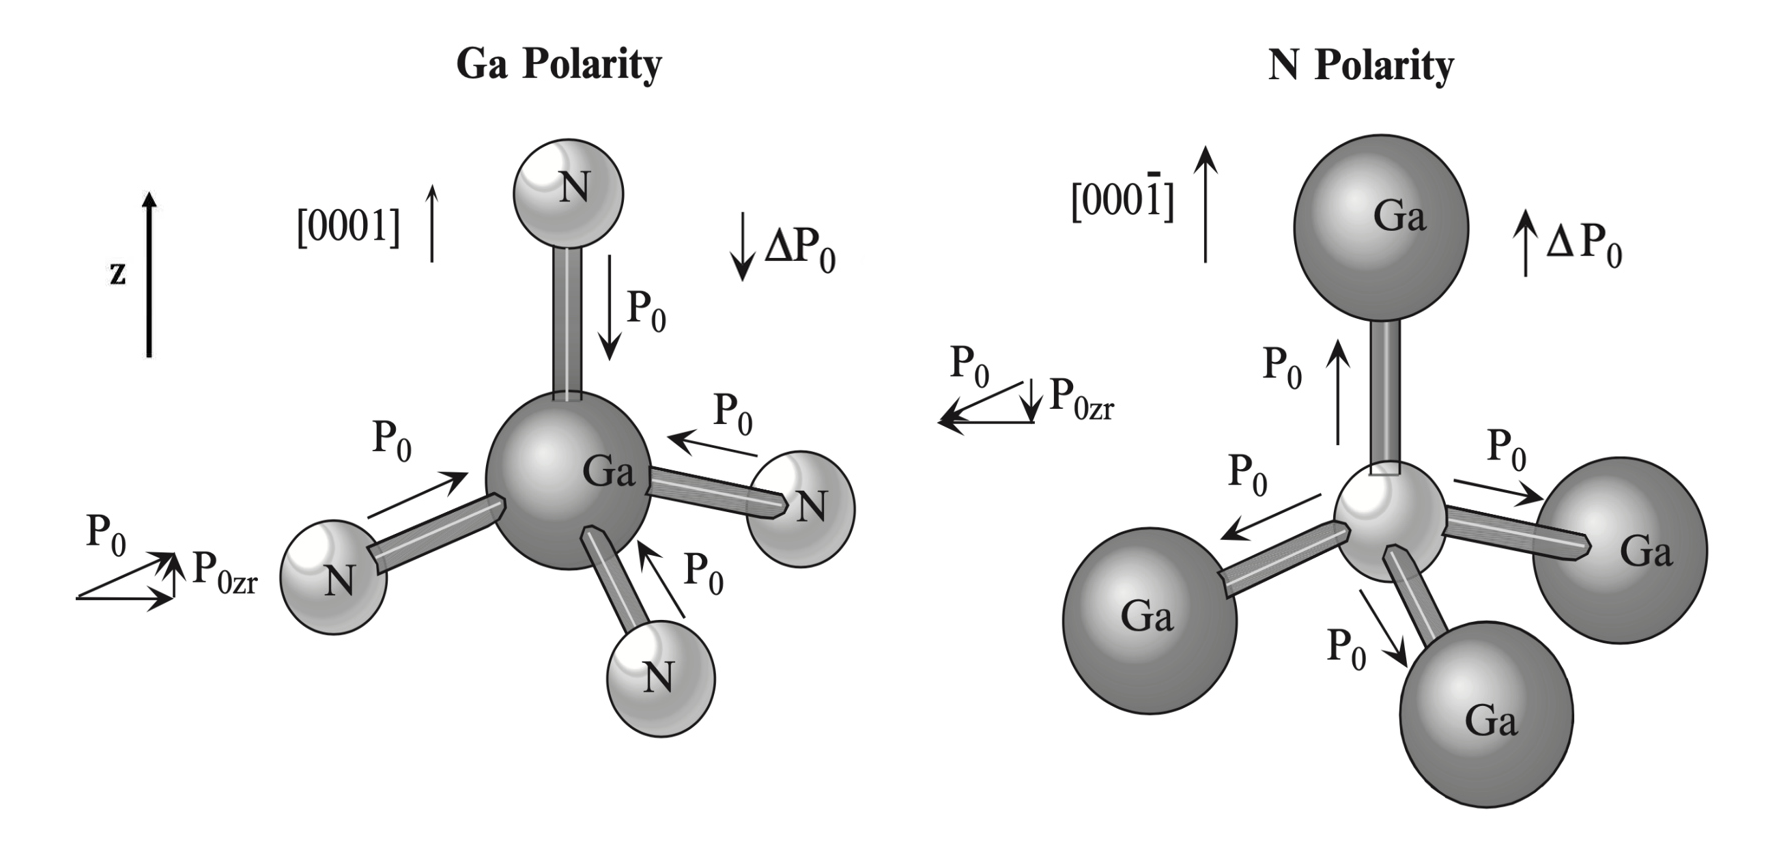
\includegraphics[width=0.9\textwidth]{ch2_1}
\caption[Ball and stick model of an ideal GaN crystal with Ga and N-polarity in a relaxed state]{Ball and stick model of an ideal GaN crystal with Ga and N-polarity in a relaxed state \protect\cite{morkoc2008polarization}}
\label{fig:2.1}
\end{figure}

The effects of polarization due to the low symmetry of the lattice (spontaneous \index{Spontaneous polarization} polarization) and the lattice strain \index{Lattice!strain} of the heterojunction interface \index{Interface} (piezoelectric \index{Piezoelectric!polarization} polarization) can be visualized by the simplified ball and stick model. Shown in \autoref{fig:2.1} is a ball-and-stick diagram of the tetrahedral lattice between $Ga$ ions and $N$ ions in the relaxed Ga-polar and N-polar 

\begin{figure}[H] 
\centering    
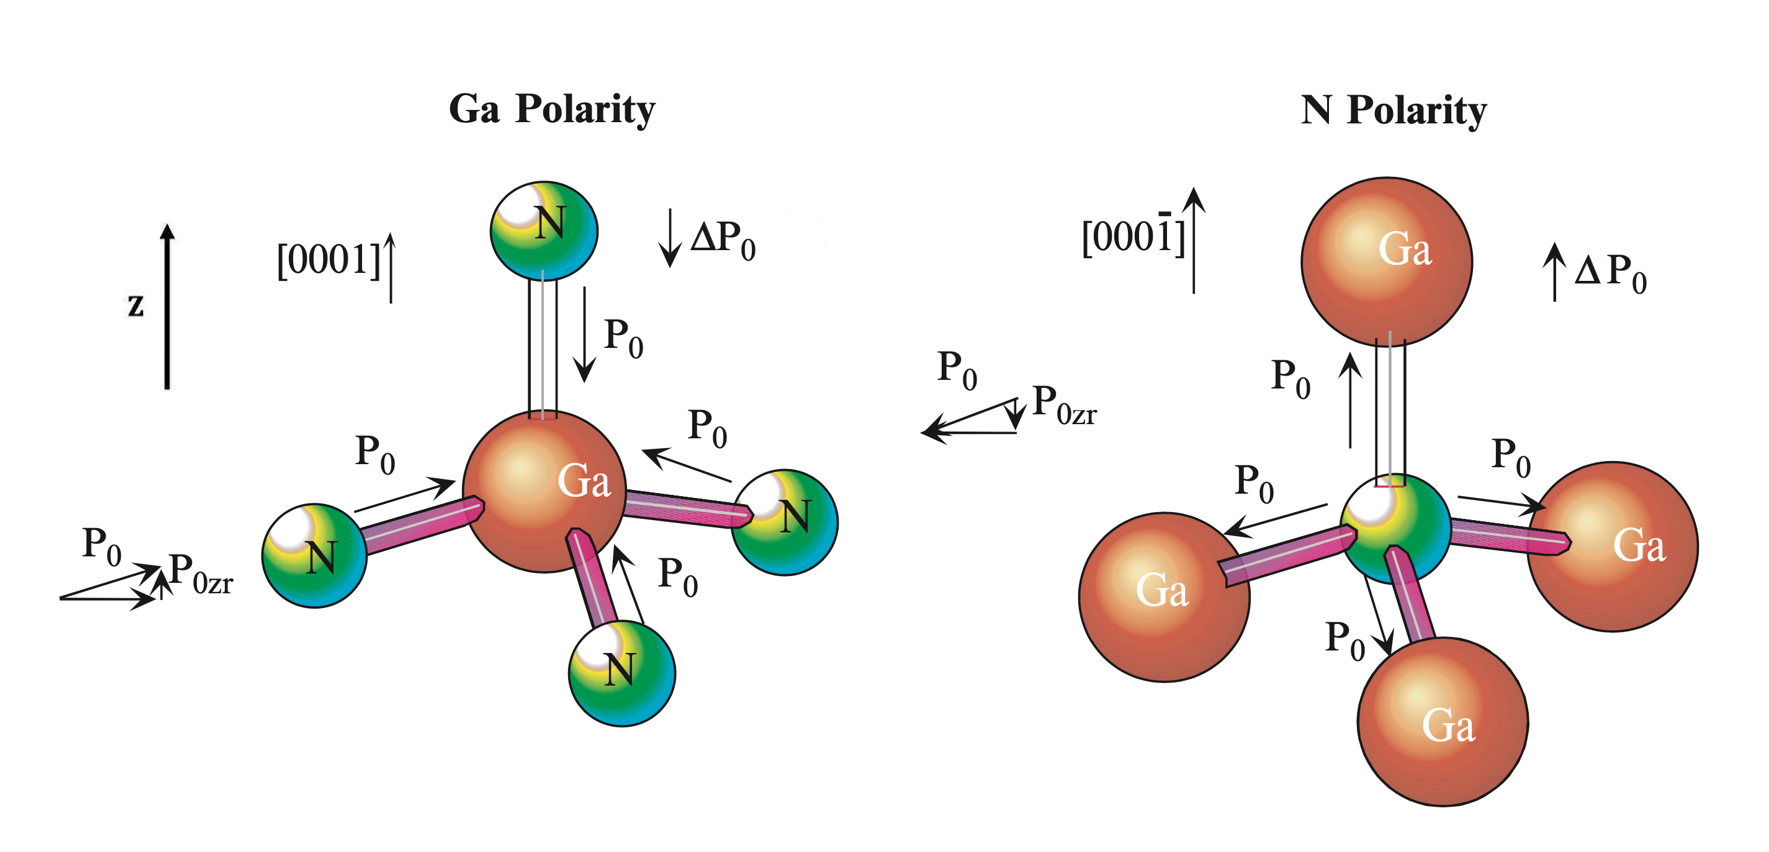
\includegraphics[width=0.9\textwidth]{ch2_2}
\caption[Ball and stick model of a GaN crystal for both Ga and N polarity with a homogeneous in-plane tensile strain]{Ball and stick model of a GaN crystal for both Ga and N polarity with a homogeneous in-plane tensile strain \protect\cite{morkoc2008polarization}}
\label{fig:2.2}
\end{figure}

\begin{figure}[H] 
\centering    
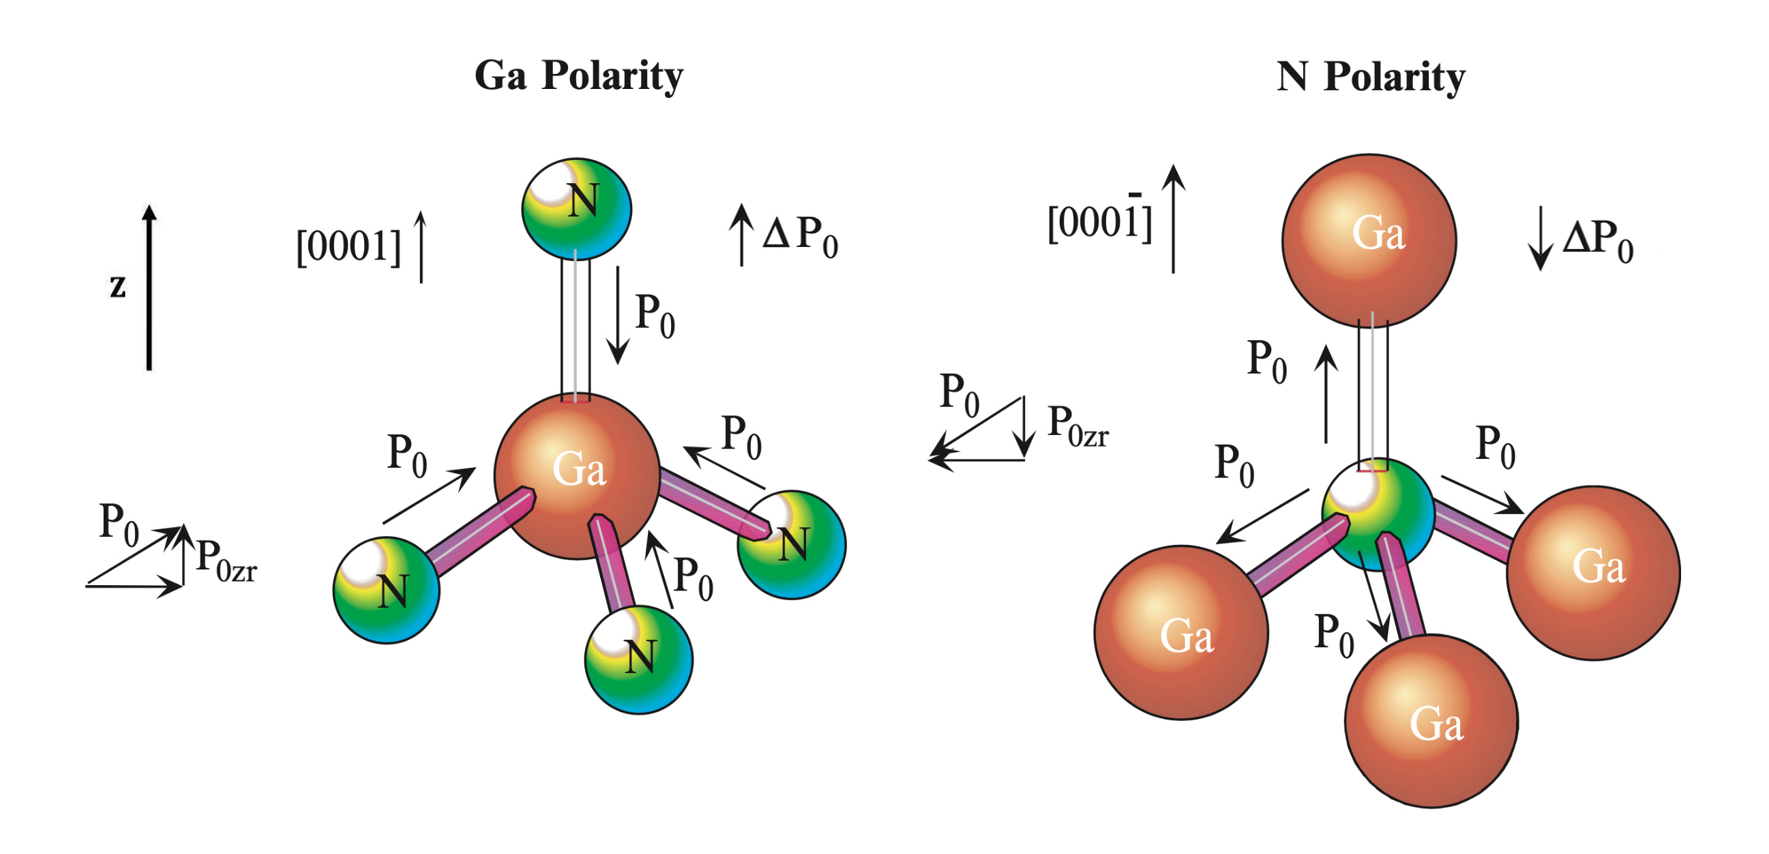
\includegraphics[width=0.9\textwidth]{ch2_3}
\caption[Ball and stick model of a GaN crystal for both Ga and N polarity with a homogeneous in-plane compressive strain]{Ball and stick model of a GaN crystal for both Ga and N polarity with a homogeneous in-plane compressive strain \protect\cite{morkoc2008polarization}}
\label{fig:2.3}
\end{figure}

\noindent GaN lattices, where $P_{0}$ denotes the pole between $Ga$ ions and $N$ ions vectorization. Take the GaN lattice with Ga polarity in the left figure as an example, since the electron cloud of the lattice is closer to the N atom, in the tetrahedral structure, the superposition of the \index{Polarization!vector} polarization vector $P_{0zr}$ in the $+z$ direction of the three bonds of the tetrahedral lattice cannot cancel it out. The polarization vector $P_{0}$ in the $-z$ direction, so the net polarization vector of the Ga-polar GaN lattice is along the $-z$ direction. The net polarization phenomenon in this lattice relaxation state is the spontaneous polarization \index{Spontaneous polarization} effect. However, when the Ga-polar GaN lattice is under uniform in-plane tensile strain, the accumulated polarization vector \index{Polarization!vector} in the $+z$ direction associated with the three bonds of the tetrahedral lattice decreases, thereby enhancing the net polarization vector along the $-z$ direction, as shown in \autoref{fig:2.2}. When there is in-plane uniform compressive strain in the Ga-polar GaN lattice, the cumulative polarization vector \index{Polarization!vector} in the $+z$ direction related to the three bonds of the tetrahedral lattice will increase, and the GaN lattice exhibits a net polarization vector along the $+z$ direction, as shown in \autoref{fig:2.3}. The change of the polarization vector in this external stress state is called the piezoelectric polarization \index{Piezoelectric!polarization} effect, and the change of net polarization vector of the lattice is the result of the combined action of the spontaneous polarization \index{Spontaneous polarization} and the piezoelectric polarization. In an N-polar GaN lattice, the same happens, except that the polarization direction is opposite to that of a Ga-polar GaN lattice \cite{morkoc2008polarization}.


\section{Piezoelectric theory of III-V nitrides}
\label{sec:Piezoelectric equations for III-V nitrides}
\subsection{Piezoelectric constitutive equation}
\label{sec:Piezoelectric constitutive equation}

According to the basic theory of piezoelectric \index{Piezoelectric!effect} effect, the stress-charge form of piezoelectric constitutive equation \index{Piezoelectric!constitutive equation} can be expressed as
\begin{equation}
\left\{\begin{array}{c}
\boldsymbol{\sigma}=\boldsymbol{c}_{E} \boldsymbol{S}-\boldsymbol{e}^{T} \boldsymbol{E} \\
\boldsymbol{D}=\boldsymbol{e} \boldsymbol{S}+\boldsymbol{k} E
\end{array}\right.
\label{eq:2.1}
\end{equation}
In this formula, $\boldsymbol{E}$ and $\boldsymbol{D}$ represent the electric \index{Electric!field} field strength vector and \index{Electric!displacement vector} electric displacement vector, and $\sigma$ is the stress tensor; $\boldsymbol{c}_{E}$ is the \index{Elastic!coefficient} elastic coefficient tensor; $\boldsymbol{e}$ is the linear piezoelectric \index{Piezoelectric!coefficient} coefficient; $\boldsymbol{k}$ is the dielectric constant tensor, and $\boldsymbol{S}$ is the strain \index{Strain} tensor.
Among them, the expression of linear \index{Piezoelectric!coefficient} piezoelectric coefficient $\boldsymbol{e}$ is
\begin{equation}
\boldsymbol{e}=\begin{bmatrix}
e_{11} & e_{12} & e_{13} & e_{14} & e_{15} & e_{16} \\
e_{21} & e_{22} & e_{23} & e_{24} & e_{25} & e_{26} \\
e_{31} & e_{32} & e_{33} & e_{34} & e_{35} & e_{36}
\end{bmatrix}
\label{eq:2.2}
\end{equation}
Next, we start to simplify the theoretical model. First, we only consider the condition of the external \index{Electric!field} electric field $\boldsymbol{E} = 0$. Therefore, \autoref{eq:2.1} can be simplified as
\begin{equation}
\left\{\begin{array}{c}
\boldsymbol{\sigma}=\boldsymbol{c}_{E} \boldsymbol{S}\\
\boldsymbol{D}=\boldsymbol{e} \boldsymbol{S}
\end{array}\right.
\label{eq:2.3}
\end{equation}
Since we only need to study the \index{Piezoelectric!polarization charge} piezoelectric polarization charge-strain \index{Strain} relationship, we only take $\boldsymbol{D}=\boldsymbol{e} \boldsymbol{S}$ for discussion, and the thin film \index{Thin film} materials we study are the III-V group nitride materials AlGaN, AlN and GaN with wurtzite \index{Wurtzite} structure. The linear piezoelectric \index{Piezoelectric!coefficient} coefficient $\boldsymbol{e}$ matrix has a special form, and its expansion is written in the matrix form as
\begin{equation}
\begin{bmatrix}
D_{x} \\
D_{y} \\
D_{z}
\end{bmatrix}=\begin{bmatrix}
0 & 0 & 0 & 0 & e_{15} & 0 \\
0 & 0 & 0 & e_{24} & 0 & 0 \\
e_{31} & e_{32} & e_{33} & 0 & 0 & 0
\end{bmatrix}\begin{bmatrix}
S_{x x} \\
S_{y y} \\
S_{z z} \\
S_{y z} \\
S_{x z} \\
S_{x y}
\end{bmatrix}
\label{eq:2.4}
\end{equation}
where $𝑒_{31} = 𝑒_{32}$. Since we only study the \index{Piezoelectric!polarization charge} piezoelectric polarization charge-strain \index{Strain} relationship in the $z$ direction, ie $D_{z}$, from \autoref{eq:2.4} we can get
\begin{equation}
\begin{aligned}
D_{z} &=e_{31} S_{x x}+e_{32} S_{y y}+e_{33} S_{z z} \\
&=e_{31}\left(S_{x x}+S_{y y}\right)+e_{33} S_{z z}
\end{aligned}
\label{eq:2.5}
\end{equation}
Therefore, the $z$-direction \index{Electric!displacement vector} electric displacement vector-strain \index{Strain} equation of III-V nitride \index{Nitride} materials is derived from the piezoelectric \index{Piezoelectric!constitutive equation} constitutive equation, where $S_{x x}$, $S_{y y}$, $S_{z z}$ are the strains of the material in the $x$, $y$, and $z$ directions, respectively.

\subsection{Piezoelectric polarization charge-strain equation}
\label{sec:Piezoelectric polarization-strain equation}

In electromagnetism, the electric displacement vector and electric polarization intensity are defined as:
\begin{equation}
\mathbf{D}=\varepsilon_{0} \mathbf{E}+\mathbf{P}
\label{eq:2.6}
\end{equation}
where $\mathbf{D}$ is the electric displacement \index{Electric!displacement vector} vector, $\varepsilon_{0}$ is the \index{Vacuum permittivity} vacuum permittivity, $\mathbf{E}$ is the electric field \index{Electric!field} strength, and $\mathbf{P}$ is the electric polarization \index{Electric!polarization strength} strength.

Since we only consider the condition of the external electric field \index{Electric!field} $\mathbf{E}=0$, and only consider the electric polarization in the z direction, \autoref{eq:2.6} can be simplified as:
\begin{equation}
D_{z}=P_{z}
\label{eq:2.7}
\end{equation}
Substituting it into \autoref{eq:2.5}, we finally get the \index{Piezoelectric!polarization charge} piezoelectric polarization charge-strain \index{Strain} equation in the $z$-direction of III-V nitride \index{Nitride} materials:
\begin{equation}
P_{z} =e_{31}\left(S_{x x}+S_{y y}\right)+e_{33} S_{z z}
\label{eq:2.8}
\end{equation}

Next, we discuss the physical meaning of \autoref{eq:2.8} in this study. The electric polarization \index{Electric!polarization strength} strength $\mathbf{P}$ (or electric polarization, or simply polarization) is the vector field that represents the density of permanent electric dipole moment \index{Electric!dipole moment} or induced electric dipole moment in the dielectric material, and is a physical quantity characterizing electric dipole moment in a material. In III-V nitride \index{Nitride} materials, the electric polarization $\mathbf{P}$ defined by \autoref{eq:2.8} can characterize the piezoelectric polarization \index{Piezoelectric!polarization} in the $z$ direction $P_{z}$ induced by \index{Strain} strain, so is usually represented by $P_{PE}$, \autoref{eq:2.8} is further rewritten for
\begin{equation}
P_{PE} =e_{31}\left(S_{x x}+S_{y y}\right)+e_{33} S_{z z}
\label{eq:2.9}
\end{equation}

So far, we have derived the mathematical equation for the relationship between piezoelectric polarization \index{Piezoelectric!polarization} and strain \index{Strain} in the $z$-direction of III-V nitride \index{Nitride} materials. When $P_{PE}< 0$, the polarization electric field \index{Polarization!electric field} in the material points to the negative direction of the $z$-axis, and is is directed from negative charges to positive charges. The distribution of piezoelectric polarization charges \index{Piezoelectric!polarization charge} is shown in \autoref{fig:2.4}. Conversely, when $P_{PE} > 0$, the polarization electric field in the material points in the positive z-axis direction, and the distribution of piezoelectric polarization charges is opposite to that in \autoref{fig:2.4}.

\begin{figure}[H] 
\centering    
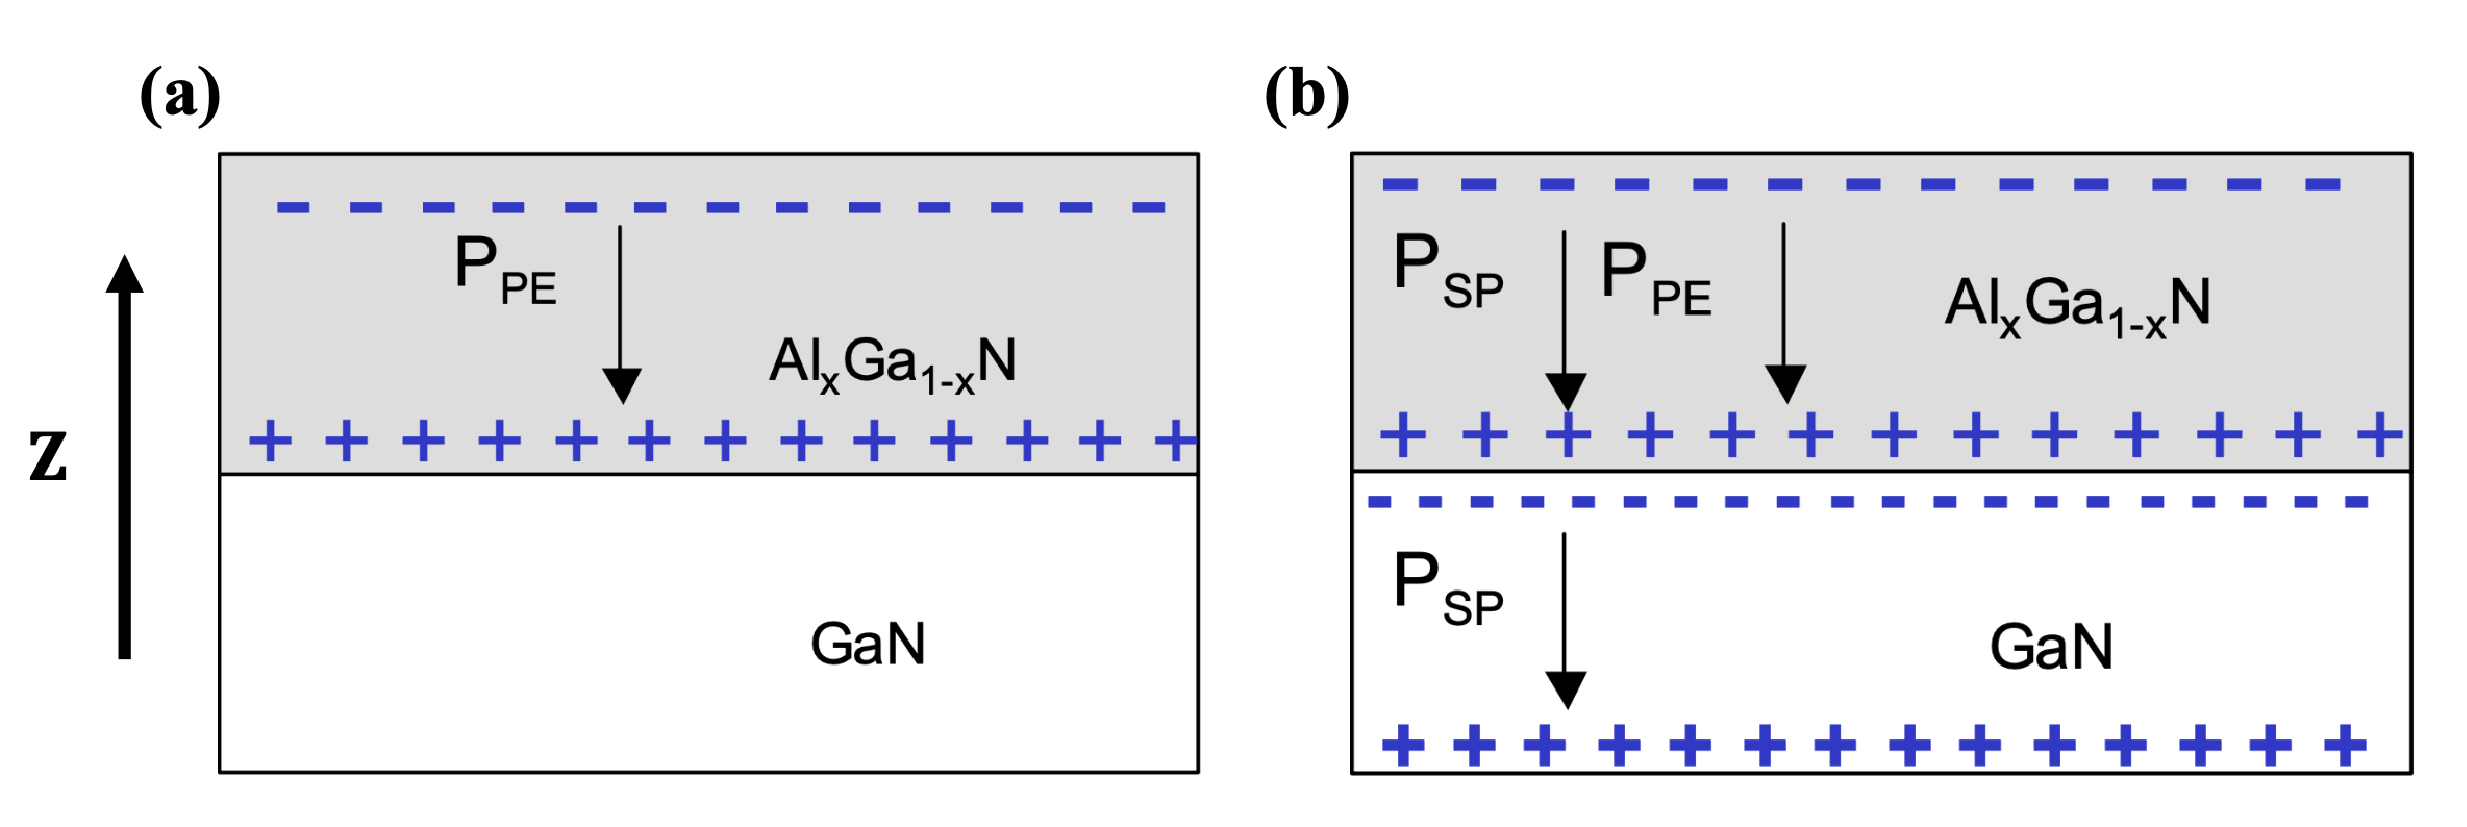
\includegraphics[width=0.9\textwidth]{ch2_4}
\caption[Piezoelectric polarization charge distribution of group III-V nitride material $Al_{x}Ga_{1-x}N$ when $P_{PE}<0$]{Piezoelectric polarization charge distribution of group III-V nitride material $Al_{x}Ga_{1-x}N$ when $P_{PE}<0$. (a) Spontaneous polarization charge is not considered. (b) Spontaneous polarization charge is considered \protect\cite{vetury2000polarization}}
\label{fig:2.4}
\end{figure}

\section{Lattice strain model of AlGaN/AlN/GaN heterojunction}
\label{sec:Lattice strain model of AlGaN/AlN/GaN heterojunction}

\subsection{Biaxial strain model of thin films}
\label{sec:Biaxial strain model of thin films}

In this section, we study the strains \index{Strain} of \index{AlGaN/AlN/GaN heterojunction} AlGaN/AlN/GaN heterojunction thin films \index{Thin film} in the $x$, $y$, and $z$ directions. The thicknesses of the AlGaN, AlN, and GaN films are 30 \unit{nm}, 1 \unit{nm}, and 4.3 \unit{um}, respectively. The thickness of the GaN film is much larger than AlGaN thin film \index{Thin film} and AlN thin film, and the GaN material is rigid. Therefore, we can approximately think that the GaN thin film is a rigid substrate \index{Substrate} material, and use the biaxial stress model \index{Biaxial stress model} to perform strain \index{Strain} analysis on the AlGaN thin film and the AlN thin film, as shown in \autoref{fig:2.5}. The thickness of the film material is much smaller than that of the rigid substrate, so when the film is subjected to lateral strain, the axial strain of the film can be calculated approximately through the Poisson's ratio \index{Poisson's!ratio} of the material:
\begin{equation}
S_{z}=-\frac{v}{1-v}\left(S_{x}+S_{y}\right)
\label{eq:2.10}
\end{equation}
where $S_{x}$, $S_{y}$, $S_{z}$ are the strains \index{Strain} in the $x$, $y$, and $z$ directions, respectively, and $v$ is the Poisson's ratio \index{Poisson's!ratio} of the thin film \index{Thin film} material.

\begin{figure}[H] 
\centering    
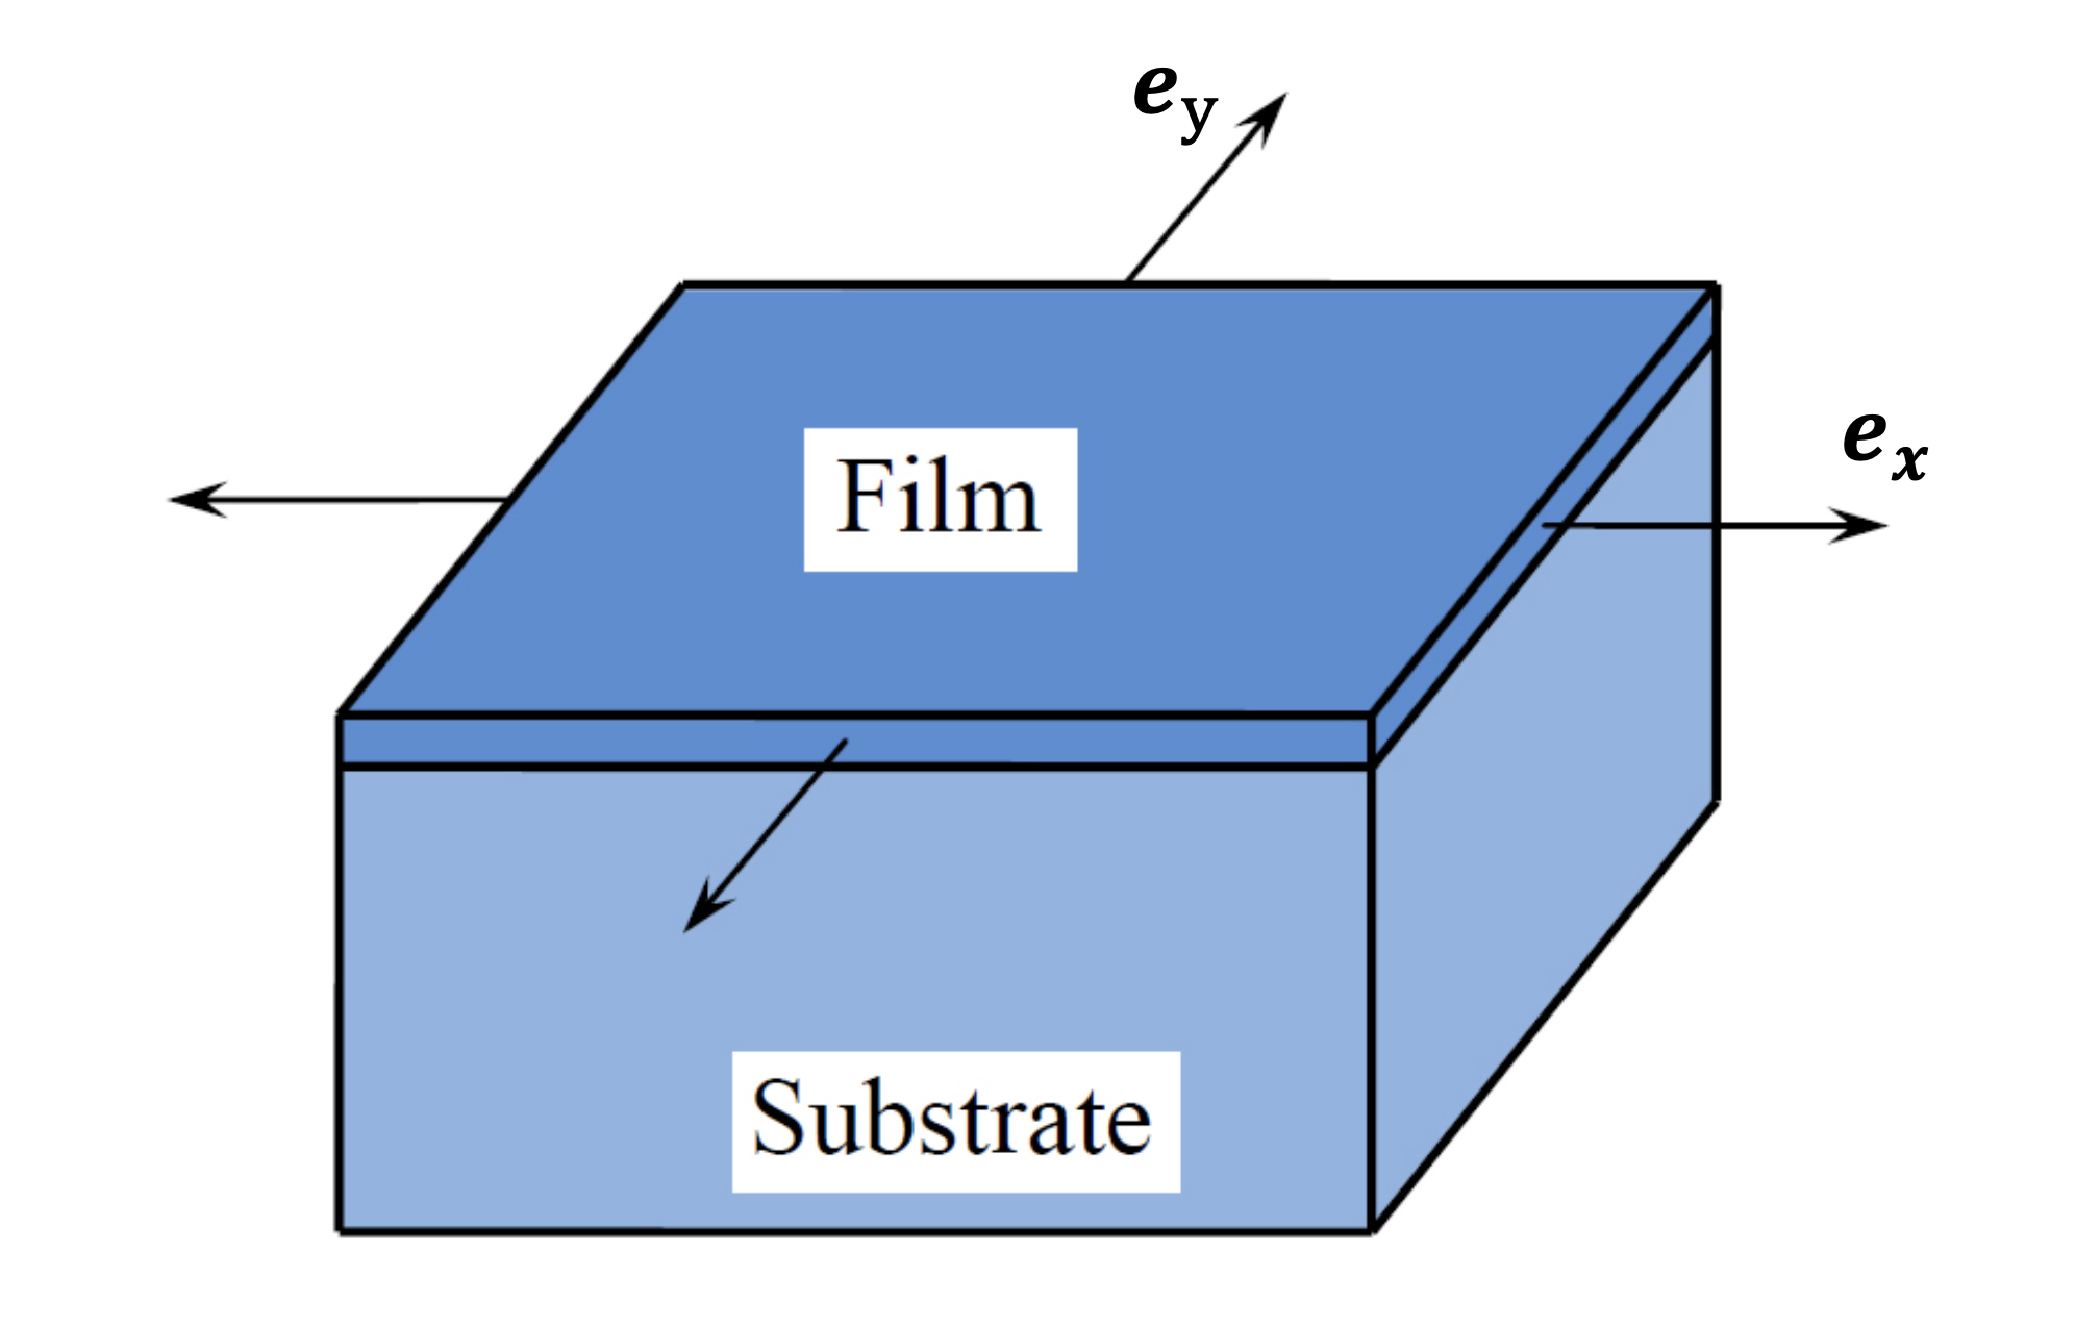
\includegraphics[width=0.6\textwidth]{ch2_5}
\caption[Schematic diagram of biaxial stress model]{Schematic diagram of biaxial stress model}
\label{fig:2.5}
\end{figure}

\subsection{Lattice strain in multilayer thin films}
\label{sec:Lattice strain in multilayer thin films}

Next we investigate the lattice strain \index{Lattice!strain} of the thin film \index{Thin film} due to \index{Lattice!mismatch} lattice mismatch. \autoref{fig:2.6} shows the relationship between the forbidden band width and lattice constant \index{Lattice!constant} of III-V nitride \index{Nitride} semiconductors at room temperature, where the lattice constant \index{Lattice!constant} of AlGaN (30$\%\;$Al) can be given by Vegard's law \index{Vegard's law} \cite{vegard1921konstitution,denton1991vegard}:
\begin{equation}
a_{\mathrm{Al}_{0.3} \mathrm{Ga}_{0.7 \mathrm{~N}}}=0.3 a_{\mathrm{AlN}}+0.7 a_{\mathrm{GaN}}
\label{eq:2.11}
\end{equation}
We can see that the lattice constants \index{Lattice!constant} of AlN crystal, AlGaN crystal and GaN crystal \index{Crystal} are inconsistent, and there is a certain lattice mismatch \index{Lattice!mismatch} between them. It is the lattice mismatch between the thin films \index{Thin film} in the \index{AlGaN/AlN/GaN heterojunction} AlGaN/AlN/GaN heterojunction that introduces strain \index{Strain} in the films, resulting in the corresponding piezoelectric polarization charge. It is also called lattice strain \index{Lattice!strain} because this strain is caused by lattice mismatch.

\begin{figure}[H] 
\centering    
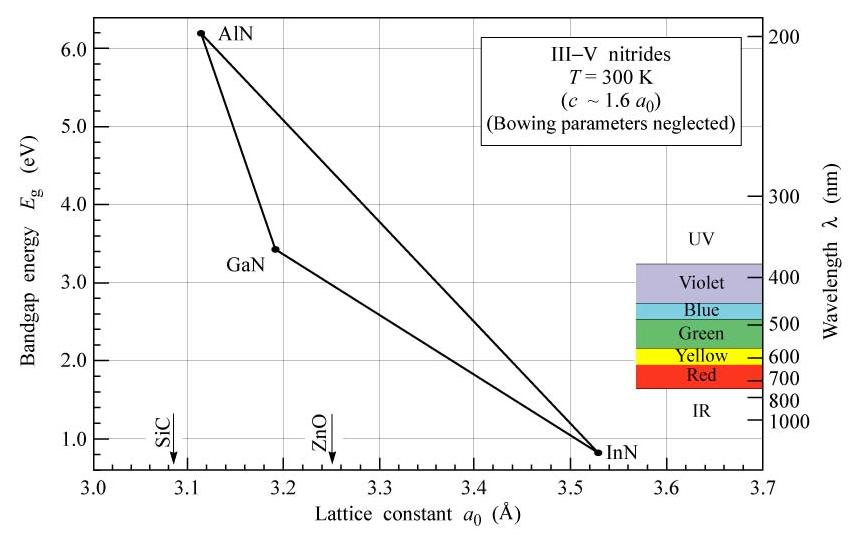
\includegraphics[width=0.9\textwidth]{ch2_6}
\caption[Bandgap energy versus lattice constant for III-V nitride semiconductors at room temperature
]{Bandgap energy versus lattice constant for III-V nitride semiconductors at room temperature}
\label{fig:2.6}
\end{figure}

The lattice strain \index{Lattice!strain} of the \index{Thin film} thin film is shown in \autoref{fig:2.7}. Due to the inconsistency of \index{Lattice!constant} lattice constants, crystals $A$ and $B$ have \index{Crystal} a certain lattice \index{Lattice!mismatch} mismatch. When the epitaxial layer \index{Epitaxial!layer} is composed of these two crystal materials, under ideal conditions (without considering the lattice-mismatched dislocations) there will be elastic strains \index{Elastic!strain} between lattices. Usually, since the thickness of the epitaxial substrate is much larger than that of the \index{Thin film} thin film, we approximately think that the lattice of the substrate \index{Substrate} does not produce \index{Elastic!strain} elastic strain, that is, the \index{Lattice!constant} lattice constant $a_{A}$ of the substrate $A$ does not change, and the lattice of the thin film $B$ undergoes \index{Elastic!deformation} elastic \index{Deformation} deformation. Thus, the deformed lattice constant \index{Lattice!constant} $a_{B}(epi)$ is equal to the lattice constant $a_{A}$ of the substrate $A$, that is, $a_{B}(epi)=a_{A}$. Then, the lateral lattice \index{Lattice!strain} strain $S_{B}$ of film $B$ is:
\begin{equation}
\begin{aligned}
S_{B} &=\frac{a_{B}(e p i)-a_{B}}{a_{B}} \\
&=\frac{a_{A}-a_{B}}{a_{B}}
\end{aligned}
\label{eq:2.12}
\end{equation}
In the ideal case of no external stress, the lateral $x$- and $y$-direction lattice strains \index{Lattice!strain} of film B are approximately the same, and the $z$-direction lattice strain \index{Lattice!strain} can be obtained according to the biaxial stress model \index{Biaxial stress model} (\autoref{eq:2.10}).

\begin{figure}[H] 
\centering    
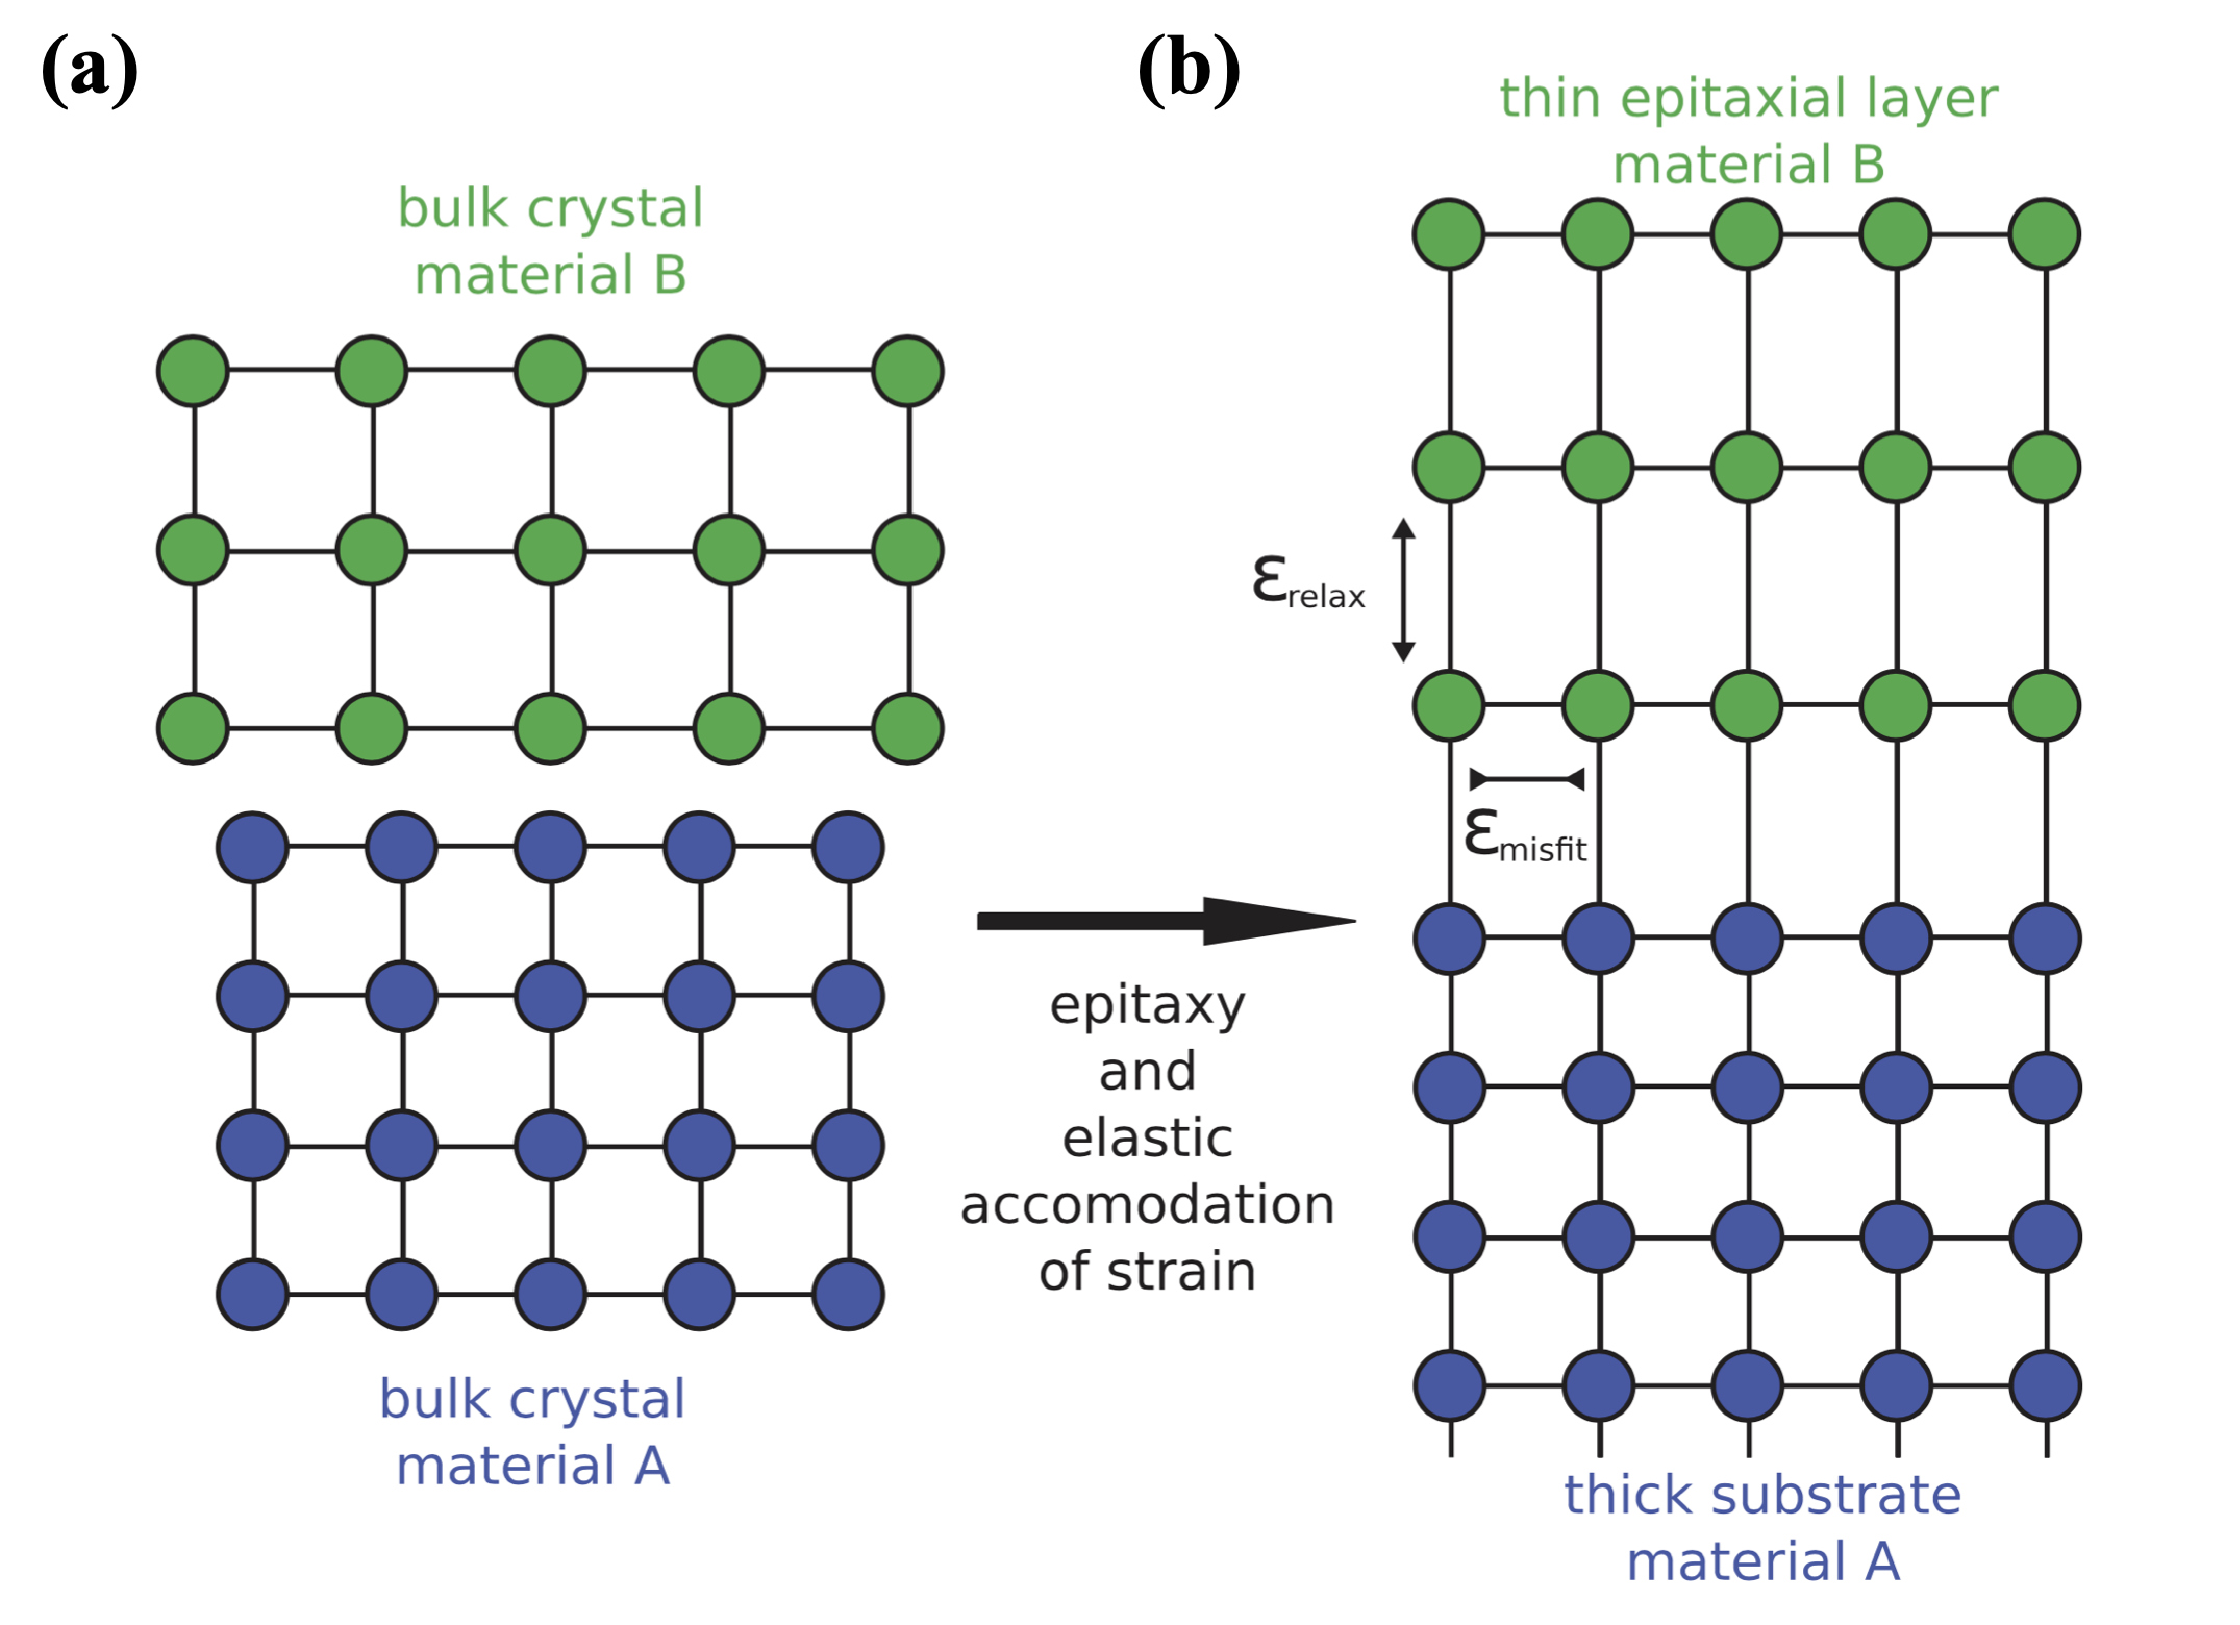
\includegraphics[width=0.9\textwidth]{ch2_7}
\caption[Lattice strain of the thin films]{Lattice strain of the thin films (a) Lattice mismatch between film and substrate material. (b) Purely elastic strain epitaxial layer without misfit dislocations \protect\cite{lopuszynski2012ordering}}
\label{fig:2.7}
\end{figure}

Similarly, considering the \index{AlGaN/AlN/GaN heterojunction} AlGaN/AlN/GaN heterojunction in this study and the thickness of each layer material (30 \unit{nm}/1 \unit{nm}/4.3 \unit{um}), the thickness of the GaN layer is much larger than that of the AlN film and the AlGaN film, We can approximate that GaN belongs to rigid substrate \index{Substrate} materials, and AlN and AlGaN belong to \index{Thin film} thin film materials. This is a structure consisting of two thin films, as shown in \autoref{fig:2.8}. It can be seen that since the lattice constants \index{Lattice!constant} of AlN crystal and AlGaN crystal \index{Crystal} are both smaller than those of GaN crystal, and the thickness of the GaN layer is much larger than that of the AlN film and the AlGaN film, the AlN film and AlGaN film are both subjected to tensile strain, and the lattice constants after deformation \index{Deformation} are all equal to lattice constants of GaN crystals.

\begin{figure}[H] 
\centering    
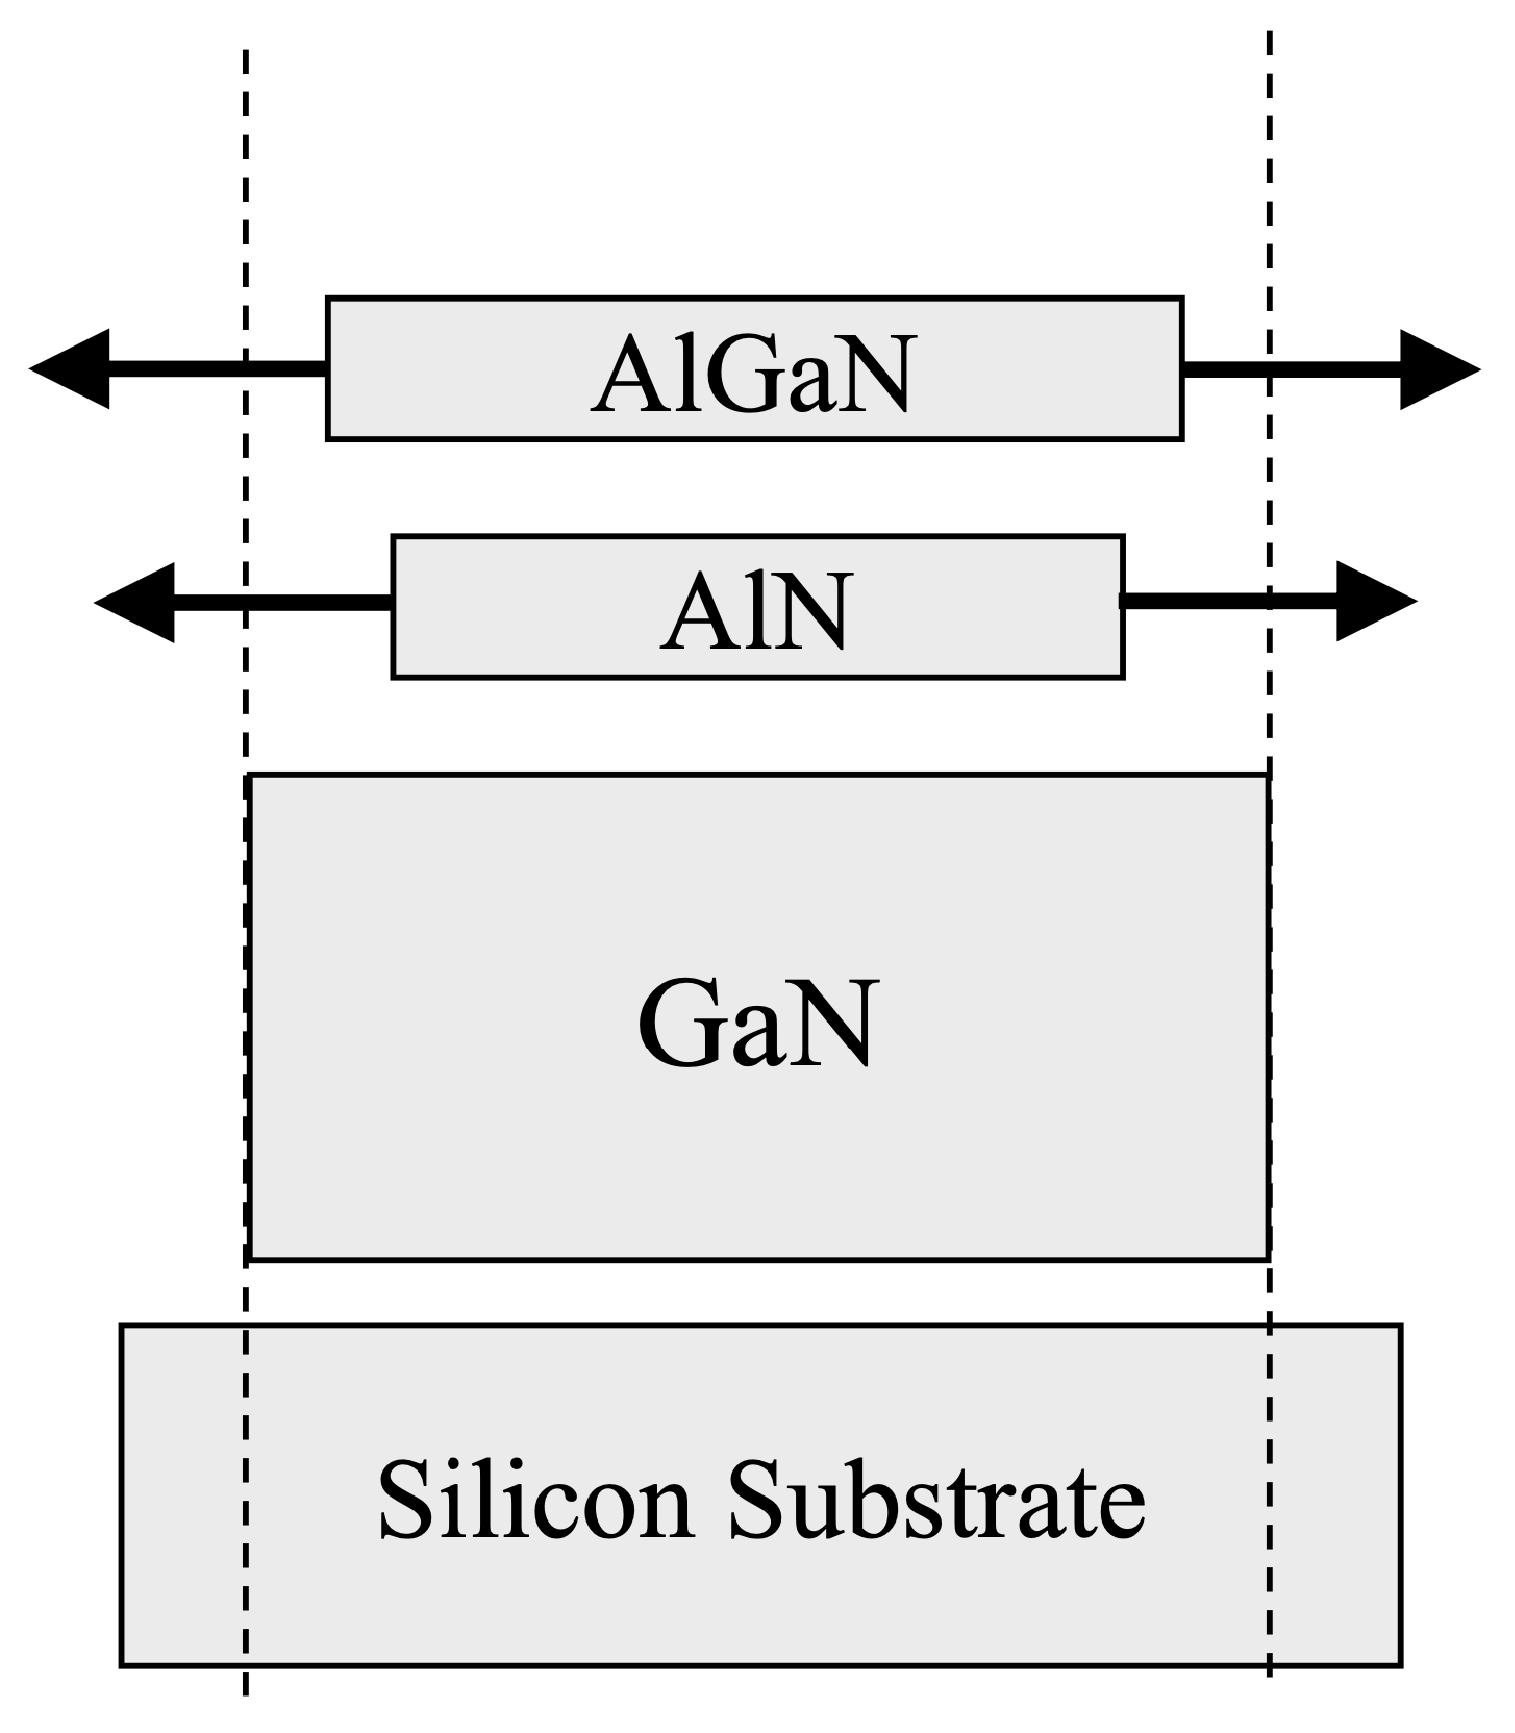
\includegraphics[width=0.6\textwidth]{ch2_8}
\caption[Thin film structure of AlGaN/AlN/GaN heterostructure]{Thin film structure of AlGaN/AlN/GaN heterostructure}
\label{fig:2.8}
\end{figure}

First we discuss the case where there is no external stress. In this case, the AlN film undergoes tensile \index{Elastic!strain} elastic strain, and its deformed lattice constant $a_{AlN}(epi)$ is equal to the lattice constant \index{Lattice!constant} $a_{GaN}$ of GaN, that is, $a_{AlN}(epi)=a_{GaN}$. Since the thickness of the AlN film is only 1 \unit{nm}, it can be reasonably approximated that the full lattice strain occurs in the AlN film. So the \index{Lattice!constant} lattice constant of the AlGaN film after deformation \index{Deformation} is equal to the lattice constant of the AlN film after the deformation, that is, $a_{AlGaN}(epi)=a_{AlN}(epi)$. Finally, we can approximately express the lateral lattice strain \index{Lattice!strain} of each layer of AlGaN/AlN/GaN \index{AlGaN/AlN/GaN heterojunction} heterojunction without external stress as follows:
\begin{equation}
S_{G a N}=\frac{a_{G a N}-a_{G a N}}{a_{G a N}}=0
\label{eq:2.13}
\end{equation}
\begin{equation}
S_{A l N}=\frac{a_{A l N}(e p i)-a_{A l N}}{a_{A l N}}=\frac{a_{G a N}-a_{A l N}}{a_{A l N}}
\label{eq:2.14}
\end{equation}
\begin{equation}
S_{AlGaN }=\frac{a_{A l G a N}(e p i)-a_{A l G a N}}{a_{A l G a N}}=\frac{a_{G a N}-a_{A l G a N}}{a_{A l G a N}}
\label{eq:2.15}
\end{equation}
In the ideal case of no external stress, the lattice deformations \index{Lattice!deformation} in the $x$ and $y$ directions of the AlN film and the AlGaN film are approximately the same, and the \index{Lattice!strain} lattice strain in the $z$ direction can be obtained according to the biaxial stress model \index{Biaxial stress model} described in \autoref{eq:2.10}.

In the presence of external stress, the lattice strain of each layer of \index{AlGaN/AlN/GaN heterojunction} AlGaN/AlN/GaN heterojunction will be more complicated. First, the GaN layer will deform laterally and longitudinally under the action of external stress, and the AlN film and AlGaN film will also deform accordingly. In this model, we approximately think that in the case of very weak external stress, each layer of the AlGaN/AlN/GaN heterojunction material still undergoes pure \index{Elastic!deformation} elastic \index{Deformation} deformation. The lattice constant \index{Lattice!constant} of the AlN film is still equal to that of the GaN layer, that is, the AlN film is still completely deformed. Therefore the lattice constant \index{Lattice!constant} of the deformed AlGaN film is still equal to that of the deformed AlN film. The mathematical expression is $a_{AlN}(starin)=a_{GaN}(starin)$, $a_{AlGaN}(starin)=a_{AlN}(starin)$. In this way, we can approximately express lateral lattice strain \index{Lattice!strain} of AlGaN/AlN/GaN heterojunction layers in the presence of external stress:
\begin{equation}
S_{G a N}(strain)=\frac{a_{G a N}(strain)-a_{G a N}}{a_{G a N}}
\label{eq:2.16}
\end{equation}
\begin{equation}
S_{A l N}(strain)=\frac{a_{A l N}(strain)-a_{A l N}}{a_{A l N}}=\frac{a_{G a N}(strain)-a_{A l N}}{a_{A l N}}
\label{eq:2.17}
\end{equation}
\begin{equation}
S_{AlGaN }(strain)=\frac{a_{A l G a N}(strain)-a_{A l G a N}}{a_{A l G a N}}=\frac{a_{G a N}(strain)-a_{A l G a N}}{a_{A l G a N}}
\label{eq:2.18}
\end{equation}

\begin{table}[H]
\renewcommand\arraystretch{1.5}
\centering
\caption[Physical parameters of wurtzite structure AlN and GaN]{Physical parameters of wurtzite structure AlN and GaN}
\setlength{\tabcolsep}{7mm}{
\begin{tabular}{cccc}
\hline \hline
Parameters                    & AlN     & GaN    & Ref           \\ \hline \hline
Lattice constant a (\unit{nm})     & 0.311   & 0.319  & \cite{vurgaftman2003band}     \\
Lattice constant c (\unit{nm})     & 0.498   & 0.519  & \cite{vurgaftman2003band}     \\
Bandgap $E_{g}$ (\unit{eV})        & 6.25    & 3.510  & \cite{vurgaftman2003band}     \\
Effective mass (Electron)     & 0.32    & 0.20   & \cite{vurgaftman2003band}     \\
Effective mass (Hole)         & 3.53    & 1.56   & \cite{bernardini1997spontaneous}     \\
Relative permittivity         & 8.5     & 10.4   & \cite{bernardini1997spontaneous}     \\
C11 (\unit{GPa})                   & 396     & 390    & \cite{vurgaftman2003band}     \\
C12 (\unit{GPa})                   & 137     & 145    & \cite{vurgaftman2003band}     \\
C13 (\unit{GPa})       			  & 108     & 106    & \cite{vurgaftman2003band}     \\
C33 (\unit{GPa})       			  & 373     & 398    & \cite{vurgaftman2003band}     \\
e31 (\unit{\coulomb\per\square\m})               & -0.58   & -0.452 & \cite{morkoc2008polarization,stevens2013thermo} \\
e33 (\unit{\coulomb\per\square\m})     		  & 1.55    & 0.818  & \cite{morkoc2008polarization,stevens2013thermo} \\
e311 (\unit{\coulomb\per\square\m})   			  & 5.850   & 6.185  & \cite{pal2011second}     \\
e333 (\unit{\coulomb\per\square\m})   			  & -10.750 & -8.090 & \cite{pal2011second}     \\
e133 (\unit{\coulomb\per\square\m})   			  & 4.533   & 1.543  & \cite{pal2011second}     \\
$P_{sp}$ (\unit{\coulomb\per\square\m})   			  & -0.081  & -0.029 & \cite{pal2011second}     \\ \hline \hline
\end{tabular}}
\label{tab:2.1}
\end{table}

\noindent In addition, under the action of external stress, the lattice deformations \index{Lattice!deformation} in the $x$ and $y$ directions of the GaN layer, AlN thin film, and AlGaN thin film \index{Thin film} may be different. Therefore, we can use the finite element analysis \index{Finite element analysis} method to calculate the \index{Strain} strain in the $x$, $y$ and $z$ directions of the GaN layer under the action of external stress according to the principles of material mechanics, and then calculate the $x$ and $y$ direction lattice constant \index{Lattice!constant} according to \autoref{eq:2.16}. On this basis, the lattice strains \index{Lattice!strain} in the $x$ and $y$ directions of the AlN film and the AlGaN film are solved respectively according to \autoref{eq:2.17} and \autoref{eq:2.18}. Finally, the lattice strain \index{Lattice!strain} in $z$ direction of the AlN film and the AlGaN film can be solved according to the biaxial \index{Biaxial stress model} stress model.

\subsection{Piezoelectric polarization charge of GaN AlGaN AlN layer}
\label{sec:Piezoelectric polarization charge of GaN AlGaN AlN layer}

In this subsection, we study the lattice strain \index{Lattice!strain} of the active region \index{Active region} of the \index{Cantilever} cantilevered GaN layer under the action of external stress using the methods of finite element \index{Finite element analysis} analysis. On this basis, the lattice strain and piezoelectric polarization charge \index{Piezoelectric!polarization charge} of GaN AlGaN AlN layer can be further obtained.

 According to the principles of material mechanics, we can solve the strain \index{Strain} of the cantilevered GaN under different external stresses through the methods of finite element analysis. \autoref{fig:2.9} shows the deformation \index{Deformation} of the GaN cantilever under 4 \unit{\mN} external stress simulated by COMSOL Multiphysics 5.1. The length, width, and height of the cantilever are 350 \unit{\um}, 60 \unit{\um}, and 4.3 \unit{\um}, respectively. The Poisson's ratio \index{Poisson's!ratio} and Young's modulus \index{Young's modulus} of the GaN material are 0.2 \cite{qin2017mechanical} and 290 \unit{GPa} \cite{ben2014young,nowak1999elastic} respectively. The external stress is applied to the front half of the \index{Cantilever} cantilever, and we set up a sampling point to extract the strain of the HEMT's active area.

\begin{figure}[H] 
\centering    
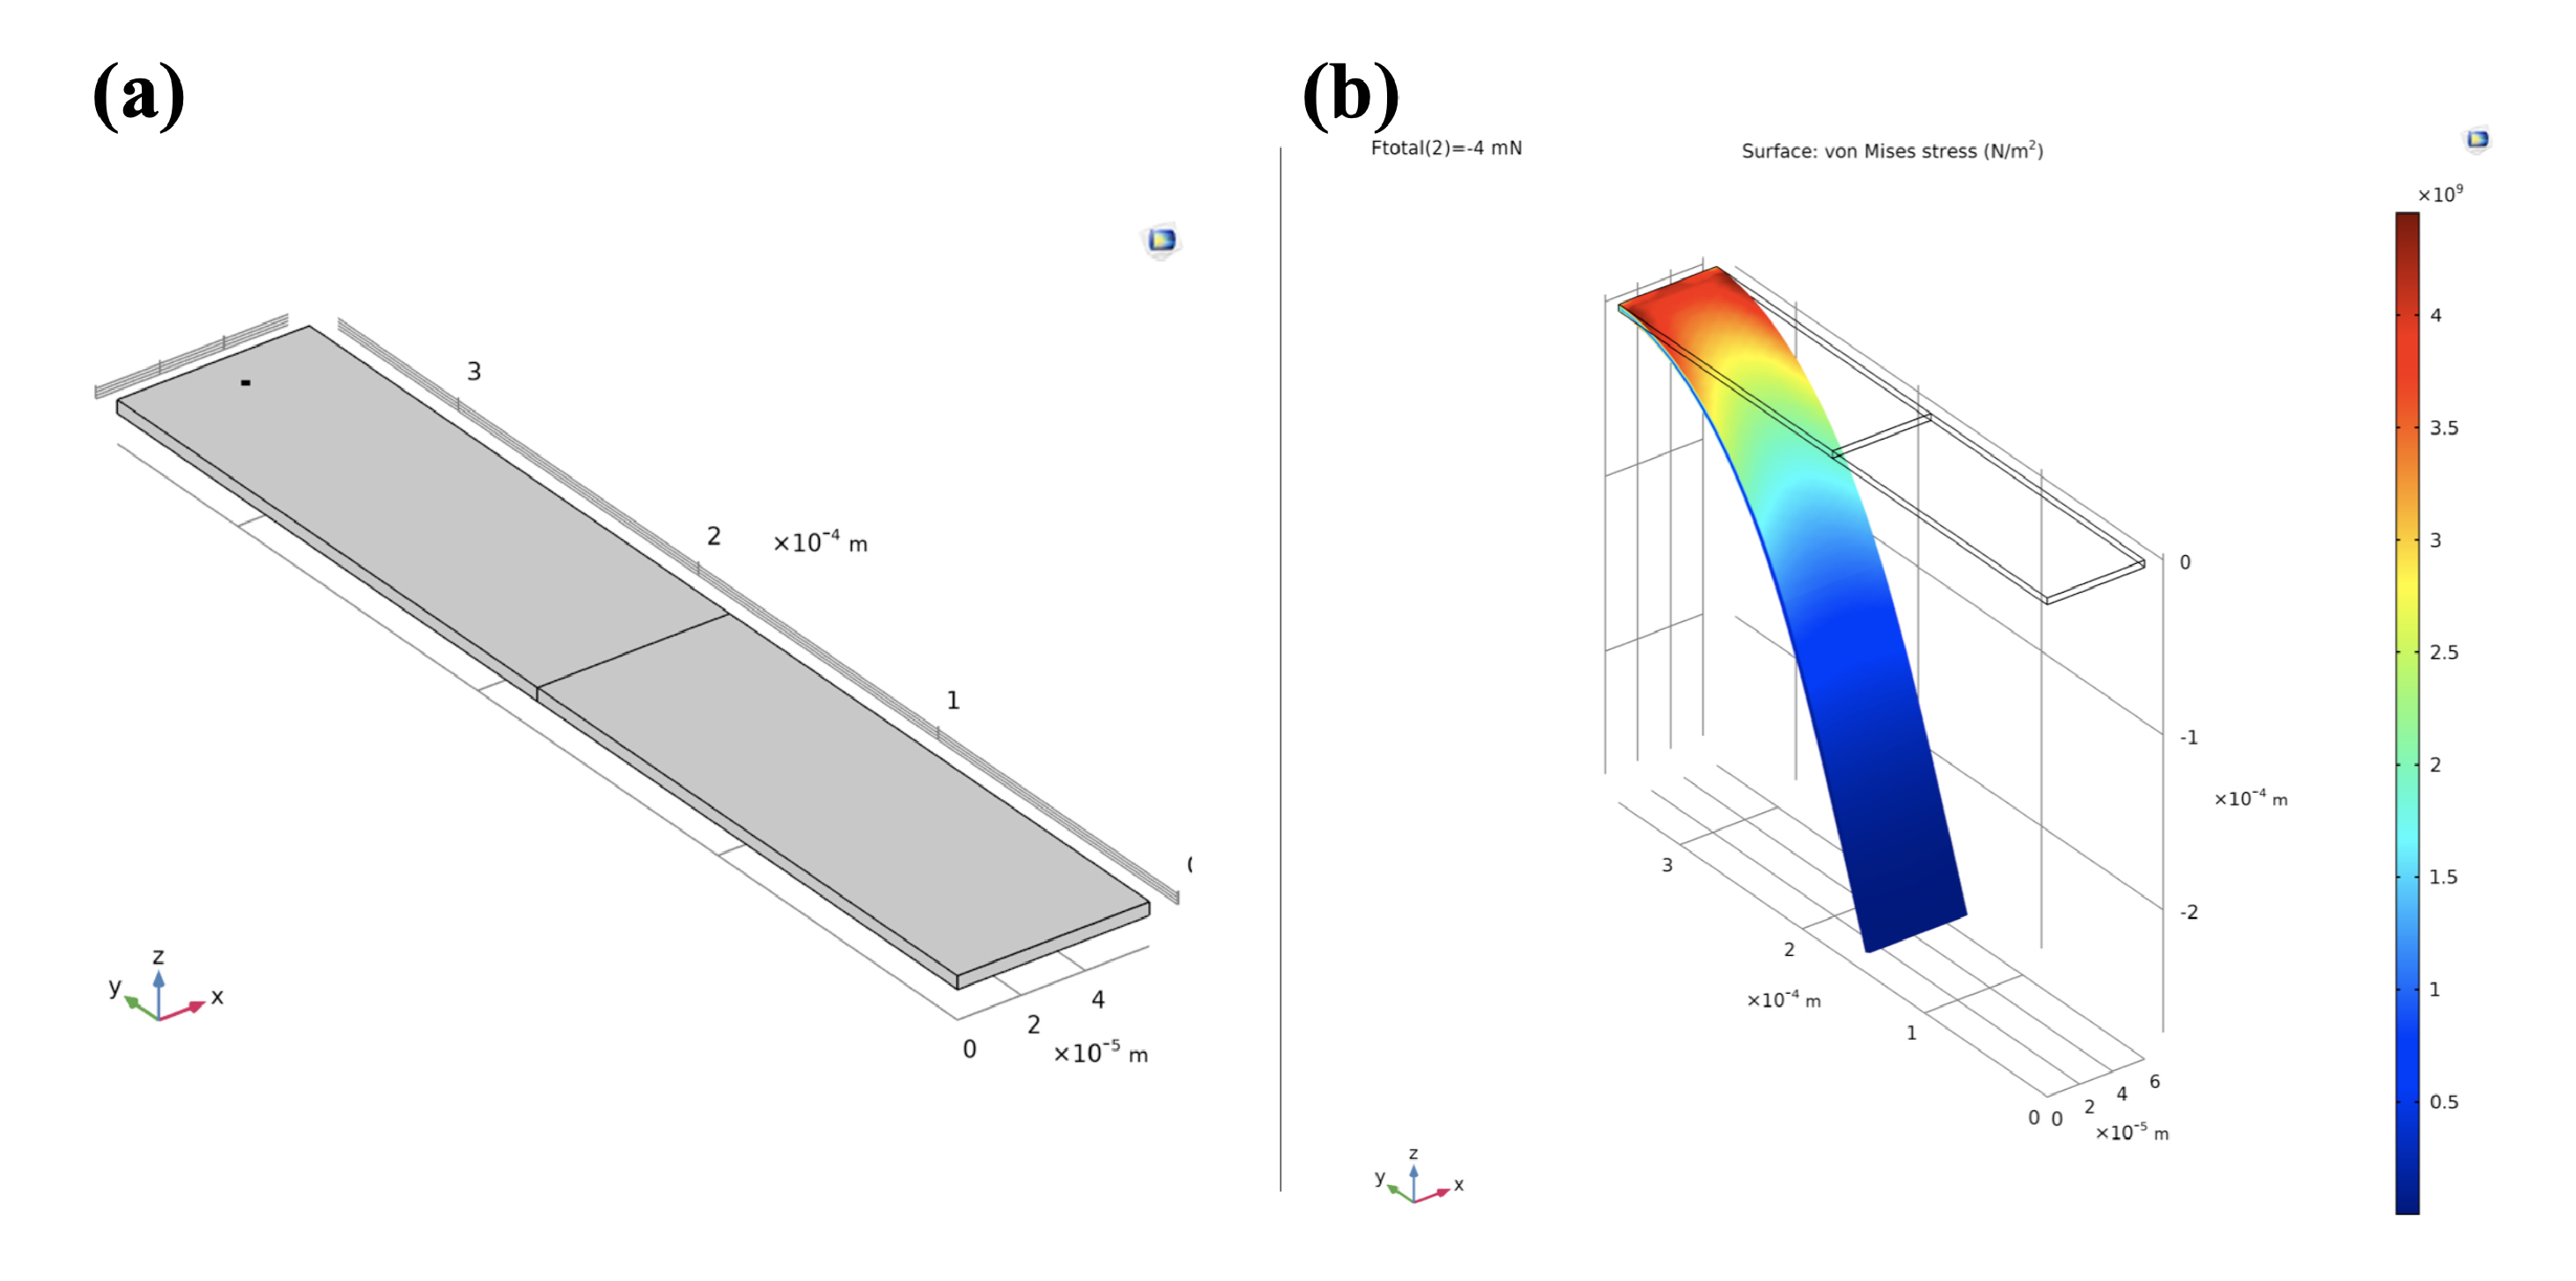
\includegraphics[width=0.9\textwidth]{ch2_9}
\caption[Finite element analysis of GaN cantilever strain under external stress]{Finite element analysis of GaN cantilever strain under external stress (a) Structure of the GaN cantilever. (b) Deformation of the GaN cantilever under 4 \unit{\mN} external stress.}
\label{fig:2.9}
\end{figure}

We take the theoretical calculation of the MPD \index{Magnetosensory power MEMS devices (MPD)} device in \autoref{ch:Magnetosensory Power Devices} in this thesis as an example. \autoref{fig:2.9}a is a schematic diagram of the structure of the \index{Cantilever} GaN cantilever, which is the same as that of the MPD cantilever. \autoref{fig:2.9}b shows the Von Mises stress \index{Von Mises stress} distribution of the GaN cantilever under 4 \unit{\mN} external stress. It can be seen that due to the special structure of the cantilever, the Von Mises stress at the fixed end of the cantilever is much larger than other regions, which is exactly the active region \index{Active region} of \index{AlGaN/AlN/GaN heterojunction} AlGaN/AlN/GaN heterojunction. So we verify that lattice strain \index{Lattice!strain} induced by external stress can be enlarged by the cantilever structure. By applying a downward normal force of 0 $\sim$ 24 \unit{\mN} to the front half of the cantilever, we calculated the GaN lattice strain \index{Lattice!strain} in the active region \index{Active region} corresponding to different external stresses. The calculation results are shown in \autoref{tab:2.2}. We can clearly see that under the action of external stress, the lattice strain in the $x$-direction of the active region is very small and almost negligible, while the lattice strain in the $y$-direction and $z$-direction is significant. Therefore, through the finite element analysis \index{Finite element analysis} model of material mechanics, we obtained the GaN's lattice strains in the $x$, $y$ and $z$ directions of \index{HEMT} cantilevered HEMT's active region under different external stresses, namely $𝑆_{xx}(GaN)$, $𝑆_{yy}(GaN)$ and $𝑆_{zz}(GaN)$. On this basis, the piezoelectric polarization charge \index{Piezoelectric!polarization charge} densities of GaN ($P_{GaN}^{PE}$), AlN ($P_{AlN}^{PE}$) and AlGaN ($P_{AlGaN}^{PE}$) thin films \index{Thin film} are further deduced, as shown in \autoref{tab:2.2}.

\begin{table}[]
\renewcommand\arraystretch{1.5}
\centering
\caption[Lattice strain of GaN cantilever active region and the corresponding piezoelectric polarization charge density of the films at 0 $\sim$ 24 \unit{\mN} downward force]{Lattice strain of GaN cantilever active region and the corresponding piezoelectric polarization charge density of the films at 0 $\sim$ 24 \unit{\mN} downward force}
\begin{tabular}{ccccccc}
\hline \hline
\multirow{2}{*}{\begin{tabular}[c]{@{}c@{}}F \\ (\unit{\mN})\end{tabular}} &
  \multirow{2}{*}{\begin{tabular}[c]{@{}c@{}}Strain tensor,\\ $S_{xx}$\end{tabular}} &
  \multirow{2}{*}{\begin{tabular}[c]{@{}c@{}}Strain tensor,\\ $S_{yy}$\end{tabular}} &
  \multirow{2}{*}{\begin{tabular}[c]{@{}c@{}}Strain tensor,\\ $S_{zz}$\end{tabular}} &
  \multicolumn{3}{c}{\begin{tabular}[c]{@{}c@{}}Piezoelectric polarization \\ charge densities (\unit{\coulomb\per\square\m})\end{tabular}} \\
    &            &           &            & $P_{GaN}^{PE}$  & $P_{AlN}^{PE}$  & $P_{AlGaN}^{PE}$  \\ \hline \hline
0   & 0          & 0         & 0          & 0       & -0.0492 & -0.0092 \\
-4  & -0.0001688 & 0.0148460 & -0.0036991 & -0.0097 & -0.0637 & -0.0200 \\
-8  & 0.0000291  & 0.0220201 & -0.0055929 & -0.0145 & -0.0710 & -0.0254 \\
-12 & 0.0001830  & 0.0268448 & -0.0068830 & -0.0178 & -0.0760 & -0.0291 \\
-16 & 0.0003008  & 0.0305848 & -0.0078887 & -0.0204 & -0.0798 & -0.0320 \\
-20 & 0.0003956  & 0.0337095 & -0.0087319 & -0.0226 & -0.0830 & -0.0344 \\
-24 & 0.0004726  & 0.0363812 & -0.0094546 & -0.0244 & -0.0857 & -0.0364 \\ \hline \hline
\end{tabular}
\label{tab:2.2}
\end{table}

So far, we have constructed a theoretical model of the \index{Piezoelectric!polarization charge} piezoelectric polarization charge intensity - external stress relationship ($P_{PE} - F$) of \index{MEMS} MEMS devices based on AlGaN/AlN/AlGaN \index{AlGaN/AlN/GaN heterojunction} heterojunction cantilever \index{Cantilever} structure. By combining piezoelectric constitutive \index{Piezoelectric!constitutive equation} equations, biaxial stress model \index{Biaxial stress model} and \index{Finite element analysis} finite element analysis, we can mathematically solve the piezoelectric polarization charge intensities of GaN ($P_{GaN}^{PE}$) layer, AlN ($P_{AlN}^{PE}$) layer and AlGaN ($P_{AlGaN}^{PE}$) layer when the cantilever is subjected to different external stresses $F$. The change of the piezoelectric polarization charge intensity $P_{PE}$ will affect the electrical properties of the heterojunction. In \autoref{sec:Self-consistent coupling model of strained AlGaN/AlN/GaN heterojunction}, we will study the modulation \index{Modulation} properties of the piezoelectric polarization charge intensity $P_{PE}$ on the AlGaN/AlN/AlGaN heterojunction energy \index{Energy band} band, carrier \index{Carrier!distribution} distribution, and 2DEG concentration \index{Two-dimensional electron gas (2DEG)} through a self-consistent coupled computational \index{Self-consistent computational model} model.

\section{Self-consistent coupling model of strained AlGaN/AlN/GaN heterojunction}
\label{sec:Self-consistent coupling model of strained AlGaN/AlN/GaN heterojunction}

\subsection{The theoretical equations of the model}
\label{sec:The theoretical equations of the model}

The physical model of the energy band \index{Energy band} of the \index{AlGaN/AlN/GaN heterojunction} AlGaN/AlN/GaN heterojunction is a semi-classical model based on the Schrödinger equation \index{Schrödinger equation} and the \index{Poisson's!equation} Poisson's equation. Under the effective mass approximation, the electron subband in the growth direction of the AlGaN/AlN/GaN heterojunction is the solution of the stationary Schrödinger equation \cite{lenka2011self}
\begin{equation}
-\frac{\hbar^{2}}{2} \frac{d}{d x}\left[\frac{1}{m^{*}} \frac{d \psi_{i}(x)}{d x}\right]+\left[V(x)-E_{i}\right] \psi_{i}(x)=0
\label{eq:2.19}
\end{equation}
where $m^{*}$ represents the effective mass of the electron at the edge of the conduction \index{Conduction band} band, $V(x)$ represents the potential energy, $E_{i}$ represents the energy of the ith subband, and $\psi_{i}(x)$ represents the wave function of the ith subband. Ignoring the non-parabolicity of the conduction band, we assume that  $m^{*}$ is independent of electron energy, which is isotropic and has abrupt changes at the interface \index{Interface} between AlGaN, AlN, and GaN.

The expression for potential \index{Potential!energy} energy $V(x)$ is:
\begin{equation}
\mathrm{V}(x)=V_{c}(x)+V_{h}(x)+V_{x c}(x)
\label{eq:2.20}
\end{equation}
where $V_{c}(x)$ represents the conduction band edge potential in the form of a step function related to the conduction band shift at the AlGaN/AlN/GaN heterojunction, and $V_{h}(x)$ is the Hartree potential \index{Hartree potential} induced by electrostatic interactions \index{Electrostatic!interactions} due to the distribution of mobile and stationary charges. $V_{x c}(x)$ is the exchange-correlated potential of many-body interactions that are not included in the \index{Hartree potential} Hartree potential \cite{lee2002self}.

$V_{h}(x)$ is the solution of the \index{Poisson's!equation} Poisson's equation:
\begin{equation}
\frac{d}{d x}\left[\varepsilon(x) \frac{d V_{h}(x)}{d x}\right]=-q \varphi(x)
\label{eq:2.21}
\end{equation}
where $\varepsilon(x)$ is the dielectric constant of the material with abrupt changes at the interface \index{Interface} between AlGaN, AlN and GaN. $q$ is the absolute value of the unit charge.

The total charge density distribution $\varphi(x)$ is given by:
\begin{equation}
\varphi(x)=\sum_{j=t, i, b} \sigma(x) \delta\left(x-x_{i}\right)+p(x)+N_{D}^{+}(x)-n(x)-N_{A}^{-}
\label{eq:2.22}
\end{equation}
where $\sigma(x)$ is the density of polarization charges \index{Polarization!charge} at the interface between AlGaN, AlN and GaN, $p(x)$ and $n(x)$ are the concentrations of holes and free electrons, respectively, and $N_{D}^{+}$ is the donor ion concentration, $N_{A}^{-}$ is the acceptor ion concentration.

According to the electrical neutrality \index{Electrical!neutrality condition} condition, this formula also must be satisfied in the AlGaN/AlN/GaN \index{AlGaN/AlN/GaN heterojunction} heterojunction interval:
\begin{equation}
\int_{x_{t}}^{x_{p}} \rho(x) d x=0
\label{eq:2.23}
\end{equation}
Written in the form of the sum of all charges:
\begin{equation}
\int_{x_{t}}^{x_{p}}\left[p(x)+N_{D}^{+}(x)-n(x)-N_{A}^{-}\right] d x=0
\label{eq:2.24}
\end{equation}
The carrier concentration \index{Carrier!concentration} distribution \index{Carrier!distribution} in the AlGaN/AlN/GaN heterojunction is given by:
\begin{equation}
n(x)=\sum_{i} n_{i}\left|\psi_{i}(x)\right|^{2}
\label{eq:2.25}
\end{equation}
where $n_{i}$ is the density of electrons in the ith subband, and usually expressed as a function of effective mass:
\begin{equation}
\mathrm{n}_{i}=\frac{m^{*} k_{B} T}{\pi \hbar^{2}} \ln \left[1+\exp \left(\frac{E_{F}-E_{i}}{k_{B} T}\right)\right]
\label{eq:2.26}
\end{equation}
$k_{B}$ and $T$ are Boltzmann constant and electron temperature, respectively.

The two-dimensional electron gas (2DEG) \index{Two-dimensional electron gas (2DEG)} areal density $N_{e}$ is equal to the sum of the electron densities in all the subbands of the heterojunction:
\begin{equation}
N_{e}=\int_{x_{t}}^{x_{b}} n(x) d x=\sum_{i} n_{i}
\label{eq:2.27}
\end{equation}

Next, we study the coupling of the \index{Piezoelectric!polarization charge} piezoelectric polarization charge intensity $P_{PE}$ under external \index{Strain} strain derived earlier into a self-consistent computational model \index{Self-consistent computational model} through the Poisson's equation \index{Poisson's!equation} of \autoref{eq:2.21}. Due to the non-centrosymmetric wurtzite \index{Wurtzite} crystal \index{Crystal} structure, there are two types of intrinsic polarizations in \index{AlGaN/AlN/GaN heterojunction} AlGaN/AlN/GaN heterojunctions \cite{ambacher1999two-b}: (i) spontaneous polarization \index{Spontaneous polarization} existing in AlGaN ($P_{AlGaN}^{sp}$), AlN ($P_{AlN}^{sp}$) and GaN ($P_{GaN}^{sp}$); (ii) piezoelectric polarization \index{Piezoelectric!polarization} due to lattice strain present in GaN ($P_{GaN}^{PE}$), AlN ($P_{AlN}^{PE}$) and AlGaN ($P_{AlGaN}^{PE}$). The density of polarization charges \index{Polarization!charge} at the \index{Interface} interface $P_{interface}$ of AlGaN, AlN and GaN can be expressed as:
\begin{equation}
P_{\text {Interface }}=P_{s p}+P_{P E}+e_{311} S_{\|}^{2}+e_{333} S_{\perp}^{2}+e_{313} S_{\|} S_{\perp}
\label{eq:2.28}
\end{equation}
where $P_{s p}$ is the spontaneous polarization charge intensity, $P_{P E}$ is the piezoelectric polarization charge intensity \index{Piezoelectric!polarization charge} induced by \index{Lattice!strain} lattice strain, and $e_{ijk}$ is the nonlinear \index{Piezoelectric!coefficient} piezoelectric coefficient. $S_{\perp}$ and $S_{\|}$ are the lattice strains perpendicular to c-plane and parallel to the c-plane induced by external stress, respectively. In this model, we only consider the piezoelectric polarization \index{Piezoelectric!polarization} effect in the linear case, so \autoref{eq:2.28} can be simplified as:
\begin{equation}
P_{\text {Interface }}=P_{s p}+P_{P E}
\label{eq:2.29}
\end{equation}
\autoref{eq:2.29} is the polarization charge density in the total charge density distribution of \autoref{eq:2.22}. The spontaneously polarized charge intensity of AlGaN (30$\%$ Al) can be given by \index{Vegard's law} Vegard's law \cite{vegard1921konstitution,denton1991vegard}:
\begin{equation}
P_{A l_{x} G a_{1-x} N}^{s p}=x P_{A l N}^{s p}+(1-x) P_{G a N}^{s p}-b_{A l_{x} G a_{1-x} N} x(1-x)
\label{eq:2.30}
\end{equation}
where $x$ is the percentage of Al composition in AlGaN and $b_{A l_{x} G a_{1-x} N}$ is the bending coefficient of AlGaN \cite{morkoc2008polarization}.

The above are the basic physics equations required to numerically solve the energy band \index{Energy band} of AlGaN/AlN/GaN heterojunction \index{AlGaN/AlN/GaN heterojunction} under external \index{Strain} strain \cite{morkoc2008polarization,lenka2011self,lenka20142deg,jiang2018thesis}.



\subsection{A self-consistent numerical method for one-dimensional Schrödinger-Poisson coupling equation}
\label{sec:A self-consistent numerical method for one-dimensional Schrodinger-Poisson coupling equation}

The analytical solution of the Schrödinger-Poisson coupling equation \index{Schrödinger-Poisson coupling equation} is difficult to derive, so it is usually solved by self-consistent \index{Self-consistent computational model} coupling numerical calculation using finite difference or finite element mathematical methods \cite{lenka2011self,lenka20142deg}, as shown in \autoref{fig:2.10}. First, we input the potential energy \index{Potential!energy} $V_{in}(x)$ as the initial iteration, and calculate the wave function $\psi_{i}(x)$ and the corresponding eigenenergy $E_{i}$ using the steady-state Schrödinger wave equation (\autoref{eq:2.19}), and then use the \autoref{eq:2.25} and \autoref{eq:2.16} to calculate the electron density $n_{i}$ and the carrier concentration distribution \index{Carrier!concentration} $n(x)$ in the subband. The Hartree potential \index{Hartree potential} $V_{h}(x)$ is further calculated in the Poisson's equation \index{Poisson's!equation} using the given donor concentration $N^{+}_{D}(x)$, acceptor concentration $N_{A}^{-}$, and polarization charge density \index{Polarization!charge} at the \index{Interface} interface $\sigma(x)$, and the potential \index{Potential!energy} energy $V_{x}$ is also calculated according to \autoref{eq:2.20}. Then We substitute the obtained potential energy $V_{x}$ at this time into the steady-state Schrodinger wave equation to find the new wave function $\psi_{i}(x)$ and the corresponding eigenenergy $E_{i}$, and to solve the new carrier concentration distribution $n(x)$. This new $n(x)$ together with the donor concentration and acceptor concentration can be used to calculate the new Hartree potential \index{Hartree potential} $V_{h}(x)$ and new potential energy \index{Potential!energy} $V_{x}$ in the \index{Poisson's!equation} Poisson's equation. Compare the newly obtained potential energy $V_{x}$ with the previous result, and if it is outside the error range, continue to iterate until convergence is achieved. Finally, the self-consistent solutions of $V_{x}$ and $n(x)$ are used to further determine the \index{Energy band} energy band diagram and the carrier concentration \index{Carrier!concentration} of the \index{AlGaN/AlN/GaN heterojunction} AlGaN/AlN/GaN heterojunction.

\begin{figure}[H] 
\centering    
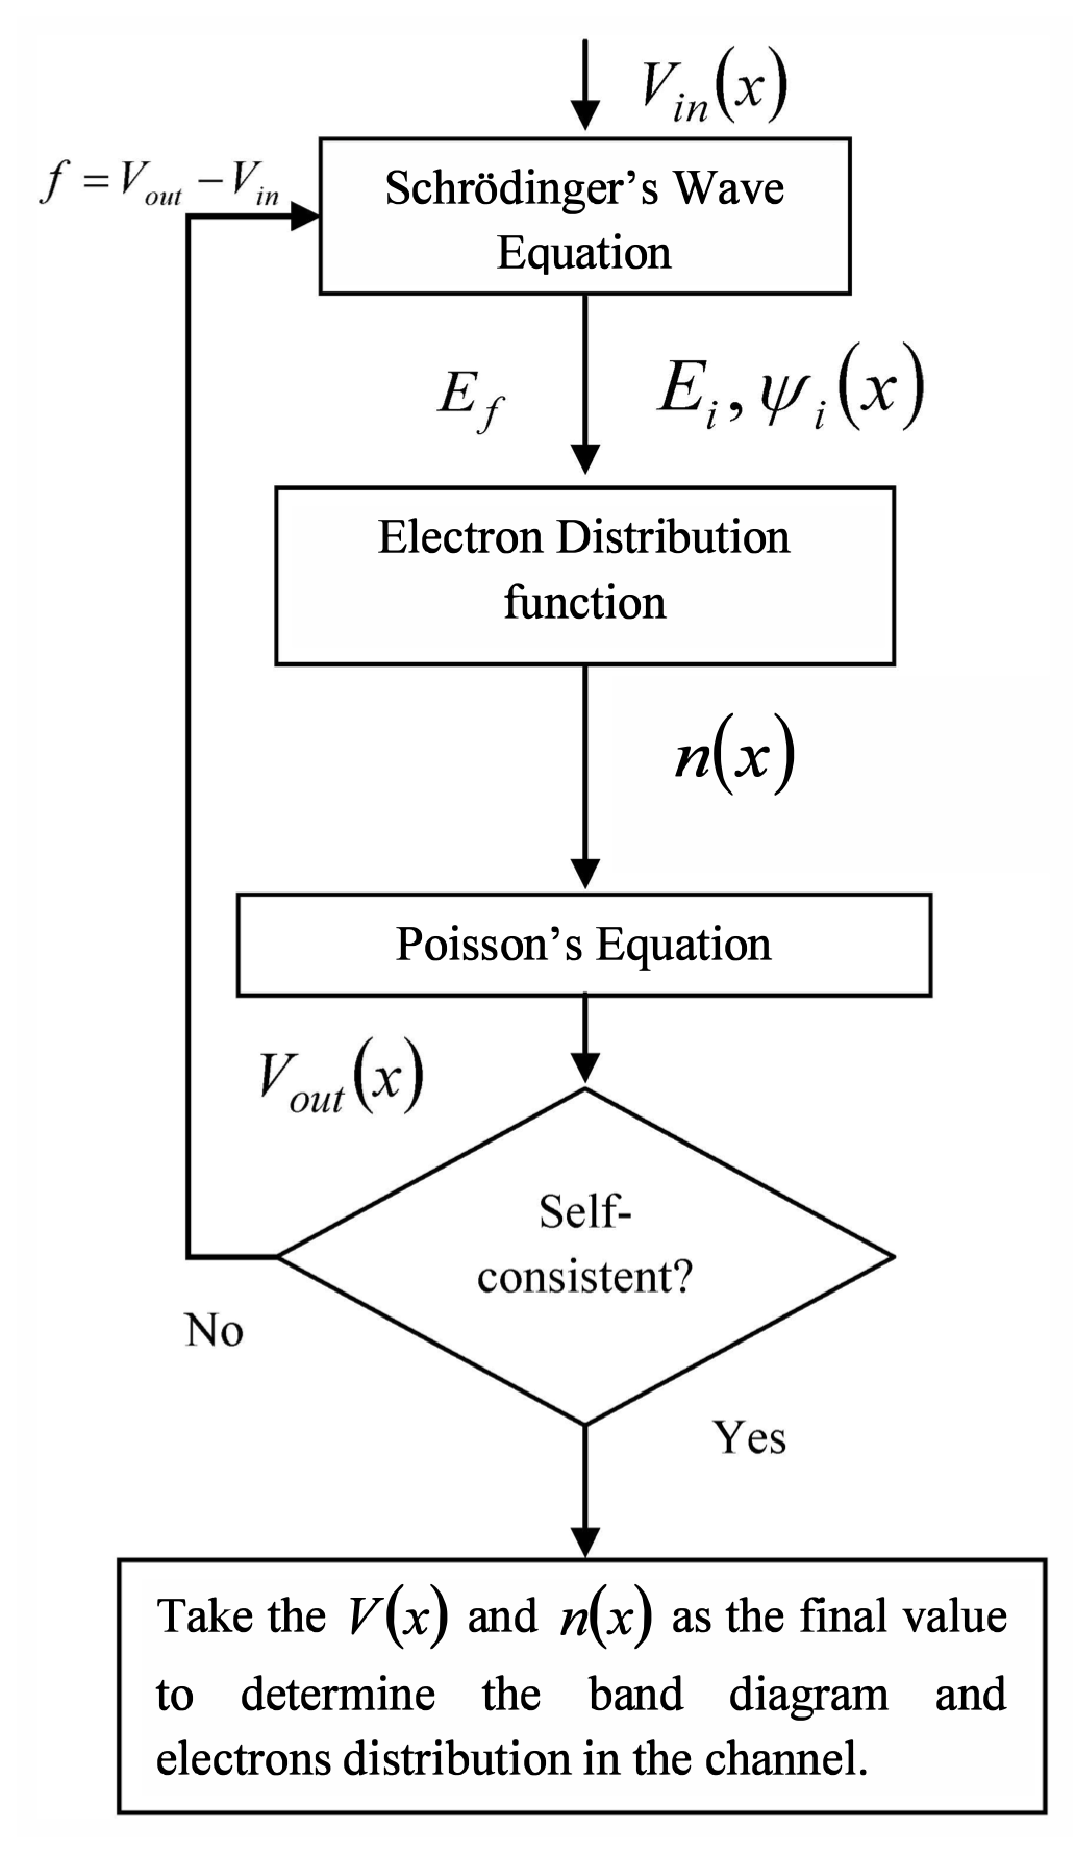
\includegraphics[width=0.6\textwidth]{ch2_10}
\caption[Iteration process of Schrodinger-Poisson self-consistent calculation]{Iteration process of Schrodinger-Poisson self-consistent calculation \protect\cite{lenka20142deg}}
\label{fig:2.10}
\end{figure}

\section{The framework of theoretical model}
\label{sec:The framework of theoretical model}

\begin{figure}[H] 
\centering    
\includegraphics[width=0.9\textwidth]{ch2_11}
\caption[Framework diagram of the theoretical model]{Framework diagram of the theoretical model}
\label{fig:2.11}
\end{figure}

So far, we have constructed a complete theoretical model of the MEMS device based on the \index{AlGaN/AlN/GaN heterojunction} AlGaN/AlN/AlGaN heterojunction cantilever \index{Cantilever} structure. By combining the piezoelectric constitutive \index{Piezoelectric!constitutive equation} equation, the biaxial stress model \index{Biaxial stress model} and the finite element \index{Finite element analysis} analysis, we deduce the mathematical relationship between the piezoelectric polarization charge intensity \index{Piezoelectric!polarization charge} and the external stress. Through the self-consistent coupling calculation model \index{Self-consistent computational model} of the AlGaN/AlN/GaN heterojunction, we further solved the modulation \index{Modulation} effect of the piezoelectric polarization charge intensity at the interface on the heterojunction energy band \index{Energy band} and the electron-hole wave function, thus successfully constructing a semi-classical physical model to explain the regulation mechanism \index{Physical!mechanism} of external stress on the electrical properties of MEMS devices. The overall framework \index{Physical!framework} of the theoretical model is shown in \autoref{fig:2.11}. The piezoelectric polarization charge density \index{Piezoelectric!polarization charge} at the interface is effectively modulated by external stress, thereby changing the electrostatic field \index{Electrostatic!field} in the \index{AlGaN/AlN/GaN heterojunction} AlGaN/AlN/GaN heterojunction, and finally modulating the heterojunction energy band, electron-hole wave function and carrier \index{Carrier!distribution} distribution. This model is an approximate semi-classical physical model with series of simplifications and approximations, which successfully reveals the modulation \index{Modulation} characteristics of piezotronics \index{Piezotronics} effect on MEMS \index{MEMS} devices based on AlGaN/AlN/AlGaN heterojunction cantilever \index{Cantilever} structure.

\section{Simulation results of theoretical model}
\label{sec:Simulation results of theoretical model}

In the above theoretical analysis, we mainly take the theoretical modeling of MEMS under the downward force as an example to illustrate the method. Theoretical modeling and analysis of upward forces is similar. Different from the previous downward stress situation, the upward force on the cantilever \index{Cantilever} weakens the electrical performance of MEMS, that is, the reaction will increase the potential well at the AlN/GaN \index{Interface} interface, thereby reducing the concentration of \index{Two-dimensional electron gas (2DEG)} 2DEG. \autoref{tab:2.3} shows the lattice strain \index{Lattice!strain} of GaN cantilever \index{Cantilever} active region \index{Active region} and the corresponding piezoelectric polarization charge density \index{Piezoelectric!polarization charge} of the films at 0 $\sim$ 24 \unit{\mN} upward force. The corresponding simulation results of \index{Magnetosensory power MEMS devices (MPD)} MPD is in \autoref{fig:ch2_MPD_theory_up}.

\begin{table}[H]
\renewcommand\arraystretch{1}
\centering
\caption[Lattice strain of GaN cantilever active region and the corresponding piezoelectric polarization charge density of the films at 0 $\sim$ 24 \unit{\mN} upward force]{Lattice strain of GaN cantilever active region and the corresponding piezoelectric polarization charge density of the films at 0 $\sim$ 24 \unit{\mN} upward force}
\begin{tabular}{ccccccc}
\hline \hline
\multirow{2}{*}{\begin{tabular}[c]{@{}c@{}}F \\ (\unit{\mN})\end{tabular}} &
  \multirow{2}{*}{\begin{tabular}[c]{@{}c@{}}Strain tensor,\\ $S_{xx}$\end{tabular}} &
  \multirow{2}{*}{\begin{tabular}[c]{@{}c@{}}Strain tensor,\\ $S_{yy}$\end{tabular}} &
  \multirow{2}{*}{\begin{tabular}[c]{@{}c@{}}Strain tensor,\\ $S_{zz}$\end{tabular}} &
  \multicolumn{3}{c}{\begin{tabular}[c]{@{}c@{}}Piezoelectric polarization \\ charge densities (\unit{\coulomb\per\square\m})\end{tabular}} \\
    &            &           &            & $P_{GaN}^{PE}$  & $P_{AlN}^{PE}$  & $P_{AlGaN}^{PE}$  \\ \hline \hline
0   & 0          & 0         & 0          & 0       & -0.0492 & -0.0092 \\
4  & 0.0003518 & -0.0152836 & 0.0037110 & 0.0099 & -0.0340 & 0.0021 \\
8  & 0.0002443  & -0.0226277 & 0.0055619 & 0.0148 & -0.0267 & 0.0076 \\
12 & 0.0001342  & -0.0274473 & 0.0067851 & 0.0180 & -0.0219 & 0.0111 \\
16 & 0.0000447  & -0.0311016 & 0.0077137 & 0.0204 & -0.0183 & 0.0138 \\
20 & -0.0000288  & -0.0341114 & 0.0084785 & 0.0224 & -0.0153 & 0.0161 \\
24 & -0.0000895  & -0.0366690 & 0.0091278 & 0.0240 & -0.0128 & 0.0179 \\ \hline \hline
\end{tabular}
\label{tab:2.3}
\end{table}


\begin{figure}[H] 
\centering    
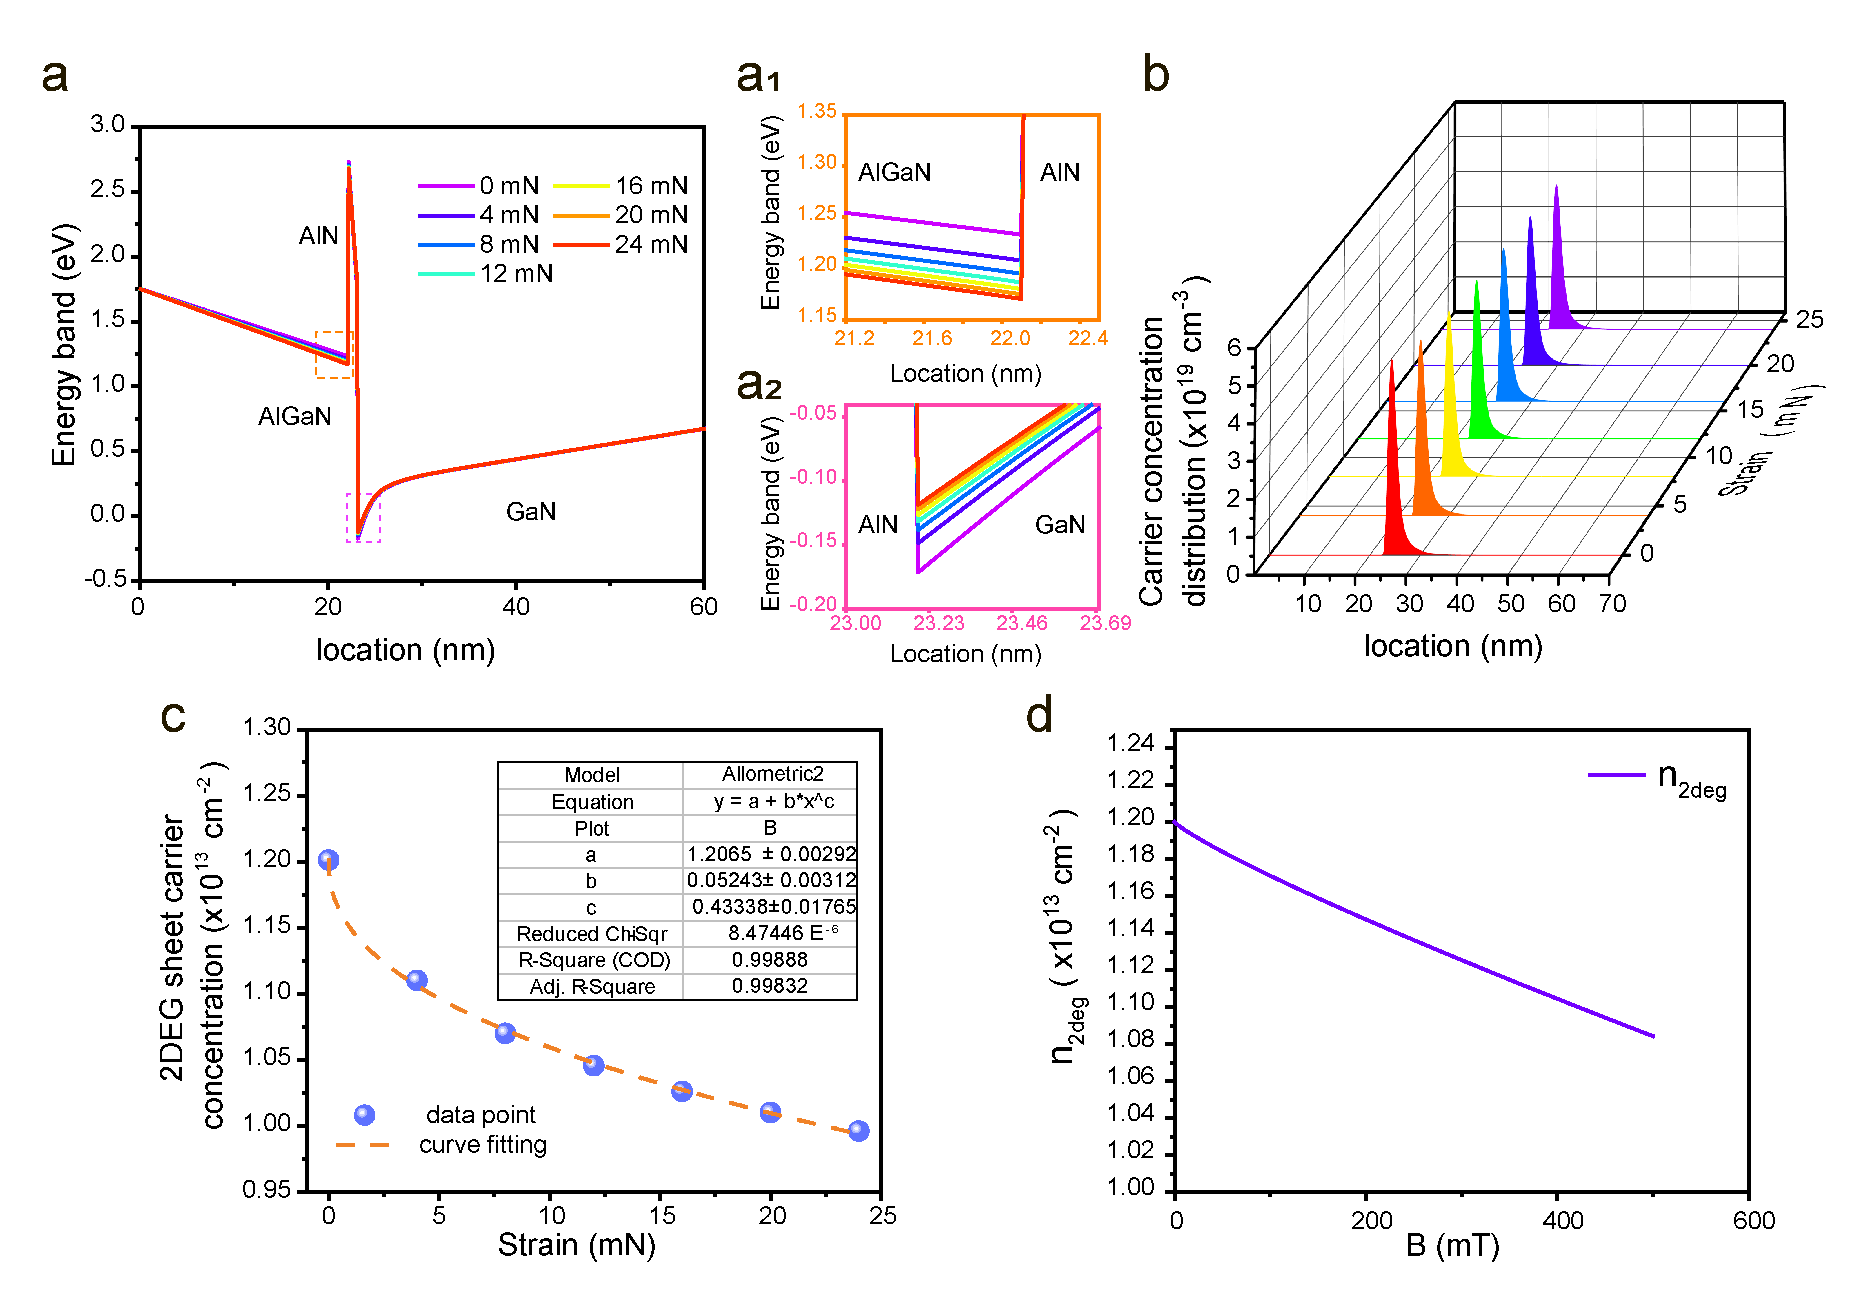
\includegraphics[width=0.88\textwidth]{ch2_MPD_theory_up}
\caption[Simulation results of MPD with upward magnetic force]{Simulation results of MPD with upward magnetic force}
\label{fig:ch2_MPD_theory_up}
\end{figure}

\begin{figure}[H] 
\centering    
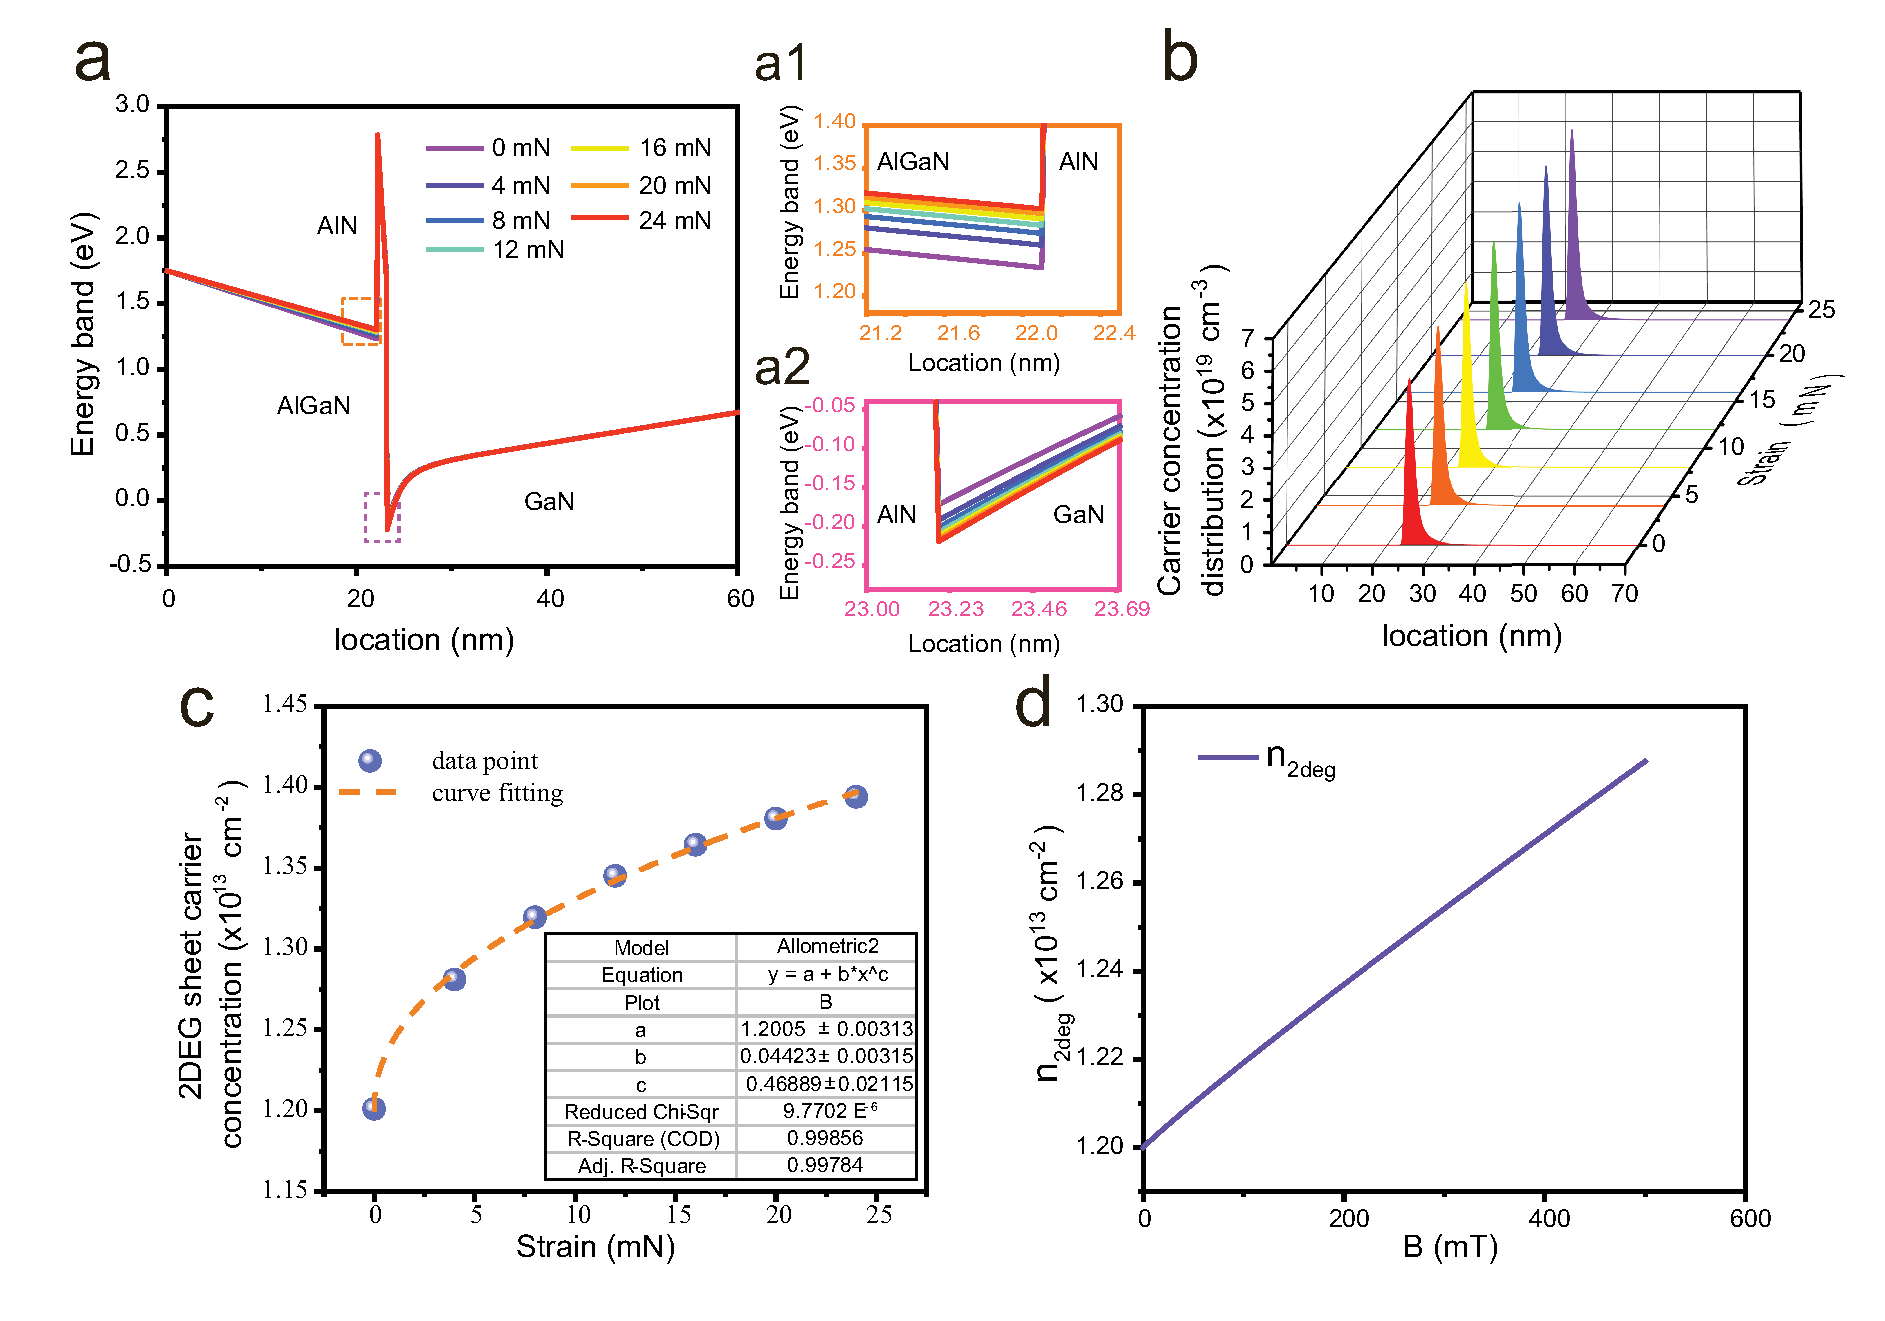
\includegraphics[width=0.88\textwidth]{ch2_MPD_theory_down}
\caption[Simulation results of MPD with downward magnetic force]{Simulation results of MPD with downward magnetic force}
\label{fig:ch2_MPD_theory_down}
\end{figure}


\begin{figure}[H] 
\centering    
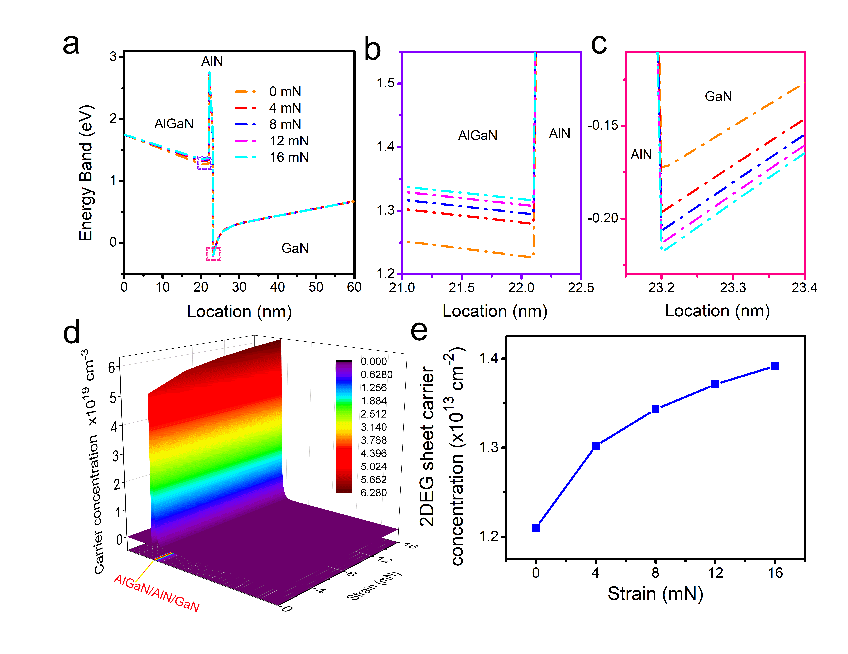
\includegraphics[width=0.9\textwidth]{ch2_SPD_theory}
\caption[Simulation results of SPD with downward normal force]{Simulation results of SPD with downward normal force}
\label{fig:ch2_SPD_theory}
\end{figure}


We also present the theoretical simulation results of the \index{Strain-controlled power MEMS devices
(SPD)} SPD and MPD \index{Magnetosensory power MEMS devices (MPD)} at downward force, as shown in \autoref{fig:ch2_SPD_theory} and \autoref{fig:ch2_MPD_theory_down}. The detailed analysis can be found in \autoref{ch:Strain-controlled power devices} and \autoref{ch:Magnetosensory Power Devices}. By comparing with the experimental test, it can be concluded that the model successfully verifies the experimental results of SPD and MPD, and reveals the physical mechanism \index{Physical!mechanism} of MEMS \index{MEMS} devices based on AlGaN/AlN/GaN \index{AlGaN/AlN/GaN heterojunction} heterojunction cantilever \index{Cantilever} structure.

Furthermore, we use the established model to simulate the \index{Energy band} energy band and \index{Carrier!distribution} carrier distribution characteristics of \index{MEMS} MEMS devices with different cantilever \index{Cantilever} lengths under the control of 0 $\sim$ 24 \unit{\mN} downward stress, as shown in \autoref{fig:2.400}, \autoref{fig:2.450} and \autoref{fig:2.500}. The corresponding cantilever \index{Cantilever} lengths are 400 \unit{\um}, 450 \unit{\um} and 500 \unit{\um}, and the width and thickness are 60 \unit{\um} and 4.3 \unit{\um}. In these figures, Figure (a) is the \index{AlGaN/AlN/GaN heterojunction} AlGaN/AlN/GaN heterojunction \index{Conduction band} conduction band; Figure (b) is the enlarged conduction band \index{Conduction band} of AlGaN/AlN and AlN/GaN \index{Potential!well} potential well; Figure (c) is the enlarged conduction band of AlN/GaN potential \index{Potential!well} well; Figure (d) is the \index{Carrier!distribution} carrier\index{Carrier!concentration} concentration distribution; Figure (e) is the two-dimensional electron gas (2DEG) \index{Two-dimensional electron gas (2DEG)} areal density. It can be clearly seen that under the same external stress, the AlN/GaN wells of \index{MEMS} MEMS devices with cantilever \index{Cantilever} lengths of 450 \unit{\um} (\autoref{fig:2.450}c) and 500 \unit{\um} (\autoref{fig:2.500}c) are deeper than that of 400 \unit{\um} (\autoref{fig:2.400}c). So compared with the MEMS with shorter \index{Cantilever} cantilever, more carriers are bound in the potential well \index{Potential!well} of MEMS with longer cantilever \index{Cantilever} (\autoref{fig:2.400}d, \autoref{fig:2.450}d and \autoref{fig:2.500}d), and the two-dimensional electron gas (2DEG) areal density in the MEMS with cantilever length of 450 \unit{\um} (\autoref{fig:2.450}e) and 500 \unit{\um} (\autoref{fig:2.500}e) are all higher than that of  400 \unit{\um} (\autoref{fig:2.400}e). Based on the theoretical simulation results, we can design cantilevers \index{Cantilever} with different lengths and structures to modulate the MEMS's sensitivity to the external stress response. Therefore, the theoretical model can provide theoretical guidance for the development of MEMS cantilever \index{Cantilever} devices based on AlGaN/AlN/GaN heterojunctions.

\begin{figure}[H] 
\centering    
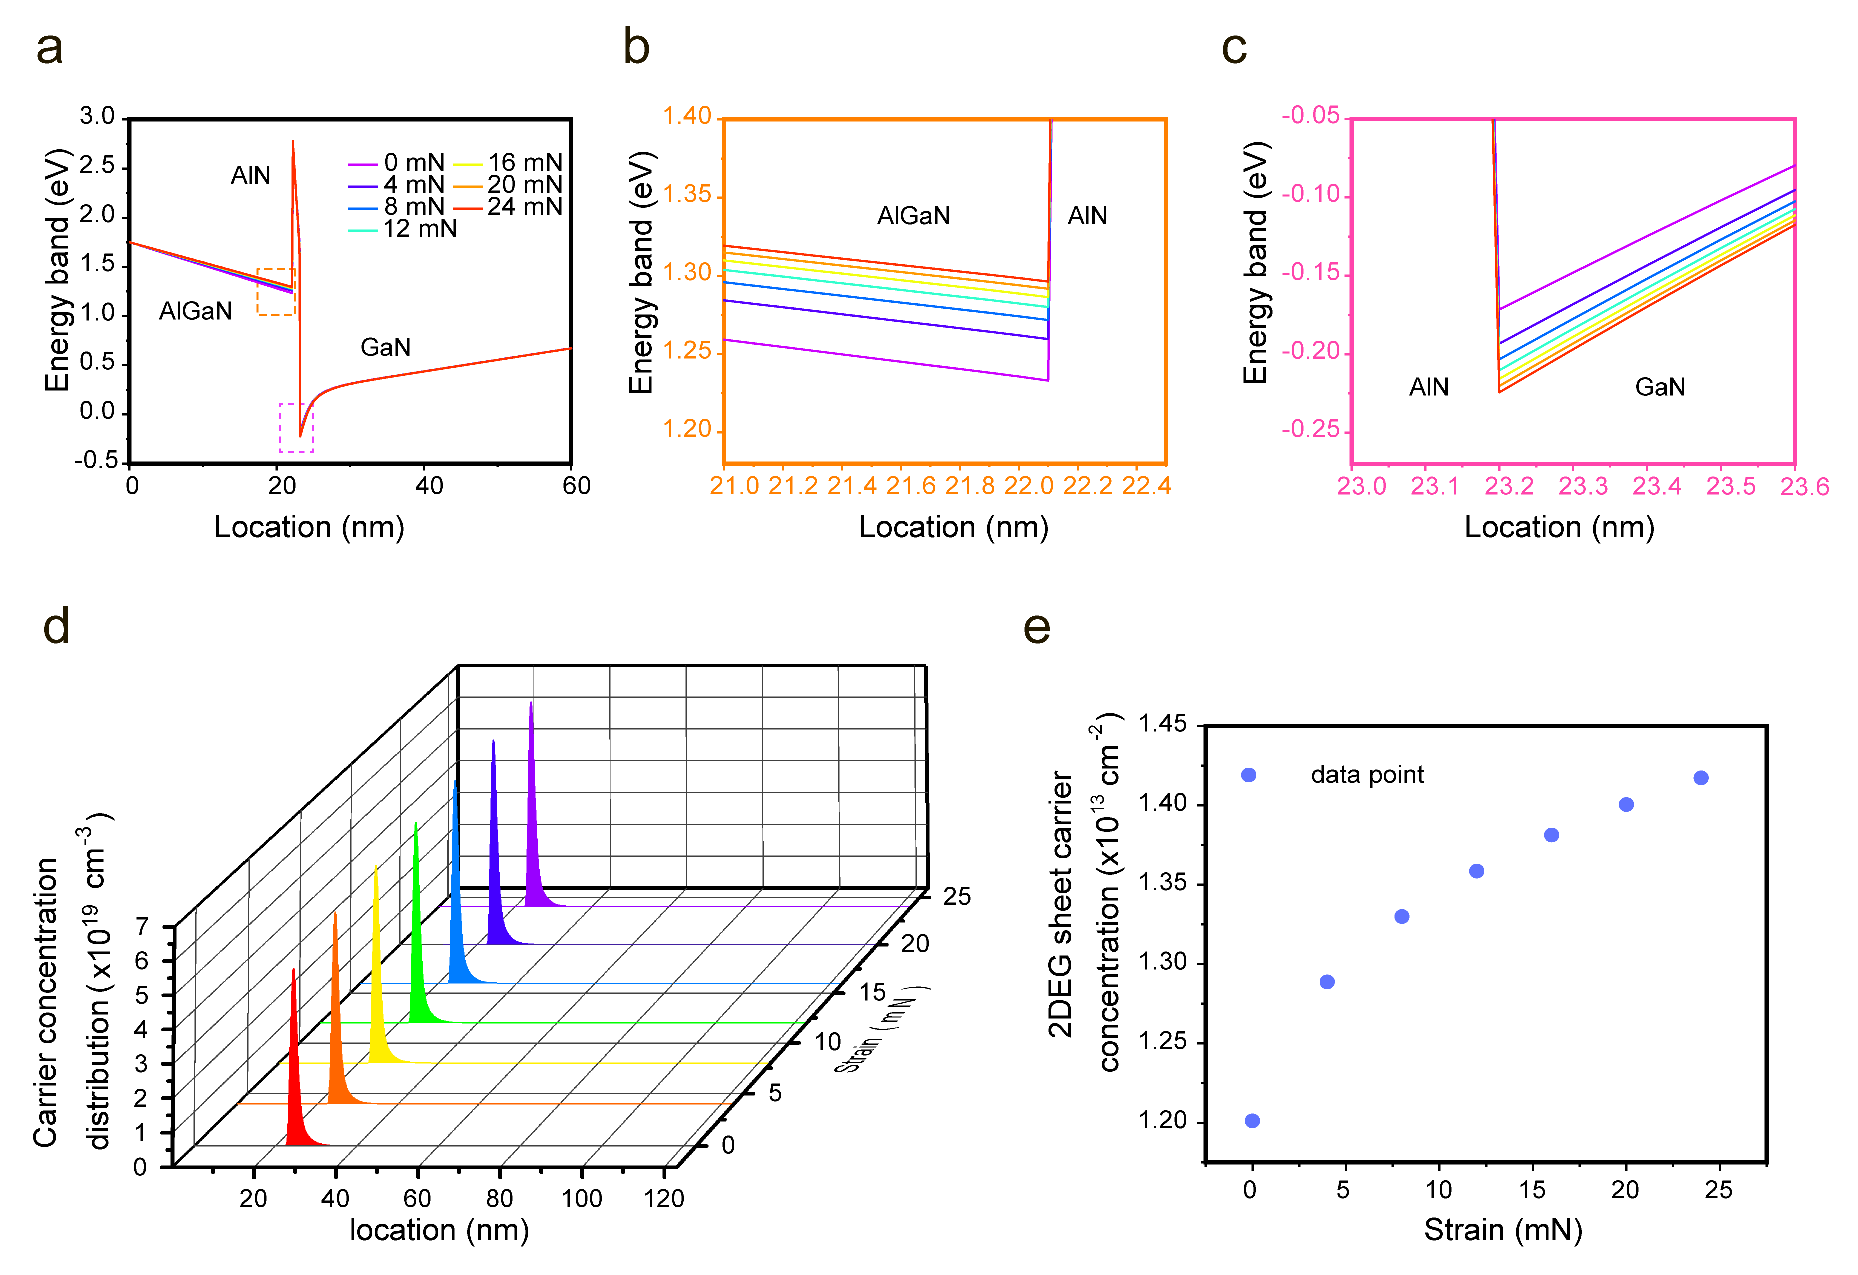
\includegraphics[width=0.9\textwidth]{ch2_400}
\caption[Simulation results of MEMS with the cantilever length of 400 \unit{\um} under downward force]{Simulation results of MEMS with the cantilever length of 400 \unit{\um} under downward force}
\label{fig:2.400}
\end{figure}

\begin{figure}[H] 
\centering    
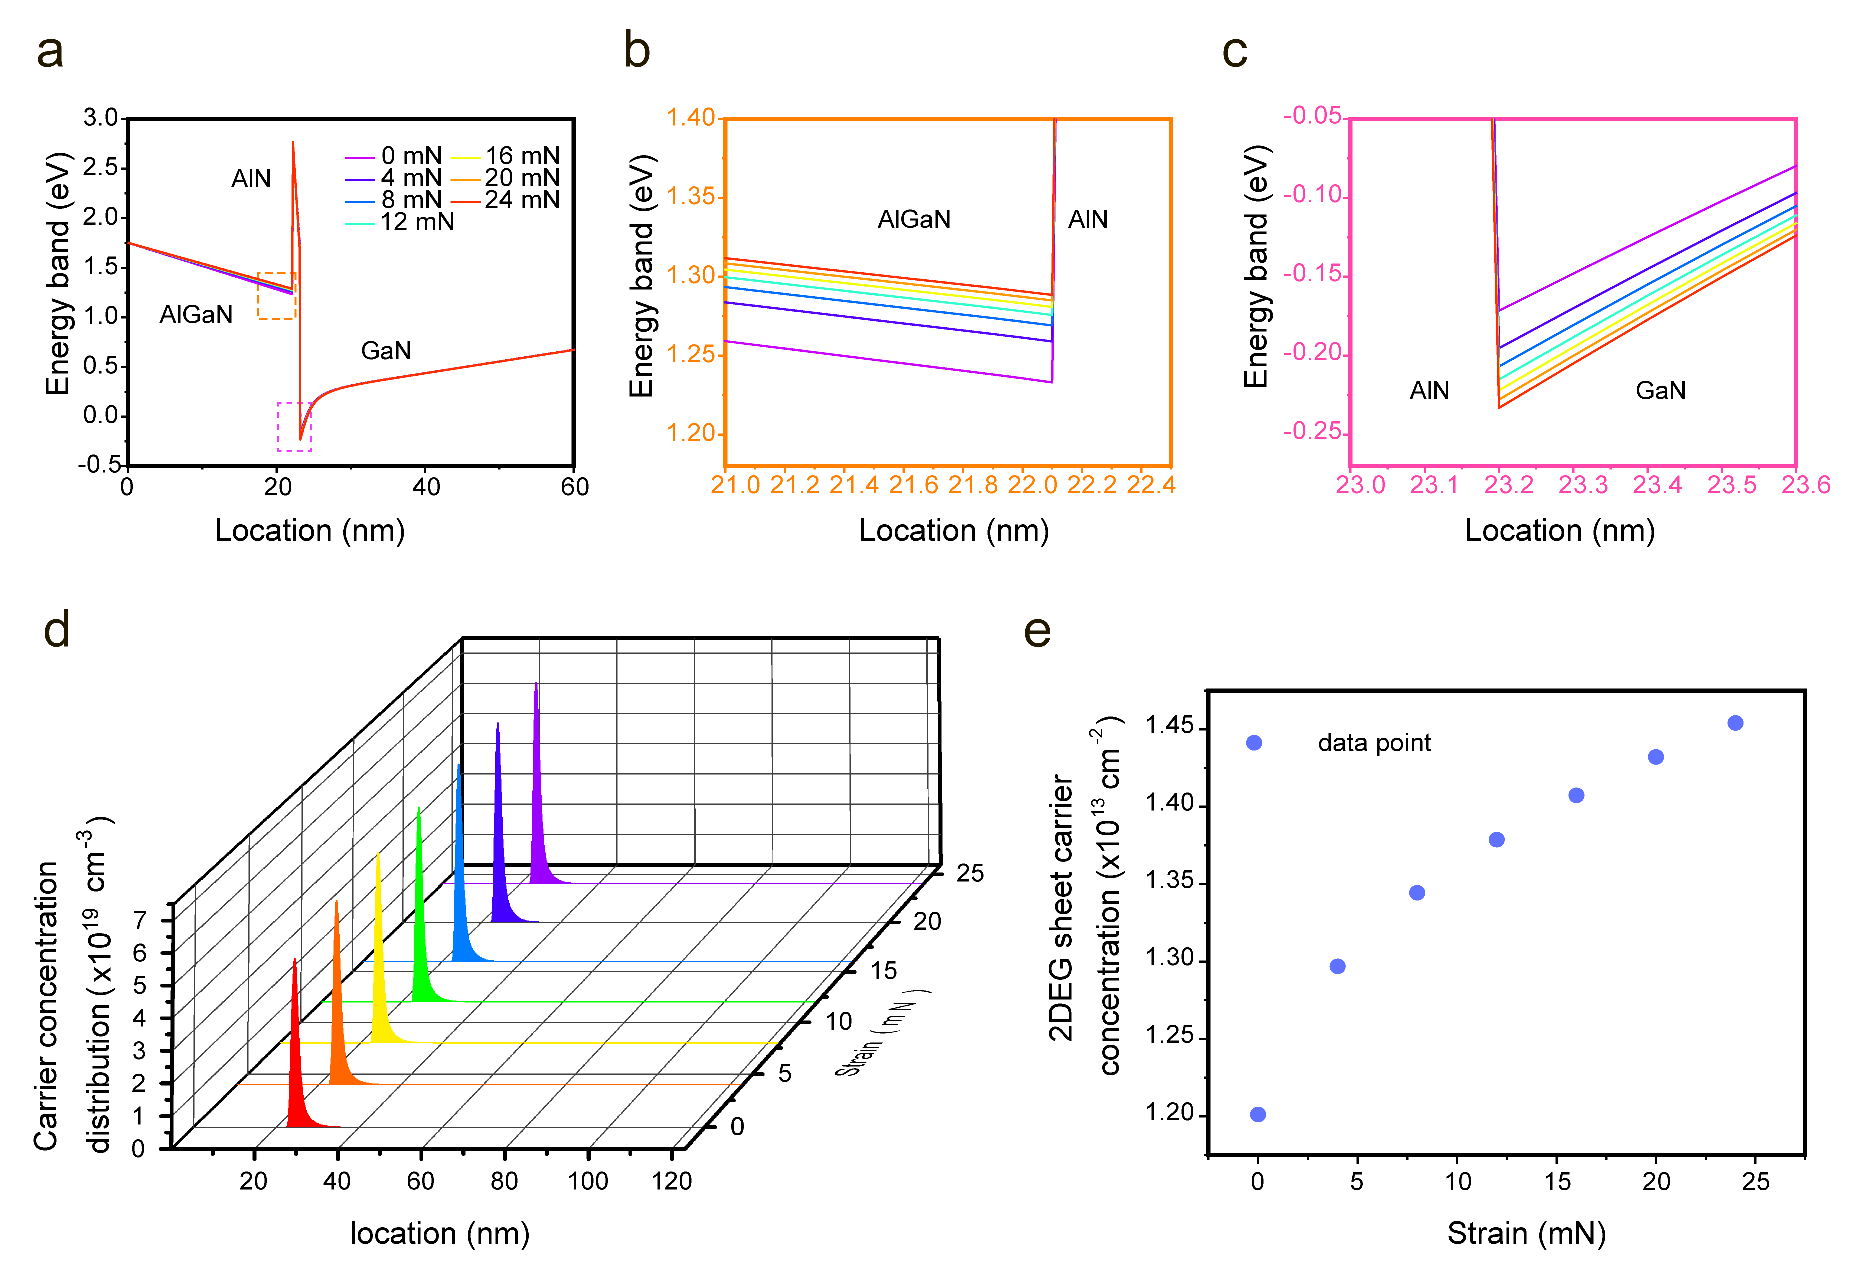
\includegraphics[width=0.85\textwidth]{ch2_450}
\caption[Simulation results of MEMS with the cantilever length of 450 \unit{\um} under downward force]{Simulation results of MEMS with the cantilever \index{Cantilever} length of 450 \unit{\um} under downward force}
\label{fig:2.450}
\end{figure}

\begin{figure}[H] 
\centering    
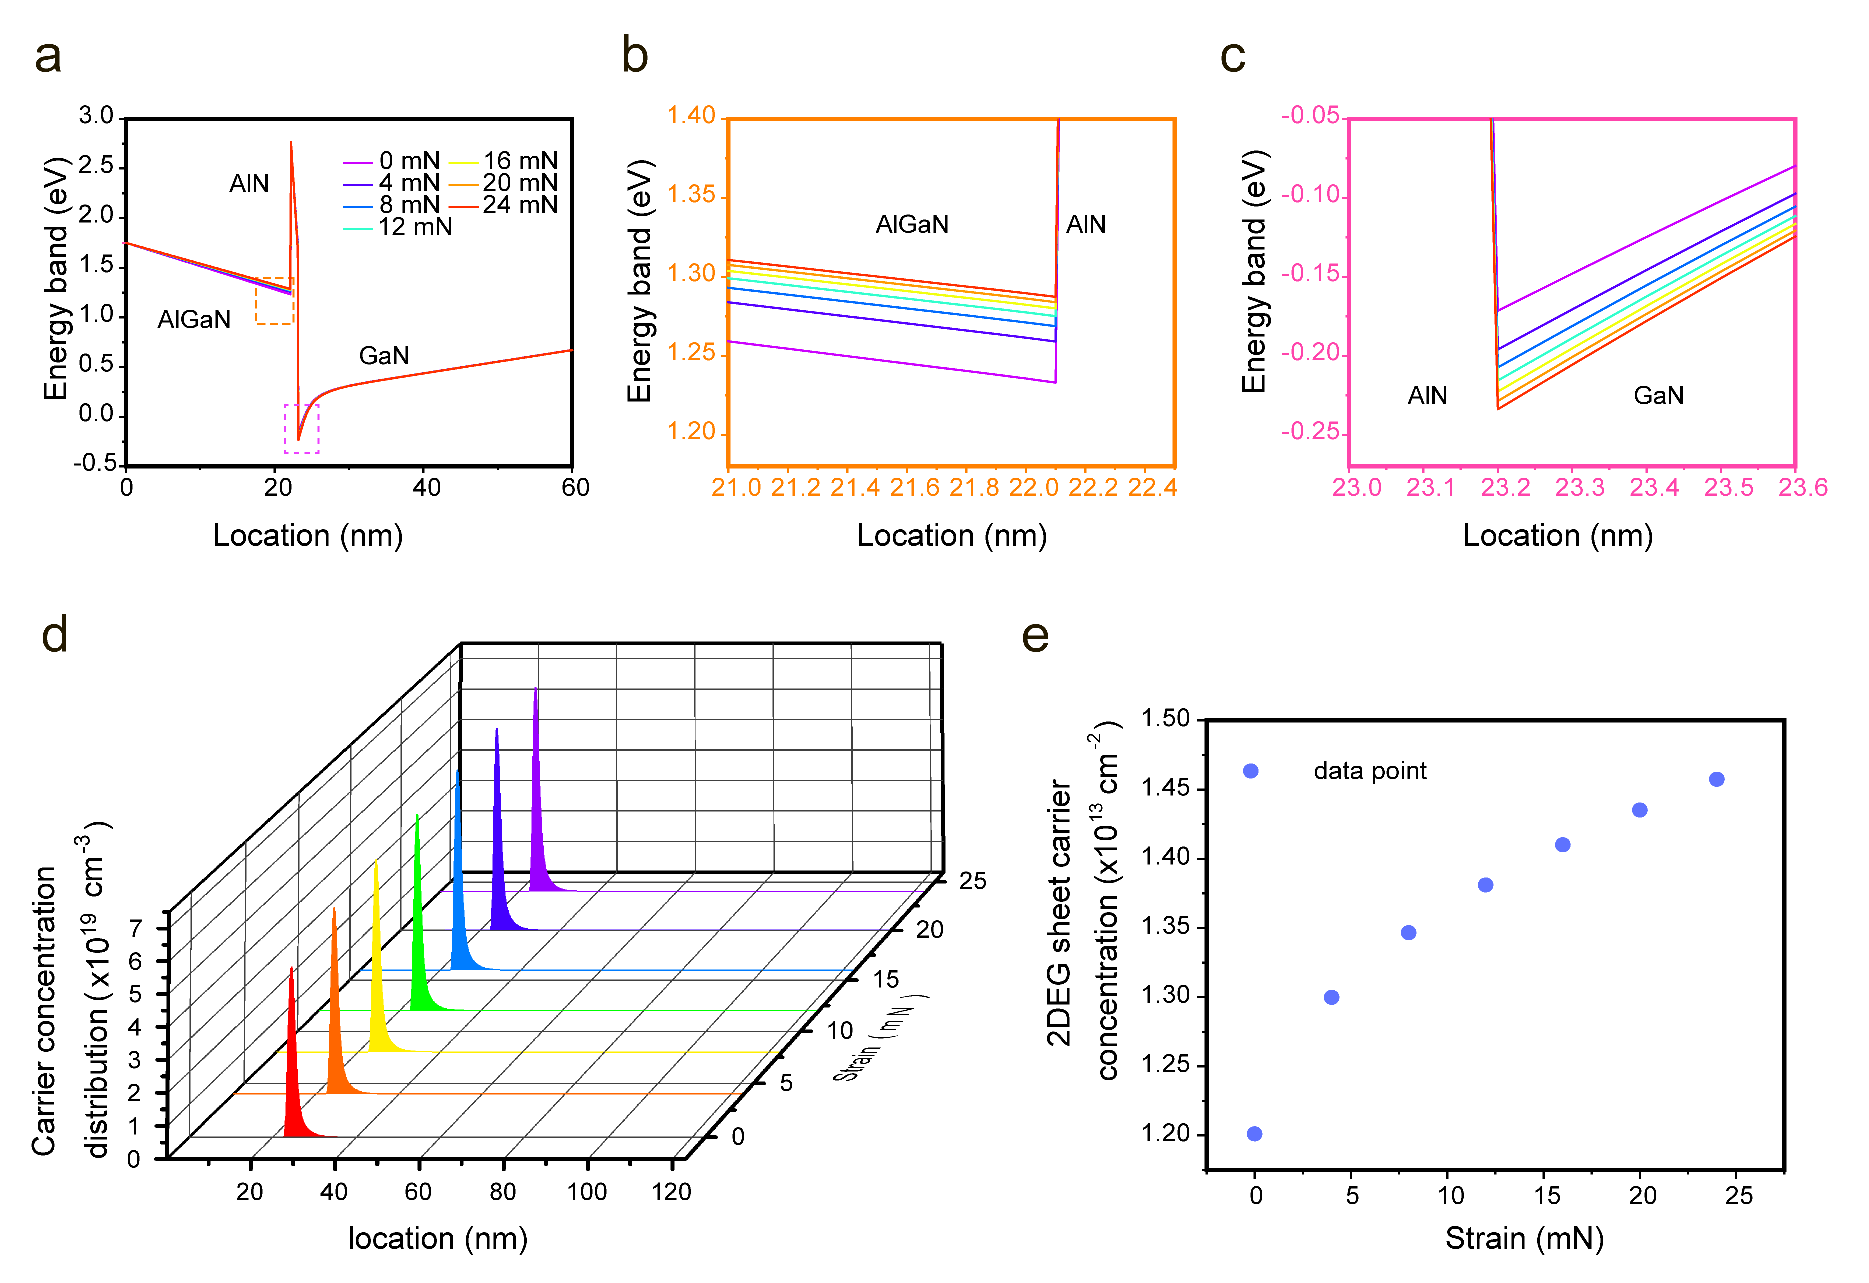
\includegraphics[width=0.85\textwidth]{ch2_500}
\caption[Simulation results of MEMS with the cantilever length of 500 \unit{\um} under downward force]{Simulation results of MEMS with the cantilever length of 500 \unit{\um} under downward force}
\label{fig:2.500}
\end{figure}

\section{Summary}
In this study, a semi-classical physical model of the MEMS \index{MEMS} device with a cantilever \index{Cantilever} structure based on AlGaN/AlN/GaN heterojunction was established by using piezoelectric theory. The mathematical relationship between the lattice strain \index{Lattice!strain} and the piezoelectric polarization charge \index{Piezoelectric!polarization charge} of the multilayer heterojunction film was deduced through piezoelectric constitutive equation \index{Piezoelectric!constitutive equation} and \index{Biaxial stress model} biaxial stress model. Then the finite element analysis \index{Finite element analysis} method of material mechanics was used to calculate the piezoelectric polarization charge intensity \index{Piezoelectric!polarization charge} of the heterojunction film under different external stresses, and the one-dimensional Schrödinger-Poisson self-consistent coupling model was used to calculate the modulation \index{Modulation} characteristics of the external stress on the energy band of the AlGaN/AlN/GaN heterojunction \index{AlGaN/AlN/GaN heterojunction} and the electrical properties of the \index{MEMS} MEMS device. The theoretical results successfully verify the experimental results of the new MEMS devices designed and fabricated in this paper, namely SPD and MPD. The model provides theoretical guidance for the development of novel MEMS cantilever \index{Cantilever} devices based on \index{AlGaN/AlN/GaN heterojunction} AlGaN/AlN/GaN heterojunctions.

\nomenclature{$P_{PE}$}{Piezoelectric polarization charge density}
\nomenclature{$P_{Psp}$}{Spontaneous polarization charge density}
\nomenclature{$P_{GaN}^{PE}$}{Piezoelectric polarization charge density of GaN}
\nomenclature{$P_{AlGaN}^{PE}$}{Piezoelectric polarization charge density of AlGaN}
\nomenclature{$P_{AlN}^{PE}$}{Piezoelectric polarization charge density of AlN}
\nomenclature{$P_{GaN}^{sp}$}{Spontaneous polarization charge density of GaN}
\nomenclature{$P_{AlN}^{sp}$}{Spontaneous polarization charge density of AlN}
\nomenclature{$P_{AlGaN}^{sp}$}{Spontaneous polarization charge density of AlGaN}
\nomenclature{$Al_{x}Ga_{1-x}N$}{The percentage of AlN in AlGaN}
\nomenclature{$b_{A l_{x} G a_{1-x} N}$}{Bending coefficient of AlGaN}
\nomenclature{$e_{ijk}$}{Nonlinear piezoelectric coefficient of GaN crystal}
\nomenclature{$S_{\perp}$}{Lattice strains perpendicular to c-plane of GaN crystal}
\nomenclature{$S_{\|}$}{Lattice strains parallel to c-plane of GaN crystal}
\nomenclature{$k_{B}$}{Boltzmann constant}
\nomenclature{$T$}{Electron temperature}
\nomenclature{$N_{e}$}{Sum of the electron densities in all the subbands}
\nomenclature{$\boldsymbol{E}$}{Electric field strength vector}
\nomenclature{$\boldsymbol{D}$}{Electric displacement vector}
\nomenclature{$\sigma$}{Stress tensor}
\nomenclature{$\boldsymbol{c}_{E}$}{Elastic coefficient tensor}
\nomenclature{$\boldsymbol{e}$}{Linear piezoelectric coefficient}
\nomenclature{$\boldsymbol{k}$}{Dielectric constant tensor}
\nomenclature{$\boldsymbol{S}$}{Strain tensor}
\nomenclature{$P_{interface}$}{The density of polarization charges at the interface}
\nomenclature{$n_{i}$}{Density of electrons in the ith subband}
\nomenclature{$S_{x x}, S_{x}$}{Strains in the $x$ direction}
\nomenclature{$S_{y y}, S_{y}$}{Strains in the $y$ direction}
\nomenclature{$S_{z z}, S_{z}$}{Strains in the $z$ direction}
\nomenclature{$\varepsilon_{0}$}{Vacuum permittivity}
\nomenclature{$\mathbf{P}$}{Electric polarization strength}
\nomenclature{$P_{z}$}{Piezoelectric polarization in the $z$ direction}
\nomenclature{$v$}{Poisson's ratio}

\nomenclature{$a_{AlGaN}$}{Lattice constant of AlGaN}
\nomenclature{$a_{AlN}$}{Lattice constant of AlN}
\nomenclature{$a_{GaN}$}{Lattice constant of GaN}


\nomenclature{$N_{D}^{+}$}{Donor ion concentration}
\nomenclature{$n(x)$}{Concentrations of free electrons}
\nomenclature{$p(x)$}{Concentrations of holes}

\nomenclature{$\varepsilon(x)$}{Dielectric constant AlGaN, AlN and GaN}
\nomenclature{$N_{A}^{-}$}{Acceptor ion concentration}
\nomenclature{$q$}{Absolute value of the unit charge}

\nomenclature{$V_{c}(x)$}{Conduction band edge potential}
\nomenclature{$V_{h}(x)$}{Hartree potential}
\nomenclature{$V_{x c}(x)$}{Exchange-correlated potential}

\nomenclature{$S_{B}$}{Stain of the thin film $B$}

\nomenclature{$a_{A}$}{Lattice constant of the substrate $A$}
\nomenclature{$a_{B}(epi)$}{Lattice constant of the thin film $B$}
\nomenclature{$a_{AlN}(strain)$}{Lattice constant of strained AlN}
\nomenclature{$a_{GaN}(strain)$}{Lattice constant of strained GaN}
\nomenclature{$a_{AlGaN}(strain)$}{Lattice constant of strained AlGaN}
\nomenclature{$S_{AlN}(strain)$}{Strain of strained AlN}
\nomenclature{$S_{GaN}(strain)$}{Strain of strained GaN}
\nomenclature{$S_{AlGaN}(strain)$}{Strain of strained AlGaN}
\nomenclature{$a$}{Lattice constant}
\nomenclature{$c$}{Lattice constant}
\nomenclature{$E_{g}$}{Bandgap energy}
\nomenclature{$e31$}{Piezoelectric Constant}
\nomenclature{$e33$}{Piezoelectric Constant}
\nomenclature{$e311$}{Piezoelectric Constant}
\nomenclature{$e333$}{Piezoelectric Constant}
\nomenclature{$e133$}{Piezoelectric Constant}
\nomenclature{$C11$}{Elastic constants}
\nomenclature{$C12$}{Elastic constants}
\nomenclature{$C13$}{Elastic constants}
\nomenclature{$C33$}{Elastic constants}

\nomenclature{$𝑆_{xx}(GaN)$}{Strain of GaN in the $x$ direction}
\nomenclature{$𝑆_{yy}(GaN)$}{Strain of GaN in the $y$ direction}
\nomenclature{$𝑆_{zz}(GaN)$}{Strain of GaN in the $z$ direction}
\nomenclature{$m^{*}$}{Effective mass of the electron}
\nomenclature{$V(x)$}{Potential energy}
\nomenclature{$E_{i}$}{Energy of the ith subband}
\nomenclature{$\psi_{i}(x)$}{Wave function of the ith subband}


\nomenclature[z-GaN]{GaN}{Gallium nitride}
\nomenclature[z-AlN]{AlN}{Aluminum nitride}
\nomenclature[z-AlGaN]{AlGaN}{Aluminium gallium nitride}
\nomenclature[z-AlN]{HEMT}{High-electron-mobility transistor}
\nomenclature[z-2DEG]{2DEG}{The two-dimensional electron gas}
\nomenclature[z-AlN]{FET}{Field effect transistor}
\part{Manufacturing}

% **************************** Define Graphics Path **************************



%!TEX root = ../thesis.tex
%*******************************************************************************
%****************************** Third Chapter **********************************
%*******************************************************************************
\chapter{Manufacturing Technology of Power MEMS Devices}
\label{ch:Manufacturing Technology of Power MEMS Devices}

% **************************** Define Graphics Path **************************
\ifpdf
    \graphicspath{{Chapter6/Figs/Raster/}{Chapter6/Figs/PDF/}{Chapter6/Figs/}}
\else
    \graphicspath{{Chapter6/Figs/Vector/}{Chapter6/Figs/}}
\fi

In the Part II, I would systematically study the manufacture of GaN power MEMS devices from epitaxial growth \index{Epitaxial!growth} wafers \index{Wafer} to well-functional devices. Benefiting from the rapid development of III-V compound semiconductor fabrication and characterization equipment, various complex microstructures including GaN microcantilever \index{Cantilever} structures can now be easily realized by equipment devices with different functions. This chapter will introduce the main nanofabrication and characterization equipment, including epitaxial growth, dry \index{Etching!dry etching} etching, photolithography, thin \index{Photolithography} film \index{Thin film} deposition, plasma \index{Cleaning!plasma cleaning} cleaning, Raman \index{Raman!spectroscopy} spectroscopy, scanning electron \index{Scanning electron microscopy (SEM)} microscopy, transmission \index{Transmission electron microscopy (TEM)} electron microscopy, etc. I would briefly introduce their important role in GaN power MEMS \index{MEMS} research, as well as the corresponding process \index{Fabrication process} design and key parameters. The equipment mentioned in this chapter and later all belong to the micro-nano processing platform of the Chinese Academy of Sciences. The pictures of some of the equipment are from the official website of the equipment manufacturer, and all the models shown here are in one-to-one correspondence with the real objects.

\section{Fabrication techniques}

\subsection{GaN-on-Si wafer epitaxial growth}

\begin{figure}[H] 
\centering    
\includegraphics[width=0.8\textwidth]{MOCVD}
\caption[Aixtron CCS 3×2 MOCVD]{Aixtron CCS 3×2 MOCVD}
\label{fig:MOCVD}
\end{figure}

The GaN wafers \index{Wafer} are typically obtained by epitaxial growth \index{Epitaxial!growth} on Si substrates \index{Substrate} due to the less \index{Lattice!mismatch} lattice mismatch. Metal \index{MOCVD} Organic Compound Chemical Vapor Deposition (MOCVD), also known as Metal Organic Vapor Phase Epitaxy (MOVFE) is an important method for preparing nitride \index{Nitride} semiconductor materials, and it is also the most widely used method in the industry. MOCVD uses organic compounds of group III and group II elements and hydrides of group V and group VI elements as crystal \index{Crystal} growth source materials, and conducts vapor phase epitaxy on the Si substrate by thermal decomposition reaction to grow various III-V group, II-VI group compound semiconductors and their multicomponent solid solutions.

The growth of nitride crystals \index{Crystal} is usually carried out in cold-wall or hot-wall reaction chambers under normal or low pressure (\num{1e1} $\sim$ \num{1e5} \unit{\Pa}). In the \index{Epitaxial!growth} growth of GaN materials, trimethylgallium (\ce{TMG}) and ammonia gas (\ce{NH3}) carried by \ce{H2} are usually injected into the reaction chamber at the same time, and the reaction gases are transported to the surface of the high-temperature substrate \index{Substrate} and mixed above. The chemical reaction occurs as follows:
\begin{equation}
\mathrm{Ga}\left(\mathrm{CH}_{3}\right)_{3} \text { (gas) }+\mathrm{NH}_{3} \text { (gas) } \rightarrow \mathrm{GaN} \text { (solid) }+3 \mathrm{CH}_{4} \text { (gas) }
\end{equation}
the resulting GaN molecules are deposited on the surface of the Si substrate to form an epitaxial film \cite{hao2016nitride}.

\begin{figure}[H] 
\centering    
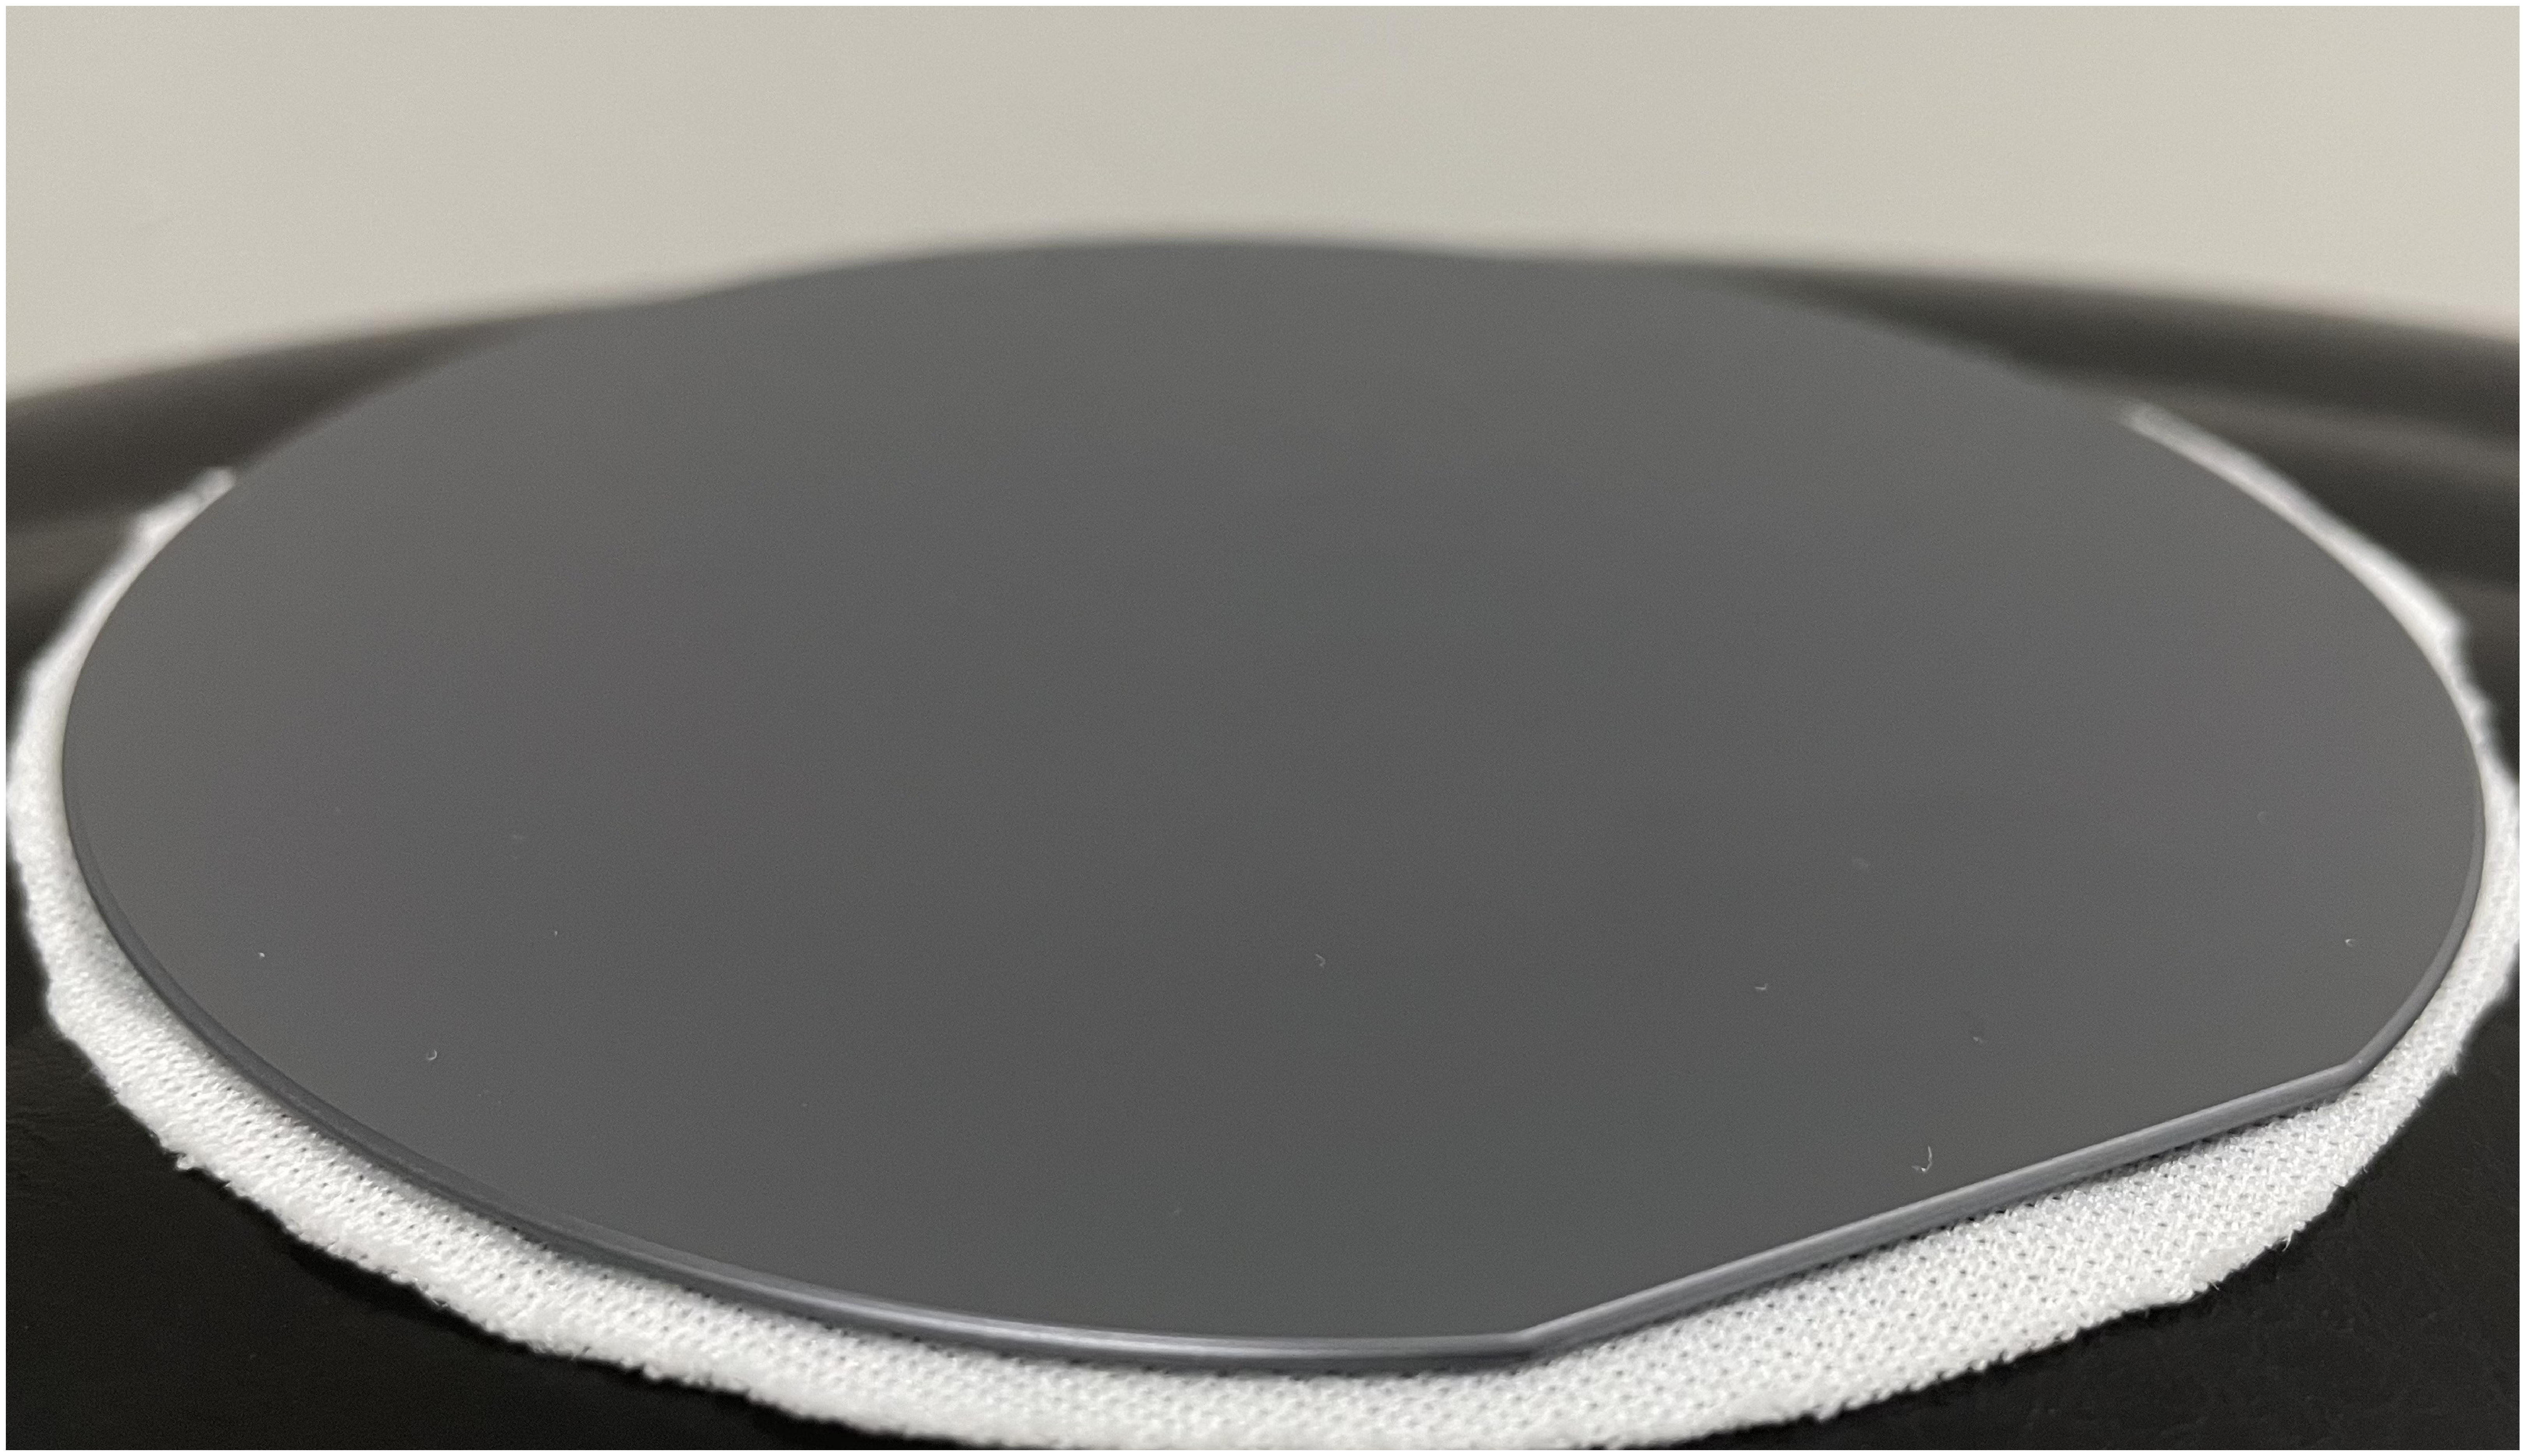
\includegraphics[width=0.7\textwidth]{wafer}
\caption[The 3-inch GaN-on-Si wafer]{The 3-inch GaN-on-Si wafer}
\label{fig:wafer}
\end{figure}

In this research, the 3-inch GaN-on-Si wafers \index{Wafer} have been successfully epitaxially grown on Si(111) substrates \index{Substrate} using Aixtron CCS 3×2 MOCVD, as shown in \autoref{fig:wafer}. The total thickness is about 1 \unit{\mm}, including Si(111) substrate, AlN/AlGaN multi-layer buffer layer, unintentionally doped (UID) GaN buffer layer, intrinsic GaN \index{Two-dimensional electron gas (2DEG)} 2DEG channel \index{Channel} layer, AlN barrier layer, AlGaN barrier layer and GaN cap layer. The grown wafer exhibits good electrical performance with 300 \unit{\ohm}/square sheet resistance, \num{1.00e13} \unit{\per\square\cm} carrier density, 2000 \unit{\square\cm/(Vs)} mobility \index{Electron mobility} and \SI{600}{\volt} breakdown \index{Voltage!breakdown voltage} voltage.

\subsection{Wafer dicing}

\begin{figure}[H] 
\centering    
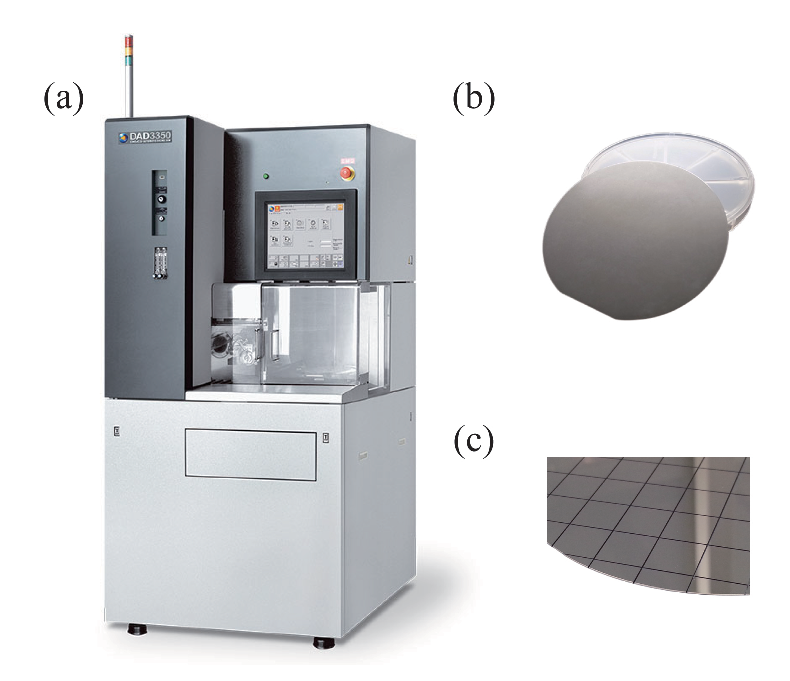
\includegraphics[width=0.8\textwidth]{CUT}
\caption[DISCO DAD3350 automatic dicing saw]{DISCO DAD3350 automatic dicing saw}
\label{fig:CUT}
\end{figure}

Compound semiconductors, such as GaN and SiC, are difficult to obtain high productivity with slow feed rates when using existing diamond blades for blade cutting, especially as wafer thickness becomes thinner. Therefore, utilizing beneficial characteristics of laser energy, laser cutting has developed as a highly promising method in dicing-grinding \index{Dice} service. Laser applications minimize kerf streets, thereby suiting special materials such as GaN or SiC when blade dicing reaches its limits. Further, working with laser technology provides a high degree of flexibility to die forms while offering high processing speed. Laser technology is developing rapidly and the semiconductor industry is taking full advantage of every innovation leap.

In this research, dice of size \numproduct{2 x 2} \unit{\mm} and \numproduct{3 x 3} \unit{\mm} have been cut from the grown 3-inch wafers \index{Wafer} with the DISCO DAD3350 automatic dicing saw.

\subsection{Cleaning technologies}
Cleaning procedures are essential steps in semiconductor processing. These are mostly used to remove particles and oxidize organic contaminants. Just a single particle on a \index{Wafer} wafer is enough to cause a killer defect or excursion that will ultimately lead to device failure. This is because both device reliability and final product yields are directly linked to the cleanliness of a wafer as it passes through the hundreds of patterning, etching, deposition and interconnect process steps. Therefore, the wafer must be strictly cleaned to remove organic and inorganic substances on the surface before the device fabrication process. The precondition of the cleaning process is not to destroy the surface characteristics of the epitaxial wafer. On this basis, the cleaning technologies, including wet cleaning and \index{Cleaning!dry cleaning} dry cleaning, are used to effectively remove various residual contaminants and impurities on the surface of the epitaxial \index{Surface} wafer. 

\begin{description}
	
\item [Wet cleaning] Some \index{Cleaning!wet cleaning} common cleaning solvents include acetone, trichloroethylene, ultrapure water, hydrochloric \index{Hydrochloric acid} acid, piranha solution, dilute HF \index{Hydrofluoric acid} solution and RCA cleaner. The cleaning steps of acetone, trichloroethylene, ultrapure water and hydrochloric acid are simple and will not be repeated. Piranha solution, dilute HF solution, and RCA cleaner are described as follows because of their better cleaning effect and certain dangers during the operation \cite{reinhardt2018handbook,king1998cleaning,tsujiwet}.

\begin{itemize}
\item[1.] Piranha solution

It consists of \ce{H2SO4} (98$\%$) and \ce{H2O2} (30$\%$) in different ratios, and is typically used for removing organic contaminants \index{Piranha solution} and \index{Photoresist} stripping photoresists.


\item[2.] RCA clean

The RCA clean \index{Wafer} is a \index{Cleaning!RCA cleaning} standard set of wafer cleaning steps which need to be performed before high-temperature processing steps (oxidation, diffusion, CVD) of wafers in semiconductor manufacturing. It involves the following chemical processes performed in sequence:

\begin{itemize}
	\item[2.1)] SC-1: organic clean + particle clean
	
	5 parts of deionized \index{Deionized water} water, 1 part of ammonia water, (29$\%$ by weight of \ce{NH3}), and 1 part of \index{Hydrogen peroxide} aqueous \ce{H2O2} (hydrogen peroxide, 30$\%$) at \SI{75}{\degreeCelsius} or \SI{80}{\degreeCelsius} typically for 10 minutes. This base-peroxide mixture removes organic residues. Particles are also very effectively removed, even insoluble particles. 
    
    \item[2.2)] SC-2: ionic clean
	
	6 parts of deionized water, 1 part of aqueous \index{Hydrochloric acid} HCl (hydrochloric acid, 37$\%$ by weight), and 1 part of aqueous \ce{H2O2} (hydrogen peroxide, 30$\%$)
at 75 or \SI{80}{\degreeCelsius} typically for 10 minutes. This treatment effectively removes the remaining traces of metallic (ionic) contaminants.
\end{itemize}

\item[3.] Dilute HF solution

Prepared by diluting 49$\%$ HF \index{Hydrofluoric acid} with dionized water (1:100) at room temperature and can effectively removes the oxide.

\end{itemize}

In this research, wet \index{Cleaning!wet cleaning} cleaning techniques have been applied to wafer \index{Wafer} cleaning, residual photoresist \index{Photoresist} removal, silicone oil cleaning, organic and particle contamination removal.


\begin{figure}[t] 
\centering    
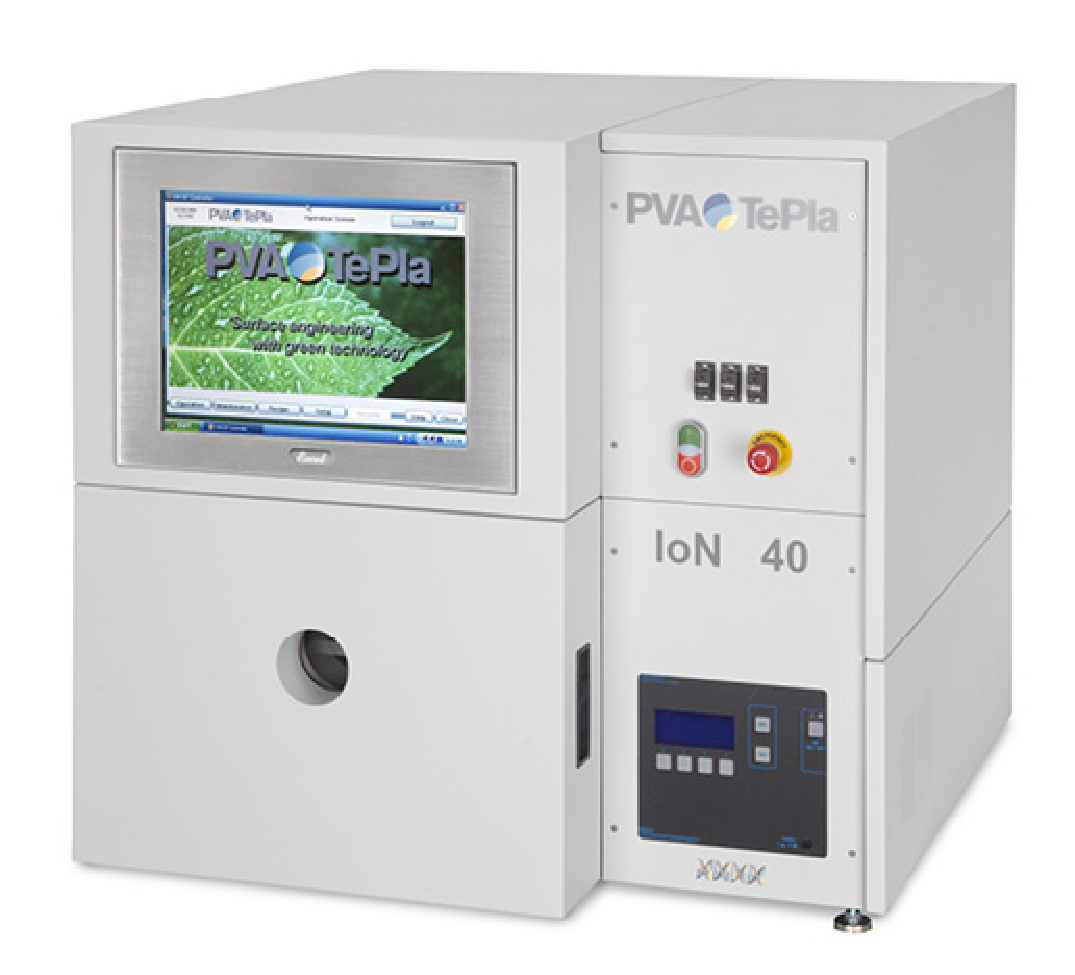
\includegraphics[width=0.6\textwidth]{plasma}
\caption[PVA TePla IoN 40 plasma cleaner]{PVA TePla IoN 40 plasma cleaner}
\label{fig:plasma}
\end{figure}

\item [Dry cleaning] Plasma technology is often characterized as a "dry" cleaning \index{Cleaning!dry cleaning} process, using ionized gases in vacuum chambers to remove all organic matter from the surface of the semiconductors through the use of an ionized gas called plasma. Plasma is an ionized gas capable of conducting electricity and absorbing energy from an electrical supply. Manmade plasma is generally created in a low-pressure environment. When a gas absorbs electrical energy, its temperature increases causing the ions to vibrate faster and "scrub" a \index{Surface} surface. This is generally performed in a vacuum chamber utilizing oxygen and/or argon gas and is an effective way to clean without using hazardous solvents. In contrast to chemically-based wet technologies, which have their role in removing thicker contaminants in the \index{Cleaning!plasma cleaning} micron range, plasma deals with contamination in the nanometer range on substrate and wafer surfaces.

In this research, PVA TePla IoN 40 plasma cleaner is mainly used to remove residual photoresist \index{Photoresist} and organic cleaning solutions by generating oxygen ions.
 
\end{description}

Cleaning technologies are crucial steps in the semiconductor manufacturing process and directly affects the performance and reliability of the device. In the process integration of \autoref{ch:Process Development and Integration of Power MEMS Devices}, a large number of cleaning processes can be found between lithography, etching, deposition, etc. They connect all processes as an indispensable intermediate link. The purpose of the cleaning process is to remove the residual influence of the previous process to the greatest extent on the premise of retaining the previous process results, and to provide a good operating environment for the subsequent process.

\subsection{Photolithography}

\begin{figure}[H] 
\centering    
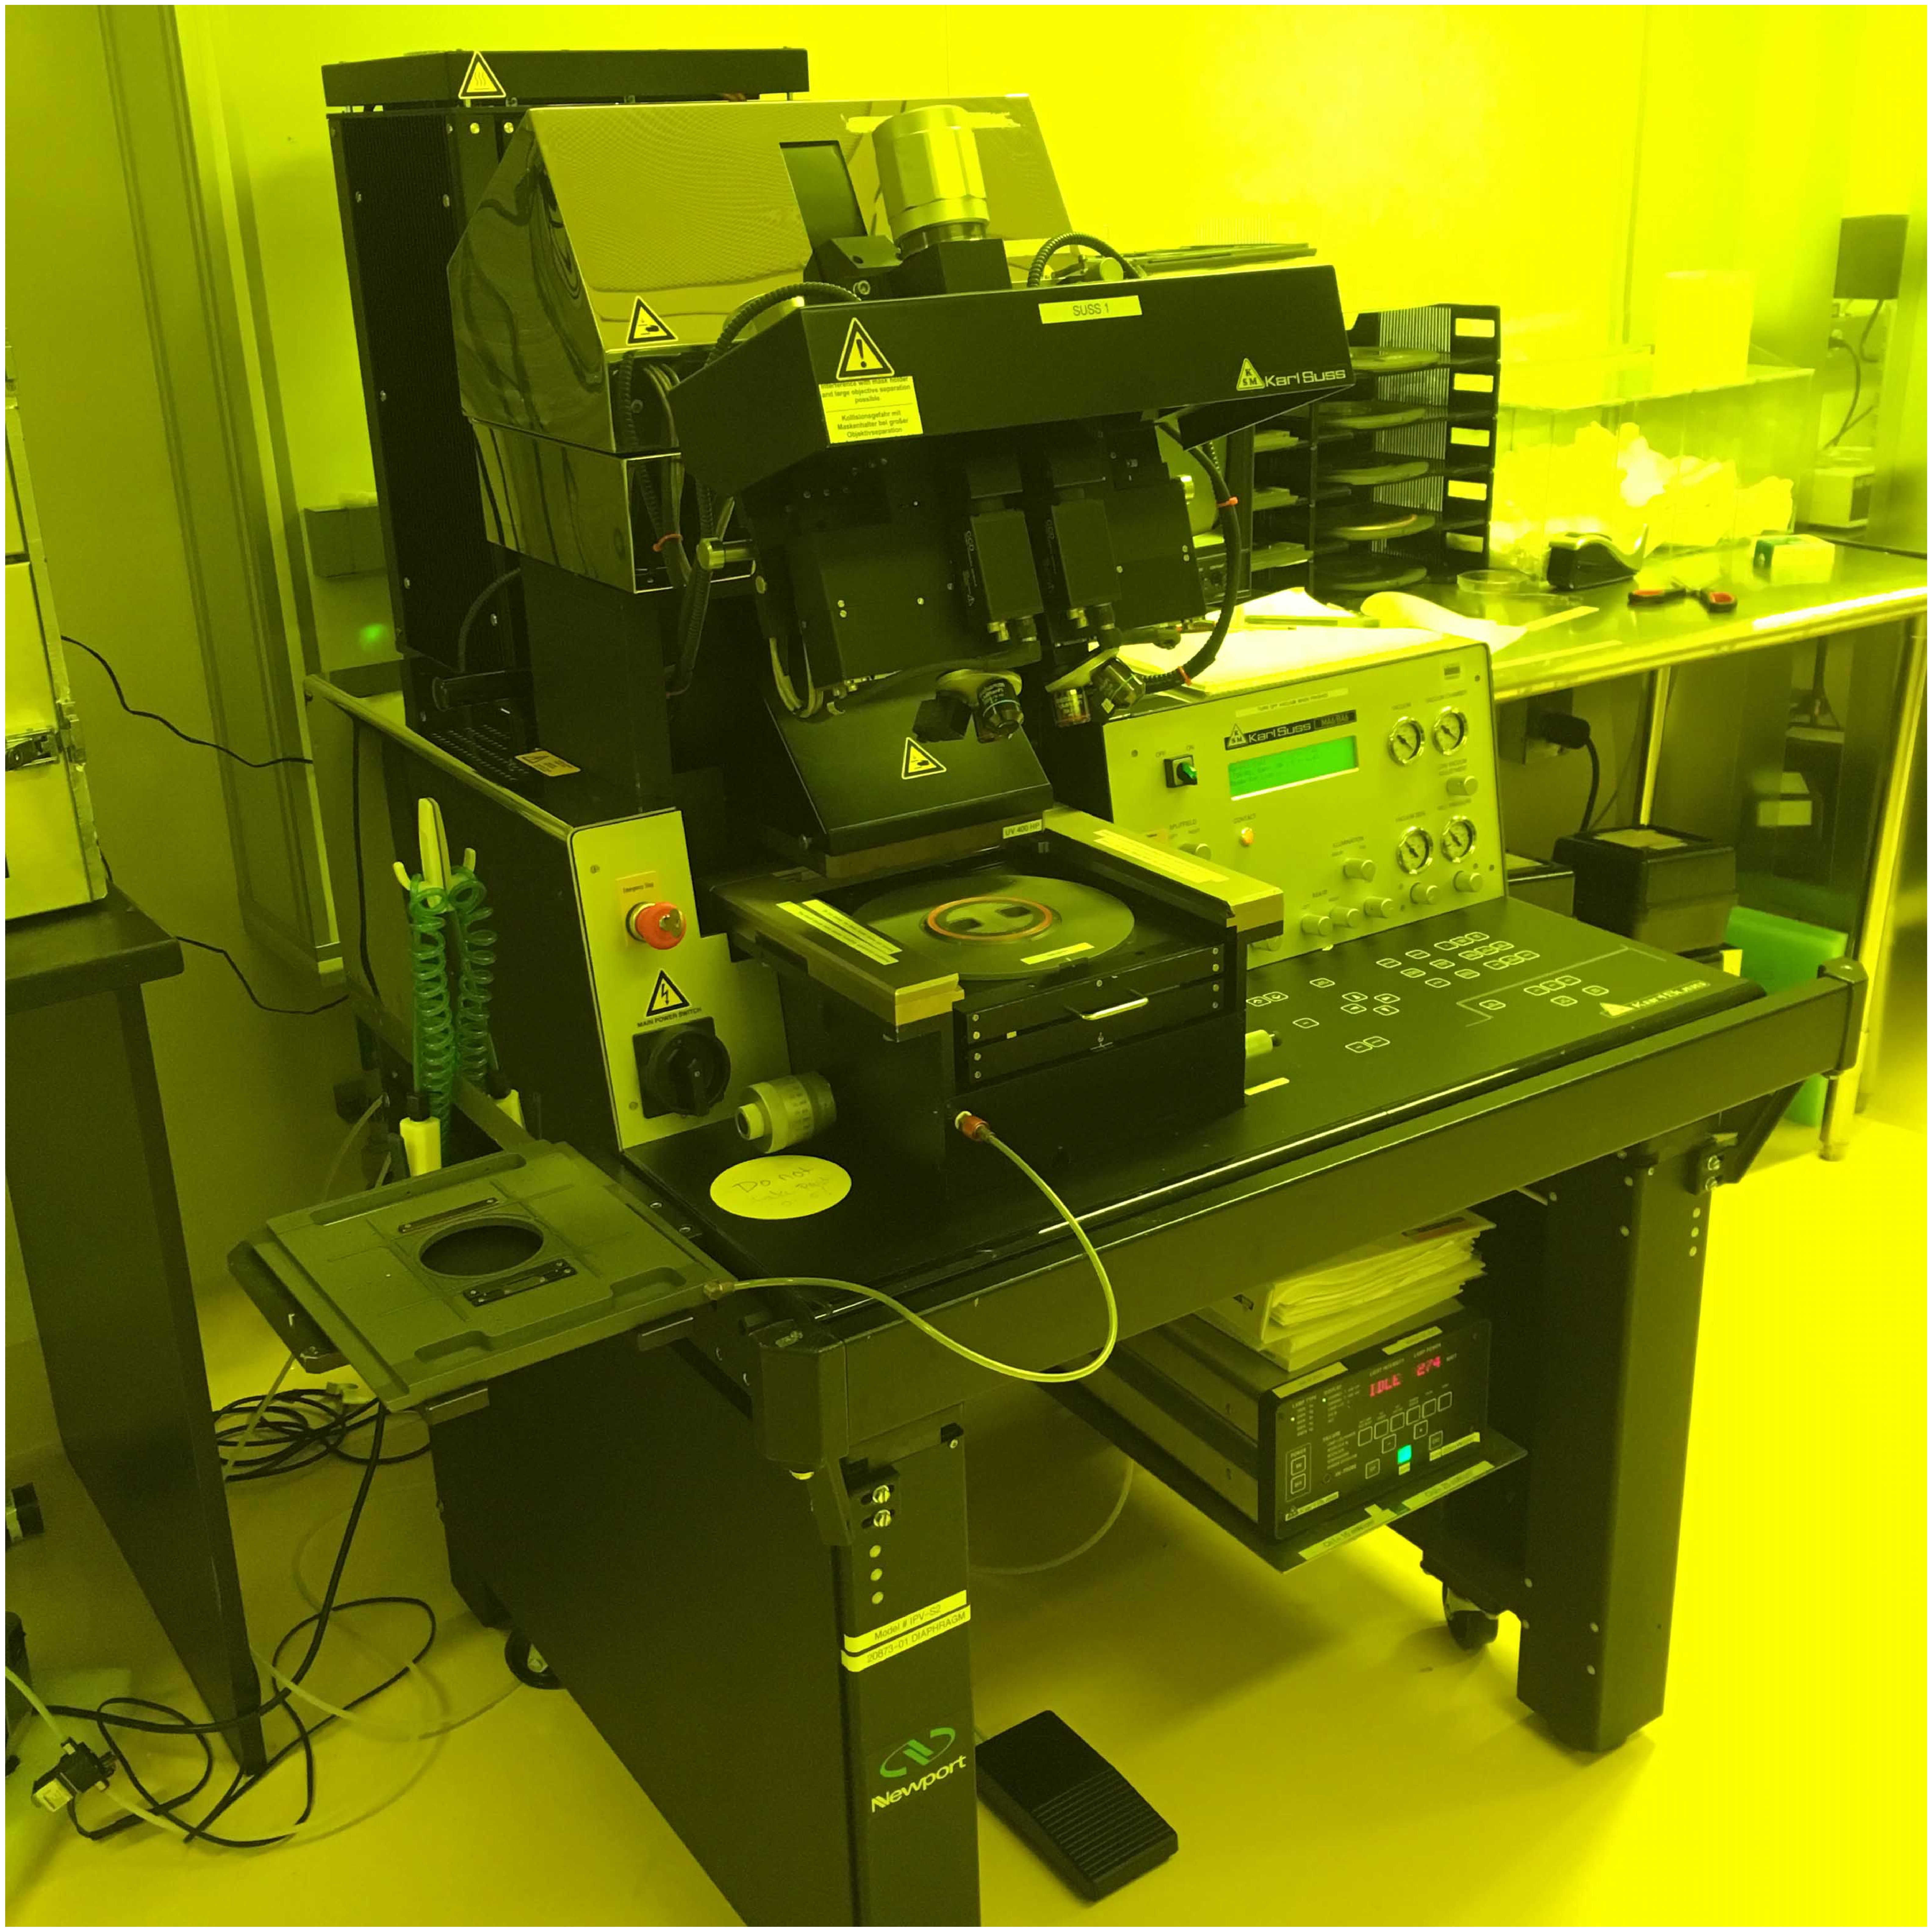
\includegraphics[width=0.6\textwidth]{photolithography}
\caption[SUSS MA6 mask aligner designed for high-resolution photolithography]{SUSS MA6 mask aligner designed for high-resolution photolithography}
\label{fig:photolithography}
\end{figure}

Photolithography \index{Photolithography} is an optical means of transferring a pattern on a \index{Substrate} substrate. It uses light to produce minutely patterned \index{Thin film} thin films of suitable materials over a substrate to protect selected areas of it during subsequent etching, deposition, or implantation operations. Typically, ultraviolet light is used to transfer a geometric design from an optical mask to a light-sensitive chemical \index{Photoresist} (photoresist) coated on the substrate. The photoresist either breaks down or hardens where it is exposed to light. The patterned film is then created by removing the softer parts of the coating with appropriate solvents.

The photolithography process is divided into positive photoresist and negative photoresist according to the type of photoresist. A negative photoresist is a type of photoresist in which the portion of the photoresist that is exposed to light becomes insoluble to the photoresist developer. The unexposed portion of the photoresist is dissolved by the photoresist developer. Whereas, a positive photoresist is a type of photoresist in which the portion of the photoresist that is exposed to light becomes soluble to the photoresist \index{Photoresist} developer. The unexposed portion of the photoresist remains insoluble to the photoresist developer.

\begin{figure}[H]
\centering    
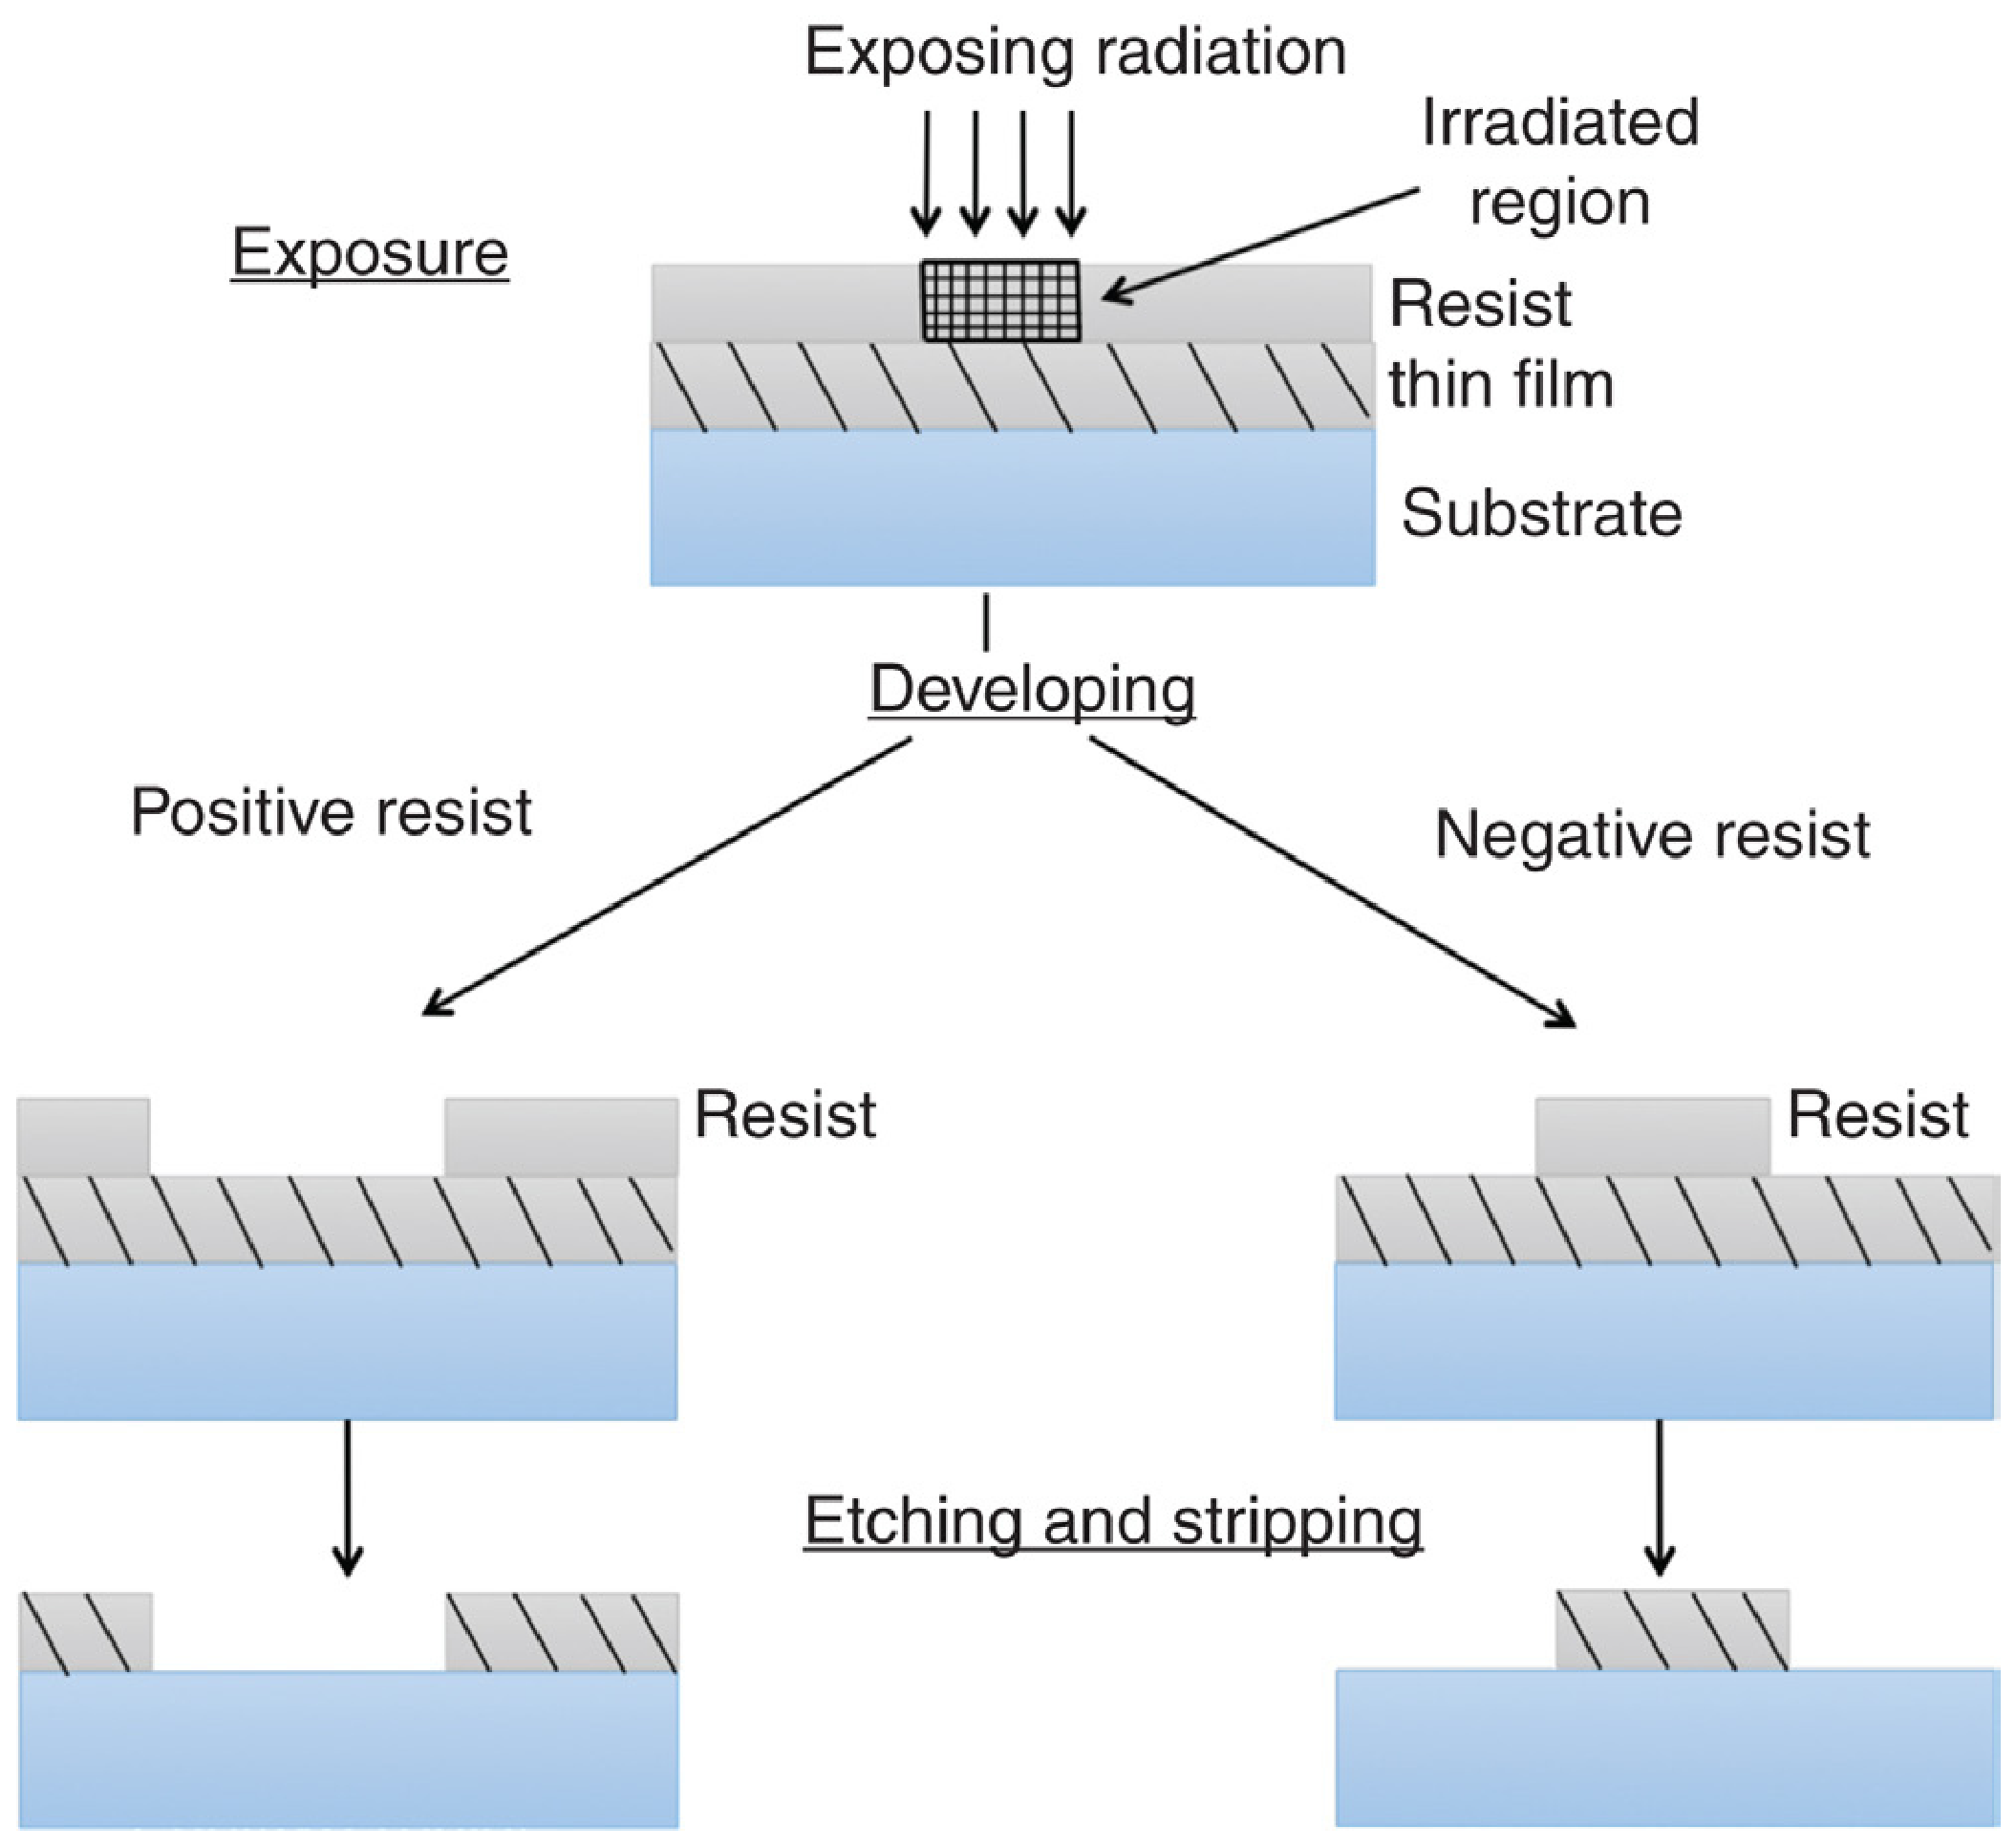
\includegraphics[width=0.6\textwidth]{photoprocess}
\caption[The schematic diagram showing the process of photolithography]{The schematic diagram showing the process of photolithography \cite{ram2018advanced}}
\label{fig:photolithography}
\end{figure}


In this research, the SUSS MA6 mask aligner designed for high-resolution photolithography at the micrometer scale has been applied to transfer patterns from mask to wafer, including mesa patterns, electrode \index{Electrode} patterns, cantilever \index{Cantilever} patterns, etc.

\subsection{Thin film deposition}

Thin Film deposition is the technology of applying a very thin film of material - between a few nanometers to about 100 micrometers, or the thickness of a few atoms – onto a "substrate" surface \index{Substrate} to be coated, or onto a previously deposited coating to form layers. Thin Film deposition is usually divided into two broad categories - chemical deposition and physical vapor deposition coating systems. Chemical deposition is that a volatile fluid precursor produces a chemical change on a surface leaving a chemically deposited coating, such as chemical vapor \index{Deposition!chemical vapor deposition (CVD)} deposition (CVD). Physical vapor deposition (PVD) \index{Deposition!physical vapor deposition (PVD)} refers to a wide range of technologies where a material is released from a source and deposited on a substrate \index{Substrate} using mechanical, electromechanical or thermodynamic processes. The two most common techniques of physical vapor deposition are thermal evaporation and sputtering.

\begin{figure}[H] 
\centering    
\includegraphics[width=0.9\textwidth]{magsup}
\caption[Denton Discovery 635 magnetron sputtering system]{Denton Discovery 635 magnetron sputtering system}
\label{fig:magsup}
\end{figure}

\begin{description}
	\item[Magnetron sputtering]
	
Sputter deposition \index{Deposition!magnetron sputtering} is a physical vapor deposition (PVD) method of thin film deposited by sputtering. The general sputtering method can be used to prepare a variety of materials such as metals, semiconductors, insulators, etc., and has the advantages of simple equipment, easy control, large coating area, and strong adhesion. Sputtering sources often employ magnetrons that utilize strong electric and magnetic fields to confine charged plasma particles close to the surface of the sputter target. In a magnetic field, electrons follow helical paths around magnetic field lines, undergoing more ionizing collisions with gaseous neutrals near the target surface than would otherwise occur. The sputter gas is typically an inert gas such as argon. The plasma can also be sustained at a lower pressure this way.  The certain target atoms near the surface gain sufficient momentum for outward motion and are sputtered out of the target and the sputtered atoms are neutrally charged and so are unaffected by the magnetic trap. These sputtered atoms deposit onto the surface \index{Surface} of the sample to form thin films.

Magnetron sputtering \index{Deposition!magnetron sputtering} includes direct current (DC) magnetron sputtering and radio frequency (RF) magnetron sputtering, each has a different working principle and application objects. The main advantage of RF magnetron sputtering over DC magnetron sputtering is that it does not require the target as an electrode be electrically conductive. Therefore, any material can be sputter-deposited theoretically using RF magnetron sputtering. Magnetron sputtering is advantageous as it doesn’t require evaporation or melting of source materials, allowing for exotic material experimentation and novel coating film applications. Sputter deposition is excellent for materials with high melting points that cannot be evaporated. It can achieve denser coatings than evaporation and is perfect for metallic or insulating coatings with specific optical or electrical properties.

\end{description}

\begin{figure}[H] 
\centering    
\includegraphics[width=0.9\textwidth]{ebeam}
\caption[Denton Vacuum Explore 14 electron beam evaporation system]{Denton Vacuum Explore 14 electron beam evaporation system}
\label{fig:ebeam}
\end{figure}

\begin{description}

	\item[Electron beam evaporation] 
		
E-beam (electron beam) evaporation \index{Deposition!electron beam evaporation} is a thermal evaporation process. E-beam evaporation provides for the direct transfer of a larger amount of energy into the source material, enabling the evaporation of metal and dielectric materials with very high melting temperatures, such as gold and silicon dioxide, respectively.  In e-beam evaporation, the evaporation material can be placed directly in a water-cooled copper hearth or into a crucible and heated by a focused electron beam. Electron beams can be generated by thermionic emission, field electron emission or the anodic arc method. The generated electron beam is accelerated to a high kinetic energy and directed towards the evaporation material. The thermal energy that is produced heats up the evaporation material causing it to melt or sublimate. Once temperature and vacuum level are sufficiently high, vapor will result from the melt or solid. The resulting vapor can then deposits on the substrate to form the required thin film

The deposition rate in this process can be as low as 1 nm per minute to as high as few micrometers per minute. The material utilization efficiency is high relative to other methods, and the process offers structural and morphological control of films, as well as the very high deposition rate. E-Beam evaporations are also advantageous for polymeric coating due to its simplicity and flexibility. E-Beam coatings also process in a more rapid fashion in a batch scenario as compared to Magnetron Sputtered coatings which make them ideal for high-volume commercial applications. E-Beam evaporations work for a wide variety of materials, including those with higher melting points that cannot undergo thermal evaporation, deliver better step coverage than sputtering or chemical vapor deposition (CVD), and offers a higher material utilization efficiency and higher deposition rates than sputtering.
	
\end{description}

In this research, the Denton Discovery 635 magnetron sputtering system has been applied to deposit the magnetic thin film \ce{(Fe90Co10)78Si12B10} in MPD, and the Denton Vacuum Explore 14 electron beam evaporation system has been used to deposit the ohmic and Schottky contact metals \index{Contact!Ohmic contact} in \index{Contact!Schottky contact} both SPD and MPD, including Ti, Al, Au and Ni.

\subsection{Dry etching}

\begin{figure}[H] 
\centering    
\includegraphics[width=0.9\textwidth]{icp}
\caption[SENTECH SI 500 inductively coupled plasma reactive ion etching]{SENTECH SI 500 inductively coupled plasma reactive ion etching}
\label{fig:icp}
\end{figure}


ICP RIE etching \index{Inductively coupled plasma (ICP)} is an advanced technique designed to deliver high etching rates, high selectivity and low damage processing. The gases are introduced above an inductive coil, placed around a ceramic tube. RF is applied to both the coil and chuck to create a plasma. The substrate is placed on the RF-powered chuck, and the wafer takes on potential which accelerates etching species extracted from plasma toward the etched surface. The introduction of different gases can produce different chemical reactions, thereby achieving the purpose of effectively etching different materials. Usually, \ce{SF6}/\ce{Ar}/\ce{O2} gas is used to etch Si and its compound materials, while \ce{BCl3}/\ce{Cl2}/\ce{Ar} gas is widely used to etch GaN and its compound materials. The etching rate can be effectively adjusted by the etching power. This technology combines chemical reaction and ion-induced etching to achieve a high degree of process flexibility. 

In this research, SENTECH SI 500 ICP-RIE plays an important role in the mesa isolation and cantilever \index{Cantilever} structure fabrication process. Especially in the preparation of the cantilever structure, by combining the process design of anisotropic etching \index{Etching!anisotropic etching} of GaN and isotropic etching \index{Etching!isotropic etching} of Si, the cantilevered \index{Cantilever} power MEMS devices with good uniformity and excellent performance has been successfully prepared. It can be determined that ICP-RIE process is the core process technology in the research of GaN power MEMS devices.

\subsection{Rapid thermal processing}

\begin{figure}[H] 
\centering    
\includegraphics[width=0.5\textwidth]{RTP}
\caption[LABSYS RTP-1200 rapid thermal processing system]{LABSYS RTP-1200 rapid thermal processing system}
\label{fig:RTP}
\end{figure}

Rapid thermal processing (RTP) \index{Rapid thermal!processing (RTP)} is a semiconductor manufacturing process which heats silicon wafers to temperatures exceeding 1,000°C for not more than a few seconds. During cooling wafer temperatures must be brought down slowly to prevent dislocations and wafer breakage due to thermal shock. Such rapid heating rates are often attained by high-intensity lamps or lasers. These processes are used for a wide variety of applications in semiconductor manufacturing including dopant activation, thermal oxidation, metal reflow, silicide and barrier metal formation, chemical vapor deposition, and other steps in semiconductor manufacturing.

In this research, LABSYS RTP-1200 RTP is mainly used for ohmic contact formation in AlGaN/GaN HEMTs, and the most commonly used ohmic contact metal composition is Ti/Al/Ni/Au (from surface to bottom).


\section{Characterization techniques}

\subsection{Semiconductor parameter analyzer}

\begin{figure}[H] 
\centering    
\includegraphics[width=0.9\textwidth]{keysight}
\caption[Keysight B1500A semiconductor device parameter analyzer and I-V characteristics of MPD under external magnetic field modulation]{Keysight B1500A semiconductor device parameter analyzer and I-V characteristics of MPD under external magnetic field modulation}
\label{fig:keysight}
\end{figure}

A semiconductor parameter analyzer \index{Semiconductor parameter analyzer} is an all-in-one unit designed to discover the characteristics of semiconductor devices such as diodes, transistors, and thyristors. Based on an oscilloscope, the device also contains voltage and current sources that can be used to stimulate the device under test. The function is to apply a swept (automatically continuously varying with time) voltage to the terminals of the device under test and measure the amount of current that the device permits to flow at each voltage. This V-I (voltage versus current) graph is displayed on an oscilloscope screen. Configuration includes the maximum voltage applied, the polarity of the voltage applied (including the automatic application of both positive and negative polarities), and the resistance inserted in series with the device. The main terminal voltage can often be swept up to several thousand volts, with load currents of tens of amps available at lower voltages.

For two terminal devices such as diodes, the parameter analyzer can display all of the interesting parameters such as the diode's forward voltage, reverse leakage current, reverse breakdown voltage, and so on. For three-terminal devices such as transistors and FETs also use a connection to the control terminal of the device being tested, and the control terminal current or voltage is stepped. By sweeping the voltage through the configured range of main terminal voltages, for each voltage step of the control signal, a group of I-V curves is generated automatically. The parameter analyzers can characterize the electrical characterization of the transistors, diodes, resistors and capacitors that make up semiconductors. 

In this research, the Keysight B1500A semiconductor device parameter analyzer has been widely used to test the electrical properties of AlGaN/GaN HEMTs and power MEMS devices, especially the I-V characteristics under external stimulus.
 

\subsection{Scanning electron microscopy (SEM)}

\begin{figure}[H] 
\centering    
\includegraphics[width=0.45\textwidth]{sem}
\caption[FEI Nova Nano SEM 450 field-emission scanning electron microscopy]{FEI Nova Nano SEM 450 field-emission scanning electron microscopy}
\label{fig:sem}
\end{figure}

A scanning electron microscopy (SEM) \index{Scanning electron microscopy (SEM)} is a type of electron microscope that produces images of a sample by scanning the surface with a focused beam of electrons. The electrons interact with atoms in the sample, producing various signals that contain information about the surface topography and composition of the sample. The signals used by a SEM to produce an image result from interactions of the electron beam with atoms at various depths within the sample. Various types of signals are produced including secondary \index{Secondary electrons (SE)} electrons (SE), reflected or back-scattered electrons \index{Back-scattered electrons (BSE)} (BSE), and transmitted \index{Transmitted electrons} electrons. The electron beam is scanned in a raster scan pattern, and the position of the beam is combined with the intensity of the detected signal to produce an image. Due to the very narrow electron beam, SEM micrographs have a large depth of field yielding a characteristic three-dimensional appearance useful for understanding the surface structure of a sample. There is a wide range of magnifications, from about 10 times to more than 500,000 times, about 250 times the magnification limit of the best light microscopes. Some SEMs can achieve resolutions better than 1 nanometer \cite{reimer2000scanning}.

\begin{figure}[H] 
\centering    
\includegraphics[width=0.6\textwidth]{semgan}
\caption[SEM image of fabricated GaN power MEMS devices]{SEM image of fabricated GaN power MEMS devices}
\label{fig:semgan}
\end{figure}

In this research, FEI Nova Nano SEM 450 field-emission SEM can effectively obtain the topographic features of MEMS devices during fabrication, especially when dry-etching cantilever \index{Cantilever} structures. The accurate grasp of the topographic features greatly improves the efficiency of process development.

\subsection{Transmission electron microscopy (TEM)}

\begin{figure}[ht] 
\centering    
\includegraphics[width=0.5\textwidth]{TEM}
\caption[FEI Tecnai F20 cryo-transmision electron microscope]{FEI Tecnai F20 cryo-transmision electron microscope}
\label{fig:tem}
\end{figure}

Transmission electron microscopy (TEM) \index{Transmission electron microscopy (TEM)} is a microscopy technique in which a beam of electrons is transmitted through a specimen to form an image.  An image is formed from the interaction of the electrons with the sample as the beam is transmitted through the specimen. The image is then magnified and focused onto an imaging device. Transmission electron microscopes are capable of imaging at a significantly higher resolution than light microscopes, owing to the smaller de Broglie wavelength of electrons. This enables the instrument to capture fine detail—even as small as a single column of atoms, which is thousands of times smaller than a resolvable object seen in a light microscope.  What this means is that a TEM is capable of returning an extraordinary variety of nanometer- and atomic-resolution information, in ideal cases revealing not only where all the atoms are but what kinds of atoms they are and how they are bonded to each other. Transmission electron microscopy is a major analytical method in the physical, chemical and biological sciences and is widely used in materials science, nanotechnology and semiconductor research. 

The main difference between SEM and TEM is that SEM creates an image by detecting reflected or knocked-off electrons, while TEM uses transmitted electrons (electrons that are passing through the sample) to create an image. The magnifications that TEMs offer are much higher compared to SEMs. TEM can magnify the samples by more than 50 million times, while for the SEM, this is limited to 1-2 million times. As a result, TEM offers valuable information on the inner structure of the sample, such as crystal structure, morphology and stress state information, while SEM provides information on the sample’s surface and its composition.

\begin{figure}[ht] 
\centering    
\includegraphics[width=0.9\textwidth]{TEMGaN}
\caption[High-resolution TEM image acquired from the AlGaN/AlN/GaN hetero-stacks]{High-resolution TEM image acquired from the AlGaN/AlN/GaN hetero-stacks}
\label{fig:temGaN}
\end{figure}

In this research, FEI Tecnai F20 TEM has been used to characterize the lattice orientation, lattice constants \index{Lattice!constant} and the dislocation defects of GaN, AlN, AlGaN layer.

\subsection{Energy dispersive X-ray spectroscopy (EDX)}

\begin{figure}[H] 
\centering    
\includegraphics[width=0.9\textwidth]{edx}
\caption[Principle of EDX and elemental composition of AlGaN/GaN HEMT characterized by EDX]{Principle of EDX and elemental composition of AlGaN/GaN HEMT characterized by EDX}
\label{fig:edx}
\end{figure}

Energy-dispersive X-ray spectroscopy (EDS, EDX, EDXS or XEDS), \index{Energy-dispersive X-ray spectroscopy (EDX)} is an analytical technique used for the elemental analysis or chemical characterization of a sample. It relies on the interaction of some source of X-ray excitation and a sample. Its characterization capabilities are due in large part to the fundamental principle that each element has a unique atomic structure allowing a unique set of peaks on its electromagnetic emission spectrum. A beam of electrons is focused into the sample to stimulate the emission of characteristic X-rays from a specimen. At rest, an atom within the sample contains ground state (or unexcited) electrons in discrete energy levels or electron shells bound to the nucleus. The incident beam may excite an electron in an inner shell, ejecting it from the shell while creating an electron-hole where the electron was. An electron from an outer, higher-energy shell then fills the hole, and the difference in energy between the higher-energy shell and the lower-energy shell may be released in the form of an X-ray. The number and energy of the X-rays emitted from a specimen can be measured by an energy-dispersive spectrometer. As the energies of the X-rays are characteristic of the difference in energy between the two shells and of the atomic structure of the emitting element, EDS allows the elemental composition of the specimen to be measured \cite{goldstein2017scanning}.

In this research, the EDX equipment is integrated into the transmission electron microscopy equipment to characterize the elemental composition and distribution of AlGaN/GaN HEMTs.

\subsection{High-resolution X-ray diffraction (HRXRD)}

\begin{figure}[ht] 
\centering    
\includegraphics[width=0.6\textwidth]{xrd}
\caption[Bruker D8 DISCOVER high-resolution X-ray diffraction]{Bruker D8 DISCOVER high-resolution X-ray diffraction}
\label{fig:xrd}
\end{figure}

Most of today’s modern semiconductor device structures are epitaxially grown from the gas phase onto a substrate made from silicon, silicon-germanium, III-V and II-VI compounds. These films are nearly-perfect crystalline films containing a relatively low dislocation density. Film properties are largely determined by their compositional and structural parameters. Information such as layer thickness, composition, strain, relaxation and structural quality is obtained by measuring rocking curves and reciprocal space maps using high-resolution X-ray \index{High-resolution X-ray diffraction (HRXRD)} diffraction (HR-XRD). The spatial distribution of defects can also be visualized by X-ray diffraction imaging methods.

The working principle behind HRXRD is \index{Bragg’s law} Bragg’s law, which states that when the x-ray incident onto a crystal surface with an angle of incidence it will reflect back with a same angle of scattering When the path difference is equal to a whole number of wavelength, a constructive interference will occur. The path difference is the separation between the crystal \index{Crystal} planes that caused the reflection. The crystalline structure causes a beam of incident X-rays to diffract into many specific directions. By measuring the angles and intensities of these diffracted beams, HRXRD can be used to analyze the thickness, composition, and strain state of epitaxial single-crystal thin films, and can also measure the density of defects in epitaxial layers by FWHM of Bragg reflections obtained in the direction perpendicular to the diffraction vector.

\begin{figure}[ht] 
\centering    
\includegraphics[width=0.9\textwidth]{xrdhemt}
\caption[The X-ray diffraction spectra of GaN HEMT]{The X-ray diffraction spectra of GaN HEMT}
\label{fig:xrdhemt}
\end{figure}

In this research, Bruker D8 DISCOVER HR-XRD has been used to measure the composition, defects and thickness of GaN Wafer.

\subsection{Raman spectroscopy}

\begin{figure}[H] 
\centering    
\includegraphics[width=0.9\textwidth]{raman}
\caption[HORIBA LabRAM HR Evolution Raman spectroscopy]{HORIBA LabRAM HR Evolution Raman spectroscopy}
\label{fig:raman}
\end{figure}

Raman scattering \index{Raman!scattering} is an extremely powerful contactless tool which allows non-destructive and quantitative microanalysis of structural and electrical properties of semiconductor materials. This technique is very useful since the Raman signal is very sensitive to the microstructural state of the sample and other local environments, therefore giving information on the structure of the material on the scale of a few lattice \index{Lattice!constant} constants. 

 Raman is a light scattering technique, whereby a molecule scatters incident light from a high-intensity laser light source. Most of the scattered light is at the same wavelength as the laser source and does \index{Rayleigh scattering} not provide useful information – this is called Rayleigh Scattering. However, a small amount of light (typically 0.0000001$\%$) is scattered at different wavelengths, which depend on the chemical structure of the analyte – this is called Raman \index{Raman!scattering} Scattering. Raman signal is a function of the electron-phonon interaction, i.e. lattice vibration. A Raman spectrum features a number of peaks, showing the intensity and wavelength position of the Raman scattered light. Each peak corresponds to a specific lattice vibration. Raman spectroscopy \index{Raman!spectroscopy} probes the chemical structure of a material and provides information about chemical structure and identity, phase and polymorphism, intrinsic stress/strain and contamination and impurity \cite{smith2019modern}.
 
\begin{figure}[H] 
\centering    
\includegraphics[width=1\textwidth]{ramanGaN}
\caption[Principle of Raman spectroscopy and Raman spectroscopy of GaN-on-Si wafers]{Principle of Raman spectroscopy and Raman spectroscopy of GaN-on-Si wafers}
\label{fig:ramangan}
\end{figure}

In this research, changes in the intrinsic lattice strain between AlGaN, AlN, and GaN layers during the fabrication of MEMS devices can be detected by HORIBA LabRAM HR Evolution Raman spectroscopy, which would greatly affects the material properties and electrical properties of MEMS devices.


\section{Summary}

In this chapter, a brief overview of the semiconductor fabrication and characterization equipment used in the manufacturing of GaN power MEMS is given. The equipment is briefly classified according to different functions such as deposition, etching, lithography, etc., and the specific models of the equipment, the basic working principle and the main use in this research are described. The independent processes of these devices with different functions are integrated to complete the preparation of GaN power MEMS, which becomes the basis of process integration in \autoref{ch:Process Development and Integration of Power MEMS Devices}.


\nomenclature[z-TEM]{TEM}{Transmission electron microscopy}
\nomenclature[z-SEM]{SEM}{Scanning electron microscopy}
\nomenclature[z-HAADF-STEM]{HAADF-STEM}{High-angle annular dark-field scanning transmission electron microscopy}
\nomenclature[z-EDX]{EDX}{Energy dispersive X-ray spectroscopy}
\nomenclature[z-MOCVD]{MOCVD}{Metal organic compound chemical vapor deposition}
\nomenclature[z-MOVPE]{MOVPE}{Metal organic vapor phase expitaxy}
\nomenclature[z-ICP-RIE]{ICP-RIE}{Inductively coupled plasma reactive ion etching}
\nomenclature[z-CVD]{CVD}{chemical vapor deposition}
\nomenclature[z-PVD]{PVD}{Physical vapor deposition}
\nomenclature[z-XRD]{XRD}{X-ray diffraction}
\nomenclature[z-RTP]{RTP}{Rapid thermal processing}
\nomenclature[z-UV]{UV}{Ultraviolet}
\nomenclature[z-EUV]{EUV}{Extreme ultraviolet}
\nomenclature[z-E-Beam]{E-Beam}{Electron beam}
\nomenclature[z-DC]{DC}{Direct current}
\nomenclature[z-RF]{RF}{Radio frequency}
\nomenclature[z-UID]{UID}{Unintentionally doped}



\chapter{Process Development and Integration of Power MEMS Devices}
\label{ch:Process Development and Integration of Power MEMS Devices}

% **************************** Define Graphics Path **************************
\ifpdf
    \graphicspath{{Chapter7/Figs/Raster/}{Chapter7/Figs/PDF/}{Chapter6/Figs/}}
\else
    \graphicspath{{Chapter7/Figs/Vector/}{Chapter7/Figs/}}
\fi


In this chapter, I would develop the corresponding fabrication process parameters and their process integration based on the manufacturing technology and equipment in Chapter Three, thus realizing the whole process \index{Fabrication process} from GaN wafer to device. In order to simplify the expression of the process and clarify the steps of the process, this chapter uses different codes to represent the different steps and their meanings. For example MESA.3) indicates that this process is the third step in the mesa preparation process, and [AE-N] indicates the alignment and exposure of negative photoresist. The process that first appears in this chapter would be described in detail about the main purpose of the process, the equipment used, and the detailed recipe parameters and shorthand code, while the same process in the following steps is only represented by the shorthand code. I've listed every step without omission based on shorthand code. Moreover, in order to visualize the fabrication process flow, a corresponding flow chart has been drawn to illustrate the main process steps.

\section{Process flow and recipe}

\begin{figure}[H] 
\centering    
\includegraphics[width=0.8\textwidth]{processflow}
\caption[The schematic diagram of process flow]{The schematic diagram of process flow}
\label{fig:processflow}
\end{figure}

The fabrication process flow chart of GaN power MEMS is shown in the \autoref{fig:processflow}, which can be roughly divided into four main steps. The first step is mesa isolation, and the device is isolated by ICP etching. The second step is to deposit the source, drain and gate metal electrodes to realize the HEMT device. The third step is the deposition of the magnetic thin film at the front end of the cantilever (there is no such step for the SPD device). The fourth step is to etch the cantilever structure. The realization of each step is inseparable from the pattern transfer of photomask, so \autoref{fig:layout} shows the layout (drawn with AutoCAD) during the fabrication. The specific steps will be described in detail in the subsections.

\begin{figure}[H] 
\centering    
\includegraphics[width=0.9\textwidth]{mask}
\caption[Layout of GaN power MEMS devices]{Layout \index{Photomask} of GaN power MEMS devices}
\label{fig:layout}
\end{figure}


\subsection{Wafer growth}

\begin{figure}[H] 
\centering    
\includegraphics[width=0.7\textwidth]{structure}
\caption[GaN-on-SiC wafer hetero-epitaxial structure]{GaN-on-SiC wafer hetero-epitaxial structure}
\label{fig:structure}
\end{figure}


The \index{Fabrication process} epitaxial growth \index{Epitaxial!growth} of GaN wafer \index{Wafer} is a fundamental step in the research of group III nitride semiconductors. Due to the difficulty in obtaining large-scale and high-quality GaN bulk substrates, GaN epitaxial layers are still mainly grown on foreign substrates. The most widely used are sapphire, SiC, and Si. which have a large lattice mismatch \index{Lattice!mismatch} with GaN. To address this problem, Amano et al. developed a two-step growth method in 1986. The AlN nucleation layer is first grown at low temperature, and then raised to high temperature to grow GaN layer, which greatly improves the quality of the GaN epitaxial layer \cite{amano1986metalorganic}. In 1989, Akasaki et al. systematically studied and improved the two-step method, first using low temperature to deposit AlN or GaN as a buffer layer, and then desired GaN material is grown on the buffer layer in a high temperature environment \cite{akasaki1989effects}.

The \index{Fabrication process} hetero-expitaxial structure of 3-inch GaN-on-Si wafer is shown in \autoref{fig:structure}. From bottom to top are 1 \unit{mm} Si(111) substrate, 3.5 $\sim$ 4 \unit{\um} AlN/AlGaN multi-layer buffer layer, 400 $\sim$ 600 \unit{\nm} unintentionally doped (UID) GaN buffer layer, 300 \unit{\nm} intrinsic GaN 2DEG channel layer, 1 \unit{\nm} AlN barrier layer, 20 \unit{\nm} AlGaN barrier layer and 2 \unit{\nm} GaN cap layer. The lattice mismatch between the Si substrate and the GaN 2DEG channel layer is alleviated by different Al composition of the AlN/AlGaN buffer layer, and the lattice mismatch between the AlN/AlGaN layer and the GaN 2DEG \index{Two-dimensional electron gas (2DEG)} channel \index{Channel} layer is further adjusted by the UID GaN buffer layer. The grown wafer exhibits good electrical performance with 300 \unit{\ohm}/square  sheet resistance, \num{1.00e13} \unit{\per\square\cm} carrier \index{Carrier!concentration} density, 2000 \unit{cm^2/(Vs)} mobility \index{Electron mobility} and \SI{600}{\volt} breakdown \index{Voltage!breakdown voltage} voltage.

\subsection{Pre-processing}
During \index{Fabrication process} pre-processing, the dice \index{Dice} of size \numproduct{2 x 2} \unit{mm} and \numproduct{3 x 3} \unit{mm} firstly have been cut from the grown 3-inch wafers with the DISCO DAD3350 automatic dicing saw. Because there are a lot of particles and organic contaminants on the surface \index{Surface} of the cut dice, the dice would be then strictly cleaned by cleaning technologies. The recipe is listed here:

\begin{description}
	\item[PRE.1)] Wafer \index{Dice} dicing [WD].
	\item[PRE.2)] A complete RCA cleaning \index{Cleaning!RCA cleaning} process ($\times$ 1 time) [WET-RCA].
	\item[PRE.3)] Piranha solution \index{Piranha solution} with the \ce{H2SO4} (98$\%$) and \ce{H2O2} (30$\%$) in 7:3 ratios, sonicated for 10 minutes ($\times$ 1 time) [WET-PA].
	\item[PRE.4)] Sonicate in acetone solution for 5 minutes ($\times$ 3 times) [WET-ACE].
	\item[PRE.5)] Sonicate in \index{Cleaning!wet cleaning} ethanol solution for 5 minutes ($\times$ 3 times) [WET-ETH].
	\item[PRE.6)] Sonicate in deionized water \index{Deionized water} for 5 minutes ($\times$ 3 times) [WET-DIW].
	\item[PRE.7)] Sonicate in hydrochloric acid \index{Hydrochloric acid} for 5 minutes ($\times$ 3 times) [WET-HC].
	\item[PRE.8)] [WET-DIW]
	\item[PRE.9)] Nitrogen gas drying [GD-N].
	\item[PRE.10)] Dry cleaning \index{Cleaning!dry cleaning} in PVA TePla IoN 40 plasma cleaner with 80 sccm Oxygen gas and \SI{100}{\watt} power for 1 min ($\times$ 1 time) [DC-OX].
\end{description}


\subsection{Mesa preparation}

In \index{Fabrication process} order \index{Photoresist} to isolate different devices on a single die, mesa \index{Mesa isolation} isolation, often referred to as active area \index{Active region} isolation, is required. We first transfer the active area pattern from photomask \index{Photomask} to \index{Dice} dice by \index{Photolithography} photolithography, and then etch the mesa by ICP-RIE. The size of the active area \index{Active region} is \numproduct{34 x 34} \unit{um^2}, and the photomask is prepared as shown in the \autoref{fig:active area}, where the cross pattern marks are mainly used for subsequent overlay alignment. The main steps are as follows:

\begin{description}

	\item[MESA.1)] Photoresist coating
	
	Spin coating SUN-9i \index{Photoresist} negative photoresist produced by Suntific Material (Weifang), Ltd. The rotation speed is 500 rpm/min for the first 8 seconds and 5000 rpm/min for the last 40 seconds [PC-N].
	
	\item[MESA.2)] Post-apply bake
	
	After \index{Fabrication process} coating, the resulting resist film will contain between 20$\%$ $\sim$ 40$\%$ by weight solvent. The post-apply bake \index{Post-apply bake} process, also called a soft-bake or a pre-bake, involves drying the photoresist after spin coating by removing this excess solvent. The main reason for reducing the solvent content is to stabilize the photoresist film \cite{mack2008fundamental}. In this process, the post-apply baking recipe is \SI{110}{\degreeCelsius} for 60 seconds [PAB-N].
	
	\item[MESA.3)] Alignment and exposure
	
\begin{figure}[H] 
\centering    
\includegraphics[width=0.9\textwidth]{active area}
\caption[Photomask of active area]{Photomask \index{Photomask} of active area}
\label{fig:active area}
\end{figure}
	
	Align and exposure with SUSS MA6 mask aligner, and exposure parameters are as follows: Process: Lithography, Exposure time: 30 seconds, Alignment gap: 50 \unit{um}, Contact type: Soft, WEC type: Cont, WEC-offset: OFF [AE-N].
	
	\item[MESA.4)] Post-exposure bake
	
	Post-exposure bake \index{Post-exposure bake} is one method of reducing the standing wave effect \cite{mack2008fundamental}. The recipe is \SI{140}{\degreeCelsius} for 60 seconds [PEB-N].
	
	\item[MESA.5)] Development
	
	Once \index{Photoresist} exposed, the photoresist \index{Photoresist} must be developed. The aqueous and tetramethyl ammonium hydroxide (TMAH) are commonly used as developers. Development is undoubtedly one of the most critical steps in the photoresist process. The characteristics of the resist-developer interactions determine to a large extent the shape of the photoresist profile and, more importantly, the linewidth control \cite{mack2008fundamental}. The development recipe is to first stir and soak in developer solution \index{Developer solution} SUN-238D produced by Suntific Material (Weifang), Ltd for 40 seconds, and then stir and soak in \index{Deionized water} deionized water for 20 seconds [DEV-N].	
	
	\item[MESA.6)] [GD-N]
	
	\item[MESA.7)] [DC-OX]
	
	\item[MESA.8)] ICP-RIE etching
	 
	 In \index{Fabrication process} order \index{Photoresist} to isolate the \index{Mesa isolation} mesa, all epitaxial layers above the AlN/AlGaN multi-layer buffer layer except the active area \index{Active region} must be removed, including UID GaN buffer layer, intrinsic GaN 2DEG \index{Two-dimensional electron gas (2DEG)} channel \index{Channel} layer, AlN barrier layer, AlGaN barrier layer and GaN cap layer. The total etching thickness is about 1000 \unit{\nm}. The etching process has been performed with SENTECH SI 500 ICP-RIE \index{Inductively coupled plasma (ICP)} and the etching recipe is as follows: Etching gas: \ce{BCl3}/\ce{Cl2}/\ce{O2} (10/32/5 sccm), Etching power: \SI{550}{\watt}, RF power: \SI{100}{\watt}. The etching rate is 200 \unit{nm/min}, and the total etching time is 10 minutes [DE-MESA].
	 
	\item[MESA.9)] [WET-ACE]
	
	\item[MESA.10)] [WET-ETH]
	
	\item[MESA.11)] [WET-DIW]
	
	\item[MESA.12)] [GD-N]
	
	\item[MESA.12)] [DC-OX]
		
\end{description}


\subsection{Metal-semiconductors contact formation}

After \index{Fabrication process} the isolation \index{Mesa isolation} of the \index{Active region} active region, the next step begins to prepare the gate Schottky contact \index{Contact!Schottky contact} and the source-drain \index{Contact!Ohmic contact} ohmic contact. The source-drain ohmic contact would been prepared first, with an area of \numproduct{6 x 34} \unit{um^2}. By depositing Ti, Al, Ni, Au metals in sequence and undergoing rapid thermal \index{Rapid thermal!annealing (RTA)} annealing, a good ohmic contact has been formed on the GaN \index{Surface} surface. The Schottky contacts are then further formed by depositing Ni and Au, with an area of \numproduct{5 x 34} \unit{um^2}. The prepared gate contact has good control performance on electrons in the channel. For the convenience of subsequent electrical tests, the photomask \index{Photomask} of the contact also includes a pad with a much larger area (about \numproduct{1000 x 1000} \unit{um^2}).

\begin{description}

	\item[CTC.1)] [PC-N]
	\item[CTC.2)] [PAB-N]
	\item[CTC.3)] [AE-N]
	
\begin{figure}[H] 
\centering    
\includegraphics[width=0.9\textwidth]{source}
\caption[Photomask of source and drain contact]{Photomask \index{Photomask} of source and drain contact}
\label{fig:source}
\end{figure}

	\item[CTC.4)] [PEB-N]
	
	\item[CTC.5)] [DEV-N]
	
	\item[CTC.6)] [GD-N]
	
	\item[CTC.7)] [DC-OX]
	
	\item[CTC.8)] Source-drain metal deposition
	
	The \index{Fabrication process} source-drain \index{Photoresist} contact metal is Ti, Al, Ni, Au. Ti is a barrier metal and must have a work function (3.95 \unit{\eV}) that approximates the affinity potential of GaN (4.11 \unit{\eV}), and therefore is the most widely used barrier metal. Al is a commonly used capping layer, its work function is 4.25 \unit{\eV}, and it can also promote the solid-phase chemical reaction between N atoms and the barrier metal Ti. Ni acts as a diffusion barrier metal, preventing the interdiffusion of the cap layer metal Au and the barrier layer metal Al to the surface \index{Surface} of the GaN material. Au is a stable, low-resistance noble metal ideal for use as a cap layer metal.
	
	In this research, from the bottom (GaN surface) to the top, Ti with a thickness of 20 \unit{\nm}, Al with a thickness of 120 \unit{\nm}, Ni with a thickness of 45 \unit{\nm}, and Au with a thickness of 55 \unit{\nm} have been deposited using Denton Vacuum Explore 14 E-beam evaporation system at deposition rates of \SI{0.5}{\angstrom}/s, \SI{1}{\angstrom}/s, \SI{0.5}{\angstrom}/s and \SI{0.5}{\angstrom}/s, respectively [DEP-SD].
	
	\item[CTC.9)] [WET-ACE]
	
	\item[CTC.10)] [WET-ETH]
	
	\item[CTC.11)] [WET-DIW]
	
	\item[CTC.12)] [GD-N]
	
	\item[CTC.13)] [DC-OX]
	
	\item[CTC.14)] Rapid thermal processing
	
	Rapid \index{Fabrication process} thermal \index{Rapid thermal!processing (RTP)} processing (RTP) \index{Rapid thermal!annealing (RTA)} of the deposited Ti, Al, Ni, Au metal is necessary in order to form an \index{Contact!Ohmic contact} ohmic contact. In this work, rapid thermal annealing at \SI{850}{\degreeCelsius} for 30 seconds has been performed using a LABSYS RTP-1200 rapid thermal processing system [RTP-OHM].
	
	\item[CTC.15)] [WET-ACE]
	
	\item[CTC.16)] [WET-ETH]
	
	\item[CTC.17)] [WET-DIW]
	
	\item[CTC.18)] [GD-N]
	
	\item[CTC.19)] [DC-OX]
	
	\item[CTC.20)] [PC-N]
	\item[CTC.21)] [PAB-N]
	\item[CTC.22)] [AE-N]
	
\begin{figure}[H] 
\centering    
\includegraphics[width=0.9\textwidth]{gate}
\caption[Photomask of gate contact]{Photomask \index{Photomask} of gate contact}
\label{fig:gate}
\end{figure}
	
	\item[CTC.23)] [PEB-N]
	
	\item[CTC.24)] [DEV-N]
	
	\item[CTC.25)] [GD-N]
	
	\item[CTC.26)] [DC-OX]
	
	\item[CTC.27)] Gate metal deposition

	The \index{Photoresist} gate \index{Contact!Schottky contact} contact metal is Ni, Au from the bottom (GaN surface) to the top. Ni with a thickness of 80 \unit{\nm}, and Au with a thickness of 50 \unit{\nm} have been successively deposited using Denton Vacuum Explore 14 E-beam evaporation system at deposition rates of \SI{0.5}{\angstrom}/s and \SI{0.5}{\angstrom}/s, respectively [DEP-G].
		
	\item[CTC.28)] [WET-ACE]
	
	\item[CTC.29)] [WET-ETH]
	
	\item[CTC.30)] [WET-DIW]
	
	\item[CTC.31)] [GD-N]
	
	\item[CTC.32)] [DC-OX]
	
\end{description}

Until \index{Fabrication process} now, I have prepared an AlGaN/AlN/GaN \index{HEMT} HEMT device on \index{Wafer} GaN-on-Si wafer. The active region \index{Active region} is \numproduct{34 x 34} \unit{um^2}, the gate is a Ti/Au Schottky contact with a width of 5 \unit{um}, and the source and drain are Ti/Al/Ni/Au ohmic \index{Contact!Ohmic contact} contact with a width of 6 \unit{um}. The electrical characteristics of HEMT are shown in the \autoref{fig:performancehemt}. It can be seen from the figure that HEMT exhibits good Schottky contacts \index{Contact!Schottky contact} on the gate and ohmic contacts on the source and drain (\autoref{fig:performancehemt}c,d). Based on the good electrical contact performance, the output characteristics ($I_{ds}-V_{ds}$) of HEMT have excellent gate control capabilities, as shown in \autoref{fig:performancehemt}a. Therefore, the output current \index{Output!current} exhibits good linearity at low source-drain bias ($V_{ds}$) voltage, and then as the bias voltage further increases, the output current reaches saturation. HEMT can achieve stable large current output in the saturation region, and can be effectively controlled at various \index{Voltage!gate voltage} gate voltage $V_{gs}$ from \SI{-7}{\volt} to \SI{1}{\volt}. The maximum current density at \SI{1}{\volt} gate voltage reaches 304 \unit{\mA\per\mm}, and the maximum transconductance \index{Transconductance} reaches 42.4 \unit{\milli\siemens\per\mm}, showing excellent electrical performance. Moreover, the gate leakage current \index{Current!leakage current} and source-drain leakage current of HEMT are also within a \index{Fabrication process} reasonable range (\autoref{fig:performancehemt}e,f).

\begin{figure}[H] 
\centering    
\includegraphics[width=0.9\textwidth]{performancehemt}
\caption[Electrical performance of fabricated AlGaN/AlN/GaN HEMTs]{Electrical performance of fabricated AlGaN/AlN/GaN HEMTs}
\label{fig:performancehemt}
\end{figure}



\subsection{Magnetic thin film deposition (For MPD)}

Before \index{Fabrication process} the \index{Photoresist} preparation of cantilever, there is one more process which is unique to \index{Magnetosensory power MEMS devices (MPD)} MPD. This process aims to deposit a magnetic \index{Magnetic!thin film} thin film \index{Thin film} on the top half \index{Cantilever} of the cantilever, which can generate magnetic forces in different directions at the front of the cantilever under the action of external \index{Magnetic!field} magnetic field. The size of the mask is \numproduct{175 x 60} \unit{um^2}, and it is located in the front half of the cantilever, where the size of the cantilever is \numproduct{350 x 60} \unit{um^2}. 

\begin{description}
	\item[MAG.1)] [PC-N]
	\item[MAG.2)] [PAB-N]
	\item[MAG.3)] [AE-N]

\begin{figure}[H] 
\centering    
\includegraphics[width=0.9\textwidth]{magnetic film}
\caption[Photomask of magnetic film]{Photomask \index{Photomask} of magnetic film}
\label{fig:magnetic film}
\end{figure}

	\item[MAG.4)] [PEB-N]
	
	\item[MAG.5)] [DEV-N]
	
	\item[MAG.6)] [GD-N]
	
	\item[MAG.7)] [DC-OX]
	
	\item[MAG.8] Magnetic thin film deposition
	
	The \index{Photoresist} Denton Discovery 635 magnetron sputtering \index{Deposition!magnetron sputtering} system has been applied to deposit 500 \unit{\nm} thick \index{Magnetic!thin film} magnetic thin film \ce{(Fe90Co10)78Si12B10}. The recipe is as follow: DC sputtering, Gas: Ar 135 sccm, Power: \SI{400}{\watt}, Pressure: 7.2 mtorr. The deposition rate is 15 \unit{nm/min}, and the deposition time is 33.3 min [DEP-MAG].
	
	\item[MAG.9)] [WET-ACE]
	
	\item[MAG.10)] [WET-ETH]
	
	\item[MAG.11)] [WET-DIW]
	
	\item[MAG.12)] [GD-N]
	
	\item[MAG.13)] [DC-OX]
	

\end{description}

\subsection{GaN cantilever preparation}

Finally, the \index{Fabrication process} ICP-based \index{Inductively coupled plasma (ICP)} dry \index{Photoresist} etching has been performed by combing the \index{Etching!isotropic etching} anisotropic/isotropic etching \index{Etching!anisotropic etching} to fabricate the \index{Cantilever} cantilever. The main steps of the etching process are as follows: Step 1: anisotropic etching of photoresist patterned GaN (thickness: 5 \unit{\um}). Step 2: isotropic etching of Si to release the cantilever. The manufactured cantilever has dimensions of \numproduct{350 x 60 x 5} \unit{um^3}. For the final fabricated \index{MEMS} MEMS devices, the SPD has only a single cantilever, while the MPD has a cantilever with a magnetic thin film in the front half end.
	
\begin{description}

	\item[CAN.1)] Photoresist coating
	
	Spin coating AZ4620 positive photoresist produced by Suntific Material (Weifang), Ltd. The rotation speed is 500 rpm/min for the first 8 seconds and 3500 rpm/min for the last 60 seconds [PC-P].
	
	\item[CAN.2)] Post-apply bake
	
	The pre-baking \index{Post-apply bake} recipe is \SI{95}{\degreeCelsius} for 3 minutes [PAB-P].
	
	\item[CAN.3)] [PC-P]
	

	\item[CAN.4)] [PAB-P]
	
	
	\item[CAN.5)] Alignment and exposure
	
\begin{figure}[H] 
\centering    
\includegraphics[width=0.9\textwidth]{cantilever}
\caption[Photomask of GaN cantilever]{Photomask of GaN cantilever}
\label{fig:cantilever}
\end{figure}

	Align \index{Cantilever} and exposure \index{Photomask} with SUSS MA6 mask aligner, and exposure parameters are as follows: Process: Lithography, Exposure time: 54 seconds, Alignment gap: 30 \unit{\um}, Contact type: Soft, WEC type: Cont, WEC-offset: OFF [AE-P].

	\item[CAN.6)] Development
	
	The \index{Fabrication process} developing \index{Photoresist} recipe is firstly immersed in a 3:1 solvent of deionized \index{Deionized water} water \index{Developer solution} and developer solution AZ-400K produced by Santaifu Materials (Weifang), Ltd, and then stirred and immersed in deionized water. The time needs to be determined in real time according to the real-time observation of the optical microscope (about 4 $\sim$ 5 \unit{\minute}) [DEV-P].
	
	\item[CAN.7)] [GD-N]
	
	\item[CAN.8)] [DC-OX]
	
	\item[CAN.9)] ICP-RIE etching

	 To \index{Fabrication process} fabricate the \index{Cantilever} cantilever, an anisotropic etching \index{Etching!anisotropic etching} must first be performed to etch the GaN, AlN and AlGaN layers, and then an isotropic \index{Etching!isotropic etching} etching of Si must be performed to release the cantilever. The etching process is performed with SENTECH SI 500 ICP-RIE. Firstly, the GaN etching recipe is as follows: Etching gas: \ce{BCl3}/\ce{Cl2}/\ce{Ar} (10/32/5 sccm), Etching power: \SI{550}{\watt}, RF power: \SI{100}{\watt}. The etching rate is 200 \unit{nm/min}, and the total etching time is 25 min. Secondly, the Si etching recipe is as follows: Etching gas: \ce{SF6}/\ce{O2}/\ce{Ar} (30/5/10 sccm), Etching power: \SI{800}{\watt}, RF power: \SI{50}{\watt}. The lateral etching rate is 2 \unit{um/min}, and the total etching time is 25 min [DE-CAN].
	 
	 \item[CAN.10)] [DC-OX]	

\end{description}

In this section, I have successfully prepared the GaN power \index{MEMS} MEMS devices with cantilever \index{Cantilever} structure. The electrical characteristics of MPD are shown in the \autoref{fig:performancempd}. MPD \index{Magnetosensory power MEMS devices (MPD)} exhibits electrical properties similar to \index{HEMT} HEMT. However, compared with HEMT, the current of MPD under the bias voltage of \SI{10}{\volt} is reduced by 60.5 \unit{\mA\per\mm}. The gate leakage current \index{Current!leakage current} and source-drain leakage current of MPD are also slightly larger than HEMT, as shown in \autoref{fig:performancempd}e,f. Furthermore, the transfer ($I_{ds}-V_{gs}$) characteristics of the MPD at $V_{ds}$ = \SI{10}{\volt} has also been measured. The maximum transconductance \index{Transconductance} ($g_{m, max}$) of MPD is 32.9 \unit{\milli\siemens\per\mm} (\autoref{fig:performancempd}b), while the value for the HEMT can reach 42.4 \unit{\milli\siemens\per\mm} (\autoref{fig:performancehemt}b). Therefore, the transconductance performance of MPD is also slightly lower than HEMT due to the performance degradation \index{Degradation} caused by dry etching process. 

It can be concluded that, compared with the HEMT device before etching, the performance of the MPD device is reduced by about 30$\%$. This is because the long-term ICP \index{Inductively coupled plasma (ICP)} etching weakens the contact performance of the \index{Electrode} electrode, and the removal of the Si \index{Substrate} substrate releases the lattice strain \index{Lattice!strain} of AlGaN/AlN/GaN \index{AlGaN/AlN/GaN heterojunction} heterojunction. This is also because the dry etching \index{Etching!dry etching} process has caused damage to the lattice structure of the material. The performance degradation \index{Degradation} of MEMS devices before and after etching is discussed in detail in the \index{Cantilever} next \index{Fabrication process} subsection.

\begin{figure}[H] 
\centering    
\includegraphics[width=0.9\textwidth]{performancempd}
\caption[Electrical performance of fabricated MPD]{Electrical performance of fabricated \index{Magnetosensory power MEMS devices (MPD)} MPD}
\label{fig:performancempd}
\end{figure}

\section{Mechanisms of process-induced performance degradation}

This \index{Fabrication process} section briefly discusses the physical mechanisms \index{Physical!mechanism} of MEMS device performance degradation \index{Degradation} before and after the ICP-RIE \index{Inductively coupled plasma (ICP)} etching process. By means of Raman spectroscopy \index{Raman!spectroscopy} and literature review, the effects of lattice strain \index{Lattice!strain} release and introduction of lattice defects \index{Lattice!defects} during the cantilever \index{Cantilever} fabrication process on device performance have been revealed respectively.

\subsection{Lattice strain relief and piezoelectric effect}

\begin{figure}[H] 
\centering    
\includegraphics[width=0.7\textwidth]{ramanmpd}
\caption[Raman spectroscopy of fabricated HEMT and MPD]{Raman spectroscopy of fabricated HEMT and MPD}
\label{fig:ramanmpd}
\end{figure}

In order to reveal the physical mechanism \index{Physical!mechanism} of process-induced performance loss, the Raman spectroscopy tests on both HEMT \index{HEMT} and MPD \index{Magnetosensory power MEMS devices (MPD)} at room temperature have been performed to explain the influence of the ICP dry etching \index{Etching!dry etching} process on the electrical performance of MEMS, as shown in \autoref{fig:ramanmpd}. It exhibits that the $E_{2h}$ phonon mode of MPD shows a blue shift from 568.31 \unit{\per\cm} to 569.33 \unit{\per\cm} compared with the HEMT, which reveals that the dry etching process releases the silicon substrate and relaxes the tensile strain of the GaN layer \cite{yang2015influence,wang2016piezotronic}. The relationship between the biaxial stress \index{Biaxial stress model} and the shift of the Raman phonon frequency is shown in \autoref{eq:raman} 
\begin{equation}
\sigma _{a}=\frac{\Delta \omega}{K_{\mathrm{RS}}^{\mathrm{E} 2(h i g h)}}
\label{eq:raman}
\end{equation}
where $\sigma _{a}$ is the \index{In-plane biaxial stress} in-plane biaxial stress, $\Delta \omega$ is the shift of the Raman \index{Raman!phonon frequency} phonon frequency, and $K_{\mathrm{RS}}^{\mathrm{E} 2(h i g h)}$ is the Raman biaxial stress conversion \index{Raman!biaxial stress conversion factor} factor. We can obtain that the tensile strain of the GaN epitaxial layer \index{Epitaxial!layer} is reduced by 352 \unit{\MPa} compared with that on the Si \index{Substrate} substrate \cite{choi2013analysis}. According to the \index{Piezoelectric!effect} piezoelectric effect, the removal of the Si substrate partially releases the lattice \index{Lattice!strain} strain of the GaN layer, thereby changing the piezoelectric polarization charge \index{Piezoelectric!polarization charge} of the GaN layer, adjusting the energy band \index{Energy band} of the heterostructure, and finally reducing the density of 2DEG \index{Two-dimensional electron gas (2DEG)} in the \index{AlGaN/AlN/GaN heterojunction} AlGaN/AlN/GaN heterojunction.

\subsection{Lattice defects and Schottky contact degradation}

In \index{Fabrication process} addition, a large number of lattice defects \index{Lattice!defects} have also been introduced during the \index{Etching!dry etching} dry etching process, which reduces the electrical performance of MPD \index{Magnetosensory power MEMS devices (MPD)} to a certain extent \cite{ladroue2010deep,pearton2000review,huang2004inductively}. Moreover, it has been reported that the \index{Inductively coupled plasma (ICP)} ICP etching could introduce lattice defects and surface state to the AlGaN/AlN/GaN heterojunction \index{AlGaN/AlN/GaN heterojunction} and massive damage to contact \index{Electrode} electrode, which will form electron trap levels. This will result in the increase of ideality factor and the leakage current, thereby significantly reducing the gate control ability \cite{cao2000schottky,choi2003observation,fang2003etching,JieLiu2007Influence}. Last but not least, the etching of the Si substrate under the cantilever will also greatly weaken the heat dissipation in the active area. All these effects enhance the self-heating effect \index{Self-heating effect} of the \index{MEMS} MEMS device, thus impairing the \index{Output!current} output current performance \cite{yang2011high,hajjiah2020effect,greco2017temperature}.

In summary, ICP \index{Inductively coupled plasma (ICP)} dry etching could inevitably degrade \index{Degradation} the performance of \index{MEMS} MEMS during the preparation of the \index{Cantilever} cantilever. Comparing the performance of \index{Magnetosensory power MEMS devices (MPD)} MPD and \index{HEMT} HEMT, it can be concluded that due to the ICP etching process in the cantilever fabrication process, the electrical performance of MPD has been degraded to a certain extent compared to HEMT devices. It has shown that this performance degradation \index{Degradation} is unavoidable in the process of fabricating cantilever \index{Cantilever} structures using the ICP process, but we have improved the performance degradation during cantilever \index{Cantilever} fabrication through process optimization. Compared to the electrical performance of SPD \index{Strain-controlled power MEMS devices (SPD)} in \autoref{ch:Strain-controlled power devices}, the electrical performance of \index{Magnetosensory power MEMS devices (MPD)} MPD in \autoref{ch:Magnetosensory Power Devices} has been greatly improved, which is detailed in the process optimization \index{Inductively coupled plasma (ICP)} subsection.

\section{Process optimization}

Since \index{Fabrication process} the successful preparation of SPD, the huge performance loss of SPD before and after etching has been the biggest process problem. How to significantly improve the performance of MEMS devices in the preparation of MPD has become the primary issue. After persistent experiments and analysis, I finally succeeded in finding a process optimization method that greatly improves the performance of MEMS devices. The core idea is how to protect the active area \index{Active region} and \index{Electrode} electrode contacts of \index{MEMS} MEMS during long-time cantilever \index{Cantilever} ICP-RIE etching. Therefore, starting with photoresist coating and ICP-RIE etching, two complementary optimized processes have been developed.

\subsection{Positive photoresist double coating process}

In this process, we need to choose a suitable photoresist \index{Photoresist} as the etching mask for the cantilever \index{Cantilever} and increase the withstanding time during the ICP etching. Because the ICP etching time of cantilever is so long that the ordinary photoresist mask can not withstand, here I choose AZ4620 positive photoresist produced by Suntific Material (Weifang), Ltd. Moreover, photoresist needs to be thick or hard enough to be used as an etching mask. There could be two main methods here. One method is to spin coat the photoresist twice to increase the thickness of the photoresist, and the other one is to harden the photoresist in some ways. I choose the first method here, and maybe explore the second method in the future. The first spin coating velocity is 3500 rpm/min, and the coating time is one minute. After post-apply bake \index{Post-apply bake} for 3 minutes at \SI{95}{\degreeCelsius}, the thickness of photoresist is about 9 \unit{\um}. Then spin coat at 3500 rpm/min for another one minute and bake for 3 minutes at \SI{95}{\degreeCelsius} again. The total thickness of photoresist is about 18 \unit{\um} now, and is thick enough to withstand long-time ICP etching.

\subsection{GaN cantilever ICP-RIE etching process}

In \index{Fabrication process} this process, how to maximize the withstanding time of photoresist during the \index{Inductively coupled plasma (ICP)} ICP etching process is the most important issue. Since plasma etching will generate extremely high heat which will greatly reduce the hardness of the photoresist, it is necessary to apply silicone oil to the bottom of the wafer \index{Wafer} before etching to enhance heat dissipation. Furthermore, it is significant to carefully control the chamber temperature. Through the alternate etching steps of short-time etching and long-time cooling, the temperature in the chamber is maintained at no more than \SI{10}{\degreeCelsius}. 

The etching condition of the cantilever \index{Cantilever} can be judged by optical microscope and \index{Scanning electron microscopy (SEM)} SEM, and the judgment method of optical microscope is more convenient and has been introduced here. Because the band gap of GaN, AlN, and AlGaN is larger than the energy of visible light, AlGaN, AlN, and GaN are all transparent and we can directly observe the Si substrate \index{Substrate} through an optical microscope. When etching Si isotropically, we can observe the real-time situation of lateral etching of Si under the GaN cantilever, and judge the etching process of the cantilever \index{Cantilever} in real time.

These optimized processes have successfully realized cantilever structure MEMS devices with excellent electrical performance, which has become the most important process in the fabrication of GaN power MEMS devices.

\section{Summary}

In this chapter, I use the processing equipment described in \autoref{ch:Manufacturing Technology of Power MEMS Devices} to introduce the fabrication process and process flow of GaN power MEMS \index{MEMS} devices in detail. There are six main parts in the preparation process, and a total of about eighty specific steps. The purpose, recipe, and precautions of each process are briefly described. The description of repetitive processes is simplified by means of process integration, and therefore the logical structure of the fabrication process is highlighted. More importantly, the physical mechanism and process optimization of performance degradation during MEMS device fabrication are analyzed. As a result, high-performance GaN HEMTs and GaN power MEMS devices have been successfully \index{Fabrication process} fabricated.




\part{Devices}

% **************************** Define Graphics Path **************************



\chapter{Strain-Controlled Power Devices}
\label{ch:Strain-controlled power devices}

% **************************** Define Graphics Path **************************
\ifpdf
    \graphicspath{{Chapter3/Figs/Raster/}{Chapter3/Figs/PDF/}{Chapter3/Figs/}}
\else
    \graphicspath{{Chapter3/Figs/Vector/}{Chapter3/Figs/}}
\fi

\section{Background and motivation}
\label{sec:Background and motivation chapter3}

With \index{Strain-controlled power MEMS devices (SPD)} the rapid development of artificial intelligence (AI), innovative science and technologies are emerging, such as the intelligent robots and autonomous driving technologies \cite{murphy2019introduction,dikmen2016autonomous}, which have greatly changed our lives. In the process of researching novel MEMS devices for emerging AI applications, nature has provided us with many inspiring examples \cite{wani2017light,zhao2013progressive}. In recent years, with the increasing maturity of biomimicry research, researchers are developing biomimetic smart devices or systems \cite{geiger2011detecting,chun2015iontronics}, such as electronic skins \cite{wagner2004electronic}, electronic noses \cite{rock2008electronic}, cochlear implants \cite{runge2018improved,choi2019aided}, prosthetics \cite{light2000development}, and artificial larynx \cite{lowry1981artificial}. As an important part of emerging AI smart devices, the research on biomimetic MEMS devices integrating "perception" - "thinking" - "execution" has also developed rapidly, and researchers have developed novel biomimetic MEMS vector hydrophones \cite{xue2007design}, bionic \index{Bionic} MEMS electronic stethoscope \cite{duan2021bionic}, high-resolution ocean turbulence sensor based on MEMS bionic structure \cite{zhang2020vector}, and MEMS based on biological sensory system for bionic human \cite{karman2011way} and so on, which has greatly promoted the development of new smart MEMS devices in the era of artificial intelligence.

In practical applications, conventional sensor-actuator systems (eg, pressure sensors) typically employ sensing elements and varistors to convert mechanical signals (eg, displacement, velocity, and acceleration) into electrical signals (eg, voltage and current) ). However, the conversion process inevitably requires complex circuit modules, including analog-to-digital (A/D) or digital-to-analog (D/A) converters, strong/weak current isolation, and CPU control. To date, AI systems have been primarily programming-based and rely on computer-controlled electronics, known as unsupervised systems. In addition, some complex AI systems still rely on human judgment and decision-making during operation, which are called supervised systems. It has been a long-standing challenge to design and fabricate power devices that can achieve real-time unsupervised/supervised responses to changes in the external environment in AI systems. With the rapid development of driverless and intelligent robot technology, AI devices in self-driving cars and robot attitude balance control need to be able to control the output power in real time in a fast-response manner according to external stimuli. Therefore, in the future practical application of AI technology, new power MEMS devices that can directly modulate the output power by external stimuli under unsupervised/supervised conditions are highly desired. Driven by this challenge, combined with recent research advances in biomimicry, researchers have attempted to draw inspiration from biology to develop new smart power MEMS devices.

In \index{Strain-controlled power MEMS devices (SPD)} the traditional field of power electronics, III-V wide-bandgap semiconductor materials with both semiconductor and piezoelectric properties \index{Piezoelectric!effect} have very broad application prospects. Among them, AlGaN/AlN/GaN high electron mobility transistor (HEMT) \index{HEMT} has become an important power component in switching elements due to its high carrier density, high electron mobility \index{Electron mobility} and large breakdown \index{Electric!field} electric field \cite{shen2001algan,zhang2000high}. Based on the piezoelectric properties of the \index{AlGaN/AlN/GaN heterojunction} AlGaN/AlN/GaN heterojunction, the piezoelectric polarization charges \index{Piezoelectric!polarization charge} generated at the interface \index{Interface} due to lattice strain \index{Lattice!strain} can significantly modulate the concentration of two-dimensional electron gas (2DEG) in the \index{Potential!well} potential well. In recent years, some research teams have reported that strain-induced piezoelectric polarization charges in HEMT can be introduced at the local interface through the action of external stress, thereby further modulating 2DEG concentration \index{Two-dimensional electron gas (2DEG)} and electrical transport properties. This coupling effect of semiconductor and piezoelectric properties is called the piezotronics \index{Piezotronics} effect, which has been widely used in the research of nanowires \cite{zhao2015piezotronic}, sensors \cite{hua2020flexible} and HEMTs \cite{liu2017electrical}. In this study, we designed a cantilever \index{Cantilever} HEMT device based on AlGaN/AlN/GaN heterojunction \index{AlGaN/AlN/GaN heterojunction} inspired by the bionic \index{Bionic} research on the reflection mechanism of the human body. Real-time control of the electrical conductivity \index{Electrical!conductivity} and output power \index{Output!power} of the device by external excitation is realized, and a novel strain-regulated power MEMS device is fabricated.

In this chapter, we design a \index{Strain} strain modulated power MEMS \index{MEMS} device \index{Strain-controlled power MEMS devices (SPD)} (Strain-controlled Power Device, SPD), which uses external strain to modulate the output power of the device by simulating the reflection process of the human body. As shown in \autoref{fig3:concept}a, when the thigh muscles of the knee receive external stimulation, action potentials in sensory neurons are sent to the gray matter of the spinal cord. Sensory neurons in the spinal cord make direct synaptic connections with motor neurons. If the signal is strong enough, the action potential of the motor neuron can be triggered, causing the knee-jerk reflex. In addition, the knee jerk reflex is a spinal reflex that is centered in the spinal cord but still regulated by the higher central nervous system (brain) \cite{daroff2014encyclopedia}. \autoref{fig3:concept}b shows the schematic diagram of the SPD, which has a high sensitivity response to external stress due to the design of the cantilever structure, and a high output power  due to the excellent electrical properties of the HEMT device based on the AlGaN/AlN/GaN heterojunction. The external stress applied to the end of the cantilever in SPD can simulate the mechanical stimulation of human body reflex, and the output power of the SPD can be controlled by inputting the mechanical stimulation. In the actual application process of the device, the external stress can significantly modulate the output power within a certain amplitude, and the gate voltage \index{Voltage!gate voltage} can ultimately control the output power value in a large range, which means that the working mechanism of the strain-modulated power is programmable. This work not only provides new insights into novel MEMS devices that directly control output power based on mechanical stimulation, but could also facilitate the development of smart power MEMS devices similar to human body reflexes. SPD \index{Strain-controlled power MEMS devices (SPD)} has broad application prospects in various fields such as autonomous driving, robot control system and human-machine interface.

\begin{figure}[H] 
\centering    
\includegraphics[width=0.9\textwidth]{ch3_concept}
\caption[Concept of strain-controlled power device (SPD) as inspired by human reflex]{Concept of strain-controlled power device (SPD) as inspired by human reflex}
\label{fig3:concept}
\end{figure}

\section{Design and preparation}
\label{sec:Design and preparation chapter2}

\subsection{Device structure and characterization}
\label{sec:Device structure and characterization chapter2}

The SPD \index{Strain-controlled power MEMS devices (SPD)} is designed by using the AlGaN/AlN/GaN heterojunction \index{AlGaN/AlN/GaN heterojunction} in a cantilever \index{Cantilever} architecture, as schematically shown in \autoref{tab:3.1} and \autoref{fig3:structure}a. The enlarged part is the schematic cross-section of the AlGaN/AlN/GaN heterostructure. The thicknesses of AlGaN, AlN, and GaN layers are 30 \unit{nm}, 1 \unit{nm} and 4.3 \unit{um}, respectively. The detailed fabrication process \index{Fabrication process} is described in the \autoref{sec:Fabrication processes chapter3}. The cantilever-based \index{Cantilever} structure of the as-fabricated SPD \index{Strain-controlled power MEMS devices (SPD)} is clearly shown in the scanning electron microscopy (SEM) \index{Scanning electron microscopy (SEM)} images of \autoref{fig3:structure}b. And the inset illustrates the geometry of gate and source-drain contacts. 

\begin{table}[H]
\renewcommand\arraystretch{1.5}
\centering
\caption[Structure parameters of the HEMT and SPD]{Structure parameters of the HEMT and SPD}
\begin{tabular}{ccccc}
\hline \hline
SPD design  & Material      & Length (\unit{um}) & Width (\unit{um})& Thickness (\unit{nm}) \\ \hline \hline
Cantilever  & GaN           & 350    & 50    & 5000      \\
HEMT & AlGaN/AlN/GaN & 27     & 27    & 30/1/4300 \\ \hline \hline
\end{tabular}
\label{tab:3.1}
\end{table}

\begin{figure}[H] 
\centering    
\includegraphics[width=0.6\textwidth]{ch3_edx}
\caption[EDX line profiles for the element of Ga (orange), Al (red), and N (purple)]{EDX line profiles for the element of Ga (orange), Al (red), and N (purple)}
\label{fig3:edx}
\end{figure}

The high-angle annular dark-field scanning transmission electron microscopy (HAADF-STEM) \index{Transmission electron microscopy (TEM)} images (\autoref{fig3:structure}c) exhibit the AlGaN/AlN/GaN heterostructure. Furthermore, the energy-dispersive X-ray spectroscopy (EDX) \index{Energy-dispersive X-ray spectroscopy (EDX)} elemental mapping (\autoref{fig3:structure}c) confirms the existence and corresponding distributions of the elements of Ga, Al, and N. The detailed structural information of the AlGaN/AlN/GaN heterostructure \index{AlGaN/AlN/GaN heterojunction} is investiated by high-resolution transmission electron microscopy (HRTEM) and selected area electron diffraction (SEAD) (inset of \autoref{fig3:structure}d). The interfaces atoms of AlGaN/AlN and AlN/GaN are uniform and sharp without apparent boundary defects or dislocations. The layers of GaN, AlN, and AlGaN can be easily identified, corresponding to the (0002) plane. Additionally, the corresponding line profile extracted from EDX mapping is presented in \autoref{fig3:edx}, confirming the variation of chemical compositions.


\begin{figure}[H] 
\centering    
\includegraphics[width=0.9\textwidth]{ch3_structure}
\caption[Structure and material characterizations of the SPD]{Structure and material characterizations of the \index{Strain-controlled power MEMS devices (SPD)} SPD. (a) Schematic illustration and (b) SEM image of the SPD. (c) Cross-sectional HAADF-STEM image and the EDX element mapping, as well as the (d) TEM image of the AlGaN/AlN/GaN hetero-stacks.}
\label{fig3:structure}
\end{figure}


\subsection{Fabrication processes}
\label{sec:Fabrication processes chapter3}

We develop a fully dry etching \index{Etching!dry etching} process by using the inductively coupled plasma etching (ICP) \index{Inductively coupled plasma (ICP)} to fabricate the GaN-based \index{Cantilever} cantilever, and the details of the ICP-based dry etching steps are schematically shown in \autoref{fig3:etch}. The two key procedures are illustrated as follows: (i) trenches are fabricated by anisotropic etching \index{Etching!anisotropic etching} of GaN/Si (\autoref{fig3:etch}b). The photoresist \index{Photoresist} patterned GaN \index{Thin film} thin film (thickness: 5 \unit{\um}) was completed etched by using the anisotropic etching recipe (\ce{BCl3}/\ce{Cl2}/\ce{Ar}: 10/32/5 sccm; Power: \SI{550}{\watt}; Process time: 20 \unit{\minute}); (ii) the cantilever \index{Cantilever} structure is laterally released by isotropic etching of Si (\autoref{fig3:etch}c). The cantilever \index{Cantilever} structure was fabricated with the isotropic etching recipe (\ce{SF6}/\ce{O2}/\ce{Ar}: 30/5/10 sccm; Power: \SI{800}{\watt}; Process time: 25 \unit{\minute}). The manufactured cantilever \index{Cantilever} had dimensions of \numproduct{350 x 50 x 5 } \unit{\cubic\um}, with the embedded HEMT had a mesa dimension of \numproduct{27 x 27} \unit{\square\um} and a gate length of 5 \unit{\um}. The anisotropic / isotropic etching \index{Etching!isotropic etching} steps can be easily controlled by simply adjusting the etching recipe (e.g., gas mixture, power, and time). The presented fully dry etching process has many unique advantages including precise control, well-aligned shape, less-contaminated, and easily-integrated into Si-based circuits.

\begin{figure}[H] 
\centering    
\includegraphics[width=0.9\textwidth]{ch3_etch}
\caption[Etching process flow chart of the SPD]{Etching process flow chart of the SPD. (a) Patterning the cantilever with positive photo resist. (b) Fabricating a trench by anisotropic etching of GaN/Si. (c) Releasing the cantilever structure by isotropic etching of Si.}
\label{fig3:etch}
\end{figure}

The SPD \index{Strain-controlled power MEMS devices (SPD)} was fabricated using III-Nitride \index{Nitride} epitaxial layers \index{Epitaxial!layer} by metal-organic chemical vapor deposition (MOCVD) \index{MOCVD} on Si substrate \index{Substrate} (111) with the 2DEG \index{Two-dimensional electron gas (2DEG)} sheet density of \num{8e12} $\sim$ \num{1e13} \unit{\per\square\cm}. The epitaxial layer structure consists of AlGaN (30 \unit{nm}, 30$\%$ Al) / AlN (1 \unit{nm}) / GaN (4.3 \unit{um}) / AlGaN buffer layer / Si substrate. The mesa and cantilever \index{Cantilever} patterns were etched using an inductively coupled plasma etching system (ICP, SENTECH SI 500) \index{Inductively coupled plasma (ICP)} etch process based on \ce{BCl3}/\ce{Cl2}/\ce{Ar} and \ce{SF6}/\ce{O2}/\ce{Ar}. Ti/Al/Ni/Au (20 \unit{nm} / 120 \unit{nm} / 45 \unit{nm} / 55 \unit{nm}) metal stack deposition was evaporated using electron beam evaporation \index{Deposition!electron beam evaporation} system (Denton Vacuum Explore 14) and annealed at \SI{850}{\degreeCelsius} in \ce{N2} environment for 30 \unit{\s} to form an ohmic contact \index{Contact!Ohmic contact} using a rapid thermal processing \index{Rapid thermal!processing (RTP)} system (LABSYS RTP-1200). Ni/Au (80 \unit{nm} / 50 \unit{nm}) was evaporated for gate metallization to form Schottky \index{Contact!Schottky contact} contacts. Finally, the ICP-based dry etching was performed by combing the anisotropic/isotropic etching to release the \index{Cantilever} cantilever, as schematically illustrated in \autoref{fig3:etch}.  The fabrication process \index{Fabrication process} flow is detailed in \autoref{fig3:process}.

\begin{figure}[H] 
\centering    
\includegraphics[width=0.9\textwidth]{ch3_process}
\caption[Fabrication process flow chart of the SPD]{Fabrication process flow chart of the SPD. (a) A diced chip with AlGaN/AlN/GaN epilayers grown on Si substrate. (b) The mesa etching of AlGaN, AlN and GaN by ICP. (c) Deposition of Ohmic contact and Schottky contact. (d) Cantilever preparation by ICP etching.}
\label{fig3:process}
\end{figure}


\section{Device performance}
\label{sec:Device performance chapter3}

\subsection{Electrical performance}
\label{sec:Electrical modulation chapter3}

 The measured \index{Contact!Schottky contact} contact \index{Contact!Ohmic contact} characteristics of the source-drain contact and gate contact of the SPD \index{Strain-controlled power MEMS devices (SPD)} and the HEMT are shown in \autoref{fig3:spdcontact}a, b and \autoref{fig3:hemt}a, b, respectively. Both the SPD and the HEMT exhibit typical Ohmic and Schottky contacts. Based on the suitable contacts, the output characteristics ($I_{ds}$-$V_{ds}$) of the SPD \index{Strain-controlled power MEMS devices (SPD)} and the\index{HEMT} HEMT show good capability of gate-control, as respectively shown in \autoref{fig3:performance}a and \autoref{fig3:hemt}c. The output characteristics show a distinct linear region at a low source-drain bias ($V_{ds}$), and then the drain current \index{Current!drain current} approaches saturation with further increasing of the drain bias. Large output currents \index{Output!current} are achieved in both SPD and HEMT and can be effectively controlled at various $V_{gs}$ of \SI{-5}{\volt} to \SI{1}{\volt}. When compared to the HEMT, the SPD shows a reduced current of 60 \unit{\mA\per\mm} at \SI{10}{\volt} because of its suffering from strain \index{Strain} partial release and more dry etching \index{Etching!dry etching} process. Furthermore, the transfer ($I_{ds}$–$V_{gs}$) characteristics of the SPD \index{Strain-controlled power MEMS devices (SPD)} and the HEMT at $V_{ds}$ = \SI{6}{\volt} are shown in \autoref{fig3:performance}b and \autoref{fig3:hemt}d, respectively. The maximum transconductance \index{Transconductance} ($g_{m,max}$) of 7.5 \unit{\milli\siemens\per\mm} is measured in the SPD (\autoref{fig3:performance}b), while the value for the HEMT can reach 52 \unit{\milli\siemens\per\mm} (\autoref{fig3:hemt}d). 

\begin{figure}[H] 
\centering    
\includegraphics[width=0.9\textwidth]{ch3_hemt}
\caption[Electrical performance of the HEMT]{Electrical performance of the HEMT. (a) Ohmic contact characteristics. (b) Schottky contact characteristics. (c) Output characteristics. (d) Transfer characteristics}
\label{fig3:hemt}
\end{figure}


\begin{figure}[H] 
\centering    
\includegraphics[width=0.9\textwidth]{ch3_spdcontact}
\caption[Contact characterizations of the SPD]{Contact characterizations of the SPD (a) Ohmic contact curve. (b) Schottky contact curves.}
\label{fig3:spdcontact}
\end{figure}

To further investigate the reason for the degradation \index{Degradation} of SPD performance before and after etching, we measured the micro-Raman spectra of SPD \index{Strain-controlled power MEMS devices (SPD)} and \index{HEMT} HEMT at room temperature (\autoref{fig3:performance}c). It can be seen that the $E_{2h}$ phonon mode peak of GaN in SPD shows a blue-shift of Raman phonon frequency \index{Raman!phonon frequency} from 566.8 to 569.2 \unit{\per\cm} compared to HEMT. It revealed that the ICP etching process during the fabrication of the \index{Cantilever} cantilever induces tensile strain relaxation of the GaN layer \cite{yang2015influence}, which is due to the lattice mismatch \index{Lattice!mismatch} between the III-V \index{Nitride} nitride and the silicon \index{Substrate} substrate. The lattice constant \index{Lattice!constant} of GaN typically is \SI{3.189}{\angstrom}, while Si has a lattice constant \index{Lattice!constant} of \SI{5.43}{\angstrom}, which results in severe tensile strain in the GaN layer \cite{cheng2015high}. Due to the strong piezoelectric effect \index{Piezoelectric!effect} of III-V nitrides, lattice strain \index{Lattice!strain} can generate corresponding piezoelectric polarization charges \index{Piezoelectric!polarization charge} at the interface \index{Interface} of the GaN layer, thereby modulating the energy band \index{Energy band} structure of the AlGaN/AlN/GaN \index{AlGaN/AlN/GaN heterojunction} heterojunction, and ultimately affecting the carrier concentration \index{Carrier!concentration} and other electrical properties in heterojunctions. Therefore, when the Si substrate is removed by an isotropic etching \index{Etching!isotropic etching} process, the tensile strain of the GaN layer is partially released \cite{choi2013analysis}, which significantly weakens the piezoelectric polarization charge density \index{Piezoelectric!polarization charge} and reduces the 2DEG concentration \index{Two-dimensional electron gas (2DEG)} in AlGaN/AlN/GaN interface \cite{ambacher1999two}. On the other hand, since the ICP etching time is as long as $45$ minutes in the cantilever \index{Cantilever} fabrication process, the long etching time will introduce a large number of defects in the SPD \index{Strain-controlled power MEMS devices (SPD)} lattice \index{Lattice!defects} \cite{ladroue2010deep,pearton2000review,huang2004inductively,lan2006icp,fang2003etching}, thus reducing the electrode \index{Electrode} contact performance in the SPD \index{Strain-controlled power MEMS devices (SPD)} active \index{Active region} area. It will also degrade the final electrical performance to some extent. Therefore, how to protect the SPD during the long-time etching process is the key to improve the device performance. In the process of MPD device preparation in \autoref{ch:Magnetosensory Power Devices}, we propose a method of applying multi-layer photoresist to further protect the active area \index{Active region} of MPD device during the etching process, and the experimental results show that the device performance of MPD has been significantly improved. The relevant discussion will be expanded \index{Current!drain current} in \autoref{ch:Magnetosensory Power Devices}.

\begin{figure}[H] 
\centering    
\includegraphics[width=0.9\textwidth]{ch3_performance}
\caption[Electrical performance of the SPD]{Electrical performance of the SPD. (a) Output characteristics. (b) Transfer characteristics. (c) Spatial Raman spectra of the AlGaN/AlN/GaN heterostructures before (HEMT) and after (SPD) dry-etching. (d), (e) Output characteristics under external strain from 0 $\sim$ 16 \unit{\mN}, with the gate voltage $V_{gs}$ of (d) \SI{-5}{\volt} and (e) \SI{1}{\volt}, respectively. The inset of (e) illustrates the strain distribution of the SPD under an external strain of 16 \unit{\mN}. (f) The transconductance under various external strain.}
\label{fig3:performance}
\end{figure}

\subsection{Strain-power modulation performance}
\label{sec:Strain-power modulation}

Based \index{Finite element analysis} on \index{Cantilever} the piezotronics \index{Piezotronics} effect, the \index{Current!drain current} output power of the \index{Strain-controlled power MEMS devices (SPD)} SPD can be effectively modulated by external mechanical stimulus in real time. The external strain is loaded on the free-end of the

\begin{figure}[H] 
\centering    
\includegraphics[width=0.8\textwidth]{ch3_modulation3}
\caption[Strain-controlled output power characteristics at various gate voltage]{Strain-controlled \index{Current!drain current} output power characteristics at various gate \index{Strain-controlled power MEMS devices (SPD)} voltage}
\label{fig3:modulation3}
\end{figure}

\noindent cantilever by using a probe needle loaded along the c-axis direction. An increase in in-plane tensile strain occurs in the AlGaN/AlN/GaN heterostructure. The deflection depth of the cantilever can be tuned by the probe needle in the controllable/reproducible manners. And the loaded strain can be calculated with material mechanics equations. And thus, the normal force increases from 0 to 16 \unit{\mN} as the deflection depth of the cantilever increases from 0 to 20 \unit{\um}.

In order \index{Current!drain current} to further understand the strain effect on the output characteristics of the \index{Strain-controlled power MEMS devices (SPD)} SPD, different external strains are loaded on the free-end of the cantilever. It can be clearly observed that the $I_{ds}$–$V_{ds}$ curves show up-shifts to some degrees according to the increasing of the strain, which are both shown in \autoref{fig3:performance}d, e. It means a direct and effective output power \index{Output!power} modulation by a weak mechanical stimulus. As applying an external strain along c-axis, a piezo-potential is generated, resulting in the change of 2DEG \index{Two-dimensional electron gas (2DEG)} and thus modulating electron transport. It should be noted that the SPD is a high-power device capable of directly controlling electricity rather than a strain sensor.

In addition, the output current \index{Output!current} response to the external strain is also effectively modulated by the $V_{gs}$. The controllable capabilities of various $V_{gs}$ (\SI{-5}{\volt} $\sim$ \SI{1}{\volt}) under strains of 0 $\sim$ 16 \unit{\mN} are presented in \autoref{fig3:performance}d, e and \autoref{fig3:modulation3}a–e, respectively. It can be clearly seen that a progressively higher modulation of current density is directly controlled at a $V_{gs}$ of \SI{1}{\volt} with the same strain. When the cantilever \index{Cantilever} is subjected to an external strain, the output current density of the cantilever increases, both in the linear region or the saturation region. The saturated current at $V_{ds}$ = \SI{15}{\volt} reaches 40.43 \unit{\mA\per\mm} under the maximum applied pressure (or strain of 16\unit{\mN}) compared to the SPD without strain (32.83 \unit{\mA\per\mm} at $V_{gs}$ = \SI{-5}{\volt}. In contrast, the output current can be reached 70.36 \unit{\mA\per\mm} compared to the SPD without strain (59.87 \unit{\mA\per\mm}) at $V_{gs}$ = \SI{1}{\volt}. It indicates that the SPD sensitivity is programmable. The inset of \autoref{fig3:performance}e illustrates the strain distribution of the SPD under an external strain of 16 \unit{\mN}, which is simulated by COMSOL Multiphysics. Besides, the transconductance of the SPD \index{Strain-controlled power MEMS devices (SPD)} at different applied external strain is displayed in \autoref{fig3:performance}f. The transconductance shows an in-


\begin{figure}[H] 
\centering    
\includegraphics[width=0.9\textwidth]{ch3_modulation1}
\caption[Strain-controlled output power characteristics of SPD]{Strain-controlled output power characteristics of SPD. (a) Output power density under external strain from 0 to 16 \unit{\mN} at $V_{gs}$=\SI{-5}{\volt} and $V_{gs}$=\SI{1}{\volt}. (b) 3D plots illustrating the relationship between the output power density and the input strain or gate voltage. (c) Reproducible procedures of loading or unloading strain (0 $\sim$ 10 \unit{\mN}) in response to the relative output power density in cyclic tests.}
\label{fig3:modulation1}
\end{figure}

\noindent -crease with the increasing of applied external strain, indicating that the gate has an increasingly stronger capability to control the channel \index{Channel} current. Therefore, it proves that the piezotronics \index{Piezotronics} effect, i.e., strain-controlled behavior, can effectively modulate the output characteristics of the SPD.

The output power \index{Output!power} modulation \index{Modulation} of the SPD \index{Strain-controlled power MEMS devices (SPD)} is further discussed. \autoref{fig3:modulation1}a shows the relationship between output power density and different strain. The output power density dependence on the applied strain can be obtained by employing strain-controlled output characteristics. More specifically, the output power density shows an increase with the applied strain (0 $\sim$ 16 \unit{\mN}), as a result of the increasing of the additional electrons and concentrations of 2DEG \index{Two-dimensional electron gas (2DEG)} suffering from in-plane tensile strain. The maximum output power density of the SPD \index{Strain-controlled power MEMS devices (SPD)} can reach \num{1.39e3} \unit{\W\per\square\cm} and \num{2.72e3} \unit{\W\per\square\cm}, respectively, in response to the $V_{gs}$ of \SI{-5}{\volt} and \SI{1}{\volt} under the strain of 16 \unit{\mN}. Furthermore, the output power level can also be tuned at the different $V_{gs}$, as shown in \autoref{fig3:modulation1}a, b, and \autoref{fig3:modulation3}f–j. Upon the strain of 16 \unit{\mN}, the relative output power density increases up to 1.51, 1.74, 2.02, 2.29, and \num{2.54e3} \unit{\W\per\square\cm}, respectively, at different $V_{gs}$ (\autoref{fig3:modulation3}f–j). To check the sensitivity of the output power under various $V_{gs}$, and the $V_{gs}$ sweeps are systemically conducted. The relationships of the output power characteristics of the SPD \index{Strain-controlled power MEMS devices (SPD)} on the external strain and the $V_{gs}$ are all shown in \autoref{fig3:modulation1}b, illustrating that the output power intensity rapidly increases as the external compressive strain increases. It is due to the increase in 2DEG density with external strain, leading to a significant piezoelectric \index{Piezoelectric!effect} effect. The results also show that the output power variations are sensitive to the continuous increase of gate voltage \index{Voltage!gate voltage} in the \index{Strain-controlled power MEMS devices (SPD)} SPD (\autoref{fig3:modulation1}b). It means that the $V_{gs}$ can significantly change the sensitivity of the output power to external strain. Similar to human reflexes, external stimuli (e.g., strain) can induce knee reflex (analogy to output \index{Current!drain current} power

\begin{figure}[H] 
\centering    
\includegraphics[width=0.9\textwidth]{ch3_modulation2}
\caption[Reproducible strain-dependent analysis of the SPD]{Reproducible strain-dependent analysis of the SPD. (a) Output characteristics in four consecutive cycles as the load and release of strain (0 /sim 16 \unit{mN}). (b) Statistical variation measured at $V_{ds}$ = \SI{10}{\volt}, $V_{gs}$ = \SI{0}{\volt} under external strain of 0 $\sim$ 16 \unit{mN}.}
\label{fig3:modulation2}
\end{figure}

\noindent changes). Moreover, the brain (gate) reserves the ultimate control over knee reflex. Besides, the reproducible procedures of loading or unloading multiple strains in response to the relative output power density of the SPD \index{Strain-controlled power MEMS devices (SPD)} are shown in \autoref{fig3:modulation1}c in cyclic tests, showing very good stable and repeatable performance for the strain-controlled devices.

\begin{figure}[H] 
\centering    
\includegraphics[width=0.9\textwidth]{ch3_repeat}
\caption[The reproducibility of the SPD under external strain]{The \index{Current!drain current} reproducibility under external strain. (a) Schematic illustration of the external strain program (load and release). Output characteristics to various strain of (b) 0 \unit{\mN}, (c) 4 \unit{\mN}, (d) 8 \unit{\mN}, (e) 12 \unit{\mN} and (f) 16 \unit{\mN} at $V_{ds}$=\SI{0}{\volt}, respectively.}
\label{fig3:repeat}
\end{figure}

To further investigate the reproducibility of the SPD \index{Strain-controlled power MEMS devices (SPD)} under external strain, the output currents can be obtained with the same batch sample after repeated loading/releasing strains (0, 4, 8, 12, and 16 \unit{\mN}) at a $V_{gs}$ of \SI{0}{\volt}. The strain-dependent output current \index{Output!current} curves and the statistical variation are shown in \autoref{fig3:modulation2}a, b, respectively. Highly stability and repeatability of the SPD \index{Strain-controlled power MEMS devices (SPD)} are clearly observed under each external strain (\autoref{fig3:repeat}). In addition, there is no obvious hysteresis in the strain response procedures, as shown in \autoref{fig3:modulation2}a. With the accretion of strain (0 $\sim$ 16 \unit{\mN}), the output current of the SPD shows a positive correlation (\autoref{fig3:modulation2}b). And the standard deviations under each strain (0, 4, 8, 12, and 16 \unit{\mN}) are calculated as 0.11$\%$, 0.27$\%$, 0.29$\%$, 0.13$\%$, 0.19$\%$, respectively. The SPD exhibits good reproducibility under \index{Current!drain current} the external strain stimuli, which is very suitable for strain-controlled power electronics.

\section{Working mechanism}
\label{sec:Working mechanism chapter3}

In this section we discuss the working mechanism \index{Physical!mechanism} of SPD, use the semi-classical physical model established in \autoref{ch:Theoretical Models of MEMS Cantilever Devices based on AlGaN/AlN/GaN Heterostructure} to demonstrate our experimental results and draw theoretical guidance for performance improvement. The analysis of the working principle of SPD is based on the piezotronics \index{Piezotronics} effect, that is, the coupling effect of the piezoelectric effect \index{Piezoelectric!effect} and the semiconductor properties existing in the III-V nitride AlGaN/AlN/GaN \index{AlGaN/AlN/GaN heterojunction} heterojunction. Because of the general piezoelectric polarization \index{Piezoelectric!polarization} and spontaneous \index{Spontaneous polarization} polarization effects in III-V nitrides, tensile and compressive strains of the lattice \index{Lattice!strain} will generate corresponding piezoelectric polarization charges \index{Piezoelectric!polarization charge} at the \index{Interface} interface, thereby changing the net polarization charge density at the \index{Interface} interface. In AlGaN/AlN/GaN heterojunctions, the change in the net polarization charge density at the interface affects the energy band of the heterojunction, which in turn affects a range of electrical properties. In the structural design of SPD, by introducing a cantilever \index{Cantilever} structure, we amplify the strain effect of external stress on the lattice, thereby amplifying the modulation \index{Modulation} characteristics of external stress on the output current \index{Output!current} and output power \index{Output!power} of \index{Strain-controlled power MEMS devices (SPD)} SPD, and successfully fabricated a MEMS device with strain-controlled power. The calculation results are shown in \autoref{tab:3.2} and \autoref{fig3:theory}, respectively.

\begin{table}[H]
\renewcommand\arraystretch{1.2}
\centering
\caption[The calculated result for $n_{2deg}$-strain relationship under the external force]{The calculated result for $n_{2deg}$-strain relationship under the external force}
\setlength{\tabcolsep}{7mm}{
\begin{tabular}{cc}
\hline \hline
Strain (\unit{mN}) & 2DEG Concentration ($\times 10^{13}$ \unit{\per\square\cm}) \\ \hline \hline
0           & 1.2099                          \\
4           & 1.3021                          \\
8           & 1.3431                          \\
12          & 1.3711                          \\
16          & 1.3918                           \\
 \hline \hline
\end{tabular}}
\label{tab:3.2}
\end{table}

The calculated conduction band \index{Conduction band} ($E_{c}$) of the AlGaN/AlN/GaN heterostructure is shown in \autoref{fig3:theory}a. And the enlarged $E_{c}$ of the AlGaN/AlN and AlN/GaN heterojunctions are shown in \autoref{fig3:theory}b, c, respectively. It is obvious that, as the increase of compressive strain on the \index{Cantilever} cantilever, the $E_{c}$ of AlGaN is lifted up while the $E_{c}$ of GaN is lowered down, which will deepen the potential well \index{Potential!well} of the AlN/GaN heterojunction. Owing to the reformation of $E_{c}$, the distribution of carrier concentration \index{Carrier!distribution} is calculated and, as a result, varies with external strains (\autoref{fig3:theory}d). It can be found that the peak value of carrier concentration \index{Carrier!concentration} increases with strain, indicating that more electrons are confined in the AlGaN/ AlN/GaN potential well. By virtue of the semiconductor physics theory, the 2DEG \index{Two-dimensional electron gas (2DEG)} sheet carrier concentration under various \index{Strain} strains is obtained by integrating the carrier concentration distribution along the c-axis. \autoref{fig3:theory}e shows that the 2DEG sheet carrier concentration has an increase with the loading strains ranging from 0 to 16 \unit{mN}, which contributes to the strain-responding output characteristics and power densities consequently. The calculated result for the relationships between 2DEG concentration and external force are listed in \autoref{tab:3.2}. The calculated 2DEG sheet carrier concentrations qualitatively match well with the experimental results (\autoref{fig3:repeat}b), where the $I_{ds}$ is proportional to the 2DEG \index{Two-dimensional electron gas (2DEG)} concentration.

\begin{figure}[H] 
\centering    
\includegraphics[width=0.9\textwidth]{ch3_theory}
\caption[The calculated energy band and 2DEG concentration in AlGaN/AlN/GaN heterojunction under external strains.]{The calculated energy band and 2DEG concentration in AlGaN/AlN/GaN heterojunction under external strains. (a) The conduction band under external strains. The enlarged conduction band of the AlGaN/AlN (b) and AlN/GaN (c). (d) The carrier concentration distribution and the 2DEG concentration (e) under external strains.}
\label{fig3:theory}
\end{figure}

\section{Summary}
\label{Summary}
In this chapter, we \index{Cantilever} present a bio-inspired strain-controlled power MEMS device based on the piezotronics effect which could directly control output power density with the mechanical stimuli. Ultra-high values of output power density ($\times 10^{13}$ \unit{\W\per\square\cm}) control under a weak force (\unit{mN}) control are achieved. The output power density of the SPD \index{Strain-controlled power MEMS devices (SPD)} increases to \num{2.72e3} \unit{\W\per\square\cm} under an external strain of 16 \unit{\mN}, which also exhibits a good sensitivity. The strain-induced piezoelectric polarization charge can contribute to modifying the conduction band \index{Conduction band} distribution at the local AlGaN/AlN/GaN heterojunction, and effectively adjust the concentration of 2DEG to tune/control the output current and power density of the SPD. In analogy to the ultimate control capability of the brain in the biological model, the gate voltage \index{Voltage!gate voltage} bias of the SPD can directly control the output power. This structure combines the advantages of high output power density and programmable gate-control response of AlGaN/AlN/GaN heterojunction HEMT by using the piezoelectric effect of flexible GaN-based \index{Cantilever} cantilevers. The SPD \index{Strain-controlled power MEMS devices (SPD)} will be very suitable for future AI applications including but not limited to autopilot, intelligent robots, and human-machine interface technologies.


\nomenclature{$V_{gs}$}{Gate voltage}
\nomenclature{$V_{ds}$}{Source-drain voltage}
\nomenclature{$I_{ds}$}{Source-drain current}
\nomenclature{$g_{m}$}{Transconductance}
\nomenclature{$F$}{External force}


\nomenclature[z-SPD]{SPD}{Strain-controlled power devices}


\chapter{Magnetosensory Power Devices}
\label{ch:Magnetosensory Power Devices}

% **************************** Define Graphics Path **************************
\ifpdf
    \graphicspath{{Chapter4/Figs/Raster/}{Chapter4/Figs/PDF/}{Chapter4/Figs/}}
\else
    \graphicspath{{Chapter4/Figs/Vector/}{Chapter4/Figs/}}
\fi

\section{Background and motivation}
\label{sec:Background and motivation}
Biological \index{Magnetosensory power MEMS devices (MPD)} studies have suggested that a variety of animals have the ability to perceive the geomagnetic field, including insects \cite{dreyer2018earth}, amphibians \cite{fischer2001evidence}, reptiles \cite{diego2017spontaneous}, fish \cite{naisbett2020magnetoreception}, and birds \cite{ossenkopp1978bird}. Migratory birds, for instance, have been suggested to not only orient themselves by sensing the inclination of the field \cite{ritz2000model}, but also may deduce their location by discerning minute local variations in the geomagnetic field \cite{kishkinev2015eurasian,mouritsen2005magnetoreception}. Driven by the ongoing rapid advance of artificial intelligence (AI), neuroscience, and bionics, the development of bionic \index{Bionic} smart devices has made significant progress, such as the bionic eye \cite{ong2012bionic}, artificial synapse network \cite{zhu2014artificial}, bionic artificial nerve \cite{liao2020bioinspired}, bionic skins \cite{cao2019self}, etc. The biophysical mechanisms that underlie magnetoreception in nature would be an appealing source from which inspiration can be drawn to develop magnetosensory power devices for \index{Interactive electronic} interactive electronics \cite{canon2018electronic,makushko2021flexible}. Traditional magnetic sensors have been proposed as a way to interact with objects in a touchless manner and move beyond conventional tactile interactions. Such sensors have been applied to magnetosensitive e-skins \cite{canon2018magnetosensitive} and wearable magnetic sensors \cite{melzer2015wearable}. However, due to their discrete design and low output power density, these magnetic sensors can usually only be used as sensing devices, and therefore require bulky analog amplifiers as actuators, which are difficult to be applied as interactive electronic \index{Interactive electronic} systems with high integration and high power density. The demand for operating power of new intelligent bionic devices has promoted the cross-study of magnetosensory power devices, thereby realizing the integrated interactive electronic system of non-contact sensing and execution. \index{Magnetosensory power MEMS devices (MPD)}

As the important representative of the power semiconductor materials, III-nitride \index{Nitride} compound semiconductor materials have important application prospects in the fields of power electronics \cite{ueda2019gan}, due to the high carrier density, high electron \index{Electron mobility} mobility, and wide bandgap. More significantly, III-nitrides show obvious spontaneous \index{Spontaneous polarization} and \index{Piezoelectric!polarization} piezoelectric polarization, which accounts well for the modulation \index{Modulation} of the energy band \index{Energy band} profile and two-dimensional electron gas (2DEG) concentration \index{Two-dimensional electron gas (2DEG)} in the heterojunction \cite{ambacher2000two,jena2010polarization,yu1999spontaneous}. Based on coupling effects of semiconductor characteristics and piezoelectric characteristics, the piezotronics \index{Piezotronics} effect can be observed in III-nitrides \cite{pan2019piezotronics,wang2018piezotronics,sha2019iii}, and it opens a window to strain-regulated nanowires \cite{wang2016piezotronic,wang2006piezoelectric}, LEDs \cite{huang2016piezo,liu2020piezo,guo2021enhanced}, and HEMTs \cite{jiang2017piezotronic,wang2016piezotronic,hua2021piezotronics}, especially in the artificial intelligence devices \cite{hua2021piezotronics,johnsen2005physics}.

Here, we present a bioinspired magnetosensory power device (MPD) that can demonstrate large output power \index{Output!power} control with the emulation of magnetoreception in nature. The MPD is based on a \index{Cantilever} cantilever-structured AlGaN/AlN/GaN HEMT \index{HEMT} device integrated with a high magnetic \index{Magnetic!thin film} film \ce{(Fe90Co10)78Si12B10}. The cantilever \index{Cantilever} structure of the MPD is an ingenious design that can help to amplify the sensitivity of the output current/power in response to the change of external magnetic \index{Magnetic!field} field. It is observed that MPD has a sensitive magnetic field-power modulation response. Meanwhile, the gate voltage \index{Voltage!gate voltage} of the MPD can finally control the operating point of the \index{Output!power} output power, indicating the robust and programmable characteristics of the MPD. According to the experiment and simulation results, the modulation \index{Modulation} relationship between the output power of the MPD and the external \index{Magnetic!field} magnetic field is quasi-linear, showing excellent output power control characteristics with magnetic field. This work not only provides bioinspired device insights into the mechanism of magnetoreception, but also promotes the development of high power interactive electronic and AI smart devices. It can be expected that MPD will have excellent application prospects in interactive electronics, artificial intelligence, and robotics.

\begin{figure}[H] 
\centering    
\includegraphics[width=0.9\textwidth]{ch4_1}
\caption[Illustration of the magnetosensory power device (MPD) inspired by magnetoreception in birds]{Illustration of the magnetosensory power device (MPD) inspired by magnetoreception in birds. (a) Schematic diagram of the birds’ navigation and orientation through the geomagnetic field. (b) Schematic diagram of the MPD.}
\label{fig:4.1}
\end{figure}

The \index{Magnetosensory power MEMS devices (MPD)} magnetoreception \index{Magnetoreception} in nature has fascinated scientists due to its unique biological and bionic \index{Bionic} characteristics. For example, pigeons can locate themselves and determine directions by sensing the geomagnetic field. \autoref{fig:4.1} illustrates the magnetoreception in birds and bioinspired magnetosensory power device (MPD). The external magnetic field applied to the MPD can mimic the mechanism of magnetoreception to control the output current and power with the external magnetic field stimulus. The geomagnetic sense of the biological model of birds is schematically displayed in \autoref{fig:4.1}a. Under the action of geomagnetic field, the current signals of neurons between synapses in birds can be significantly modulated for location and orientation \cite{zhang2020strain}. 


\section{Design and preparation}
\label{sec:Design and preparation}

\subsection{Device structure and characterization}
\label{sec:Device structure and characterization}

\autoref{fig:4.1}b shows \index{Magnetosensory power MEMS devices (MPD)} the schematic diagram of the cantilever-based \index{Cantilever} magnetosensory power device MPD. The designed MPD is based on the cantilever-structured \index{HEMT} AlGaN/GaN high-electron-mobility transistor (HEMT), in which a magnetic thin film \index{Magnetic!thin film} \ce{(Fe90Co10)78Si12B10} is deposited on the front end of the cantilever. The enlarged part is the schematic cross-section of the AlGaN/GaN HEMT, where from top to bottom are AlGaN, AlN, GaN, and Si substrate. The thicknesses of AlGaN, AlN, and GaN layers are 30 \unit{\nm}, 1 \unit{\nm}, and 4.3 \unit{\um}, respectively, and the active region of MPD is \numproduct{34 x 34} \unit{\square\um}. The structural parameters of HEMT and MPD are detailed in \autoref{tab:4.1}. It can be clearly seen that MPD has a more complex cantilever structure with a magnetic film deposited compared to traditional HEMT on AlGaN/AlN/GaN epitaxial wafers. When the MPD senses an external \index{Magnetic!field} magnetic field, the magnetic \index{Magnetic!force} force on the magnetic film at the front end of the cantilever \index{Cantilever} will cause bending strain on the active region of the MPD. Based on the piezotronics \index{Piezotronics} effect, the bending strain of the active region \index{Active region} will induce piezoelectric \index{Piezoelectric!polarization charge} polarization charges in the AlGaN, AlN, and GaN layers, thereby adjusting the AlGaN/AlN/GaN heterojunction \index{AlGaN/AlN/GaN heterojunction} energy band \index{Energy band} and 2DEG \index{Two-dimensional electron gas (2DEG)} concentration, and finally modulating the output current \index{Output!current} and power \index{Output!power} of MPD. Therefore, the MPD manifests effective power modulation characteristics under the stimulation of external magnetic field, realizing high-power interactive electronics with non-contact sensing and control.

\begin{table}[H]
\renewcommand\arraystretch{1.5}
\centering
\caption[Structural parameters of HEMT and MPD]{Structural parameters of HEMT and MPD}
\begin{tabular}{ccccc}
\hline \hline
MPD design    & Material            & Length (\unit{\um}) & Width (\unit{\um}) & Thickness (\unit{\nm}) \\ \hline \hline
Cantilever    & GaN                 & 350         & 60         & 4300        \\
Magnetic film & \ce{(Fe90Co10)78Si12B10} & 175         & 60         & 500         \\
HEMT          & AlGaN/AlN/GaN       & 34          & 34         & 30/1/4300  \\ \hline \hline
\end{tabular}
\label{tab:4.1}
\end{table}

The \index{Magnetosensory power MEMS devices (MPD)} fabrication \index{Fabrication process} process of MPD is shown in \autoref{fig:4.2}a. We first prepare the HEMT device on the AlGaN/AlN/GaN epitaxial wafer, then deposit a magnetic film \ce{(Fe90Co10)78Si12B10} in the front end of the active \index{Active region} region, and finally released the cantilever \index{Cantilever} structure of GaN. To fabricate the GaN-based cantilever, we perform a fully dry etching process by using inductively coupled plasma etching (ICP) \cite{yang2015influence}. We first remove GaN layer by anisotropic etching \index{Etching!anisotropic etching} of GaN, and the cantilever structure is laterally released by isotropic etching \index{Etching!isotropic etching} of Si. The dry etching \index{Etching!dry etching} process has its own unique advantages, such as precise controllability, patterning, and good repeatability. By simply adjusting the etching time and recipe, we can manufacture the cantilever-based structure MPD under precise control, which is of great significance for the integrated MEMS application of MPD. The main fabrication process can be briefly divided into four steps shown in \autoref{fig:4.2}a. Step 1: (a1) Initial Si-based AlGaN/AlN/GaN epitaxial layer; Step 2: (a2) The mesa isolation \index{Mesa isolation} etching of AlGaN, AlN, and GaN by \index{Inductively coupled plasma (ICP)} ICP; Step 3: (a3) Electron beam deposition to prepare Ohmic contact and Schottky \index{Contact!Schottky contact} contact \index{Contact!Ohmic contact} electrodes, as well as magnetic \index{Magnetic!thin film} film; Step 4: (a4) The released cantilever by ICP. The device fabrication process is also detailed in the \autoref{sec:Fabrication processes}. The scanning electron microscopy (SEM) \index{Scanning electron microscopy (SEM)} image and the inset optical picture taken by CCD camera of \autoref{fig:4.2}b clearly displays the manufactured MPD, from which the complete cantilever \index{Cantilever} structure and the HEMT \index{HEMT} device can be easily observed. The active region is located at the junction between the end of the cantilever \index{Cantilever} and \index{Substrate} the substrate, and therefore bears the greatest bending strain under the action of external stress, which induces piezoelectric polarization charges \index{Piezoelectric!polarization charge} in the AlGaN/AlN/GaN interface and modulates the output power of the MPD. The high-resolution TEM image acquired from the AlGaN/AlN/GaN hetero-stacks is displayed in \autoref{fig:4.2}c. It is clearly shown that the interface \index{Interface} atoms of AlGaN/AlN and AlN/GaN are uniform and sharp without apparent boundary defects or dislocations, and the layers of GaN, AlN, and AlGaN can be easily identified. 

\begin{figure}[H] 
\centering    
\includegraphics[width=0.9\textwidth]{ch4_2}
\caption[The fabrication process and characterization of MPD]{The fabrication process and characterization of MPD. (a) The fabrication flow chart. (b) The SEM and CCD image. (c) The TEM image acquired from the AlGaN/AlN/GaN hetero-stacks. (d) The micro-Raman spectra of the AlGaN/AlN/GaN heterostructures before (HEMT) and after (MPD) dry-etching.}
\label{fig:4.2}
\end{figure}

The \index{Magnetosensory power MEMS devices (MPD)} Raman spectroscopy \index{Raman!spectroscopy} tests on both HEMT \index{HEMT} and MPD at room temperature have been performed to reveal the influence of the ICP dry etching \index{Etching!dry etching} process on the electrical performance of MPD, as shown in \autoref{fig:4.2}d. The MPD exhibits that the $E_{2h}$ phonon mode of GaN shows a blue shift from 568.31 \unit{\per\cm} to 569.33 \unit{\per\cm} compared with the HEMT, which reveals that the dry etching process releases the silicon substrate and relaxes the tensile strain of the GaN layer \cite{yang2015influence,wang2016piezotronic}. The alleviation of the tensile strain of the GaN layer will partially weaken the piezoelectric polarization effect of the GaN layer, thereby reducing the 2DEG concentration \index{Two-dimensional electron gas (2DEG)} in the \index{AlGaN/AlN/GaN heterojunction} AlGaN/AlN/GaN heterojunction. The relationship between the biaxial stress \index{Biaxial stress model} and the shift of the Raman phonon frequency \index{Raman!phonon frequency} is shown in \autoref{eq:4.1}. 
\begin{equation}
\sigma _{a}=\frac{\Delta \omega}{K_{\mathrm{RS}}^{\mathrm{E} 2(h i g h)}}
\label{eq:4.1}
\end{equation}
where $\sigma _{a}$ is the in-plane biaxial stress, $\Delta \omega$ is the shift of the Raman phonon frequency, and $K_{\mathrm{RS}}^{\mathrm{E} 2(h i g h)}$ is the Raman biaxial stress \index{Raman!biaxial stress conversion factor} conversion factor. We can obtain that the tensile stress of the GaN epitaxial layer is reduced by 352 \unit{\MPa} compared with that on the Si substrate \cite{choi2013analysis}. In addition, lattice defects have also been introduced during the dry etching process, which reduces the electrical performance of MPD to a certain extent \cite{ladroue2010deep,pearton2000review,huang2004inductively}. Therefore, ICP \index{Inductively coupled plasma (ICP)} dry etching \index{Etching!dry etching} will inevitably degrade the performance of MPD during the preparation of the \index{Cantilever} cantilever. Comparing the performance of MPD and HEMT in \autoref{fig:4.4}, it can be concluded that due to the ICP etching process in the cantilever fabrication process, the electrical properties of MPD are degraded to a certain extent compared to HEMT devices. Literature studies have shown that this performance \index{Degradation} degradation is unavoidable in the process of fabricating cantilever structures using the ICP process, but we have improved the performance degradation during cantilever fabrication through process optimization. Compared to the electrical properties of SPD \index{Strain-controlled power MEMS devices (SPD)} in \autoref{ch:Strain-controlled power devices}, the electrical performance of MPD has been greatly improved, which is detailed in the fabrication process subsection.

\autoref{fig:4.3}a illustrates \index{Magnetosensory power MEMS devices (MPD)} the EDX \index{Energy-dispersive X-ray spectroscopy (EDX)} line profiles for the element of Ga (red), Al (green), and N (purple) and energy-dispersive X-ray spectroscopy (EDS) element mapping including Ga, Al, and N acquired from the AlGaN/AlN/GaN hetero-stacks, which evidently displays the AlGaN/AlN/GaN heterostructure and confirms the chemical element composition. The high-resolution TEM \index{Transmission electron microscopy (TEM)} image acquired from the AlGaN/AlN/GaN hetero-stacks is displayed in \autoref{fig:4.3}b. It is clearly shown that the interface atoms of AlGaN/AlN and AlN/GaN are uniform and sharp without apparent boundary defects or dislocations, and the layers of GaN, AlN, and AlGaN can be easily identified.

\begin{figure}[H] 
\centering    
\includegraphics[width=0.7\textwidth]{ch4_3}
\caption[The EDX line profiles for the element of Ga (red), Al (green), and N (purple) and energy-dispersive X-ray spectroscopy (EDS) element mapping including Ga, Al, and N acquired from the AlGaN/AlN/GaN hetero-stacks]{The EDX line profiles for the element of Ga (red), Al (green), and N (purple) and energy-dispersive X-ray spectroscopy (EDS) element mapping including Ga, Al, and N acquired from the AlGaN/AlN/GaN hetero-stacks.}
\label{fig:4.3}
\end{figure}

\subsection{Fabrication processes}
\label{sec:Fabrication processes}

The \index{Magnetosensory power MEMS devices (MPD)} MPD was fabricated with III-Nitride \index{Nitride} epitaxial layers \index{Epitaxial!layer} by metal-organic chemical vapor deposition (MOCVD) \index{MOCVD} on Si substrate ($111$). The epitaxial layer structure consists of AlGaN (30 \unit{\nm}, 30$\%$ Al) / AlN (1 \unit{\nm}) / GaN (4.3 \unit{\um}) / AlGaN buffer layer / Si substrate. The mesa was etched using an inductively coupled plasma etching system (ICP, SENTECH SI 500) etch process based on \ce{BCl3}/\ce{Cl2}/\ce{Ar}. In order to form the ohmic \index{Contact!Schottky contact} contact and Schottky \index{Contact!Ohmic contact} contact, Ti/Al/Ni/Au (20 \unit{\nm} / 120 \unit{\nm} / 45 \unit{\nm} / 55 \unit{\nm}) metal stack deposition was evaporated using an electron beam evaporation \index{Deposition!electron beam evaporation} system (Denton Vacuum Explore 14) and annealed at \SI{900}{\degreeCelsius} in \ce{N2} environment for 30 \unit{\s} using a rapid thermal processing \index{Rapid thermal!processing (RTP)} system (LABSYS RTP-1200), and Ni/Au (80 \unit{\nm} / 50 \unit{\nm}) was evaporated for gate metallization respectively. Then the magnetic film \ce{(Fe90Co10)78Si12B10} (500 \unit{\nm}) was deposited by magnetron sputtering \index{Deposition!magnetron sputtering} (Denton Discovery 635). Finally, the ICP-based dry etching was performed by combing the \index{Etching!isotropic etching} anisotropic/isotropic etching \index{Etching!anisotropic etching} to fabricate the cantilever \index{Cantilever} using an inductively coupled plasma etching \index{Inductively coupled plasma (ICP)} system (ICP, SENTECH SI 500). The main steps of the etching process of the cantilever \index{Cantilever} structure based on ICP dry etching \index{Etching!dry etching} are as follows: Step 1: anisotropic etching of GaN. The photoresist patterned GaN thin film (thickness: 5 \unit{\um}) is completely etched with the anisotropic etching recipe (\ce{BCl3}/\ce{Cl2}/\ce{Ar}: 10/32/5 sccm; Power: \SI{550}{\watt}; Process time: 30 \unit{\minute}). Step 2: isotropic etching of Si. The cantilever \index{Cantilever} structure is fabricated with the isotropic etching recipe (\ce{SF6}/\ce{O2}/\ce{Ar}: 30/5/10 sccm; Power: \SI{800}{\watt}; Process time: 25 \unit{\minute}). The manufactured cantilever \index{Cantilever} had dimensions of \numproduct{350 x 60 x 5} \unit{\cubic\um}, with the embedded HEMT had a mesa dimension of \numproduct{34 x 34} \unit{\square\um} and a gate length of 5 \unit{\um}.

It \index{Magnetosensory power MEMS devices (MPD)} is worth noting that a significant performance degradation \index{Degradation} before and after cantilever \index{Cantilever} etching was observed during the preparation of SPD \index{Strain-controlled power MEMS devices (SPD)} in \autoref{ch:Strain-controlled power devices}, which is because the long-term ICP etching introduces a large number of lattice \index{Lattice!defects} defects. As a result, the electrical conductivity and electrode contact performance of the SPD is greatly reduced. So if the active area of ​​the device can be more effectively protected during prolonged ICP etching, the electrical performance of the device will be significantly improved. In the process of preparing the cantilever \index{Cantilever} structure of MPD in this study, the thickness of the photoresist as the anti-etching mask layer is significantly increased by applying multiple layers of \index{Photoresist} positive photoresist. The UV exposure and development parameters of the photoresist under the corresponding thickness have been explored through the experimental process, therefore a mask layer with high etching resistance with a complete pattern  has been successfully prepared. The experimental results show that the high etch-resistance mask layer composed of multi-layer photoresist effectively protects the active area of ​​the device, and the performance degradation of MPD before and after cantilever \index{Cantilever} etching is greatly improved. Compared with unetched HEMT, when $V_{gs}$ = 0 \unit{V} and $V_{ds}$ = 10 \unit{V}, the saturated output current of MPD is only reduced by 67 \unit{\mA\per\mm}, while the saturated output current of SPD \index{Strain-controlled power MEMS devices (SPD)} under the same conditions is reduced by 250 \unit{\mA\per\mm}. Therefore, by applying photoresist in multiple layers, we have successfully improved the fabrication process \index{Fabrication process} of cantilever \index{Cantilever} MEMS devices based on \index{AlGaN/AlN/GaN heterojunction} AlGaN/AlN/GaN heterojunctions, and explored a new process method for the preparation of higher performance cantilever \index{Cantilever} MEMS devices in the future.

\section{Device performance}
\label{sec:Device performance}

\subsection{Electrical performance}
\label{sec:Electrical performance}

The \index{Magnetosensory power MEMS devices (MPD)} electrical \index{Current!drain current} characteristics of HEMT (before the dry-etching for the cantilever \index{Cantilever} structure) and manufactured MPD are shown in \autoref{fig:4.4}. Based on the good electrical contact performance, the output characteristics ($I_{ds}$-$V_{ds}$) of both HEMT \index{HEMT} and MPD have excellent gate control capabilities, as shown in \autoref{fig:4.4}a,c, respectively. It is clearly shown that the output current shows good linearity at low source-drain \index{Voltage!source-drain voltage} bias ($V_{ds}$) voltage, and then as the bias voltage further increases, the output current reaches saturation. Both HEMT \index{HEMT} and MPD can achieve stable large output current \index{Output!current} above 200 \unit{\mA\per\mm} in the saturation region, and can be effectively controlled at various gate voltage \index{Voltage!gate voltage} ($V_{gs}$) from -7 \unit{\V} to 1 \unit{\V}. Compared with HEMT, the saturated output current of MPD under the source-drain bias voltage of 10 \unit{\V} drops from 264 \unit{\mA\per\mm} to 197 \unit{\mA\per\mm}. Furthermore, we measure the transfer ($I_{ds}$-$V_{gs}$) characteristics of the HEMT and the MPD at $V_{ds}$ = 10 \unit{\V}, as shown in \autoref{fig:4.4}b,d, respectively. The maximum transconductance \index{Transconductance} ($g_{m, max}$) of HEMT is 42.4 \unit{\mA\per\mm} (\autoref{fig:4.4}b), while the value for the MPD reduces to 32.9 \unit{\mA\per\mm} (\autoref{fig:4.4}d). The transconductance performance of MPD is also slightly lower than HEMT. The reduction in the output current and transconductance of the MPD can be attributed to the dry etching \index{Etching!dry etching} process, which inevitably leads to stress release and \index{Current!drain current} lattice defects \index{Lattice!defects} in the GaN layer. 

\begin{figure}[H] 
\centering    
\includegraphics[width=0.9\textwidth]{ch4_4}
\caption[Electrical characteristics of the HEMT (before etching) and the as-fabricated MPD]{Electrical characteristics of the HEMT (before etching) and the as-fabricated MPD. Output ($I_{ds}$-$V_{ds}$) characteristics of the (a) HEMT and (c) MPD. Transfer ($I_{ds}$-$V_{gs}$) characteristics of the (b) HEMT and (d) MPD measured.}
\label{fig:4.4}
\end{figure}

Both \index{Magnetosensory power MEMS devices (MPD)} HEMT \index{Cantilever} and MPD exhibit good Schottky contacts \index{Contact!Schottky contact} on the gate and Ohmic contacts \index{Contact!Ohmic contact} on the source and drain (\autoref{fig:4.5}a,b). However, the Schottky contact performance of MPD is slightly worse than that of HEMT, which is caused by the lattice defects introduced by the ICP process \cite{choi2003observation,cao2000schottky} and the enhanced self-heating effect after etching \cite{yang2011high,hajjiah2020effect,greco2017temperature}. It can be concluded that due to the dry etching process, the electrical performance of MPD is slightly lower than that of HEMT, but it still has excellent output characteristics and transfer characteristics. The leakage current characteristics of HEMT and MPD are shown in \autoref{fig:4.5}c,d, respectively. It is clearly shown that the ICP process does not significantly increase the leakage current \index{Current!leakage current} of the device. The SPD \index{Strain-controlled power MEMS devices (SPD)} maintains substantially the same leakage current characteristics \index{Current!drain current} as the HEMT.

\begin{figure}[H] 
\centering    
\includegraphics[width=0.9\textwidth]{ch4_5}
\caption[The contact and leakage characteristics of HEMT and MPD]{The contact and leakage current characteristics of HEMT and MPD (a) The source-drain Ohmic contact and (b) gate Schottky contact characteristics. (c) The $I_{ds}-V_{gs}$ characteristics and (d) gate leakage currents characteristics.}
\label{fig:4.5}
\end{figure}


\subsection{Magnetic field-power modulation performance}
\label{sec:Magnetic field-power modulation}

Different \index{Magnetosensory power MEMS devices (MPD)} magnetic fields \index{Magnetic!field} are applied to the MPD under various gate voltages \index{Voltage!gate voltage} to mimic \index{Magnetoreception} the magnetoreception. The modulation \index{Modulation} characteristics of the external magnetic field on the output current and power of the MPD are systematically discussed. In this study, we design an energized solenoid to generate a uniform controllable magnetic field, and in order to enhance the magnetic field inside the energized solenoid, we design a correspondingly sized iron core. According to the Biot-Savart law, the magnetic \index{Magnetic!field} field inside a long energized solenoid can be approximately regarded as a uniform magnetic field. By changing the current of the energized solenoid and calibrating with a magnetic field detector, the magnetic field acting on the MPD can be accurately controlled. We put the MPD inside the energized solenoid and change the input current of the solenoid to generate the magnetic fields of 0 \unit{\milli\tesla}, 100 \unit{\milli\tesla}, 200 \unit{\milli\tesla}, 300 \unit{\milli\tesla}, and 400 \unit{\milli\tesla}, respectively. The source-drain voltage \index{Voltage!source-drain voltage} $V_{ds}$ and the gate-source voltage \index{Voltage!gate-source voltage} $V_{gs}$ are used to measure the output characteristics and transfer characteristics of the MPD under different external magnetic fields.

\autoref{fig:4.6}a illustrates the strain \index{Strain} distribution of the MPD under an external magnetic field of 400 \unit{\milli\tesla}, which is simulated by COMSOL Multiphysics \index{Finite element analysis} and the magnetic force \index{Magnetic!force} on the MPD cantilever \index{Cantilever} is in the negative $z$ direction. It clearly shows that due to the design of the cantilever \index{Cantilever} structure, the active region \index{Active region} of the MPD bears the strain under the action of the magnetic field, thereby enhancing the piezotronics \index{Piezotronics} effect and increasing the modulation of the output power by the magnetic field. Figure 4b displays the output characteristics of the MPD under an external magnetic field of 200 \unit{\milli\tesla}, with the gate voltage $V_{gs}$ ranging from -5 \unit{\V} to 1 \unit{\V} at a step of 1 \unit{\V}. Under the same magnetic field, the modulation effect of the current density becomes more significant with the increase of $V_{gs}$, which means that the \index{Output!current} output current response to the external magnetic field is effectively modulated by the gate \index{Voltage!gate voltage} voltage. 

In \index{Magnetosensory power MEMS devices (MPD)} addition, the output \index{Current!drain current} current of the MPD can also be effectively modulated by an external magnetic field. \autoref{fig:4.6}c illustrates the output characteristics of MPD under various external magnetic fields when $V_{gs}$= -5 \unit{\V}. As the magnetic field increases, the output current density of the MPD increases in both the linear and saturation regions. At $V_{gs}$= -5 \unit{\V} and $V_{ds}$= 15 \unit{\V},

\begin{figure}[H] 
\centering    
\includegraphics[width=0.9\textwidth]{ch4_6}
\caption[The magnetic field-power modulation characteristics of MPD]{The \index{Cantilever} magnetic field-power modulation characteristics of MPD. (a) The strain distribution under the magnetic field of 400 \unit{\milli\tesla}. (b) Output \index{Magnetosensory power MEMS devices (MPD)} characteristics under the magnetic field of 200 \unit{\milli\tesla}. (c) Output \index{Current!drain current} characteristics under the magnetic field with 0 $\sim$ 400 \unit{\milli\tesla} at $V_{gs}$= -5 \unit{\V}. (d) The curve fitting of the saturation output current in (c) under the magnetic field at $V_{ds}$= 15 \unit{\V}, $V_{gs}$= -5 \unit{\V}. (e) Output power density plots under the magnetic field with 0 $\sim$ 400 \unit{\milli\tesla} at $V_{gs}$= −5 \unit{\V}. (f) 3D plots illustrating the relationship between the output power density and the magnetic field or gate voltage.}
\label{fig:4.6}
\end{figure}

\noindent when the magnetic field increases from 0 to 400 \unit{\milli\tesla}, the saturation current of the MPD increases from 40.90 to 42.94 \unit{\mA\per\mm}. This shows that the output current of MPD can be effectively adjusted by the magnetic field, which can mimic the \index{Magnetoreception} magnetoreception mechanism of neuron synapses. Moreover, the saturation output current of MPD under the 0 $\sim$ 400 \unit{\milli\tesla} magnetic field at $V_{ds}$= 15 \unit{\V} in Figure 4c is selected, and the fitting curve is also obtained, as shown in \autoref{fig:4.6}d. It is clearly shown that the saturation output current of the MPD has a quasi-linear relationship with the external magnetic field, indicating that the MPD has excellent magnetic \index{Magnetic!field} field-current modulation performance. 

\autoref{fig:4.6}e illustrates \index{Magnetosensory power MEMS devices (MPD)} the output power \index{Output!power} at $V_{gs}$= -5 \unit{\V} and $V_{ds}$= 15 \unit{\V} under the modulation of magnetic field from 0 to 400 \unit{\milli\tesla}. It is clearly shown that the output power density ($P$) of MPD increases from 18.04 to 18.94 \unit{\W\per\square\mm}, and the changes in output power density ($\Delta P$) increase quasi-linearly with the increase of the external magnetic field. Furthermore, the magnetic field-power modulation characteristics under different gate voltages \index{Voltage!gate voltage} are systematically measured, as shown in \autoref{fig:4.6}f. The output power density shows an increase with the external magnetic field, as a result of the increase of 2DEG \index{Two-dimensional electron gas (2DEG)} concentrations caused by piezotronic \index{Piezotronics} effect. Upon the magnetic field of 200 \unit{\milli\tesla}, the maximum output power density of the MPD increases up to 25.1, 30.5, 45.1, 53.6, 65.3, 77.0, 85.8 \unit{\W\per\square\mm}, respectively, in response to the $V_{gs}$ various from −5 \unit{\V} to 1 \unit{\V}. It means that the $V_{gs}$ can significantly change the sensitivity of the output power to the external magnetic field. It can be concluded that MPD has an ultra-high-output power density, and it can drive external execution devices of different power levels according to the gate voltage \index{Voltage!gate voltage} after detecting the change of magnetic field, which can be applied as interactive electronics that integrates sensing and execution functions. 

In the \index{Cantilever} next subsection, we will study the physical mechanism \index{Physical!mechanism} by which the external magnetic field modulates the output current and power of the MPD, especially the most unique linear relationship compared to \index{Strain-controlled power MEMS devices (SPD)} SPD. We will further calculate the output characteristics of MPD under the rotating magnetic field to make predictions for further research.


\section{Working mechanism}
\label{sec:Working mechanism}

Due \index{Magnetosensory power MEMS devices (MPD)} to the non-centrosymmetric crystal \index{Crystal} structure of \index{Wurtzite} wurtzite group \index{Nitride} III-nitride materials, there are spontaneous polarization \index{Spontaneous polarization} charges on the surface \index{Surface} of the material. Meanwhile, the lattice mismatch \index{Lattice!mismatch} between AlGaN, AlN, and GaN films also induces \index{Piezoelectric!polarization charge} piezoelectric polarization charges at the interface. Studies have shown that the spontaneous polarization charge and piezoelectric polarization charge at the interface jointly modulates the energy band \index{Energy band} and electrical properties of the \index{AlGaN/AlN/GaN heterojunction} AlGaN/AlN/GaN heterojunction \cite{ambacher2000two,romanov2006strain}. Based on the principle of piezotronics \index{Piezotronics} effect, when an external \index{Strain} strain is applied to the \index{HEMT} HEMT device along the c-axis, the piezoelectric polarization charges at the interface are significantly regulated, thereby adjusting the energy band profile and 2DEG \index{Two-dimensional electron gas (2DEG)} concentration of the AlGaN/AlN/GaN heterojunction, and finally modulating the electrical properties of the HEMT devices. Since a \index{Magnetic!thin film} magnetic film is deposited on the front half of the cantilever \index{Cantilever} of the MPD, the external magnetic field can generate a magnetic force \index{Magnetic!force} at the front end of \index{Cantilever} the cantilever, thereby inducing piezoelectric polarization charges \index{Piezoelectric!polarization charge} and modulating the output current of the MPD. The external magnetic force is loaded on the front half of the cantilever by using an electric solenoid with an iron core, which can generate a magnetic field along the c-axis direction. The loaded magnetic force can be calculated using the \autoref{eq:4.3}. As the magnetic field increases from 0 to 400 \unit{\milli\tesla}, the normal force on the cantilever increases from 0 to 0.67 \unit{\mN}, which exists in both the $+z$ and $-z$ directions. Resulting from the magnetic force introduced by the external magnetic field on the magnetic film, the output current and power of the MPD can be effectively modulated in real time through external magnetic field stimulation. 

We first study the case where the normal force generated by the magnetic field is in the $+z$ direction. In order to rationalize our experimental results and reveal the in-depth modulation mechanism of the piezotronics effect on the output characteristics of the MPD, a self-consistent numerical calculation model based on the Schrödinger, Poisson, and Piezoelectric Constitutive equations has been fully developed to simulate the modulation of energy band profile and 2DEG concentration \index{Two-dimensional electron gas (2DEG)} under external strains \cite{jogai2002free,tan1990self,jiang2017piezotronic} through the methods described in \autoref{ch:Theoretical Models of MEMS Cantilever Devices based on AlGaN/AlN/GaN Heterostructure}, as shown in \autoref{fig:4.7}. \autoref{fig:4.7}a presents the calculated conduction band \index{Conduction band} ($E_{c}$) of \index{AlGaN/AlN/GaN heterojunction} AlGaN/AlN/GaN heterojunction, and the enlarged $E_{c}$ of the AlGaN/AlN and AlN/GaN heterojunction are shown in \autoref{fig:4.7}a1, a2, respectively. As the strain on the cantilever \index{Cantilever} increases (from 0 to 24 \unit{\mN}), the $E_{c}$ of AlGaN is lowered down while the Ec of GaN is lifted upward, which shallow the \index{Potential!well} potential well of AlN/GaN heterojunction. Therefore, the carrier \index{Carrier!concentration} concentration \index{Carrier!distribution} distribution of the heterojunction is significantly reduced, as shown in \autoref{fig:4.7}b. It is clearly shown that the peak value of carrier concentration decreases with strain, indicating that less electrons are confined in the AlN/GaN potential well. According to the theory of semiconductor physics, the 2DEG sheet carrier concentration under different strains can be obtained by integrating the carrier concentration distribution along the c-axis, resulting in \autoref{fig:4.7}c. It illustrates that the 2DEG sheet carrier concentration decreases rapidly with external strains (over a range of 0 to 24 \unit{\mN}). 

We \index{Magnetosensory power MEMS devices (MPD)} further simulated the device performance when the magnetic force on the MPD cantilever \index{Cantilever} is in the $+z$ direction. The calculated 2DEG concentration under various magnetic field (\autoref{tab:4.2}) and the fitting result (\autoref{tab:4.3}) shows that the 2DEG concentration is about 0.5 power of external strain in our strain range and can be expressed as
\begin{equation}
	n_{2deg}=1.2 - 0.05\times F^{0.43} 
\label{eq:4.2}
\end{equation}
Where $F$ is magnetic force, the unit is \unit{\mN}, $n_{2deg}$ is 2DEG concentration, the unit is $\times 10^{13}$ \unit{\per\square\cm}. Furthermore, based on the magnetic force formula obtained from Maxwell’s equation, the strain displays a square relationship with the magnetic field. 
\begin{equation}
F=\frac{B^{2} A_{m}}{2 \varepsilon_{0}}=4.2 \times B^{2}
\label{eq:4.3}
\end{equation}


\begin{table}[H]
\renewcommand\arraystretch{1.2}
\centering
\caption[The calculated result for $n_{2deg}$-strain relationship under the magnetic force in $+z$ direction]{The \index{Two-dimensional electron gas (2DEG)} calculated result for $n_{2deg}$-strain relationship under the magnetic force in $+z$ direction}
\setlength{\tabcolsep}{7mm}{
\begin{tabular}{cc}
\hline \hline
Strain (\unit{\mN}) & 2DEG Concentration ($\times 10^{13}$ \unit{\per\square\cm}) \\ \hline \hline
0           & 1.2011                          \\
4           & 1.1112                          \\
8           & 1.0712                          \\
12          & 1.0455                          \\
16          & 1.026                           \\
20          & 1.0099                          \\
24          & 0.9963                          \\ \hline \hline
\end{tabular}}
\label{tab:4.2}
\end{table}


\begin{table}[H]
\renewcommand\arraystretch{1.2}
\centering
\caption[The fitting curve of the calculated $n_{2deg}$-strain relationships under the magnetic force in $+z$ direction]{The fitting \index{Magnetosensory power MEMS devices (MPD)} curve of the calculated $n_{2deg}$-strain relationships under the magnetic force in $+z$ direction}
\setlength{\tabcolsep}{12mm}{
\begin{tabular}{cc}
\hline \hline
Model           & Allometric2                    \\ \hline \hline
Equation        & $y = a + b\times x^{c}$ \\
a               & 1.20165 ± 0.00292              \\
b               & -0.05243 ± 0.00312             \\
c               & 0.43338 ± 0.01765              \\
Reduced Chi-Sqr & 8.47446E-6                     \\
R-Square (COD)  & 0.99888                        \\
Adj. R-Square   & 0.99832                        \\ \hline \hline
\end{tabular}}
\label{tab:4.3}
\end{table}

\begin{figure}[H] 
\centering    
\includegraphics[width=0.9\textwidth]{ch4_7}
\caption[The calculated energy band and 2DEG concentration n AlGaN/AlN/GaN heterojunction under magnetic force in $+z$ direction.]{The calculated energy band and 2DEG concentration n AlGaN/AlN/GaN heterojunction under magnetic force in $+z$ direction. (a) The conduction band under external strains. (b) The carrier concentration distribution and the 2DEG concentration (c) under external strains, as well as the fitting curve. (d) The 2DEG concentration under magnetic force in $+z$ direction.}
\label{fig:4.7}
\end{figure}

\noindent where $\varepsilon_{0}$ is vacuum permeability with the unit \unit{\henry\per\m}, $B$ is external magnetic field with the unit \unit{\tesla}, $A_{m}$ is the area of magnetic film with the unit \unit{\square\m}. Hence, combing these two equations, we have eventually derived the linear relationship between 2DEG concentration \index{Two-dimensional electron gas (2DEG)} ($n_{2deg}$) and external magnetic field ($B$).
\begin{equation}
	n_{2deg}=1.2-0.21\times B^{0.86}
\label{eq:4.4}
\end{equation} 

The \index{Magnetosensory power MEMS devices (MPD)} curve of the \autoref{eq:4.4} is shown in \autoref{fig:4.7}d. It clearly shows that when the magnetic field \index{Magnetic!field} increases from 0 to 400 \unit{\milli\tesla}, the 2DEG \index{Two-dimensional electron gas (2DEG)} concentration decreases quasi-linearly with the external magnetic field. By virtue of semiconductor theory, the source-drain current of \index{HEMT} AlGaN/GaN HEMT is proportional to the 2DEG concentration. Therefore, we can conclude that the source-drain current and \index{Output!power} output power are quasi-linearly related to the external magnetic field.

We \index{Magnetosensory power MEMS devices (MPD)} then study the case where the normal force generated by the \index{Magnetic!field} magnetic field is in the $-z$ direction, which is exactly the experimental condition in this study. The self-consistent calculation result is displayed in \autoref{fig:4.8} and \autoref{tab:4.4}. It is clearly shown that as the strain on the cantilever \index{Cantilever} increases (from 0 to 24 \unit{\mN}), the $E_{c}$ of AlGaN is lifted upward while the Ec of GaN is lowered down, which deepen the \index{Potential!well} potential well of AlN/GaN heterojunction (\autoref{fig:4.8}a). Therefore, the \index{Carrier!concentration} carrier \index{Carrier!distribution} concentration distribution of the heterojunction is significantly increased, as shown in \autoref{fig:4.8}b. It is clearly shown that the peak value of carrier concentration increases with strain, indicating that more electrons are confined in the AlN/GaN potential well. According to the theory of semiconductor physics, the 2DEG sheet carrier concentration under different strains can be obtained by integrating the carrier concentration distribution along the c-axis, resulting in \autoref{fig:4.8}c. It illustrates that the 2DEG \index{Two-dimensional electron gas (2DEG)} sheet carrier concentration increases rapidly with external strains (over a range of 0 to 24 \unit{\mN}).

In order to further explain the quasi-linear modulation relationship of external magnetic field ($B$) to source-drain current ($I_{ds}$) and changes of output power density ($\Delta P$), we also perform a curve-fitting on the calculated 2DEG sheet carrier \index{Carrier!concentration} concentration in \autoref{fig:4.8}c. The fitting result (\autoref{tab:4.5}) shows that the 2DEG concentration is about 0.5 power of external strain in our strain range and can be expressed as
\begin{equation}
	n_{2deg}=1.2+0.04 \times F^{0.47}
\label{eq:4.}
\end{equation}
Combing the equation with the \autoref{eq:4.3}, we have eventually derived the linear relationship between 2DEG concentration ($n_{2deg}$) and external magnetic field ($B$). 
\begin{equation}
	n_{2deg}=1.2+0.168\times B^{0.94}
\label{eq:4.6} 
\end{equation}


\begin{table}[H]
\renewcommand\arraystretch{1.2}
\centering
\caption[The calculated result for $n_{2deg}$-strain relationship under the magnetic force in $-z$ direction]{The \index{Magnetosensory power MEMS devices (MPD)} calculated result for $n_{2deg}$-strain relationship under the magnetic force in $-z$ direction}
\setlength{\tabcolsep}{7mm}{
\begin{tabular}{cc}
\hline \hline
Strain (\unit{\mN}) & 2DEG Concentration ($\times 10^{13}$ \unit{\per\square\cm}) \\ \hline \hline
0           & 1.2011                          \\
4           & 1.2811                          \\
8           & 1.3196                          \\
12          & 1.3452                          \\
16          & 1.3645                           \\
20          & 1.3806                          \\
24          & 1.3941                          \\ \hline \hline
\end{tabular}}
\label{tab:4.4}
\end{table}

\begin{table}[H]
\renewcommand\arraystretch{1.2}
\centering
\caption[The fitting curve of the calculated $n_{2deg}$-strain relationships under the magnetic force in $-z$ direction]{The \index{Two-dimensional electron gas (2DEG)} fitting curve of the calculated $n_{2deg}$-strain relationships under the magnetic force in $-z$ direction}
\setlength{\tabcolsep}{12mm}{
\begin{tabular}{cc}
\hline \hline
Model           & Allometric2                    \\ \hline \hline
Equation        & $y = a + b\times x^{c}$ \\
a               & 1.2005 ± 0.00313              \\
b               & 0.04423 ±0.00315             \\
c               & 0.46889 ±0.02115              \\
Reduced Chi-Sqr & 9.7702E-6                     \\
R-Square (COD)  & 0.99856                        \\
Adj. R-Square   & 0.99784                        \\ \hline \hline
\end{tabular}
\label{tab:4.5}}
\end{table}


                                     

The curve of the \autoref{eq:4.6} is shown in \autoref{fig:4.8}d. It clearly shows that when the magnetic field \index{Magnetic!field} increases from 0 to 400 \unit{\mN}, the 2DEG \index{Two-dimensional electron gas (2DEG)} concentration increases quasi-linearly with the external magnetic field. Therefore, the source-drain current of AlGaN/GaN HEMT \index{HEMT} is proportional to the 2DEG concentration and we can conclude that the source-drain current and \index{Output!power} output power are quasi-linearly related to the external magnetic field. The theoretical model agrees well with the experimental result.

The 2DEG sheet carrier concentration \index{Carrier!concentration} when the MPD rotates at different angles under 0-400 \unit{\milli\tesla} magnetic fields have also been further simulated to imitate the mechanism that birds orient themselves by sensing the angle and magnitude of the geomagnetic field. The formula under the magnetic force in the $+z$ direction and $-z$ direction are derived in \autoref{eq:4.7} and \autoref{eq:4.8}, respectively.
\begin{equation}
	n_{2deg}=1.2-0.21\times B^{0.86}\times cos \left( \frac{(\theta -180)\pi}{180} \right)
\label{eq:4.7}
\end{equation}
\begin{equation}
	n_{2deg}=1.2+0.168\times B^{0.94}\times cos \left( \frac{\theta\pi}{180} \right)
\label{eq:4.8}
\end{equation}
where $\theta$ is the rotation angle.

The \index{Magnetosensory power MEMS devices (MPD)} curve has been shown in \autoref{fig:4.8}e. It clearly illustrates that the 2DEG concentration \index{Two-dimensional electron gas (2DEG)} of MPD has an approximately sinusoidal relationship with the rotation angle, and its maximum value increases significantly with the increase of the magnetic field. Therefore, it can be concluded that the output current and power of MPD show a sinusoidal relationship with the angle of the magnetic field, and a linear relationship with the magnitude of the magnetic field when sensing different external magnetic fields. This indicates that the output current and power of MPD can be effectively modulated by the angle and magnitude of the magnetic field, showing excellent orientation and sensing capabilities.


\begin{figure}[H] 
\centering    
\includegraphics[width=0.9\textwidth]{ch4_8}
\caption[The calculated energy band and 2DEG concentration in AlGaN/AlN/GaN heterojunction under magnetic force in $-z$ direction and rotation.]{The calculated energy band and 2DEG concentration in AlGaN/AlN/GaN heterojunction under magnetic force in $-z$ direction and rotation. (a) The conduction band under external strain. (b) The carrier concentration distribution and the 2DEG concentration (c) under external strains, as well as the fitting curve. (d) The 2DEG concentration under magnetic force in $-z$ direction. (e) The 2DEG concentration of SPD at different rotation angles under 0 $\sim$ 400 \unit{\milli\tesla} magnetic fields.}
\label{fig:4.8}
\end{figure}



\section{Summary}
In \index{Magnetosensory power MEMS devices (MPD)} summary, we demonstrate a magnetosensory power device that can utilize external magnetic field to modulate the output power of the device by the emulation of magnetoreception in nature. Based on the piezotronic effect, the strain-induced piezoelectric polarization charges can modify the energy band profile of the local AlGaN/AlN/GaN heterojunction, and effectively adjust the 2DEG concentration to tune/control the output power of the MPD. Due to the design of the magnetic cantilever \index{Cantilever} of the MPD, the external magnetic field can introduce a normal compressive strain at the front end of the \index{Cantilever} cantilever, thereby triggering piezotronics effect. Under the action of the external magnetic field of 0 $\sim$ 400 \unit{\milli\tesla}, when the gate voltage is -5 \unit{\V}, the saturation output power density of MPD increases quasi-linearly from 18.04 \unit{\W\per\square\mm} to 18.94 \unit{\W\per\square\mm}, showing good magnetic field-power modulation characteristics. Meanwhile, the gate voltage of MPD can control the working point of the output power in a larger range. The maximum output power density of MPD can reach 85.8 \unit{\W\per\square\mm} at 1 \unit{\V} gate voltage under 200 \unit{\milli\tesla} magnetic field, thereby realizing the two-dimensional control of the output power by the external magnetic field and the gate \index{Voltage!gate voltage} voltage. This work not only provides insights into interactive electronics \index{Interactive electronic} that integrate sensing and control functionalities, but also promotes the development of bionic AI smart devices, especially in applications of very large scale integration (VLSI) systems that mimic neurobiological architectures present in the nervous \index{Magnetosensory power MEMS devices (MPD)} system \cite{mead1990neuromorphic,furber2016large}.

\nomenclature{$\theta$}{Rotation angle}
\nomenclature{$n_{2DEG}$}{2DEG concentration}
\nomenclature{$B$}{External magnetic field}
\nomenclature{$A_{m}$}{Area of magnetic film}

\nomenclature[z-MPD]{MPD}{Magnetosensory power device}
 
 
\bookmarksetup{startatroot}
\chapter{Discussion and Outlook}
\label{ch:Discussion and Outlook}

% **************************** Define Graphics Path **************************
\ifpdf
    \graphicspath{{Chapter5/Figs/Raster/}{Chapter5/Figs/PDF/}{Chapter5/Figs/}}
\else
    \graphicspath{{Chapter5/Figs/Vector/}{Chapter5/Figs/}}
\fi


\section{Conclusions}

This thesis systematically studies the theoretical modeling and fabrication of III-V nitride power MEMS devices based on the piezotronics \index{Piezotronics} effect. We established a semi-classical physical model of the MEMS cantilever \index{Cantilever} device based on AlGaN/AlN/GaN heterojunction, and fabricated a strain-controlled power MEMS device (SPD) and a magnetic field-controlled power MEMS device (MPD), thus providing a theoretical framwork and novel device structure for the research of power MEMS devices based on AlGaN/AlN/GaN heterojunctions. The main conclusions of this thesis are as follows:

\begin{itemize}
	\item [1.] Theoretical model of power MEMS devices
	
In this study, a semi-classical physical model of a MEMS cantilever device based on AlGaN/AlN/GaN heterojunction was established according to piezotronics effect. Combined with piezoelectric constitutive equation, biaxial stress model, finite element analysis of GaN cantilever material mechanics, and self-consistent coupling model of one-dimensional Schrödinger-Poisson equation, the modulation characteristics of external stress on the energy band of AlGaN/AlN/GaN heterojunction and the electrical transport properties of MEMS devices are calculated, which provides a theoretical basis for the development of SPD and MPD, as well as the theoretical guidance for the development of new power MEMS devices based on AlGaN/AlN/GaN heterojunction cantilever \index{Cantilever} structures.\\


  \item [2.] Manufacturing of power MEMS devices

In the study, the manufacture of GaN power MEMS devices from epitaxial growth wafers to well-functional devices have been systematically studied. We introduced the main nanofabrication and characterization equipment, including epitaxial growth, dry etching, photolithography, thin film deposition, plasma cleaning, Raman spectroscopy, scanning electron microscopy, transmission electron microscopy, etc, and briefly introduced their important role in GaN power MEMS research, as well as the corresponding process design and key parameters. Furthermore, we developed the corresponding process parameters and their process integration, thus realizing the whole process from GaN wafer to well-functional GaN power MEMS device.\\

\item [3.] Strain-controlled power MEMS devices

In this study, we propose a strain-regulated power MEMS device (SPD) inspired by the human knee-jerk reflex mechanism. This is a new type of MEMS device based on the cantilever \index{Cantilever} structure of AlGaN/AlN/GaN heterojunction, which can directly control the output power density through external mechanical stimulation, realizing ultra-high output power density under weak force (\unit{\mN}) control ($\times$ \unit{\W\per\square\mm}). The maximum output power density of the SPD increases from \num{2.30e3} \unit{\W\per\square\mm} to \num{2.72e3} \unit{\W\per\square\mm} under external strain of 0 \sim 16 \unit{\mN}, showing good response sensitivity. At the same time, similar to the ultimate control ability of the brain in the knee-jerk reflex mechanism, the gate voltage of the SPD can control the output power in a wider range, thus combining the two-dimensional control advantage of both small-scale external strain control and large-scale programmable gate voltage control. SPD is well suited for future AI applications including but not limited to autopilots, intelligent robotics and human-machine interface technologies.\\

\item [4.] Magnetosensory power MEMS devices 

In this study, by depositing a magnetic thin film on the front half of the cantilever \index{Cantilever} of the SPD, the magnetic field-regulated power MEMS device was fabricated. This is a new type of power MEMS device based on the cantilever structure of AlGaN/AlN/GaN heterojunction, which can directly control the output power through an external magnetic field, realizing a high output power density (85.8 \unit{\W\per\square\mm}) under the control of the magnetic field (\unit{\milli\tesla}). Under the action of the external magnetic field of 0 \sim 400 \unit{\milli\tesla}, when the gate voltage is -5 \unit{\V}, the saturation output power density of MPD increases quasi-linearly from 18.04 \unit{\W\per\square\mm} to 18.94 \unit{\W\per\square\mm}, showing good magnetic field-power modulation characteristics. At the same time, similar to the voltage signal between neuron synapses that ultimately determines the size of neuron current, the gate voltage of MPD can regulate the output power in a wider range, so it combines two-dimensional control advantage of small-scale external magnetic field control and large-scale programmable gate control. This work not only provides physical electronics insights into the working mechanism of magnetic sensing neurons in the biological sense, but also promote the development of various neuroelectronic devices.
\end{itemize}


\section{Future work}

\begin{itemize}
	\item [1.] Improvement of MEMS fabrication process
	
Develop new micro-nano processing technology to improve the electrical properties of MEMS devices based on AlGaN/AlN/GaN heterojunction cantilever \index{Cantilever} structures. In the follow-up research, the Si substrate of MEMS devices needs to be removed, and the MEMS devices can be transferred to flexible substrates to further fabricate flexible power MEMS devices, which can be applied to wearable electronic devices and robots in the future.
	
	\item [2.] Optimization of the theoretical model 

The semi-classical physical model established in this thesis takes many approximations when analyzing the strain in the MEMS active region. The sampling point setting of the finite element analysis of COMSOL Multiphysics approximates that the active area is uniformly strained. In the follow-up research, the non-uniform strain of the MEMS active region needs to be mathematically analyzed to establish a more complete theoretical model.
	
	\item [3.] In-depth analysis of physical mechanisms
	
Since the bending strain of the non-centrosymmetric GaN will also produce the flexoelectric effect, this study can be further extended to the deep research of the bending strain and the flexoelectric effect of the power MEMS device based on the cantilever structure of AlGaN/AlN/GaN heterojunction. By combining the principles of piezoelectric effect and flexoelectric effect, the physical mechanisms of MEMS devices with cantilever structure can be studied more deeply \cite{bhaskar2016flexoelectric,yudin2013fundamentals,
zubko2013flexoelectric,yan2013flexoelectric,shu2019flexoelectric,zhai1flexoelectronics,wang2020flexoelectronics}.
	
\end{itemize}



% ********************************** Back Matter *******************************
% Backmatter should be commented out, if you are using appendices after References
%\backmatter

% ********************************** Bibliography ******************************
\begin{spacing}{1.2}

% To use the conventional natbib style referencing
% Bibliography style previews: http://nodonn.tipido.net/bibstyle.php
% Reference styles: http://sites.stat.psu.edu/~surajit/present/bib.htm

%\bibliographystyle{apalike}
\bibliographystyle{unsrt} % Use for unsorted references  
%\bibliographystyle{plainnat} % use this to have URLs listed in References
\cleardoublepage
\bibliography{References/references} % Path to your References.bib file
\nocite{*}  %show all reference with or without citing

% If you would like to use BibLaTeX for your references, pass `custombib' as
% an option in the document class. The location of 'reference.bib' should be
% specified in the preamble.tex file in the custombib section.
% Comment out the lines related to natbib above and uncomment the following line.

%\printbibliography[heading=bibintoc, title={References}]


\end{spacing}

% ********************************** Appendices ********************************

\begin{appendices} % Using appendices environment for more functunality
%!TEX root = ../thesis.tex
% ******************************* Thesis Appendix A ****************************
\chapter{Publication Titles}
\label{ap:Publication Titles}
\ifpdf
    \graphicspath{{Appendix1/Figs/Raster/}{Appendix1/Figs/PDF/}{Appendix1/Figs/}}
\else
    \graphicspath{{Appendix1/Figs/Vector/}{Appendix1/Figs/}}
\fi


\begin{itemize}
	\item [1.] 
	\textbf{Xingyu Zhou}, Qilin Hua, Wei Sha, Jiyuan Zhu, Ting Liu, Chunyan Jiang, Qi Guo, Liang Jing, Chunhua Du, Junyi Zhai, Weiguo Hu, Zhong Lin Wang. Magnetosensory power devices based on AlGaN/GaN heterojunctions for interactive electronics. \textit{Advanced Electronic Materials}, 2023, 
	
	\textcolor{blue}{$\circ$} \url{https://onlinelibrary.wiley.com/doi/full/10.1002/aelm.202200941}

	\item [2.] 
	Shuo Zhang‡, Bei Ma‡, \textbf{Xingyu Zhou‡ (‡ co-first authors)}, Qilin Hua, Jian Gong, Ting Liu, Xiao Cui, Jiyuan Zhu, Wenbin Guo, Liang Jing, Weiguo Hu, Zhong Lin Wang. Strain-controlled power devices as inspired by human reflex. \textit{Nature Communications}, 2020, 11(1): 1-9.
	
	\textcolor{blue}{$\circ$} \url{https://www.nature.com/articles/s41467-019-14234-7}
	
	\item [3.] 
	Jiyuan Zhu‡, \textbf{Xingyu Zhou‡ (‡ co-first authors)}, Liang Jing, Qilin Hua, Weiguo Hu, Zhong Lin Wang. Piezotronic effect modulated flexible AlGaN/GaN high-electron-mobility transistors. \textit{ACS Nano}, 2019, 13(11): 13161-13168.
	
	\textcolor{blue}{$\circ$} \url{https://pubs.acs.org/doi/abs/10.1021/acsnano.9b05999}
\end{itemize}

\includepdf[pages=-,offset=0 -10,scale=0.9,pagecommand={\phantomsection\addcontentsline{toc}{subsubsection}{Magnetosensory Power Devices}}]{zhou2023.pdf}

\includepdf[pages=-,offset=0 -10,scale=0.9,pagecommand={\phantomsection\addcontentsline{toc}{subsubsection}{Strain-controlled Power Devices}}]{zhou2020.pdf}

\includepdf[pages=-,offset=0 -10,scale=0.9,pagecommand={\phantomsection\addcontentsline{toc}{subsubsection}{Piezotronic Effect Modulated Flexible AlGaN/GaN HEMTs}}]{zhou2019.pdf}

%---------------\thispagestyle{empty} remove page number-----
%!TEX root = ../thesis.tex
% ******************************* Thesis Appendix B ****************************
\chapter{Micro/Nano-fabrication Equipment} 

\begin{multicols}{2}
\noindent Inductively Coupled Plasma Etching	\\
E-Beam Evaporation\\
Rapid Thermal Processing\\
Magnetron Sputtering\\
Photolithography\\
Raman Spectroscopy\\
X-ray Diffraction\\
Semiconductor Device Parameter Analyzer \\
Scanning Electron Microscopy\\
Focused Ion Beam \\
Transmission Electron Microscope \\
Metal-organic Chemical Vapor Deposition\\
Atomic force microscopy \\
Plasma Cleaner\\
SENTECH SI 500\\
Denton Vacuum Explore 14\\
LABSYS RTP-1200\\
Denton Discovery 635\\
SUSS MA6\\
HORIBA  LabRAM HR Evolution\\
Bruker D8 DISCOVER \\
Keysight B1500\\
FEI Nova Nano SEM 450\\
FEI Helios NanoLab 600i\\ 
TECNAI F20\\
Aixtron CCS 3×2 MOCVD\\
Asylum Research MFP-3D-SA-DV \\
PVA TePla IoN 40 
\end{multicols}


%!TEX root = ../thesis.tex
% ******************************* Thesis Appendix B ****************************
\chapter{MATLAB Code for Theoretical Model} 

\section*{Guidence}

This MATLAB code is the programming realization of the theoretical model developed in \autoref{ch:Theoretical Models of MEMS Cantilever Devices based on AlGaN/AlN/GaN Heterostructure}. It consists of main program (Main.m), parameter subprogram (Parameter.m), Fermi level subprogram (Fermi\_level.m), Poisson equation subprogram (Poisson.m), Schrodinger equation subprogram (Schrodinger.m), device structure subprogram (Structure.m), and piezoelectric polarization charge subprogram (Polaration.m). Given the strain states obtained from COMSOL Multiphysics, the corresponding polarization charge can be calculated by the polarization charge subprogram and substituted into the structure subprogram. The structure subprogram defines the heterostructure of AlGaN/AlN/GaN, and can be modified according to the designed device structure. Finally, the corresponding energy band, carrier distribution and 2DEG concentration can be solved through the main program.

Here only main program (Main.m) is attached for reference. All intellectual property rights reserved. Any request for full program for academic research is warmly welcome, and could contact me via email xingyu.zhou.phd@gmail.com.
\clearpage

\section*{MATLAB M Files}

\subsection*{Main.m}

\lstinputlisting{Appendix2/code/Main.m}

%\subsection*{Parameters.m}

%\lstinputlisting{Appendix2/code/Parameter.m}

%\subsection*{Fermi\_level.m}

%\lstinputlisting{Appendix2/code/Fermi_level.m}

%\subsection*{Poisson.m}

%\lstinputlisting{Appendix2/code/Poisson.m}

%\subsection*{Schrodinger.m}

%\lstinputlisting{Appendix2/code/Schrodinger.m}

%\subsection*{Structure.m}

%\lstinputlisting{Appendix2/code/Structure.m}

%\subsection*{Polaration.m}

%\lstinputlisting{Appendix2/code/Polaration.m}

%\include{Appendix3/appendix3}

\end{appendices}

% *************************************** Index ********************************
\printthesisindex % If index is present

\end{document}
